\documentclass[12pt,twoside,letterpaper,titlepage]{report}

\usepackage{amssymb,amsmath}
\usepackage{mathspec}
\defaultfontfeatures{Ligatures=TeX,Scale=MatchLowercase}
\usepackage[margin=1.0in]{geometry}
\usepackage{graphicx,grffile}
\usepackage[table,svgnames]{xcolor}
\usepackage{longtable,booktabs}
\usepackage{listings}
\PassOptionsToPackage{hyphens}{url}\usepackage[breaklinks=true]{hyperref}


% Font Settings
%\setmainfont[]{Calibri}
%\setmonofont[Mapping=tex-ansi]{Inconsolata}

% The depth of numbering for sections
\setcounter{secnumdepth}{4}

% Listing Settings
\lstset{
  backgroundcolor=\color{BlanchedAlmond!20!white},
  basicstyle=\ttfamily\footnotesize,
  breakatwhitespace=false,
  breaklines=true,
  frame=bottomline,
  keepspaces=true,
}

% Provide better table spacing
% From https://www.inf.ethz.ch/personal/markusp/teaching/guides/guide-tables.pdf
\renewcommand{\arraystretch}{1.2} 

\graphicspath{{media/}}

\pagestyle{headings}


\title{Application Guide for EMS}

\hypersetup{unicode=true,
            pdftitle={Application Guide for EMS},
            pdfauthor={U.S. Department of Energy},
            colorlinks=true,
            linkcolor=Maroon,
            citecolor=Blue,
            urlcolor=Blue,
            breaklinks=true}
\urlstyle{same}  % don't use monospace font for urls

\begin{document}


\input{../title}

\chapter{Introduction}

The following background on building energy modeling (BEM) will provide
a foundation before learning the essentials of EnergyPlus. If you
are already familiar with BEM, you may wish to skip to Section 1.4
describing the EnergyPlus QuickStart Guide. 

\section{What is BEM?}

According to the \href{https://www.bemlibrary.com/index.php/owners-managers/introduction/what-bem/}{BEM Library}:
\begin{quotation}
``Building Energy Modeling (BEM) is the practice of using computer-based
simulation software to perform a detailed analysis of a building\textquoteright s
energy use and energy-using systems. The simulation software works
by enacting a mathematical model that provides an approximate representation
of the building. BEM includes whole-building simulation as well as
detailed component analysis utilizing specialized software tools that
address specific concerns, such as moisture transfer through building
materials, daylighting, indoor air quality, natural ventilation, and
occupant comfort. BEM offers an alternative approach that encourages
customized, integrated design solutions, which offer deeper savings.
Using BEM to compare energy-efficiency options directs design decisions
prior to construction. It also guides existing building projects to
optimize operation or explore retrofit opportunities.''
\end{quotation}
Some other terms that are used to describe the same topic are:
\begin{itemize}
\item Building Simulation
\item Building Performance Simulation
\item Building Energy Simulation
\item Building Performance Modeling
\end{itemize}
Somewhat confusing, the term ``model'' can refer to both the specific
building being described and analyzed as well as referencing the software
for implementing a specific component of the building such as a wall
or chiller.

To learn more about building energy modeling consider reviewing the
following resources:
\begin{itemize}
\item \href{https://www.ashrae.org/technical-resources/ashrae-handbook/description-2017-ashrae-handbook-fundamentals}{2017 ASHRAE Handbook - Fundamentals }Chapter
19 Energy Estimating and Modeling Methods
\item \href{https://www.bemlibrary.com/}{BEM Libary}
\item \href{http://www.ibpsa.org/?page_id=695}{IBPSA}, \href{https://www.ibpsa.us/videos/all}{IBPSA-USA},
and \href{https://www.youtube.com/results?search_query=building+energy+modeling}{YouTube}
videos
\item \href{https://www.amazon.com/s/ref=nb_sb_noss_2?url=search-alias\%3Daps&field-keywords=building+energy+modeling}{Numerous books}
\item ASHRAE \href{https://www.techstreet.com/ashrae/standards/ashrae-209-2018?gateway_code=ashrae&product_id=2010483}{Standard 209}
Energy Simulation Aided Design for Buildings Except Low-Rise Residential
Buildings
\item Study materials for the ASHRAE Building Energy Modeling Professional
(\href{https://www.ashrae.org/professional-development/ashrae-certification/certification-types/bemp-building-energy-modeling-professional-certification}{BEMP})
or AEE Building Energy Simulation Analyst (\href{https://www.aeecenter.org/certifications/certifications/certified-building-energy-simulation-analyst}{BESA})
professional certifications
\end{itemize}
Building energy modeling is necessary to understand the overall energy
consumption in buildings, because, the energy flows in buildings can
be very complicated. The heat flow through walls is determined not
just by the area and the temperatures, but the mass characteristics
of the walls may result in heat flowing out of a wall several hours
after it has flowed in. The constantly changing temperature on the
outside of the wall and the less frequent but often large step changes
in thermostat setpoints between day and night operation for the inside
of the building make the direction of the heat flow vary over time.
Solar energy is absorbed on the exterior wall and roof surfaces as
well as entering windows. The intensity of solar energy varies by
the sun position for each period of time over the day and over the
year. Heat sources within the building including people, office and
other equipment, and lighting include both heat that immediately impacts
the air within (convective heat) and heat that is absorbed by the
surfaces and released slowly over time (radiant heat). Lighting may
be controlled by a sensor that turns it on or off or changes its intensity
based on the amount of natural daylight that is entering the space
through windows and skylights making the heat generated from the lighting
system change over time. Air conditioning and heating systems come
in a huge number of configurations, and each one can be used with
many different control configurations based on the temperature or
other conditions within each space in the building, and ultimately
their operation accounts for a large portion of the energy consumed
in a building. For these reasons and more, what might first appear
as something that can be calculated with just a few formulas in a
spreadsheet is instead a software program and, in the case of EnergyPlus,
with over 500,000 lines of code. 

\section{Questions that BEM can answer}

The most common questions that BEM can answer are:
\begin{itemize}
\item If my building was made or operated differently, how would the required
equpment capacity and energy consumption change?
\item Does my building comply with a building energy code or standard?
\item What kind of rating or how many points can I get in an environmental
certification program?
\item Is my building operating as it was designed to?
\item What is a good target for energy consumption for my building?
\end{itemize}
These questions and more can occur at different times during the life-cycle
of a building, from before schematic design all the way through the
rest of the design process, and into the operation of the building

\section{The Design Process and BEM }

Building energy modeling can be used throughout the design process
for a new building or when considering updates to existing buildings.
It can also be used later in the life-cycle of a building related
to comparing actual operation of the building with the predicted operation.
ASHRAE \href{https://www.techstreet.com/ashrae/standards/ashrae-209-2018?gateway_code=ashrae&product_id=2010483}{Standard 209}
titled ``Energy Simulation Aided Design for Buildings Except Low-Rise
Residential Buildings'' is a critical document in how to apply building
energy modeling. It describes a methodology to apply building energy
modeling to the design and was created to define reliable and consistent
procedures that advance the use of timely energy modeling to quantify
the impact of design decisions at the point in time which they are
made. The standard includes different \textquotedblleft Modeling Cycles\textquotedblright{}
for different stages of using building energy modeling during the
life-cycle of the building:
\begin{itemize}
\item Modeling Cycle \#1 -- Simple Box Modeling
\item Modeling Cycle \#2 -- Conceptual Design Modeling
\item Modeling Cycle \#3 -- Load Reduction Modeling
\item Modeling Cycle \#4 -- HVAC System Selection Modeling
\item Modeling Cycle \#5 -- Design Refinement
\item Modeling Cycle \#6 -- Design Integration and Optimization
\item Modeling Cycle \#7 -- Energy Simulated-Aided Value Engineering
\item Modeling Cycle \#8 -- As-Designed Energy Performance
\item Modeling Cycle \#9 -- Change Orders
\item Modeling Cycle \#10 -- As-Built Energy Performance
\item Modeling Cycle \#11 -- Postoccupancy Energy Comparison
\end{itemize}
In addition, it has information about how to integrate climate and
site analysis, benchmarking, energy charrettes (a meeting of the stakeholders
to discuss goals and design strategies) and the energy performance
goals of the owners project requirements into the design process when
using building energy modeling.

\section{EnergyPlus QuickStart Guide}

Don't be intimidated by the apparent complexity of EnergyPlus; you
can get started using EnergyPlus quickly using the QuickStart Guide
which is part of the documentation. It shows you how you can use just
an input file and some output files to start seeing results quickly.
The building description, the detecting and solving of errors, and
the most common primary outputs are found in the IDF input file, the
Table.HTML output file and the .ERR diagnostics file. Starting with
these three files and branching out to others as needed is a good
strategy for learning EnergyPlus.

\section{EnergyPlus Capabilities}

According to the \href{https://energyplus.net/}{energyplus.net web site}
(as of January 2019):
\begin{quotation}
``EnergyPlus\texttrademark{} is a whole building energy simulation
program that engineers, architects, and researchers use to model both
energy consumption---for heating, cooling, ventilation, lighting
and plug and process loads---and water use in buildings. Some of
the notable features and capabilities of EnergyPlus include:
\end{quotation}
\begin{itemize}
\item Integrated, simultaneous solution of thermal zone conditions and HVAC
system response that does not assume that the HVAC system can meet
zone loads and can simulate un-conditioned and under-conditioned spaces.
\item Heat balance-based solution of radiant and convective effects that
produce surface temperatures, thermal comfort, and condensation calculations.
\item Sub-hourly, user-definable time steps for interaction between thermal
zones and the environment; with automatically varied time steps for
interactions between thermal zones and HVAC systems. These allow EnergyPlus
to model systems with fast dynamics while also trading off simulation
speed for precision.
\item Combined heat and mass transfer model that accounts for air movement
between zones.
\item Advanced fenestration models including controllable window blinds,
electrochromic glazings, and layer-by-layer heat balances that calculate
solar energy absorbed by window panes.
\item Illuminance and glare calculations for reporting visual comfort and
driving lighting controls.
\item Component-based HVAC that supports both standard and novel system
configurations.
\item A large number of built-in HVAC and lighting control strategies and
an extensible runtime scripting system for user-defined control.
\item Functional Mockup Interface import and export for co-simulation with
other engines.
\item Standard summary and detailed output reports as well as user definable
reports with selectable time-resolution from annual to sub-hourly,
all with energy source multipliers.''
\end{itemize}
In addition:
\begin{itemize}
\item ASCII text-based weather, input, and output files that include hourly
or sub-hourly environmental conditions, and standard and user definable
reports, respectively. 
\item Transient heat conduction through building elements such as walls,
roofs, floors, etc. using conduction transfer functions.
\item Thermal comfort models based on activity, inside dry-bulb temperature,
humidity, etc.
\item Anisotropic sky model for improved calculation of diffuse solar on
tilted surfaces.
\item Atmospheric pollution calculations that predict CO2, SOx, NOx, CO,
particulate matter, and hydrocarbon production for both on-site and
remote energy conversion.
\item EnergyPlus can be used for for building load calculations and sizing
equipment and uses the heat balance method recommended in the \href{https://www.ashrae.org/technical-resources/ashrae-handbook}{ASHRAE Handbook Fundamentals}.
Proper sizing of equipment without oversizing, generally saves energy
as the equipment is operated nearer to optimal loads.
\item EnergyPlus runs on Windows, MacOS, and Linux computers. 
\end{itemize}
Integration of Loads, Systems, and Plants: One of the strong points
of EnergyPlus is the integration of all aspects of the simulation---loads,
systems, and plants. System and plant output are allowed to directly
impact the building thermal response rather than calculating all loads
first, then simulating systems and plants. The simulation is coupled
allowing the designer to more accurately investigate the effect of
undersizing fans and equipment and what impact that might have on
the thermal comfort of occupants within the building. 

\section{Open Source}

\href{https://energyplus.net/}{EnergyPlus} is an \href{https://opensource.org/}{Open Source}
program so all the \href{https://github.com/NREL/EnergyPlus}{source code}
is available to inspect and modify. If you are interested in how calculations
are performed and the \href{https://energyplus.net/documentation}{Engineering Reference}
does not provide enough details to you, you can review the source
code itself. \href{https://github.com/NREL/EnergyPlus/wiki/BuildingEnergyPlus}{Instructions to build the code}
(compile the source code into an executable application) are available
in the source code repository wiki if you see something that needs
to be enhanced or fixed, please also see the \href{https://energyplus.net/contributing}{contribution policy}. 

\section{Brief History}

EnergyPlus has been under development since 1997 and was first released
in 2001. EnergyPlus has its roots in both the BLAST and DOE--2 programs.
BLAST (Building Loads Analysis and System Thermodynamics) and DOE--2
were both developed and released in the late 1970s and early 1980s
as energy and load simulation tools. BLAST was developed by the \href{https://www.erdc.usace.army.mil/Locations/CERL/}{Construction Engineering Research Laboratory (CERL)}
and \href{https://illinois.edu/}{the University of Illinois} while
DOE-2 was developed by \href{https://www.lbl.gov/}{Berkeley Lab}
and many others. Their intended audience is a design engineer or architect
that wishes to size appropriate HVAC equipment, develop retrofit studies
for life cycling cost analyses, optimize energy performance, etc.
Born out of concerns driven by the energy crisis of the early 1970s
and recognition that building energy consumption is a major component
of the American energy usage statistics, the two programs attempted
to solve the same problem from two slightly different perspectives.
In the late 1990s, concern about limitations of both BLAST and DOE-2
as well as difficulty in maintaining the old code bases prompted combining
the development efforts for a new program called EnergyPlus. EnergyPlus
was originally written in Fortran, in 2014 it was converted to C++.
It was developed as a simulation engine, and many \href{https://www.buildingenergysoftwaretools.com/}{graphical user interfaces}
utilize it.

\section{Documentation}

The EnergyPlus documentation is currently included in the installation
in the ``Documentation'' folder as PDFs. It is also available as
\href{https://energyplus.net/documentation}{PDFs online} and from
third parties that have generated HTML documentation from the source.
Using search in the documentation is critical to finding the information
needed. Some of the documentation PDFs are very large, so searching
is a good way to find specific information about a topic or an input
object. The documentation includes:
\begin{itemize}
\item QuickStart Guide: Contains a brief high-level overview of EnergyPlus
and get you up and running quickly with the program
\item Input Output Reference: Contains a thorough description of the various
input and output files related to EnergyPlus, the format of these
files, and how the files interact and interrelate.
\item Output Details and Examples: Contains details on output from EnergyPlus.
It also addresses the reference data sets that are included.
\item Auxiliary Programs:~Contains information for the auxiliary programs
that are part of the EnergyPlus package. For example, this document
contains the user manual for the Weather Converter program, descriptions
on using Ground Heat Transfer auxiliary programs with EnergyPlus,
and other assorted topics.
\item Engineering Reference: Provides more in-depth knowledge into the theoretical
basis behind the various calculations contained in the program including
algorithm descriptions.
\item Application Guide for EMS: Provides an in-depth look at the Energy
Management System (EMS) feature which provides a way to develop custom
control and modeling routines.
\item External Interface(s) Application Guide: Contains information specific
to using the external interface feature of EnergyPlus to connect other
simulation systems.
\item Plant Application Guide: Details the methods for simulating chilled
and hot water plant systems within EnergyPlus.
\item Using EnergyPlus for Compliance Guide: Contains information specific
to using EnergyPlus in compliance and standard rating systems.
\item Tips \& Tricks for Using EnergyPlus: Contains short tips and tricks
for using various parts of EnergyPlus. 
\end{itemize}

\section{Example Files }

Many hundreds of example files come with EnergyPlus, and they are
in the ExampleFiles folder from the installation. The \textbackslash ExampleFiles\textbackslash ExampleFiles.html
lists each one and includes the name, a description (scroll all the
way to the right) and lots of information such as the floor area and
whether certain types of input objects are included in the file. Often
searching through this file is a good way to find the proper example
file to learn about a feature. Another method is the \textbackslash ExampleFiles\textbackslash ExampleFiles-ObjectsLink.html
file which lists every type of input object that EnergyPlus uses and
then the first three files that use that input object. It is possible
that many other files also use a particular input object so if the
first three files do not help, a text search of files in the ExampleFiles
folder may find more. 

\chapter{The EnergyPlus Ecosystem }

\section{Current Interfaces }

EnergyPlus is often used directly using the text file input (IDF or
epJSON) and various output file formats along with the utilities that
come with the installation package. More information on that can be
found in section \ref{sec:Using-EnergyPlus}. In addition, EnergyPlus is often
the simulation engine for graphical user interfaces. To see a list,
see the \href{https://www.buildingenergysoftwaretools.com/}{BEST (Building Energy Software Tools) Directory}
that is operated by \href{https://www.ibpsa.us/}{IBPSA-USA}. 

\section{Approaches to Implement Measures }

In the terminology used within the building energy modeling industry
``measures,'' sometimes called energy conservation measures (ECMs)
or energy efficiency measures (EEMs), are when alternative configurations
of a building are considered and simulated and compared with the original
building model. Measures include added wall or roof insulation, lower
internal lighting power, higher efficiency heating and cooling equipment,
and many others. When using EnergyPlus within a graphical user interface,
that interface often provides a way to implement various measures.
When not working within a graphical user interface, users have several
options for implementing measures.

For a specific building input file, a copy of the input file can be
made and then modified to reflect the measure. This is an easy approach
initially, but since the original building model might change, it
means making the change in the file that reflects the measure. When
many measures are being considered, this duplicative editing can be
inefficient and prone to errors. In addition, the measure cannot be
easily applied to a different building energy model without again
editing another set of files duplicating the original effort. Due
to this, it is very common for some type of scripting to be used so
that measures can be applied to the original building model and other
models of other buildings reliably and quickly. Scripting in this
approach means to apply some type of programming language to the task
of modifying files.

EnergyPlus includes, with the installation package, two methods of
implementing measures EP-Macro and the ParametricPreprocessor. EP-Macro
is similar to the C language pre-processor and allows for portions
of the file to be included or excluded, portions of other files to
be included when desired, and for specific entries that are normally
fixed values to change programmatically. EP-Macro is documented in
the AuxiliaryPrograms documentation. A file with lines starting ``\#\#''
or with the ``imf'' file extension is likely to be a file using
EP-Macro commands. 

The EnergyPlus ParametricPreprocessor uses special input objects in
EnergyPlus to set values for any field in any other input object for
a series of simple options. This is briefly described in the AuxiliaryPrograms
documentation, and more details are present in the InputOutputReference
under the section on ``Parametric Objects.'' The ParametricPreprocessor
approach is very straight forward, however it has limits in the flexibility
that it provides. It is suitable for implementing measures related
to internal loads, constructions, and simple efficiency changes but
is probably not the appropriate tool for more complicated measures.

A \href{https://www.ashrae.org/File\%20Library/Conferences/Specialty\%20Conferences/2018\%20Building\%20Performance\%20Analysis\%20Conference\%20and\%20SimBuild/Papers/C043.pdf}{paper}
that describes various other approaches to scripting was written during
the 2018 ASHRAE/IBPSA-USA Building Performance Conference and SimBuild.

\section{Parametric Analysis Tools }

When just implementing a simple measure or even a series of measures
is not enough, a parametric analysis tool may be appropriate. These
tools allow the exploration throughout the range of variables (such
as the thickness of insulation in the roof or the efficiency of a
boiler) to see the impacts of optimization. While many of the approaches
used to implement measures described previously may also be used for
parametric analysis, a few specific tools have been developed. To
see a list, see the \href{https://www.buildingenergysoftwaretools.com/}{BEST (Building Energy Software Tools) Directory}
that is operated by \href{https://www.ibpsa.us/}{IBPSA-USA}.

\section{Weather Files \label{subsec:Weather-Files}}

Weather files are available for many locations throughout the world.
Finding the right file that represents the weather in your specific
location can sometimes be a challenge. Often the closest weather location
is the best one to choose, but sometimes a site that is further away
may actually have the most similar weather. This is especially the
case in terrain that varies in elevation or when near large bodies
of water. Many weather files are available from both public and private
sources. The \href{https://energyplus.net/weather}{EnergyPlus weather file }
web site has many weather files with \href{https://energyplus.net/weather/sources}{sources described}.
That web site also has a \href{https://energyplus.net/weather/simulation}{page with links}
to many other sites that provide weather files. The modeler must also
choose between using a typical year weather files or an actual year
file. Typical year files, such as TMY3 and IWEC are representative
of long-term weather compiled from 20-30 years of data. Actual year
files contain a specific year of weather data and generally used for
calibration or verification studies where the simulation results are
compared to actual utility bills or other measured data.

\begin{figure}[hbtp] 
\centering
\includegraphics[width=0.9\textwidth, height=0.9\textheight, keepaspectratio=true]{media/WeatherFileLocations.png}
\caption{EnergyPlus.net Weather File Locations}
\end{figure}

\section{Co-Simulation and Linked Software}

The modelling of multi-domain, multi-physics, and multi-time scale
systems such as buildings is a challenge for building energy modelling
and simulation tools. In certain circumstances, it may be better for
modelling such systems to split the systems into multiple sub-systems,
model the individual sub-systems in the language or tool which is
best suited for the system\textquoteright s domain, and use a master
algorithm to link the sub-systems for a so called \textquotedblleft co-simulation.\textquotedblright{}
In a nutshell, co-simulation consists of the theory and techniques
that enable the simulation of a coupled system through the composition
of simulators. Each simulator is an input-output mock-up of a constituent
system, developed and provided by the team that is responsible for
the \href{https://arxiv.org/abs/1702.00686}{sub-system}. The coupling
of the sub-systems is performed by a master algorithm which is responsible
for linking the sub-systems at run-time for data-exchange. EnergyPlus
implements three mechanisms to support co-simulation.
\begin{itemize}
\item EnergyPlus implements the Building Controls Virtual Test Bed ( \href{https://www.tandfonline.com/doi/abs/10.1080/19401493.2010.518631}{BCVTB}) API. 
This API leverages the BCVTB to enable the co-simulation of EnergyPlus with various simulation programs such as \href{http://www.trnsys.com/}{TRNSYS}, 
\href{http://www.esru.strath.ac.uk/Programs/ESP-r.htm}{ESP-r}, \href{http://radsite.lbl.gov/radiance/HOME.html}{Radiance}, or 
\href{https://www.3ds.com/products-services/catia/products/dymola/}{DYMOLA}.
\item EnergyPlus provides an interface which allows it to import, link,
and exchange data with simulation models which implement the Functional
Mock-up Interface (FMI) for \href{https://www.tandfonline.com/doi/abs/10.1080/19401493.2013.808265}{co-simulation}.
Such models are called Functional Mock-up Units (FMUs). This feature
allows for instance the integration and testing of \href{https://www.mathworks.com/}{Simulink}
or \href{https://www.modelica.org/}{Modelica}-based control algorithms
which may not exist in EnergyPlus.
\item EnergyPlus itself can be exported as an FMU which implements the \href{https://simulationresearch.lbl.gov/wetter/download/2014_NouiduiWetter.pdf}{FMI for co-simulation}.
Such FMU can then be imported into any simulation engine which implements
the FMI import interface for co-simulation. This feature is relevant
for applications such as the development of building controls. For
example, the building envelope of EnergyPlus may be exported as an
FMU which in turn will be imported in a tool which is best suited
for control development. In this use case, the FMU will be used as
a boundary condition for control's development.
\end{itemize}

\section{Getting Help \label{subsec:Getting-Help}}

Several resources are available for getting help when using EnergyPlus:
\begin{itemize}
\item \href{https://unmethours.com/questions/}{UnmetHours}
\item \href{http://energyplus.helpserve.com/}{EnergyPlus Helpdesk}
\item \href{https://groups.yahoo.com/neo/groups/EnergyPlus_Support/info}{EnergyPlus\_support mailing list}
\item \href{https://buildingenergysoftwaretools.com/?capabilities=Support+Services&keys=EnergyPlus}{Several organizations provide paid support}
\end{itemize}
Please do not post questions as issues on the EnergyPlus Github website.
Of course, if you are using a graphical user interface with EnergyPlus,
the vendor will provide direct support.

After reviewing this document and other pertinent documents that come
with EnergyPlus like the InputOutputReference, if additional training
is required, several sources are available:
\begin{itemize}
\item \href{https://www.youtube.com/results?search_query=energyplus}{YouTube}
\item University \href{https://energyplus.net/support}{course} teaching
materials
\item Several \href{https://www.buildingenergysoftwaretools.com/?capabilities=Training+Services&keys=EnergyPlus}{organizations}
provide paid training
\end{itemize}
In addition, if you are using a graphical user interface, the vendor
probably also provides training.

\chapter{Using EnergyPlus \label{sec:Using-EnergyPlus}}

\section{Installing EnergyPlus}

Please see the EnergyPlus QuickStart Guide for instructions on how
to install EnergyPlus for your system.

\section{Running EnergyPlus}

EnergyPlus is a simulation engine, so it was designed to be an element
within a graphical user interface. However, it can be run standalone
without such an interface. There are several options for performing
a simulation with EnergyPlus:
\begin{itemize}
\item Graphical user interface
\item Command line
\item EP-Launch
\end{itemize}
In each case, a building model will be simulated in combination with
a weather file for the appropriate building location. 

\subsection*{Graphical User Interface}

When running an EnergyPlus simulation within a graphical user interface,
the exact method will vary depending on the specific program being
used. You should read the documentation for that software to understand
how to perform a simulation. In all cases, the interface will ultimately
generate an EnergyPlus idf or epjson input file, execute the EnergyPlus
simulation, and read the EnergyPlus output files to present results.

\subsection*{Command Line}

EnergyPlus can be used as a command line tool within a Terminal window
in Linux or MacOS or with the CMD prompt or PowerShell window under
Windows. Basic usage using the command line approach is well documented
in the QuickStart Guide. To learn more about the command line mode,
you can type:
\begin{verbatim}
energyplus --help 
\end{verbatim}
when in the EnergyPlus folder. This will give the following display
of options:
\begin{verbatim}
EnergyPlus, Version 9.0.1-bb7ca4f0da
Usage: energyplus [options] [input-file]
Options:
  -a, --annual                 Force annual simulation
  -c, --convert                Output IDF->epJSON or epJSON->IDF, dependent on
                               input file type
  -d, --output-directory ARG   Output directory path (default: current
                               directory)
  -D, --design-day             Force design-day-only simulation
  -h, --help                   Display help information
  -i, --idd ARG                Input data dictionary path (default: Energy+.idd
                               in executable directory)
  -m, --epmacro                Run EPMacro prior to simulation
  -p, --output-prefix ARG      Prefix for output file names (default: eplus)
  -r, --readvars               Run ReadVarsESO after simulation
  -s, --output-suffix ARG      Suffix style for output file names (default: L)
                                  L: Legacy (e.g., eplustbl.csv)
                                  C: Capital (e.g., eplusTable.csv)
                                  D: Dash (e.g., eplus-table.csv)
  -v, --version                Display version information
  -w, --weather ARG            Weather file path (default: in.epw in current
                               directory)
  -x, --expandobjects          Run ExpandObjects prior to simulation
Example: energyplus -w weather.epw -r input.idf
\end{verbatim}
EnergyPlus can be run by specifying a number of options followed by
the path to the input file. The file itself is usually in IDF (Input
Data File) format or epJSON format, but it may also be in IMF (Input
Macro File) format to be run with EPMacro using the -{}-epmacro option.
Each option has a short form (a single-character preceded by a single
dash, e.g., \textquotedbl -h\textquotedbl ) and a long form (a more
descriptive string of characters preceded by double dashes, e.g.,
\textquotedbl -{}-help\textquotedbl ). Several of these options
are commonly used including the weather, output-prefix, expandobjects,
and readvars options. The following are some examples of using the
command line options. 

Pre-processing using EPMacro and ExpandObjects:
\begin{verbatim}
energyplus -w weather.epw -m -x input.imf
\end{verbatim}
Forcing design-day only simulations:
\begin{verbatim}
energyplus -D input.idf
\end{verbatim}
Giving all output files the prefix being the same as the input file
(building.idf) and placing them in a directory called output:
\begin{verbatim}
energyplus -w weather -p building -d output building.idf
\end{verbatim}
If no arguments are passed on the command line, EnergyPlus expects
the input and weather files to be located in the current working directory
and name in.idf (or in.epjson) and in.epw respectively.

\subsection*{EP-Launch}

For users that want a simple way of selecting files and running EnergyPlus,
EP-Launch provides this and more. In addition, EP-Launch can help
open a text editor for the input and output files, open a spreadsheet
for the result files, a web browser for the tabular results file,
and start up a viewer for the selected drawing file. There are two
different versions of EP-Launch currently part of the EnergyPlus system. 

The main screen of EP-Launch 2 is shown below:


\begin{figure}[hbtp] 
\centering
\includegraphics[width=0.9\textwidth, height=0.9\textheight, keepaspectratio=true]{media/eplaunch2.png}
\caption{EP-Launch 2}
\end{figure}


It is a Windows program only. EP-Launch 2 is included in the EnergyPlus
installation package when installing on Windows, so no additional
steps are needed to run it. It is located in the main ``root'' folder
of EnergyPlus, usually, a folder named EnergyPlusVx-x-x, where the
x's are the version number. 

In 2018, EP-Launch 3 was developed, and its main screen is shown below:

\begin{figure}[hbtp] 
\centering
\includegraphics[width=0.9\textwidth, height=0.9\textheight, keepaspectratio=true]{media/eplaunch3.png}
\caption{EP-Launch 3}
\end{figure}


EP-Launch 3 is not part of the EnergyPlus installation package and
needs to be installed separately. It is also open source and is available
from \href{https://github.com/NREL/EP-Launch}{GitHub}, and it is
documented on \href{https://ep-launch.readthedocs.io/en/latest/}{readthedocs}
or in the docs folder on GitHub. EP-Launch 3 works on Windows, MacOS,
and Linux systems and is written in Python.

While both EP-Launch 2 and EP-Launch 3 do many of the same functions,
the interface is quite different. For now, EP-Launch 2 allows groups
of files to be run together and has access to some utilities that
the newer version does not. EP-Launch 3 works across multiple platforms
and is a built from the ground up to be flexible and extensible so
that individuals can make their own workflows that run whatever programs
they need to run.

\section{IDF and JSON syntax}

EnergyPlus has two different input file formats that can be used to
describe the building and system that is simulated. The file extensions
for the two formats are IDF and epJSON. For both input files, the
numeric inputs are in SI units (International System of Units often
called metric units). 

\subsection*{IDF}

The legacy file format is a text-based format that describes each
input object in series. Each input object starts with the type of
input object, and each value for each field follows in strict order
separated by commas. The end of the input object is indicated by a
semi-colon. Comments are indicated by an exclamation point ``!''
and anything after this is ignored by EnergyPlus. Commonly, an input
object is spread over many lines in the file with one value for each
field per line. The names of each field are not required but are usually
shown after the value and the comma or semicolon as a special comment
using ``!-'' as an indicator. The input objects can be in any order.
An example of an input object in an IDF file is shown below: 
\begin{verbatim}
  Building,
    Simple One Zone,   !- Name
    0,                 !- North Axis {deg}
    Suburbs,           !- Terrain
    0.04,              !- Loads Convergence Tolerance Value
    0.004,             !- Temperature Convergence Tolerance Value {deltaC}
    MinimalShadowing,  !- Solar Distribution
    30,                !- Maximum Number of Warmup Days
    6;                 !- Minimum Number of Warmup Days
\end{verbatim}
The details of this example input object are not important, but the
use of commas, exclamation points, and the closing semi-colon are
important. The IDF format is currently the most commonly used format
throughout the EnergyPlus ecosystem of utilities and GUIs. The list
of possible input objects and fields is documented in the Energy+.idd
file.

A variation on the IDF file format is the IMF file format which includes
macros that can be used for parametric analysis or file management
called EP-Macros. To learn more about macros see the Input Macros
chapter of the AuxiliaryPrograms document.

\subsection*{epJSON}

A new file format based on the industry standard \href{https://www.json.org/}{JSON}
format most often used to transmit data to and from web servers and
web-browser based applications. It is a text-based file format. The
JSON format has wide usage across many industries and is supported
in just about every modern programming language. It is a field-value
style format using brackets and colons to indicate the hierarchy and
commas to separate each field and value pair. The input objects must
appear grouped by the type of input object. The list of possible input
objects and fields is documented in the Energy+.schema.epJSON file
which uses \href{http://json-schema.org/}{json-schema}. The same
input object shown above in IDF format is shown below in epJSON format:
\begin{verbatim}
{
    "Building": {
        "Simple One Zone: {
            "idf_max_extensible_fields": 0,
            "idf_max_fields": 8,
            "idf_order": 3,
            "loads_convergence_tolerance_value": 0.04,
            "maximum_number_of_warmup_days": 30,
            "minimum_number_of_warmup_days": 6,
            "north_axis": 0,
            "solar_distribution": "MinimalShadowing",
            "temperature_convergence_tolerance_value": 0.004,
            "terrain": "Suburbs"
        }
    }
}
\end{verbatim}
While the IDF and epJSON file formats are quite different, they contain
the same information, and either may be used. In general, if producing
EnergyPlus input files using a programming language, the epJSON format
might make more sense while, at this point, if producing IDF files
using a GUI, they are likely to use the IDF format. EnergyPlus, when
used on the command line, can convert from IDF to epJSON and from
epJSON to IDF using the -c or -{}-convert option.

\section{Creating and Editing Input Files}

Since both the IDF and epJSON file formats are text formats, a simple
text editor may be used to edit them. Even if not regularly used,
a good text editor is an important application to have when working
with EnergyPlus. There are many different \href{https://en.wikipedia.org/wiki/Comparison_of_text_editors}{text editors},
and a few have special features related to the IDF format such as
syntax highlighting including \href{https://github.com/bigladder/atom-language-energyplus}{Atom},
\href{https://github.com/jmarrec/notepad}{Notepad++}, and \href{http://energyplus.helpserve.com/knowledgebase/article/View/102/47/ultraedit-syntax-highlighting-file---v80}{UltraEdit}.

Another editing choice for IDF file is the IDF Editor which comes
with EnergyPlus in the \textbackslash PreProcess\textbackslash IDFEditor
directory and can be run directly or from EP-Launch. It is a Windows-only
program and was not designed to run on Linux or MacOS. It is specially
designed for editing IDF files and includes many features to simplify
the process. It performs unit conversions so either SI (metric) or
IP (inch-pound) units can be used for editing but the IDF file is
always saved in SI units. It can initialize an input object using
the default values and has indications when values outside the acceptable
range are used. The main screen of the IDF editor is shown below.
Full details of the IDF Editor can be found in the Auxiliary Programs
document under the ``Creating Input Files'' section.

\begin{figure}[hbtp] 
\centering
\includegraphics[width=0.9\textwidth, height=0.9\textheight, keepaspectratio=true]{media/idfeditor.png}
\caption{IDF Editor}
\end{figure}

\section{Run-Check-Edit Repeat \label{subsec:Run-Check-Edit-Repeat}}

For most building energy modeling projects, whether assisting in early
design, refining a design, selecting a control method, or calibrating
an existing building, the use of EnergyPlus will be part of a repeating
process. The process will probably be in the form of:
\begin{itemize}
\item Running an EnergyPlus input file
\item Checking error and other output files
\item Fixing the input file
\item Repeat
\end{itemize}
Don't expect that an initial model is ever correct; it is probably
not. Initially, errors are likely to exist. The .ERR file should be
the first file checked each time EnergyPlus is run. The .ERR file
has several levels of messages: 
\begin{itemize}
\item Warning
\item Severe
\item Fatal 
\end{itemize}
A Fatal error means that EnergyPlus has stopped during the simulation
and the input file needs to be fixed before the simulation can be
run to completion. Fatal errors should be the first thing fixed. Some
Fatal messages reference previous Severe messages so in that case
those should be fixed. Since the entire simulation was not performed,
it is likely that once the fatal errors are fixed that new Severe
and Warning messages will be shown. After all Fatal messages are eliminated,
you should work on Severe messages; they should also be fixed. Finally,
Warning messages should be reviewed. Often Warning messages are informative
and point out unusual configurations, conditions, or choices. If what
is being described by the Warning message is as intended, then the
Warning message can be ignored. More often, the Warning message points
out something that is not as intended and should be fixed or addressed.
Since the .ERR file is a text file; you can usually keep it open in
a text editor program. Many (but not all) text editor programs will
detect that the .ERR file has been updated after each EnergyPlus simulation
and lets you load the most recent version.

The next files to be examined are ones that show output results from
the simulation. Either the tabular output file (usually an HTML file
see Output:Table:SummaryReports and OutputControl:Table:Style) or
CSV file (see Output:Variable and Output:Meter) should be examined
depending on what you want to look at. Upon examination of the output
results, it is very likely that an aspect of the building and its
systems are not behaving as expected. For example, the \textquotedbl Annual
Building Utility Performance Summary\textquotedbl{} report contains
a subtable titled \textquotedbl Comfort and Setpoint Not Met Summary\textquotedbl .
If an annual simulation has 100s or 1000s of hours of setpoint not
met, then the HVAC system is undersized, or the controls are not working
as expected. With an input file representing many thousands of assumptions,
some assumptions made by you or as a default of EnergyPlus are likely
to be incorrect. Revising the EnergyPlus input file to address this
may cause new issues to be shown in the .ERR file so it should \emph{always}
be examined after each change.

To speed the process of running the simulations, you may want only
to run a design day (see SimulationControl and SizingPeriod:DesignDay)
or a subset of the year (see RunPeriod) while developing and debugging
the inputs. This approach speeds up the simulation time itself, and
if used, please remember to recheck the .ERR file when running an
annual simulation for the first time.

\section{Key Concepts}

The following sections highlight some key concepts in EnergyPlus

\subsection*{Everything Included}

One principal that EnergyPlus uses is that (almost) everything is
specified in the input file. This means that instead of referencing
an external library for materials, schedules, equipment performance,
etc., the input objects that fully describe those items should be
included directly in the input file. In addition, each input object
contains a list of values for every field that needs one. The DataSets
folder distributed with EnergyPlus contains these kinds of details
and to use them, the input objects should be copied into the input
file that you are developing. This approach does make the file include
more specification than you might be used to, and typically results
in a large input file, but you will have the assurance of knowing
that all the inputs related to your building are in the input file
you have developed. There are a few exceptions where external data
is referenced such as with Schedule:File input objects.

\subsection*{Wall Thickness}

Exterior and interior walls in real buildings have a thickness as
specified on building plans by detailed cross-sections. For EnergyPlus,
the Construction input object is made up of a list of names for the
Material input objects that make up the wall or roof or floor. Each
material input object has a thickness along with the conductivity,
density, specific heat and other factors. These thicknesses should
match the thicknesses shown in the detailed cross-sections. But when
it comes to specifying the walls themselves in three-dimensional space,
the walls should be entered assuming zero thickness. Once each surface
has been placed, changing the material thickness will have no impact
on zone volume, ceiling height, floor area, shading, or daylighting.
For most modern buildings the choice of where to locate the wall:
inside vs. outside vs. centerline should have little impact on results,
so many modelers just pick one and let the volumes be slightly off.
Using centerlines throughout the model splits the difference. Or some
modelers use outer edges for exterior walls and then use centerlines
for interior walls. If you are modeling a very thick wall, such as
an old stone building, then you also have thermal mass considerations.
If you use the outside edges there will be too much mass, inside will
be too little. Again, centerline will split the difference and will
be very close to the correct amount of thermal mass (possibly losing
some corner mass).

\subsection*{Zones Are Not the Same as Rooms}

A zone, sometimes called a ``thermal zone,'' is a theoretical construct
that usually describes a group of rooms that can be treated as a single
thermal entity. A zone typically includes multiple rooms. Often a
zone can be seen as a group of rooms that share a single thermostat.
In the case of many similar rooms with the same thermal and operating
characteristics, even if many different thermostats are used, they
may still be grouped into a single zone in EnergyPlus.

\subsection*{One Construction Per Surface}

Only one type of construction can be associated with each surface
so if the top half of a wall is made up of a different construction
than the bottom half of the wall, the top half and the bottom half
each need to be represented as separate surfaces.

\subsection*{Available Outputs Created by First Simulation}

Since EnergyPlus creates a custom list of possible output variables
during each simulation, you need to perform a simulation first before
you can see them. To create the list use the Output:VariableDictionary
input object and then check the .RDD and .MDD files that are created.
Select the outputs you want and specify them in the input file.

\subsection*{Always Plan Ahead}

Some preliminary steps will facilitate the construction of your input
file. EnergyPlus requires some information in specified, externally
available formats; other information may require some lead time to
obtain. The following checklist should be completed before you start
to construct your input file.
\begin{itemize}
\item Obtain location and design climate information for the city in which
your building is located. If possible, use one of the weather files
available for your weather period run.
\item Obtain sufficient building construction information to allow specification
of overall building geometry and surface constructions (including
exterior walls, interior walls, partitions, floors, ceilings, roofs,
windows, and doors).
\item Obtain sufficient building use information to allow specification
of the lighting and other equipment (e.g., electric, gas, etc.) and
the number of people in each area of the building.
\item Obtain sufficient building thermostatic control information to allow
specification of the temperature control strategy for each area of
the building.
\item Obtain sufficient HVAC operation information to allow specification
and scheduling of the fan systems.
\item Obtain sufficient central plant information to allow specification
and scheduling of the boilers, chillers and other plant equipment.
\item Obtain utility tariff information when expressing the results as costs.
\item Obtain component cost information when performing life-cycle costs.
\end{itemize}

\section{What Are All These Folders?}

The installation of EnergyPlus includes many different files in different
folders:

\begin{figure}[hbtp] 
\centering
\includegraphics[width=0.9\textwidth, height=0.9\textheight, keepaspectratio=true]{media/energyplusfolder.png}
\caption{EnergyPlus Installation Folders}
\end{figure}

Many of these folders include valuable resources for using and learning
EnergyPlus. 
\begin{itemize}
\item The main folder includes the EnergyPlus executable which can be used
on the command line and EP-Launch 2, a program that makes it easier
to use EnergyPlus and the Energy+.IDD that describes each possible
EnergyPlus input object and the default, minimum, maximum, and options
for each field within each input object. 
\item The Documentation folder includes this document as well as the InputOutputReference,
EngineeringReference, AuxiliaryPrograms, OutputDetailsAndExamples
which are very important to understand. If you haven't looked through
the documentation yet, take a few minutes and get familiar with it. 
\item The DataSets and MacroDataSets folders include files containing libraries
of input objects that may be useful in constructing your own input
files. The ASHRAE\_2005\_HOF\_Materials.idf and WindowConstructs.idf
files, for example, will help with defining walls and windows. 
\item The ExampleFiles folder includes a huge number of example files that
are indexed in the two HTML files in that folder or can be searched
through using most text editors. 
\item The Preprocess and PostProcess folders include many utilities that
can be used directly or as part of EP-Launch that can aid in the setting
up input files or extracting or converting results. The WeatherData
folder includes a small sample of the many weather files that are
available. For other weather files, please see the previous section
on \ref{subsec:Weather-Files}. 
\end{itemize}

\section{What Are All These Output Files?}

When running EnergyPlus using EP-Launch or from the command line,
depending on the options selected, many different output files may
be generated. The file extensions and file suffixes (added to the
original file name prior to the file extension are shown below:
\begin{itemize}
\item ERR -- list of errors and warnings
\item TABLE.HTML, TABLE.TXT, TABLE.TAB, TABLE.CSV, TABLE.XML -- tabulated
report of the bin and monthly data in HTML, space delimited, tab delimited,
comma delimited, or XML format. This is one of the primary otuput
files.
\item CSV, TAB, or TXT -- time series output from the Output:Variable input
object in a comma, tab, or space delimited format (generated by the
ReadVarsESO postprocessor) 
\item METER.CSV, METER.TAB, or METER.CSV File -- time series output from
the Output:Meter input object in a comma, tab, or space delimited
format (generated by the ReadVarsESO postprocessor)
\item SQL - sqlite3 output database format
\item EIO -- additional EnergyPlus results
\item RDD -- list of output variables available from the run
\item MDD -- list of output meters available from the run 
\item MTD -- list of meter component variables
\item DXF -- drawing file in AutoCAD DXF format
\item AUDIT -- input file echo with input processor errors and warnings
\item BND -- HVAC system node and component connection details
\item DBG -- output from the debug command
\item EDD -- Energy Management System details
\item END - a single line synopsis of the simulation
\item EPMIDF -- clean idf file after EP-Macro processing
\item EPMDET -- EP-Macro detailed output with errors and warnings
\item ESO -- raw Output:Variable output before processing into CSV, TAB,
or TXT files
\item MTR -- raw Output:Meter output before processing into CSV, TAB, or
TXT files
\item SHD -- output related to shading
\item SLN -- output from \textquotedblleft report, surfaces, lines\textquotedblright{}
\item SSZ -- system sizing details in a comma, tab, or space delimited
format
\item ZSZ -- zone sizing details in a comma, tab, or space delimited format
\item MAP -- daylighting illuminance map
\item DFS - daylighting factors report
\item Screen.CSV - window screen transmittance map report
\item RVAUDIT - output from the ReadVarsESO post-processing program
\item SVG - HVAC Diagram related to the arrangement of HVAC components
\item SCI - surface cost information report
\item WRL -- drawing file in VRML (Virtual Reality Markup Language) format
\item Delight IN - DElight input generated from EnergyPlus processed input
\item Delight OUT -- Detailed DElight output
\item Delight ELDMP -- DElight reference point illuminance per time step
\item Delight DFDMP -- DElight warning and error messages
\item EXPIDF -- Expanded IDF when using HVACTemplate input objects
\item Group Error -- combined error files for a group run
\item VCpErr -- Transition program error file
\item Proc.CSV -- Simple statistics generated from CSVProc
\end{itemize}
Most of these output files are documented in the Output Files chapter
of the OutputDetailsAndExamples document.

Don't be intimidated by the long list of files; you can do a lot in
EnergyPlus with just the IDF input file, the TABLE.HTML file, and
the ERR file. The building description, the detecting and solving
of errors, and the most common primary outputs are found between these
three files. Starting with these three files and branching out to
others as needed is a good strategy for using EnergyPlus.

\section{Versions and Updating}

EnergyPlus version updates are released generally twice per year in
March and September. Each version of EnergyPlus is installed to a
unique folder, so it is possible, and recommended, to keep older versions
in place when adding a new one. This is very helpful if you need to
go back and make a change to an older project and don't want to introduce
version-related changes in results. When using the IDF input file
format with EnergyPlus, each release is likely to have small changes
to the file format. Included with EnergyPlus are a number of ways
to update files so that they are compatible with the release. Each
method ultimately uses the TransitionVx-x-x-ToVx-x-x.exe files that
are located in the Preprocess\textbackslash IDFVersionUpdater folder.
The ways to update your IDF files are:
\begin{itemize}
\item IDFVersionUpdater program (shown below) is included in the installation
and works on multiple platforms. It is located in the Preprocess\textbackslash IDFVersionUpdater
folder. It can convert from EnergyPlus 7.2 to the most recent version,
and even older versions can be converted if the proper files are downloaded
from the \href{http://energyplus.helpserve.com/Knowledgebase/List/Index/46/converting-older-version-files}{helpdesk}.
It can also update a group of files. It is documented in the Chapter
titled ``Using Older Version Input Files - Transition'' in the AuxiliaryPrograms
document.
\end{itemize}

\begin{figure}[hbtp] 
\centering
\includegraphics[width=0.9\textwidth, height=0.9\textheight, keepaspectratio=true]{media/IDFVersionUpdater.png}
\caption{IDFVersionUpdater}
\end{figure}

\begin{itemize}
\item EP-Launch 2 - The Windows-only program that comes with the EnergyPlus
installation can update a single file from the just previous version
of EnergyPlus by using the File...Transition command.
\item EP-Launch 3 - The program for Windows, Linux, and MacOS can update
a single file across multiple versions using the Transition workflow.
\item Command line Transition - This allows updating files using the command
line such as the Terminal for MacOS and Linux or the CMD or PowerShell
for Windows. It is documented in the Chapter titled ``Using Older
Version Input Files - Transition'' in the AuxiliaryPrograms document.
\end{itemize}

\section{Errors and How to Fix Them}

As described in the \nameref{subsec:Run-Check-Edit-Repeat} section
dealing with errors described in the ERR file are part of creating
files with EnergyPlus. Resolving errors is something that both new
and very experienced users have to do. Most of the error message itself,
if carefully reviewed will point to the problem. Some error messages
will also reference earlier messages that should also be checked.
A careful review of the ERR file and the input file will often reveal
solutions to the most common errors. Also, see the \nameref{subsec:Getting-Help}
section.

\section{Data Sets}

EnergyPlus uses snippets of IDF files to create the library of data
that may be useful for you. Two folders are created upon installation:
DataSets -- which contains IDF snippets and MacroDataSets -- which
also contain IDF snippets but are in a form such that they can be
easily used with the EPMacro program. Another data set are DDY files
that acompany each EPW weather file. The DDY files include several
varieties of the corresponding design day data for each weather file
location.

\section{Other Useful Utility Programs}

The EnergyPlus install includes a variety of tools to help with various
aspects of converting data or displaying information to help with
using EnergyPlus
\begin{itemize}
\item Coefficient Curve Generation - The CoeffConv and CoeffConv utility
programs can be used to convert DOE-2 temperature dependent curves
(Fahrenheit) to EnergyPlus temperature curves (Celsius). These programs
are described in the Auxiliary Programs document.
\item HVAC Performance Curve Fit Tool - The CurveFitTool.xlsm spreadsheet
generates performance curves for a set of tabular data as typically
supply by manufacturers
\item HVAC-Diagram - Another post-processing program is the HVAC-Diagram
application. It reads one of the EnergyPlus output files (eplusout.bnd)
and produces a Scalable Vector Graphics (SVG) file. Many web browsers
and other drawing programs can open SVG files. This utility runs automatically
with EP-Launch. More information on the HVAC Diagram program is found
in the Auxiliary Programs document. 
\item convertESOMTR - This simple post-processing program can be used seamlessly
with EP-Launch to provide IP (inch-pound) unit output files rather
than SI units. This program is described more fully in the Auxiliary
Programs document.
\item WeatherConverter - Used to convert epw to csv format with column headings
to inspection of the data.
\end{itemize}

\chapter{Input Object Groups}

The following sections provide an overview of the input objects based
on groups described in the energy+.idd file and the InputOutputReference.
The sections give you a taste of the capabilities and may help guide
you to further investigation on how to model your building or a specific
energy efficiency measure.

\section{Simulation Parameters}

EnergyPlus includes a group of input objects used to set general parameters
related to how the simulation is performed. Some of these input objects
are controlling different options that are allowed within EnergyPlus
such as the selection of algorithms to use or parameters related to
how an algorithm is used. For a new modeler, these input objects should
be included with their default field values. Later when additional
control is necessary to model a specific type of measure, the field
values can be re-evaluated. The following input object allows you
to control how you want the simulation to be performed. The input
objects should appear in your file and appear in almost all of the
example files:
\begin{itemize}
\item SimulationControl - controls if the simulation is run for the weather
file period and if sizing calculations are performed. You should become
familiar with this input object since you may find it one that you
frequently change during the Run-Check-Edit cycle.
\end{itemize}
Two other input objects should appear in your input file and are included
in almost all example files:
\begin{itemize}
\item Version - indicates what version of EnergyPlus is being used.
\item Building - includes fields for the name of the building, and the angle
of the entire building compared to true north, as well as parameters
related to the simulation that, in general, should be allowed to default.
\end{itemize}
For a new modeler, the following input objects may be omitted. They
can be added later for special cases althought they and appear in
almost all of the example files:
\begin{itemize}
\item Timestep - the number of timesteps each hour and usually set to 6.
\item HeatBalanceAlgorithm - selects the algorithm used for simulating heat
and moisture transfer through the surfaces of the building and usually
set to ConductionTransferFunction.
\item SurfaceConvectionAlgorithm:Inside - selects the algorithm used for
the inside face of the building surfaces and is usually set to TARP.
\item SurfaceConvectionAlgorithm:Outside - selects the algorithm used for
the outside face of the building surfaces between interior and exterior
conditions and is usually set to DOE-2.
\end{itemize}
These input objects and more are further explained in the InputOutputReference
under the heading ``Group-Simulation Parameters.''

\section{Location and Climate}

Many of the fields in the group of input objects related to location,
climate, and the weather file are ones that will be set once for each
specific project.
\begin{itemize}
\item Site:Location - describes the name, latitude, longitude and other
parameters related to the location of the building. When using a weather
file, the values from the weather file will be used instead. Predefined
location objects may be found in the DDY file that accompanies most
epw weather files.
\item SizingPeriod:DesignDay - the high and low temperature and humidities
describing a design day that is used for sizing equipment. Two (or
more) instances of this input object are frequently in a file, one
for heating and one for cooling. The DDY file that comes with the
weather file should include input objects that may be used here.
\item RunPeriod - the start and stop dates of the simulation and often set
to the full year. When debugging a file, a shorter period of time
can be used to speed up the simulation portion of the Run-Check-Edit
cycle.
\item RunPeriodControl:SpecialDays - allows specfication of holidays and
a good example can be seen in 5ZoneCostEst.idf. 
\item RunPeriodControl:DaylightSavingTime - allows the specification of
the start and ending period for daylight savings time. This will impact
when schedules operate but please note that output reporting timesteps
are always shown in standard time so schedules will shift an hour
in the output when daylight savings time is active. A good example
can be seen in 5ZoneCostEst.idf.
\item Site:GroundTemperature:BuildingSurface - for one of the ground temperature
algorithms, specifies the average temperature for each month of the
year. This temperature is applied directly to the outside face of
surfaces which use the \textquotedbl Ground\textquotedbl{} outside
boundary conditions. See \textquotedbl Ground Heat Transfer in EnergyPlus\textquotedbl{}
in the Auxiliary Programs document for information about preprocessors.
There are also other more integrated ground heat transfer options,
see Site:GroundDomain:{*} and Foundation:Kiva.
\item Site:WaterMainsTemperature - input for the water temperatures supplied
to the building from underground water mains and should be specified
whenever water heaters are described. A good example can be seen in
5ZoneVAV-ChilledWaterStorage-Mixed.idf. If not specified, some default
assumptions are used for the water temperature supplied to the building.
\end{itemize}



Other input objects in this group can help perform sizing using the
weather file, override the sky temperature, impact the variation of
outdoor conditions with building height (especially important for
tall buildings), work with ground temperatures and ground heat transfer,
override the precipitation in weather files, specify the irrigation
for a green roof, and some advanced properties related to the light
spectrum for window performance. These input objects and more are
further explained in the InputOutputReference under the heading ``Group-Location
and Climate.''

\section{Schedules}

Many aspects of building operation are characterized by timing whether
it is the hours that a building is occupied or when the control systems
are in various modes. Due to this, specifying when something occurs
using the Schedule input objects becomes one of the most common things
to do. It is important to coordinate schedules properly. The operation
of office equipment in a space usually corresponds to occupancy of
that space as does the thermostat set points and fan operation. Because
schedules are such a key input for so many features of a building,
a great deal of flexibility exists in EnergyPlus to specify them.
\begin{itemize}
\item Schedule:Compact - The most commonly used method of specifying schedules
and uses ``Through'' and ``For'' to reduce the amount of input
required.
\item ScheduleTypeLimits - Every schedule input object includes a field
that helps validate the limiting values for the schedule, and this
input object describes the upper and lower limit.
\item Schedule:Constant - If the value of the schedule is the same every
hour of the year, this input object is the easiest way to specify
that value.
\item Schedule:File - At times, data is available from a building being
monitored or for factors that change throughout the year. This input
object allows a column of data from an external file to be referenced
as the values of the schedule. A variation of this input object allows
input specifically for shading.
\end{itemize}

\begin{figure}[hbtp] 
\centering
\includegraphics[width=0.9\textwidth, height=0.9\textheight, keepaspectratio=true]{media/officeSchedules.png}
\caption{Various Office Schedules}
\end{figure}


Other input objects in this input group allow specification of schedule
values to be in different formats. These input objects and more are
further explained in the InputOutputReference under the heading ``Group-Schedules.''

\section{Surface Construction Elements}

Specifying the physical properties of the building envelope is something
every building model includes. The input objects in this group allow
the specification of the different layers that make up exterior and
interior walls, roofs, floors, windows, and skylights as well as the
order of the materials in these surfaces. A large number of input
objects appear in this group since there are many special features
that need to be modeled for certain energy efficiency measures. The
following is a list of only the most commonly used input objects.
\begin{itemize}
\item Material - the most common input object to describe the materials
used in opaque constructions in walls, roofs, and floors and includes
inputs for the thickness, conductivity, density, and specific heat
as well as absorptances. See examples in ASHRAE\_2005\_HOF\_Materials.idf
located in the DataSets folder.
\item Material:NoMass - used when the material only has thermal resistance
and little thermal mass such as insulation. It should not be used
to describe materials that do have significant thermal mass.
\item Material:AirGap - used to describe when walls or roofs have an air
gap. Note, this is modeled as a fixed resistance (with no internal
convection or radiant transfer), and it cannot be used for windows.
\item WindowMaterial:Glazing - describes the material used in the glass
(or other transparent material) portion of the fenestration (windows
and skylights). See WindowGlassMaterials.idf in the DataSets folder
for examples.
\item WindowMaterial:Gas - the type of gas used between layers of glass
in windows and skylights has a significant impact on the heat transfer
performance. See WindowGasMaterials.idf in the DataSets folder for
examples.
\item Construction - a list of materials (any from the list above plus others)
in order from the outside to the inside making up the wall, roof,
floor, window or skylight. Every input file will have several of these
input objects. Examples of constructions for walls, roofs, and floors
can be found in ASHRAE\_2005\_HOF\_Materials.idf located in the DataSets
folder while examples for windows and skylights can be found in WindowConstructs.idf
in the same folder.
\item WindowMaterial:SimpleGlazingSystem - the best way to describe a window
is with a construction input object that references WindowMaterial:Glazing
and WindowMaterial:Gas input objects but if all you have is the U-Factor
and Solar Heat Gain Coefficient (SHGC) they can be specified in this
input object.
\end{itemize}

\begin{figure}[hbtp] 
\centering
\includegraphics[width=0.9\textwidth, height=0.9\textheight, keepaspectratio=true]{media/EnvelopeHierarchy.png}
\caption{Envelope Component Hierarchy}
\end{figure}

A large variety of input objects in this group are not as commonly
used but are key to modeling specific types of walls and windows so
if what you are trying to model does not fall into the neat categories
for the input objects described so far, there is still a good chance
that EnergyPlus has an input object that will work. These other input
objects include ones for walls and roof that can be used when modeling
combined heat and moisture transfer, modeling materials which undergo
a phase change to store heat in the wall or when the material properties
change with temperature, when the material allows infrared radiation
to flow through it, when modeling green (vegetated) roofs, for simplified
C- or F-factor modeling, or when the wall includes resistance or hydronic
tubing to provide heat. The other input objects to describe windows
and skylights include input objects that can be used to describe thermochromic
and electrochromic glazing, mixtures of gases between layers of glass,
vacuum glazing, movable portions of the window assembly such as shades
and blinds and screens, alternative ways of specifying fenestration
such as equivalent layers or refraction extinction method or ASHWAT
model or from a WINDOW program export/data file or specifying wavelength-by-wavelength
properties. 

The input objects described in this section are further explained
in the InputOutputReference under the heading ``Group-Surface Construction
Elements.''

\section{Thermal Zones and Surfaces}

The physical aspects of the building such as the walls, roof, and
windows, is one of the most important and often challenging aspects
of creating a building energy model. In EnergyPlus, the surfaces define
the geometry of each zone and thus for the entire building. For many,
a graphical user interface will be used to help define the geometric
aspects of the building energy model, and many of the input objects
described in this section will be directly created by that interface
program. It is still important to understand some of the details for
these input objects because it is likely that you will be reviewing
them as part of debugging error messages. EnergyPlus uses the three
dimensional position of each corner of a surface to define the position
and orientation of that surface so for a typical rectangular wall
that represents 12 numbers and for a typical building with hundreds
of surfaces that means thousands of numbers are used to define the
geometry of a building so you can see why using an interface is so
common.

EnergyPlus uses a right-hand coordinate system as shown in Figure
X with three dimensions. The X-axis points east, the Y-axis points
north, and the Z-axis points up.

\begin{figure}[hbtp] 
\centering
\includegraphics[width=0.9\textwidth, height=0.9\textheight, keepaspectratio=true]{media/coordinatesystem.png}
\caption{EnergyPlus Coordinate System}
\end{figure}

\begin{itemize}
\item Zone - defines the name of the thermal zone as well as the ceiling
height, floor area, and volume. For most zones that are fully enclosed
these three entries can be calculated automatically be EnergyPlus
and do not need to be entered. A zone multiplier allows a single zone
to represent many identical zones (such as all the enclosed offices
on one side of a building). The name of the zone will be referenced
in many places in the input file so it should be clear what it is
describing. When defining a zone, it is important for the entire area
to be thermally similar both in heat being transferred through exterior
walls as well as interior heat gains. But using as few zones as possible
(and thus as few surfaces) also can result in faster simulations,
so there is no reason to slow down the simulation just so two (or
more) essentially identical areas are each simulated. The coordinates
can be just set to zero if the world coordinate system is used (see
GlobalGeometryRules below).
\item BuildingSurface:Detailed - lists the three-dimensional coordinates
that define each corner as well as referencing the zone that the surface
is attached to and the construction of the wall (list of materials).
This input object supports any shape surface with three or more corners
(vertices). In addition, this input object defines what is on the
other side of the surface from the zone, whether that is outside,
another zone in the building, or the ground. Other inputs indicate
if the outside of the surface is exposed to the sun or the wind. 
\item FenestrationSurface:Detailed - describes windows, doors, and special
daylighting tubes and it references the wall that it is part of. It
also requires the specification of vertices (usually four but three
is also allowed) to describe the corners of the window or door as
well as the construction which, in this case, is generally the layers
of glass and the gas fill between the layers. It has a field for a
multiplier although usually the multiplier is set to one since the
position of windows matters to many of the algorithms used. In order
to describe the frame of the window and any dividers that it might
have, a separate input object (WindowProperty:FrameAndDivider) may
be included and referenced. A good example file is WindowsTests.idf.
To understand how to model the many options for windows, a section
and a table in the Input Output Reference called ``Window Modeling
Options'' should be examined.
\end{itemize}

\subsection*{Shading Related}

Casting shadows on the building, especially onto windows, can significantly
impact the energy use of a building, and EnergyPlus includes several
input objects to model this effect. The largest impact of shading
surfaces is to reduce solar gain through windows that are shaded.
There are two kinds of shading surfaces in EnergyPlus, detached and
attached. A detached shading surface, such as a tree or neighboring
building, is not connected to the building. An attached shading surface
is typically an overhang or fin that is attached to a particular base
surface of the building, usually a wall; attached shading surfaces
are usually designed to shade specific windows.
\begin{itemize}
\item Shading:Site:Detailed - describes something near but not attached
to the building that casts a shadow on the building such as nearby
buildings or mountains and includes the vertex of one corner as well
as the length and width. For deciduous trees, and other situations
that shading changes over time, the schedule for the transmittance
can vary, otherwise, it should always be set to zero or leave the
schedule name blank. 
\item Shading:Zone:Detailed - describes an attachment to the building that
casts a shadow such as an overhang or fin. It also includes a reference
to a transmittance schedule. The wall that the fin or overhang is
attached to is also specified.
\end{itemize}
If using relative coordinates (see GlobalGeometryRules), you may also
want to use the Shading:Building:Detailed input object since it will
``rotate'' with the building. Typically, Shading:Site:Detailed is
used for things that are fixed at the site and don't move with building
rotation. Shading:Building:Detailed is for larger structures like
a parking garage or canopy which aren't associated with a specific
zone but would likely rotate with the building.

\subsection*{Input Object Variations}

EnergyPlus includes a bunch of variations on these basic surface input
objects that map to a closer representation of real surfaces in buildings.
These input objects are effectively just different ways to represent
the same information as the BuildingSurface:Detailed, FenestrationSurface:Detailed,
and Shading:Zone:Detailed input objects. These input objects are seldom
created by graphical user interfaces, so it is unlikely that you will
see them. Some of these input objects also have simpler methods for
specifying geometry, such as using a single vertex, height, width,
tilt, and azimuth or just specifying the fin location relative to
the window edge. The following is a list of these input object variations
for surfaces:
\begin{itemize}
\item Wall:Detailed, Wall:Exterior, Wall:Adiabatic, Wall:Underground, Wall:Interzone
\item RoofCeiling:Detailed, Roof
\item Floor:Detailed, Floor:GroundContact, Floor:Adiabatic, Floor:Interzone
\item Ceiling:Adiabatic, Ceiling:Interzone
\item Window, Window:Interzone
\item Door, GlazedDoor, Door:Interzone, GlazedDoor:Interzone
\item Shading:Site, Shading:Building, Shading:Overhang, Shading:Overhang:Projection,
Shading:Fin, Shading:Fin:Projection
\end{itemize}

\subsection*{Other Related Input Objects}
\begin{itemize}
\item GlobalGeometryRules - A required input object that should be in all
files. It sets the way geometry is specified for all of the surface
input objects. The most common approach is that the order of coordinates
for each surface should start with the upper left corner (when viewed
from ``outside'' the zone with the surface) and that the coordinates
should proceed in a counter-clockwise order. In addition, most common
is to use a world coordinate system where all the vertices are based
on a single coordinate system for the entire building rather than
one that changes relative to each zone. However, if you want to rotate
the building, then you must specify Relative coordinates, and the
zone origins may all remain at (0,0,0).
\item WindowShadingControl - for a window, describes the kind of movable
shading (interior shade, interior blind, between glass shade, exterior
blind, etc..) as well as how it is controlled and the physical material
of the shade or window construction with the shade. Good examples
are in the PurchAirWithDaylightingAndShadeControl.idf file.
\item WindowProperty:FrameAndDivider - defines the frame material around
a window and any dividers between separate lites of the window (see
Figure X). While a window does not necessarily need to define the
frame, it is a more accurate approach since the heat transfer through
the frame usually has significant impacts the overall performance
of a window. Note that the area of the Fenestration:Detailed object
is the glazed area without the frame. The frame extends beyond the
glazed area. See the PurchAirWithDaylighting.idf example file.
\end{itemize}

\begin{figure}[hbtp] 
\centering
\includegraphics[width=0.9\textwidth, height=0.9\textheight, keepaspectratio=true]{media/window_frame_and_divider.png}
\caption{A window with frame and divider}
\end{figure}

\begin{itemize}
\item WindowProperty:AirflowControl - defines windows that have forced air
flow between the panes of glass, also called heat-extract windows
or climate windows. See the example file AirflowWindowsAndBetweenGlassBlinds.idf.
\item WindowProperty:StormWindow - allows the definition of a movable storm
window that is usually applied to a window in the winter. See the
StormWindow.idf example file.
\item InternalMass - used to define thermal mass that is not described anywhere
else in the model - often used to capture the effect of furnishings
or interior floors that are not being modeled. Used in many example
files including RefBldgLargeOfficeNew2004\_Chicago.idf.
\item ShadingProperty:Reflectance - specifying the reflectance properties
for shading and is only needed if the input object Building specifies
the ``with reflections'' option. See the ReflectiveAdjacentBuilding.idf
example file.
\end{itemize}
Other less common input objects include ZoneList and ZoneGroup that
can be used when doing multi-story simulations and GeometryTransform
which allows a building model to be stretched with just a few inputs.

\section{Internal Gains }

Inside a building, people, appliances, office equipment, lighting,
and other devices produce heat. The combination of all these items
that produce heat within a building are called internal gains and
represents a significant contribution, sometimes the largest contribution,
to the cooling requirements for a building. In addition, they offset
the amount of heat from the HVAC system that is needed at a given
time. Typically, the peak value is entered in the input objects for
this group such as the maximum number of people, the total power of
equipment, or the total lighting power and then a schedule is used
to modify that value each hour of the year. It is just as critical
that the schedule values are realistic for your building as is the
peak value. For almost all buildings, it is rare that the peak occupancy
occurs for more than a few hours per year if at all and this is especially
the case for retail stores, theaters, and sports complexes. Even office
buildings when counting vacations and people out of the building for
meetings will rarely have peak occupancy. 

The most common internal gain input objects that are shown in almost
all the example files are: 
\begin{itemize}
\item People -- specifies not only the sensible, latent and radiant heat
from people but also includes ways of reporting the comfort of occupants
using a variety of thermal comfort models. The DynamicClothing.idf
example file shows how to use the thermal comfort models.
\item Lights -- describes the heat related to lighting systems. 
\item ElectricEquipment -- describes the heat related to electrical appliances,
office equipment, and other heat sources that are powered by electricity. 
\item GasEquipment - specifies the heat related to cooking appliances and
other equipment that uses natural gas.
\end{itemize}
Less common internal gains input objects include: 
\begin{itemize}
\item OtherEquipment - describes any heat gain or loss (sensible, radiant,
and/or latent) that impacts the space but does not consume utility
energy in the simulation. Typically used to model a process load which
is not to be included in the overall building energy consumption.
\item ElectricEquipment:ITE:AirCooled - see the 1ZoneDataCenterCRAC\_wApproachTemp.idf
example file.
\item SwimmingPool:Indoor - see the 5ZoneSwimmingPool.idf example file.
\end{itemize}
Other 
\begin{itemize}
\item ComfortViewFactorAngles -- allows the specification of how different
surfaces impact the thermal comfort calculations for the occupants.
See the PurchAirWithDaylightingAngleFac.idf example file.
\end{itemize}
The Internal Gains group also contains input objects related to zone
contaminant sources and sinks. The input objects include modeling
components that impact contaminant concentrations which are scheduled,
pressure driven, use a cut off model, assume a decaying source, surface
diffusion, or using a deposition velocity model. The input objects
described in this section are further explained in the InputOutputReference
under the heading ``Group-Internal Gains.''

\section{Daylighting }

Reducing the amount of powered lighting that is used when sufficient
natural daylight illuminates the interior building through windows
and skylights is called daylighting. Automatics daylighting control
systems are a very common energy efficiency measure in buildings and
are often required for new building designs depending on the energy
code that applies to the building location. The most common input
objects related to daylighting are: 
\begin{itemize}
\item Daylighting:Controls -- specifies the algorithm used for daylighting,
the dimming of lights is continuous or stepped, and how glare calculations
are performed. 
\item Daylighting:ReferencePoint -- specifies the location of the sensors
for the daylighting control system.
\end{itemize}
The InputOutputReference includes not only a description of these
input objects but also extra guidance on how they should be applied.
The PurchAirWithDaylighting.idf contains examples of these input objects.

\begin{figure}[hbtp] 
\centering
\includegraphics[width=0.9\textwidth, height=0.9\textheight, keepaspectratio=true]{media/DaylightingContinuous.png}
\caption{Daylighting with Continuous Dimming}
\end{figure}


Three different devices can be used with daylighting: 
\begin{itemize}
\item DaylightingDevice:Tubular - see the DaylightingDeviceTubular.idf example
file.
\item DaylightingDevice:Shelf - see the DaylightingDeviceShelf.idf example
file.
\item DaylightingDevice:LightWell - see the GeometryTest.idf example file.
\end{itemize}
An input object called Daylighting:DELight:ComplexFenestration is
used with one of the two control methods specified in the Daylighting:Controls
input object when used in conjunction with complex fenestration systems
such as prismatic and holographic glass. 

Some flexibility is given to provide extra output related to daylighting
and includes: 
\begin{itemize}
\item Output:DaylightFactors -- creates a special report on the factors
used in daylighting. See the ReportDaylightFactors.idf example file.
\item Output:IlluminanceMap -- allows the generation of maps of illuminance
values within each interior zone that uses daylighting controls. The
exact file format can be set using the OutputControl:IlluminanceMap:Style
input object. See the DaylightingDeviceTubular.idf for example of
both input objects.
\end{itemize}
More details of these output options can be found in the OutputDetailsAndExamples
document. The input objects described in this section are further
explained in the InputOutputReference under the heading ``Group-Daylighting.''

\section{Advanced Construction, Surface, Zone Concepts}

The group of input objects contains many special cases for more sophisticated
modeling for constructions, surfaces, and zones. As part of this,
one of the ways to model building foundations called Kiva is described.
See the ZoneCoupledKivaBasement.idf and ZoneCoupledKivaSlab.idf example
files for example of these input objects.
\begin{itemize}
\item Foundation:Kiva - describes the insulation depth and width for interior
and exterior horizontal and vertical insulated foundations as well
as the construction for the wall footing, see Figure X .
\item Foundation:Kiva:Settings - sets the soil conditions and other parameters
related to the Foundation:Kiva input object.
\item SurfaceProperty:ExposedFoundationPerimeter - used to set the portion
of the foundation that is along the exterior perimeter of the building
that undergoes heat transfer with the environment. Edges of underground
surfaces that are fully under the building and not along the perimeter
are not expected to have any heat transfer with the environment.
\end{itemize}

\begin{figure}[hbtp] 
\centering
\includegraphics[width=0.9\textwidth, height=0.9\textheight, keepaspectratio=true]{media/kiva-2d-elements.png}
\caption{Structural and insulation components of Foundation:Kiva input objects}
\end{figure}

Input objects of interest in this group not related to Kiva include
\begin{itemize}
\item SurfaceControl:MovableInsulation - allows the modeling of insulation
panels that are removable for walls, floors, and roofs but not windows.
See MovableExtInsulationSimple.idf and MovableIntInsulationLightsLowE.idf
example files.
\item SurfaceProperty:Underwater - allows the outside of the building to
be modeled as underwater and even as moving through the water allowing
EnergyPlus to model vessels. See the VaryingLocationAndOrientation.idf
example file.
\item SurfaceProperty:ExteriorNaturalVentedCavity - provides a method to
include the modeling of baffles in the multi-skin exteriors. See the
HP\_wICSSolarCollector.idf example file.
\end{itemize}
Other input objects in this group set the heat transfer algorithms
for specific surfaces to override the building level heat transfer
algorithm, when other models are used to describe the variation in
temperature on the outside of a surface, override the algorithm used
for modeling convection heat transfer between the air inside or outside
of a zone and the surface, vapor transfer coefficients when using
algorithms that include moisture modeling of surfaces, override the
algorithm that distributes the solar radiation on interior surfaces,
overrides the solar energy absorbed by different layers for complex
windows, a way to override the longwave radiation with other surfaces
in the zone, allows overriding the external environment for a surface
or a zone including solar shading or airspeed or temperature or humidity,
overrides the source term for the heat balance, or overrides the view
factors for a zone. The input objects described in this section are
further explained in the InputOutputReference under the heading ``Group-Advanced
Surface Concepts.''

\section{Exterior Equipment}

While equipment that is outside of a building does not impact the
thermal performance of the building, the accounting of all end-uses
including those outside of the building is important for many compliance
and incentive programs that require building energy modeling. See
the ExteriorLightsAndEq.idf example file for these input objects.
\begin{itemize}
\item Exterior:Lights - describes the external site lighting for the building
grounds, entrances, and facades which are either controlled by a schedule
or when the sun is set.
\item Exterior:FuelEquipment - describes other energy consumption on the
site that is external to the building other than lighting.
\item Exterior:WaterEquipment - describes the flow rate of water use on
the building site outside of the building.
\end{itemize}
The input objects described in this section are further explained
in the InputOutputReference under the heading ``Group-Exterior Energy
Use Equipment.''

\section{Zone Airflow}

The Zone Airflow input object group provides a way to model the airflow
between zones and airflow due to natural ventilation (e.g., open windows)
or mechanically-induced ventilation (e.g., exhaust air fans).
\begin{itemize}
\item ZoneInfiltration:DesignFlowRate - provides a way to describe the air
infiltration into a building through leaks in the envelope including
around windows or the normal operation of doors. The leakage can be
a function of temperature and wind speed and can be expressed as either
a total flow rate, a flow rate per floor area, per wall area, or as
an air change rate. This input object appears in most example files.
\item ZoneInfiltration:EffectiveLeakageArea - similar to the previous input
object but uses a different equation to express the infiltration rate.
The DirectIndirectEvapCoolers.idf file contains an example.
\item ZoneInfiltration:FlowCoefficient - also similar to the ZoneInfiltration:DesignFlowRate
input object but uses yet a different equation.The DirectIndirectEvapCoolers.idf
file contains an example.
\item ZoneVentilation:DesignFlowRate - a method to add outside air to a
zone with similar inputs to the ZoneInfiltration:DesignFlowRate but
this would represent a purposeful introduction of outdoor air into
the space. See the 5ZoneNightVent2.idf example file.
\item ZoneVentilation:WindandStackOpenArea - describes the natural ventilation
driven introduction of outdoor air into the zone using a simpler method
than an AirflowNetwork model. The inputs include the opening area
and effectiveness as well as simple controls based on zone or outdoor
temperature or the difference between the two or wind speed. See the
VentilationSimpleTest.idf file.
\item ZoneMixing, ZoneCrossMixing, and ZoneRefrigerationDoorMixing - these
three input objects provide simplified treatments of air exchange
between zones.
\item ZoneEarthtube - provides a way to model an earth tube which is a way
to draw outdoor into the zone through an underground pipe in order
to cool the air in the summer and heat it in the winter. An example
of this input object is in the EarthTubeSimpleTest.idf file.
\item ZoneCoolTower:Shower - models a passive downdraught evaporative cooling
tower (sometimes also called a shower cooling tower or a wind tower)
using natural ventilation and water evaporation to providing cooling
in typically arid climates. See the CooltowerSimpleTestwithVentilation.idf
for an example of this input object.
\item ZoneThermalChimney - models a passive solar driven thermal chimney
that utilize the buoyancy of air heated by the sun to provide ventilation.
See the file ThermalChimneyTest.idf.
\item ZoneAirBalance:OutdoorAir - calculates the combined outdoor airflow
including the interactions between mechanical ventilation, infiltration,
and duct leakage and is usually applied to residential buildings.
See the SingleFamilyHouse\_TwoSpeed\_ZoneAirBalance.idf file for example.
\end{itemize}
The input objects described in this section are further explained
in the InputOutputReference under the heading ``Group-Airflow.''

\section{HVAC Templates}

New users to EnergyPlus need to learn many things to understand how
to create detailed input objects for modeling an HVAC system. In order
to reduce this initial effort, HVACTemplates were created. Unlike
other input objects, the HVACTemplate input objects are not directly
processed by EnergyPlus; instead, a preprocessor called ExpandObjects
turns these HVACTemplate input objects into the detailed HVAC input
objects. This can be used as a learning tool since you can review
the .expidf file that contains the detailed input objects or it can
be used for long term modeling especially if your focus is not on
HVAC related energy efficiency measures. The primary disadvantage
of using the HVACTemplate input objects is that only a small subset
of possible configurations can be modeled using them; however, the
subset of configurations supported by the HVACTemplate input objects
was carefully chosen to be some of the most common HVAC configurations.
If the HVACTemplate input objects do not support the HVAC configuration
you are considering; you need to model it with the detailed HVAC EnergyPlus
input objects. When using HVACTemplate input objects, no regular EnergyPlus
input objects related to HVAC should be used (see the InputOutputReference
for some exceptions to this). The HVACTemplates can model:
\begin{itemize}
\item Baseboard heating systems with optional hot water boiler
\item Fan coil systems with boilers and chillers
\item Packaged terminal air conditioner (PTAC) system with optional hot
water boiler
\item Packaged terminal air-to-air heat pump (PTHP) systems
\item Water to air heat pumps with boiler and cooling tower
\item Variable refrigerant flow heat pumps (air-to-air)
\item Variable refrigerant flow heat pumps (water-to-air) with boiler and
cooling tower
\item Direct-expansion (DX) cooling, package and split systems
\item Direct-expansion (DX) heat pump systems
\item Packaged variable air volume system using direct-expansion cooling
\item Variable air volume systems with boilers and air-cooled chillers
\item Variable air volume systems with boilers and water-cooled chillers
\item Constant air volume systems with boilers and water-cooled chillers
\item Dual-duct systems (constant or variable air volume) with boilers and
water-cooled chillers
\item Dedicated outdoor air systems (DOAS) combined with zonal template
systems
\end{itemize}
The Input Output Reference includes a list of exactly which input
objects are needed for each of these configurations 
\begin{itemize}
\item HVACTemplate:Thermostat - describes the heating and cooling setpoints
for a thermostat. This input object can be referenced by multiple
HVACTemplate:Zone input objects if all the zones have the same setpoints.
\item HVACTemplate:Zone:IdealLoadsAirSystem - provides an idealized system
that supplies air to the zone that meets all loads and uses no energy.
Best used for load calculations.
\item HVACTemplate:Zone:BaseboardHeat - allows the simulation of electric
or hot water thermostatically controlled baseboard heaters.
\item HVACTemplate:Zone:FanCoil - describes a four-pipe fan coil system
with outdoor air intake.
\item HVACTemplate:Zone:PTAC - models a packaged terminal air conditioner
with either electric, gas or hot water heating coil most commonly
used in residential or hotel applications.
\item HVACTemplate:Zone:PTHP - models a packaged terminal heat pump system
most commonly used in residential or hotel applications with either
electric or gas supplementary heater.
\item HVACTemplate:Zone:WaterToAirHeatPump - describes the distributed ``terminal''
portions of a system which uses a medium temperature loop and heat
pumps to provide heating and cooling to the building (also see HVACTemplate:Plant:MixedWaterLoop).
\item HVACTemplate:Zone:VRF - provides input for variable refrigerant flow
terminal units.
\item HVACTemplate:Zone:Unitary - describes a constant volume direct-expansion
system such as a rooftop system or split system. Often paired with
a single HVACTemplate:System:Unitary for a single zone system but
can also be part of a multizone system.
\item HVACTemplate:Zone:VAV - simulates the terminal of a variable air volume
system with reheat.
\item HVACTemplate:Zone:VAV:FanPowered - simulates either a parallel or
series fan power terminal of a variable air volume system.
\item HVACTemplate:Zone:VAV:HeatAndCool - simulates the terminal of a variable
air volume system.
\item HVACTemplate:Zone:ConstantVolume - simulates the terminal of a constant
air volume system.
\item HVACTemplate:Zone:DualDuct - simulates the zone portion of a constant
volume or variable volume dual-duct HVAC system.
\item HVACTemplate:System:VRF - simulates the variable refrigerant flow
system.
\item HVACTemplate:System:Unitary - describes the system portion of a rooftop
or split DX cooling system with electric, gas or hot water heating.
\item HVACTemplate:System:UnitaryHeatPump:AirToAir - details the system
portion of a rooftop or split DX air-to-air heat pump system.
\item HVACTemplate:System:UnitarySystem - models the system portion of a
rooftop or split system and has more flexibility than the previous
two input objects.
\item HVACTemplate:System:VAV - simulates the system portion of a variable
air volume HVAC configuration with chilled water cooling and several
different heating options.
\item HVACTemplate:System:PackagedVAV - describes the system portion of
a packaged direct-expansion (DX) based variable air volume HVAC configuration
with several different heating options.
\item HVACTemplate:System:ConstantVolume - provides input for the system
portion of a constant air volume HVAC configuration with optional
chilled water cooling and several different heating options.
\item HVACTemplate:System:DualDuct - models the system portion of a constant
air volume or variable air volume dual-duct HVAC configuration with
optional chilled water cooling and several different heating options.
\item HVACTemplate:System:DedicatedOutdoorAir - adds a dedicated outdoor
air system (DOAS) which can be used with several of the HVACTemplate:Zone
input objects and contains heating and cooling coils and heat recovery.
\item HVACTemplate:Plant:ChilledWaterLoop - models the chilled water loop
connecting chillers to chilled water coils as well as the condenser
water loop that connects chillers with cooling towers.
\item HVACTemplate:Plant:Chiller - describes a vapor-compression chiller
that provides chilled water to the loop.
\item HVACTemplate:Plant:Tower - models an evaporative cooling tower used
to reject heat from chillers.
\item HVACTemplate:Plant:HotWaterLoop - models the hot water loop connecting
boilers to hot water coils.
\item HVACTemplate:Plant:Boiler - models a boiler that provides hot water
to the loop.
\item HVACTemplate:Plant:MixedWaterLoop - models the medium temperature
loop that serves water-to-air heat pumps as well as cooling towers
and boilers.
\end{itemize}
In addition, this group of input objects includes three plant input
objects that allow the referencing of chillers, towers, and boilers
respectively so that additional details can be described in those
input objects. Example for these are in the ExampleFiles directory
and start with the name HVACTempate. All of these are described in
the \textquotedblleft Input/Output Reference\textquotedblright{} document
under the Group \textquotedblleft HVACTemplates\textquotedblright{}
and please note that this group is described in Chapter 2 while most
of the other groups of input objects are described in Chapter 1. The
expansion process is described in the Auxiliary Programs document
under \textquotedblleft ExpandObjects.\textquotedblright{}

\section{Detailed HVAC}

In buildings, HVAC systems are comprised of components such as fans,
pumps, coils, chillers and boilers connected by ducts or pipes and
controlled by systems using sensors strategically located in the distribution
systems and in the zones. In many respects, EnergyPlus mirrors this
topology by having a large number of components and a means to describe
their connections with one another and their control systems. Every
component in an HVAC system must have an inlet and outlet \textquotedblleft node.\textquotedblright{}
In the actual system, a node might be a point in the system at which
fluid properties can be measured. In an EnergyPlus simulation, the
nodes are points at which fluid properties are evaluated and passed
on to subsequent equipment. Components are linked together to form
various loops within the simulation. Thus, the output node from one
component also serves as the inlet node to the next component. Loops
are constructed combining the components as well as input objects
the describe the arrangement of the components. The figure below shows
a generic example of the loop-node concept. Loop nodes are a key defining
feature in EnergyPlus. As a result, it is recommended that one of
the first steps taken in defining an HVAC system in EnergyPlus be
the definition of a node diagram or map. This is helpful for visualization
of the entire system. 

\begin{figure}[hbtp] 
\centering
\includegraphics[width=0.9\textwidth, height=0.9\textheight, keepaspectratio=true]{media/NodeDiagram.png}
\caption{Example Node Diagram}
\end{figure}

So that these loops are manageable and more clearly defined both in
the input and in the simulation, four different loop sections can
be defined in an EnergyPlus input file. In general, these four types
are in essence two pairs of loop sections that make up two distinct
types of loops: a zone/air loop and a plant loop.
\begin{itemize}
\item Air Loop Supply Side: The air loop is defined by the section of the
zone/air loop that starts after the zone return streams are combined
and continues on until just before any air stream(s) are branched
off to individual zones. The starting point of the air loop is fairly
straightforward. The ending point is slightly more complex but can
be understood with some examples. For instance, in a terminal reheat
system, the end of the air loop would typically be considered the
node following the cooling coil. In a dual duct system, the air loop
would have two ending points that would correspond to the nodes after
the cooling coil and after the heating coil/humidifier. In most cases,
the air loop has a single starting point and up to two ending points
(for a two-deck system). An outdoor air subsystem can be included
in the supply side for ventilation and relief air.
\item Air Loop Zone Equipment: The zone equipment section of the input file
is defined as more or less the rest of the zone/air loop (outside
air is handled separately as a subset of the air loop). This includes
everything from where the ducts are split to serve various zones up
through where the return ducts from various zones are mixed into a
single return duct. Zone equipment can include dampers and reheat
coils as well as zone-specific conditioning systems such as thermostatic
baseboard or a window air conditioner. Most control issues are typically
dealt with in the zone equipment section of the simulation.
\item Plant Loop Demand Side: One side of the plant is where energy is \textquotedblleft demanded\textquotedblright{}
by various components that make up the air loop or zone equipment.
Typically, this is the water side of equipment such as coils, baseboard,
radiant heating and cooling, etc. In the case of a condenser loop,
energy is typically \textquotedblleft demanded\textquotedblright{}
by a chiller condenser or other water source heat pump. The demand
side of this loop can also include a splitter, a mixer, and a bypass.
\item Plant Loop Supply Side: The other side of the plant loop is where
energy is \textquotedblleft supplied\textquotedblright{} by various
components. The components typically found on the supply side include
pumps, boilers, chillers, purchased heating and cooling, ice storage,
etc. In the case of a condenser, the components would be a cooling
tower, fluid cooler, or ground source heat exchanger, etc. As with
the demand side, this loop can also include a splitter, a mixer, and
a bypass.
\end{itemize}

\begin{figure}[hbtp] 
\centering
\includegraphics[width=0.9\textwidth, height=0.9\textheight, keepaspectratio=true]{media/HvacHeatLoop.png}
\caption{Detailed HVAC Heat Loop Line Diagram}
\end{figure}

The following is a list of groups of input objects related to specifying
detailed HVAC systems in EnergyPlus related to zone equipment and
secondary systems:
\begin{itemize}
\item HVAC Design Objects - describes input objects related to how EnergyPlus
performs autosizing for air terminals, zone equipment, systems, and
plant components as well as for outdoor air systems.
\item Node-Branch Management - used to describe some of the topological
features of EnergyPlus such as nodes, pipes, and ducts as well as
branches (pieces of loops) and connectors.
\item Air Distribution - describes the arrangement of the components in
an air distribution system includes the outdoor air system, splitters,
mixers, and plenums.
\item Zone HVAC Controls and Thermostats - input objects related to thermostats
and humidistats used to control the conditions in a zone.
\item Zone HVAC Forced Air Units - defines input related to zone forced
air equipment like window air conditioners, packaged terminal air
conditions (PTAC), unit heaters, fan coil systems, and outdoor air
units as well as other related input objects.
\item Zone HVAC Radiative/Convective Units - models baseboard systems, low-
and high-temperature radiant systems, and active portion of ventilated
slabs.
\item Zone HVAC Air Loop Terminal Units - describes air terminals including
constant volume, variable volume, series and parallel powered induction
units, and duel duct terminals.
\item Zone HVAC Equipment Connections - used to describe the HVAC equipment
connections at the zone level.
\item Fans - describes constant volume, variable volume, exhaust fans as
well as more system and component model fans.
\item Coils - contains a long list of input objects to model heating and
cooling water coils; heating and cooling DX coils including two-,
multiple-, and variable-speed units; variable refrigerant coils; fuel
and gas coils; desuperheater coils; air to water heat pump coils;
and other coil input objects.
\item Evaporative Coolers - describes direct and indirect evaporative coolers.
\item Humidifiers and Dehumidifiers - for electric and gas steam humidifiers
as well as desiccant dehumidifiers.
\item Heat Recovery - models for air-to-air flat plate and combined sensible
and latent heat exchangers as well as heat exchangers coupled with
desiccants.
\item Unitary Equipment - describes unitary input objects that are generally
placed in the primary air loop and includes heating only, heating
and cooling, and air-to-air heat pump input objects.
\item Variable Refrigerant Flow Equipment - input objects to describe variable
refrigerant flow (VRF) equipment as well as the controls.
\end{itemize}
The following is a list of control systems in EnergyPlus related to
HVAC
\begin{itemize}
\item Controllers - input objects for simple controllers that look at a
single node and compare it with the setpoint and includes controllers
for water coils, outdoor air, and mechanical ventilation.
\item System Availability Managers - these input objects can take an input
from any node and control whether an entire portion of the HVAC system
is active and can be based on temperature, differential temperature,
schedules, night cycle, and ventilation.
\item Setpoint Managers - these take input from any node or nodes and calculate
a setpoint at another node and include controls for single zone heating,
cooling, or reheat; humidity control; mixed air; warmest or coldest;
and many other scenarios.
\item Plant-Condenser Control - provides control for the plant loop primarily
controlling the operation of the loop and which equipment is available
and includes control based on heating or cooling load and in reference
to outdoor conditions such as dry-bulb or wet-bulb temperature.
\item Plant-Condenser Flow Control - describes the TemperingValve input
object for the special case of flow control with thermal storage systems.
\end{itemize}
The following is a list of input objects related to primary systems
and equipment:
\begin{itemize}
\item Pumps - describes constant speed and variable speed pumps and headered
multiple pump systems.
\item Plant-Condenser Loops - describes the supply and demand side of the
loops the operating temperatures and flow rates.
\item Plant Heating and Cooling Equipment - used to input the central plant
equipment such as steam and hot water boilers; electric, absorption,
engine driven, and turbine chillers; and water-to-water heat pumps;
as well as connections to district heating and cooling sources.
\item Condenser Equipment and Heat Exchangers - describes single-, two,
and variable speed cooling towers; single and two speed evaporative
and non-evaporative fluid coolers; vertical, surface, trench and slinky
ground heat exchangers; and fluid-to-fluid heat exchangers.
\item Non-Zone Equipment - describes the LoadProfile:Plant input object
that allows the load on the plant to be specified by schedule if already
known.
\item User Defined HVAC and Plant Component Models - a group that allows
the user to define custom models for zonal systems, air terminals,
coils, and plant equipment.
\end{itemize}
The input object groups described in this section are further explained
in the InputOutputReference.

\section{Output Reporting}

The primary goal of modeling is seeing the results of the model contained
in the output reporting. EnergyPlus has several different types of
outputs, but initially the most important to understand are the tabular
output reports that summarize the results of the simulation. The Output:Table:SummaryReports
and OutputControl:Table:Style input objects described below are the
only two necessary to start generating the tabular output reports:
\begin{itemize}
\item Output:Table:SummaryReports - allows the specification of different
tabular reports but usually just specifying AllSummary is necessary.
Additional reports can be shown by specifying AllSummaryAndMonthly,
AllSummaryMonthlyAndSizingPeriod.
\item OutputControl:Table:Style - specifying the output format for the tabular
reports which is most commonly HTML but a comma, tab, fixed width,
and XML options are also available. Depending on what is specified
the output reports can have different file extensions and the file
name usually has the word ``Table'' or ``tbl'' in it.
\end{itemize}
You can also create your own custom tabular reports by using one of
the following input objects:
\begin{itemize}
\item Output:Table:TimeBins - shows the amount of time in hours that occurs
in different bins for the single specific output variable or meter
specified
\item Output:Table:Monthly - shows a series of output variables or output
meters on a monthly basis using different aggregation schemes. For
output variables that reoccur for each zone or other input objects,
the monthly report will be repeated for each one.
\item Output:Table:Annual - shows a series of output variables or output
meters on an annual basis using different aggregation schemes. For
output variables that reoccur for each zone or other input objects,
additional rows of results will be displayed.
\item Output:VariableDictionary - provides a list of available output variables
for use with these custom tabular reports as well as the time step
reporting described next. The list of output variables that are available
for specific simulation appear in a file with a .rdd extension, and
the output meters appear in a file with a .mdd extension.
\end{itemize}
When you need to dive deeper into the results for a specific output
variable or output meters, time step outputs allow you to see the
values of an output variable for each timestep or other time periods.
By looking at multiple output variables and seeing how they change
together over time, a deeper understanding of the system and control
operation can be gained.
\begin{itemize}
\item Output:Variable - these input objects are added one for each output
variable desired. Usually, an asterisk is used for the ``key value''
field so that all instances of the output variable are included. The
output shows up in the .eso file which is generally converted to a
.csv file for use with a spreadsheet.
\item Output:Meter and Output:Meter:MeterFileOnly - these input objects
specify the output meters (think of them as very detailed submeters).
The output from these input objects show up in the .mtr file which
is generally converted to a Meter.csv file for use with a spreadsheet.
Also, note that the .mtd file shows the exact relationship between
specific end-use output report variables and each output meter.
\item Output:SQLite - use this input object if you want to output in the
SQLite database format. Not only can the output variables and meters
be in SQLite format but the tabular reports are also included.
\end{itemize}
EnergyPlus also includes a number of special reports that usually
appear in different output files or in the .eio output file
\begin{itemize}
\item Output:Surfaces:List - provides a report on all the surfaces in a
file and the output appears in the .eio and .sln output files.
\item Output:Surfaces:Drawing - provides a DXF drawing that can be opened
in some CAD programs .
\item OutputControl:SurfaceColorScheme - controls the colors used in the
DXF file.
\item Output:Schedules - provides a summary of the schedules in the input
file and appears as part of the file with the .eio extension.
\item Output:Constructions - provides a summary of constructions in the
input file and appears as part of the file with the .eio extension.
\item Output:EnergyManagementSystem - creates a list of detailed output
related to the energy management system in a file with the .edd extension.
\item OutputControl:ReportingTolerances - provides more control over the
amount of time reported for the setpoints not being met.
\item Output:Diagnostics - provides additional detail in the output messages
in the .err file . Normally this extra detail is not shown to reduce
confusion for new users.
\item Output:DebuggingData - provides an additional detailed output related
to HVAC nodes in a file with a .dbg extension.
\end{itemize}
Environmental reporting adds new meters showing the emissions related
to the building and is triggered by the use of the following three
input objects. See the 5ZoneTDV.idf file for examples.
\begin{itemize}
\item Output:EnvironmentalImpactFactors - specifies the frequency of the
output variables related to emissions.
\item EnvironmentalImpactFactors - specifies the efficiency of district
heating and cooling systems as well as the carbon equivalent emission
factors for N20, CH4, and CO2.
\item FuelFactors - for each type of energy resource (electricity, natural
gas, etc..) provides a way to enter factors related to source energy
and emissions of CO2, CO, CH4, NOx, N20, SO2, PM, NH3, NMVOC, Hg,
Pb, and other factors.
\end{itemize}
Other input objects in this group allow the accumulation of metered
results, the combination of output variables or meters to create custom
meters, and a method for preprocessors to include error messages in
the normal error file. Many example files contain some of these input
objects. All of these are described in the \textquotedblleft Input/Output
Reference\textquotedblright{} but note that this group is described
in Chapter 5 ``Input for Output'' and Chapter 7 ``Standard Output
Reports'' while most of the other groups of input objects are described
in Chapter 1. The OutputDetailsAndExamples documentation provides
even more details on the outputs created by each of these input objects.
Several other output related input objects appear in other areas such
as Output:DaylightFactors input object in the Daylighting group.

\section{Economics}

EnergyPlus contains several input objects that allow economic analysis
to be performed. When these input objects are included in the input
file, new tabular output reports are automatically generated. The
input objects used by EnergyPlus for cost estimating calculations
are as follows:
\begin{itemize}
\item ComponentCost:LineItem - provides inputs related to determining the
construction cost and can be associated with several different input
objects and the cost estimate is based on factors such as cost per
area or cost per unit of output capacity. It has not been applied
to all types of input objects so for many scenarios; construction
costing would need to be performed outside of EnergyPlus.
\item ComponentCost:Adjustments - allows the specification of adjustments
including miscellaneous costs per conditioned area, design and engineering
fees, contractor fees, contingency, permitting, bonding, and insurance
as well as commissioning and regional adjustment fees.
\item ComponentCost:Reference - entry of reference building costs so that
the current model can be compared to the reference building.
\end{itemize}
For many building projects, while energy estimates are important,
the computation of estimated utility bills provides an understanding
of how much money is going to be saved to help offset possibly higher
initial costs of a high-performance building. Due to the many different
utility companies and regulatory agencies, the approach used to compute
monthly utility bills has become widely varied and, at times, quite
complicated depending not only on energy and demand but the timing
of each and the relationship between the two. Overall, the goals of
the UtilityCost input objects of EnergyPlus are to make simple tariffs
easy to model and complex tariffs possible to model. The 5ZoneEconomicsTariffAndLifeCycleCosts.idf
example file provides several different example tariffs. The input
objects used by EnergyPlus for the calculation of monthly and annual
utility bills are as follows:
\begin{itemize}
\item UtilityCost:Tariff - sets the parameters for the overall tariff such
as associated output meter, conversion factors, demand computation,
monthly charges, and minimum charges, and schedule names for the time
of use periods, seasons, billing cycle, and real-time pricing.
\item UtilityCost:Qualify - provides a method to qualify if a tariff applies
to the building being modeled since utilities provide limits usually
based on peak demand or energy consumption for each tariff.
\item UtilityCost:Charge:Simple - defines cost per unit value for a charge
based on energy or demand or other charges for a specific season.
The charges are arranged in a hierarchy shown in Figure X Hierarchy
of Economic Charges.
\item UtilityCost:Charge:Block - defines a more complicated but common type
of charge for energy or demand where the costs are defined in the
tariff with blocks of charges (i.e., the first 1000 kWh is one cost
per kWh, the next 5000 kWh is a second cost, and remaining kWh is
a third cost). Like UtilityCost:Charge:Simple, the charges use the
same hierarchy.
\item UtilityCost:Ratchet - some utilities charge not only for the current
month's demand but also compensate for the highest demand in recent
months, and this input object allows the specification of such a structure.
\end{itemize}

\begin{figure}[hbtp] 
\centering
\includegraphics[width=0.9\textwidth, height=0.9\textheight, keepaspectratio=true]{media/tariff-charges.png}
\caption{Hierarchy of Economic Charges}
\end{figure}

The following two input objects are uncommon to use:
\begin{itemize}
\item UtilityCost:Variable - allows the specific specification of a monthly
variable to be used in the calculation of the tariff.
\item UtilityCost:Computation - provides the step-by-step specification
of the steps needed to compute the tariff. The output report tariff
summary includes the default computation steps for the input objects
specified. 
\end{itemize}
Life-cycle costing allows the combination of initial and future costs
(typically energy bills) to be understood using a single metric so
that multiple building energy models can be compared even if they
all have different initial and future costs. The input objects used
for performing a life-cycle cost analysis are:
\begin{itemize}
\item LifeCycleCost:Parameters - describes the discount, tax, and inflation
rates, the approach used for inflation and discounting, as well as
the base date and length of the study period and other parameters
related to life-cycle costing.
\item LifeCycleCost:RecurringCosts - used to enter reoccurring costs other
than costs related to energy and water usage since those are included
automatically.
\item LifeCycleCost:NonrecurringCost - used to enter costs that occur only
once during the study period.
\item LifeCycleCost:UsePriceEscalation - specifies the annual escalation
of energy costs in future years and is generally based on government
predictions. The increases in energy costs for future years are assuming
they change differently than inflation. A file that is updated each
year begins with the name LCCusePriceEscalationDataSet is included
in the DataSets directory and is based on supplements to the NIST
135 handbook.
\end{itemize}
Two less commonly used input objects are
\begin{itemize}
\item LifeCycleCost:UseAdjustment - allows manual adjustment of energy or
water costs in future years.
\item CurrencyType - specifies the currency symbol of the monetary unit.
If it is not included a dollar sign '\$' is used in all reports.
\end{itemize}
All of these are described in the \textquotedblleft Input/Output Reference\textquotedblright{}
but note that this group is described in Chapter 3 ``EnergyPlus Economics''
while most of the other groups of input objects are described in Chapter
1. The OutputDetailsAndExamples documentation provides even more details
on the tabular outputs created in the section labeled ``eplustbl.<ext>''. 

\section{Other Groups of Input Objects}

The previous sections describe major groups of input objects. This
section briefly covers some of the remaining input object groups.
\begin{itemize}
\item Detailed Ground Heat Transfer - provides an alternative way of describing
ground heat transfer through basement walls and floors and slabs using
input objects that are then processed by the SLAB and BASEMENT programs
and is also documented in AuxiliaryPrograms.
\item Energy Management System (EMS) - a high-level control method that
connects sensors and actuators with a simple control programming language
and is also documented in the EMSApplicationGuide.
\item External Interface - allows the connection of EnergyPlus using co-simulation
by the import of Functional Mockup Units (FMUs) and is also documented
in the ExternalInterfacesApplicationGuide.
\item Operational Faults - provides for the modeling of operation problems
in sensors, controllers, meters, equipment, and systems and is commonly
used with existing buildings.
\item General Data Entry - contains the Matrix:TwoDimension input object
used with the Construction:ComplexFenestrationState input object.
\item Performance Curves - allows the specification of polynomial curves
used to characterize the performance of HVAC equipment.
\item Performance Tables - allows the specification of tables used to characterize
the performance of HVAC equipment.
\item Fluid Properties - describes the detailed properties of refrigerants
and glycols.
\item Demand Limiting Controls - provides a way of implementing management
of the systems of the building to regulate the peak demand.
\item Natural Ventilation and Duct Leakage - provides a way to model multizone
airflows driven by wind and forced air systems (shown under Group-Airflow
Network in the InputOutputReference).
\item Room Air Models - allows the description of non-uniform room air temperatures
(not fully mixed).
\item Compliance Objects - provides an input object that allows rotation
of the building when used for compliance purposes.
\item Parametrics - allows for simple parametric cases to be defined within
an input file using input objects. Makes use of the ParametricPreprocessor
as described in the AuxiliaryPrograms document. 
\item Refrigeration - describes supermarket and warehouse refrigeration
systems.
\item Electric Load Center-Generator Specifications - allows the specification
of fuel and photovoltaic generators and controls on when they should
be used to provide power to the facility.
\item Water Systems - contains input objects to describe the use of water
in the building including from wells, rain, and storage.
\item Solar Collectors - describes various systems that convert solar energy
into thermal energy including those that are integrated with photovoltaic
systems.
\item Water Heaters and Thermal Storage - describes systems that provide
water heating and storage as well as ice and chilled water storage.
\end{itemize}


\chapter{Introduction}

The following background on building energy modeling (BEM) will provide
a foundation before learning the essentials of EnergyPlus. If you
are already familiar with BEM, you may wish to skip to Section 1.4
describing the EnergyPlus QuickStart Guide. 

\section{What is BEM?}

According to the \href{https://www.bemlibrary.com/index.php/owners-managers/introduction/what-bem/}{BEM Library}:
\begin{quotation}
``Building Energy Modeling (BEM) is the practice of using computer-based
simulation software to perform a detailed analysis of a building\textquoteright s
energy use and energy-using systems. The simulation software works
by enacting a mathematical model that provides an approximate representation
of the building. BEM includes whole-building simulation as well as
detailed component analysis utilizing specialized software tools that
address specific concerns, such as moisture transfer through building
materials, daylighting, indoor air quality, natural ventilation, and
occupant comfort. BEM offers an alternative approach that encourages
customized, integrated design solutions, which offer deeper savings.
Using BEM to compare energy-efficiency options directs design decisions
prior to construction. It also guides existing building projects to
optimize operation or explore retrofit opportunities.''
\end{quotation}
Some other terms that are used to describe the same topic are:
\begin{itemize}
\item Building Simulation
\item Building Performance Simulation
\item Building Energy Simulation
\item Building Performance Modeling
\end{itemize}
Somewhat confusing, the term ``model'' can refer to both the specific
building being described and analyzed as well as referencing the software
for implementing a specific component of the building such as a wall
or chiller.

To learn more about building energy modeling consider reviewing the
following resources:
\begin{itemize}
\item \href{https://www.ashrae.org/technical-resources/ashrae-handbook/description-2017-ashrae-handbook-fundamentals}{2017 ASHRAE Handbook - Fundamentals }Chapter
19 Energy Estimating and Modeling Methods
\item \href{https://www.bemlibrary.com/}{BEM Libary}
\item \href{http://www.ibpsa.org/?page_id=695}{IBPSA}, \href{https://www.ibpsa.us/videos/all}{IBPSA-USA},
and \href{https://www.youtube.com/results?search_query=building+energy+modeling}{YouTube}
videos
\item \href{https://www.amazon.com/s/ref=nb_sb_noss_2?url=search-alias\%3Daps&field-keywords=building+energy+modeling}{Numerous books}
\item ASHRAE \href{https://www.techstreet.com/ashrae/standards/ashrae-209-2018?gateway_code=ashrae&product_id=2010483}{Standard 209}
Energy Simulation Aided Design for Buildings Except Low-Rise Residential
Buildings
\item Study materials for the ASHRAE Building Energy Modeling Professional
(\href{https://www.ashrae.org/professional-development/ashrae-certification/certification-types/bemp-building-energy-modeling-professional-certification}{BEMP})
or AEE Building Energy Simulation Analyst (\href{https://www.aeecenter.org/certifications/certifications/certified-building-energy-simulation-analyst}{BESA})
professional certifications
\end{itemize}
Building energy modeling is necessary to understand the overall energy
consumption in buildings, because, the energy flows in buildings can
be very complicated. The heat flow through walls is determined not
just by the area and the temperatures, but the mass characteristics
of the walls may result in heat flowing out of a wall several hours
after it has flowed in. The constantly changing temperature on the
outside of the wall and the less frequent but often large step changes
in thermostat setpoints between day and night operation for the inside
of the building make the direction of the heat flow vary over time.
Solar energy is absorbed on the exterior wall and roof surfaces as
well as entering windows. The intensity of solar energy varies by
the sun position for each period of time over the day and over the
year. Heat sources within the building including people, office and
other equipment, and lighting include both heat that immediately impacts
the air within (convective heat) and heat that is absorbed by the
surfaces and released slowly over time (radiant heat). Lighting may
be controlled by a sensor that turns it on or off or changes its intensity
based on the amount of natural daylight that is entering the space
through windows and skylights making the heat generated from the lighting
system change over time. Air conditioning and heating systems come
in a huge number of configurations, and each one can be used with
many different control configurations based on the temperature or
other conditions within each space in the building, and ultimately
their operation accounts for a large portion of the energy consumed
in a building. For these reasons and more, what might first appear
as something that can be calculated with just a few formulas in a
spreadsheet is instead a software program and, in the case of EnergyPlus,
with over 500,000 lines of code. 

\section{Questions that BEM can answer}

The most common questions that BEM can answer are:
\begin{itemize}
\item If my building was made or operated differently, how would the required
equpment capacity and energy consumption change?
\item Does my building comply with a building energy code or standard?
\item What kind of rating or how many points can I get in an environmental
certification program?
\item Is my building operating as it was designed to?
\item What is a good target for energy consumption for my building?
\end{itemize}
These questions and more can occur at different times during the life-cycle
of a building, from before schematic design all the way through the
rest of the design process, and into the operation of the building

\section{The Design Process and BEM }

Building energy modeling can be used throughout the design process
for a new building or when considering updates to existing buildings.
It can also be used later in the life-cycle of a building related
to comparing actual operation of the building with the predicted operation.
ASHRAE \href{https://www.techstreet.com/ashrae/standards/ashrae-209-2018?gateway_code=ashrae&product_id=2010483}{Standard 209}
titled ``Energy Simulation Aided Design for Buildings Except Low-Rise
Residential Buildings'' is a critical document in how to apply building
energy modeling. It describes a methodology to apply building energy
modeling to the design and was created to define reliable and consistent
procedures that advance the use of timely energy modeling to quantify
the impact of design decisions at the point in time which they are
made. The standard includes different \textquotedblleft Modeling Cycles\textquotedblright{}
for different stages of using building energy modeling during the
life-cycle of the building:
\begin{itemize}
\item Modeling Cycle \#1 -- Simple Box Modeling
\item Modeling Cycle \#2 -- Conceptual Design Modeling
\item Modeling Cycle \#3 -- Load Reduction Modeling
\item Modeling Cycle \#4 -- HVAC System Selection Modeling
\item Modeling Cycle \#5 -- Design Refinement
\item Modeling Cycle \#6 -- Design Integration and Optimization
\item Modeling Cycle \#7 -- Energy Simulated-Aided Value Engineering
\item Modeling Cycle \#8 -- As-Designed Energy Performance
\item Modeling Cycle \#9 -- Change Orders
\item Modeling Cycle \#10 -- As-Built Energy Performance
\item Modeling Cycle \#11 -- Postoccupancy Energy Comparison
\end{itemize}
In addition, it has information about how to integrate climate and
site analysis, benchmarking, energy charrettes (a meeting of the stakeholders
to discuss goals and design strategies) and the energy performance
goals of the owners project requirements into the design process when
using building energy modeling.

\section{EnergyPlus QuickStart Guide}

Don't be intimidated by the apparent complexity of EnergyPlus; you
can get started using EnergyPlus quickly using the QuickStart Guide
which is part of the documentation. It shows you how you can use just
an input file and some output files to start seeing results quickly.
The building description, the detecting and solving of errors, and
the most common primary outputs are found in the IDF input file, the
Table.HTML output file and the .ERR diagnostics file. Starting with
these three files and branching out to others as needed is a good
strategy for learning EnergyPlus.

\section{EnergyPlus Capabilities}

According to the \href{https://energyplus.net/}{energyplus.net web site}
(as of January 2019):
\begin{quotation}
``EnergyPlus\texttrademark{} is a whole building energy simulation
program that engineers, architects, and researchers use to model both
energy consumption---for heating, cooling, ventilation, lighting
and plug and process loads---and water use in buildings. Some of
the notable features and capabilities of EnergyPlus include:
\end{quotation}
\begin{itemize}
\item Integrated, simultaneous solution of thermal zone conditions and HVAC
system response that does not assume that the HVAC system can meet
zone loads and can simulate un-conditioned and under-conditioned spaces.
\item Heat balance-based solution of radiant and convective effects that
produce surface temperatures, thermal comfort, and condensation calculations.
\item Sub-hourly, user-definable time steps for interaction between thermal
zones and the environment; with automatically varied time steps for
interactions between thermal zones and HVAC systems. These allow EnergyPlus
to model systems with fast dynamics while also trading off simulation
speed for precision.
\item Combined heat and mass transfer model that accounts for air movement
between zones.
\item Advanced fenestration models including controllable window blinds,
electrochromic glazings, and layer-by-layer heat balances that calculate
solar energy absorbed by window panes.
\item Illuminance and glare calculations for reporting visual comfort and
driving lighting controls.
\item Component-based HVAC that supports both standard and novel system
configurations.
\item A large number of built-in HVAC and lighting control strategies and
an extensible runtime scripting system for user-defined control.
\item Functional Mockup Interface import and export for co-simulation with
other engines.
\item Standard summary and detailed output reports as well as user definable
reports with selectable time-resolution from annual to sub-hourly,
all with energy source multipliers.''
\end{itemize}
In addition:
\begin{itemize}
\item ASCII text-based weather, input, and output files that include hourly
or sub-hourly environmental conditions, and standard and user definable
reports, respectively. 
\item Transient heat conduction through building elements such as walls,
roofs, floors, etc. using conduction transfer functions.
\item Thermal comfort models based on activity, inside dry-bulb temperature,
humidity, etc.
\item Anisotropic sky model for improved calculation of diffuse solar on
tilted surfaces.
\item Atmospheric pollution calculations that predict CO2, SOx, NOx, CO,
particulate matter, and hydrocarbon production for both on-site and
remote energy conversion.
\item EnergyPlus can be used for for building load calculations and sizing
equipment and uses the heat balance method recommended in the \href{https://www.ashrae.org/technical-resources/ashrae-handbook}{ASHRAE Handbook Fundamentals}.
Proper sizing of equipment without oversizing, generally saves energy
as the equipment is operated nearer to optimal loads.
\item EnergyPlus runs on Windows, MacOS, and Linux computers. 
\end{itemize}
Integration of Loads, Systems, and Plants: One of the strong points
of EnergyPlus is the integration of all aspects of the simulation---loads,
systems, and plants. System and plant output are allowed to directly
impact the building thermal response rather than calculating all loads
first, then simulating systems and plants. The simulation is coupled
allowing the designer to more accurately investigate the effect of
undersizing fans and equipment and what impact that might have on
the thermal comfort of occupants within the building. 

\section{Open Source}

\href{https://energyplus.net/}{EnergyPlus} is an \href{https://opensource.org/}{Open Source}
program so all the \href{https://github.com/NREL/EnergyPlus}{source code}
is available to inspect and modify. If you are interested in how calculations
are performed and the \href{https://energyplus.net/documentation}{Engineering Reference}
does not provide enough details to you, you can review the source
code itself. \href{https://github.com/NREL/EnergyPlus/wiki/BuildingEnergyPlus}{Instructions to build the code}
(compile the source code into an executable application) are available
in the source code repository wiki if you see something that needs
to be enhanced or fixed, please also see the \href{https://energyplus.net/contributing}{contribution policy}. 

\section{Brief History}

EnergyPlus has been under development since 1997 and was first released
in 2001. EnergyPlus has its roots in both the BLAST and DOE--2 programs.
BLAST (Building Loads Analysis and System Thermodynamics) and DOE--2
were both developed and released in the late 1970s and early 1980s
as energy and load simulation tools. BLAST was developed by the \href{https://www.erdc.usace.army.mil/Locations/CERL/}{Construction Engineering Research Laboratory (CERL)}
and \href{https://illinois.edu/}{the University of Illinois} while
DOE-2 was developed by \href{https://www.lbl.gov/}{Berkeley Lab}
and many others. Their intended audience is a design engineer or architect
that wishes to size appropriate HVAC equipment, develop retrofit studies
for life cycling cost analyses, optimize energy performance, etc.
Born out of concerns driven by the energy crisis of the early 1970s
and recognition that building energy consumption is a major component
of the American energy usage statistics, the two programs attempted
to solve the same problem from two slightly different perspectives.
In the late 1990s, concern about limitations of both BLAST and DOE-2
as well as difficulty in maintaining the old code bases prompted combining
the development efforts for a new program called EnergyPlus. EnergyPlus
was originally written in Fortran, in 2014 it was converted to C++.
It was developed as a simulation engine, and many \href{https://www.buildingenergysoftwaretools.com/}{graphical user interfaces}
utilize it.

\section{Documentation}

The EnergyPlus documentation is currently included in the installation
in the ``Documentation'' folder as PDFs. It is also available as
\href{https://energyplus.net/documentation}{PDFs online} and from
third parties that have generated HTML documentation from the source.
Using search in the documentation is critical to finding the information
needed. Some of the documentation PDFs are very large, so searching
is a good way to find specific information about a topic or an input
object. The documentation includes:
\begin{itemize}
\item QuickStart Guide: Contains a brief high-level overview of EnergyPlus
and get you up and running quickly with the program
\item Input Output Reference: Contains a thorough description of the various
input and output files related to EnergyPlus, the format of these
files, and how the files interact and interrelate.
\item Output Details and Examples: Contains details on output from EnergyPlus.
It also addresses the reference data sets that are included.
\item Auxiliary Programs:~Contains information for the auxiliary programs
that are part of the EnergyPlus package. For example, this document
contains the user manual for the Weather Converter program, descriptions
on using Ground Heat Transfer auxiliary programs with EnergyPlus,
and other assorted topics.
\item Engineering Reference: Provides more in-depth knowledge into the theoretical
basis behind the various calculations contained in the program including
algorithm descriptions.
\item Application Guide for EMS: Provides an in-depth look at the Energy
Management System (EMS) feature which provides a way to develop custom
control and modeling routines.
\item External Interface(s) Application Guide: Contains information specific
to using the external interface feature of EnergyPlus to connect other
simulation systems.
\item Plant Application Guide: Details the methods for simulating chilled
and hot water plant systems within EnergyPlus.
\item Using EnergyPlus for Compliance Guide: Contains information specific
to using EnergyPlus in compliance and standard rating systems.
\item Tips \& Tricks for Using EnergyPlus: Contains short tips and tricks
for using various parts of EnergyPlus. 
\end{itemize}

\section{Example Files }

Many hundreds of example files come with EnergyPlus, and they are
in the ExampleFiles folder from the installation. The \textbackslash ExampleFiles\textbackslash ExampleFiles.html
lists each one and includes the name, a description (scroll all the
way to the right) and lots of information such as the floor area and
whether certain types of input objects are included in the file. Often
searching through this file is a good way to find the proper example
file to learn about a feature. Another method is the \textbackslash ExampleFiles\textbackslash ExampleFiles-ObjectsLink.html
file which lists every type of input object that EnergyPlus uses and
then the first three files that use that input object. It is possible
that many other files also use a particular input object so if the
first three files do not help, a text search of files in the ExampleFiles
folder may find more. 

\chapter{The EnergyPlus Ecosystem }

\section{Current Interfaces }

EnergyPlus is often used directly using the text file input (IDF or
epJSON) and various output file formats along with the utilities that
come with the installation package. More information on that can be
found in section \ref{sec:Using-EnergyPlus}. In addition, EnergyPlus is often
the simulation engine for graphical user interfaces. To see a list,
see the \href{https://www.buildingenergysoftwaretools.com/}{BEST (Building Energy Software Tools) Directory}
that is operated by \href{https://www.ibpsa.us/}{IBPSA-USA}. 

\section{Approaches to Implement Measures }

In the terminology used within the building energy modeling industry
``measures,'' sometimes called energy conservation measures (ECMs)
or energy efficiency measures (EEMs), are when alternative configurations
of a building are considered and simulated and compared with the original
building model. Measures include added wall or roof insulation, lower
internal lighting power, higher efficiency heating and cooling equipment,
and many others. When using EnergyPlus within a graphical user interface,
that interface often provides a way to implement various measures.
When not working within a graphical user interface, users have several
options for implementing measures.

For a specific building input file, a copy of the input file can be
made and then modified to reflect the measure. This is an easy approach
initially, but since the original building model might change, it
means making the change in the file that reflects the measure. When
many measures are being considered, this duplicative editing can be
inefficient and prone to errors. In addition, the measure cannot be
easily applied to a different building energy model without again
editing another set of files duplicating the original effort. Due
to this, it is very common for some type of scripting to be used so
that measures can be applied to the original building model and other
models of other buildings reliably and quickly. Scripting in this
approach means to apply some type of programming language to the task
of modifying files.

EnergyPlus includes, with the installation package, two methods of
implementing measures EP-Macro and the ParametricPreprocessor. EP-Macro
is similar to the C language pre-processor and allows for portions
of the file to be included or excluded, portions of other files to
be included when desired, and for specific entries that are normally
fixed values to change programmatically. EP-Macro is documented in
the AuxiliaryPrograms documentation. A file with lines starting ``\#\#''
or with the ``imf'' file extension is likely to be a file using
EP-Macro commands. 

The EnergyPlus ParametricPreprocessor uses special input objects in
EnergyPlus to set values for any field in any other input object for
a series of simple options. This is briefly described in the AuxiliaryPrograms
documentation, and more details are present in the InputOutputReference
under the section on ``Parametric Objects.'' The ParametricPreprocessor
approach is very straight forward, however it has limits in the flexibility
that it provides. It is suitable for implementing measures related
to internal loads, constructions, and simple efficiency changes but
is probably not the appropriate tool for more complicated measures.

A \href{https://www.ashrae.org/File\%20Library/Conferences/Specialty\%20Conferences/2018\%20Building\%20Performance\%20Analysis\%20Conference\%20and\%20SimBuild/Papers/C043.pdf}{paper}
that describes various other approaches to scripting was written during
the 2018 ASHRAE/IBPSA-USA Building Performance Conference and SimBuild.

\section{Parametric Analysis Tools }

When just implementing a simple measure or even a series of measures
is not enough, a parametric analysis tool may be appropriate. These
tools allow the exploration throughout the range of variables (such
as the thickness of insulation in the roof or the efficiency of a
boiler) to see the impacts of optimization. While many of the approaches
used to implement measures described previously may also be used for
parametric analysis, a few specific tools have been developed. To
see a list, see the \href{https://www.buildingenergysoftwaretools.com/}{BEST (Building Energy Software Tools) Directory}
that is operated by \href{https://www.ibpsa.us/}{IBPSA-USA}.

\section{Weather Files \label{subsec:Weather-Files}}

Weather files are available for many locations throughout the world.
Finding the right file that represents the weather in your specific
location can sometimes be a challenge. Often the closest weather location
is the best one to choose, but sometimes a site that is further away
may actually have the most similar weather. This is especially the
case in terrain that varies in elevation or when near large bodies
of water. Many weather files are available from both public and private
sources. The \href{https://energyplus.net/weather}{EnergyPlus weather file }
web site has many weather files with \href{https://energyplus.net/weather/sources}{sources described}.
That web site also has a \href{https://energyplus.net/weather/simulation}{page with links}
to many other sites that provide weather files. The modeler must also
choose between using a typical year weather files or an actual year
file. Typical year files, such as TMY3 and IWEC are representative
of long-term weather compiled from 20-30 years of data. Actual year
files contain a specific year of weather data and generally used for
calibration or verification studies where the simulation results are
compared to actual utility bills or other measured data.

\begin{figure}[hbtp] 
\centering
\includegraphics[width=0.9\textwidth, height=0.9\textheight, keepaspectratio=true]{media/WeatherFileLocations.png}
\caption{EnergyPlus.net Weather File Locations}
\end{figure}

\section{Co-Simulation and Linked Software}

The modelling of multi-domain, multi-physics, and multi-time scale
systems such as buildings is a challenge for building energy modelling
and simulation tools. In certain circumstances, it may be better for
modelling such systems to split the systems into multiple sub-systems,
model the individual sub-systems in the language or tool which is
best suited for the system\textquoteright s domain, and use a master
algorithm to link the sub-systems for a so called \textquotedblleft co-simulation.\textquotedblright{}
In a nutshell, co-simulation consists of the theory and techniques
that enable the simulation of a coupled system through the composition
of simulators. Each simulator is an input-output mock-up of a constituent
system, developed and provided by the team that is responsible for
the \href{https://arxiv.org/abs/1702.00686}{sub-system}. The coupling
of the sub-systems is performed by a master algorithm which is responsible
for linking the sub-systems at run-time for data-exchange. EnergyPlus
implements three mechanisms to support co-simulation.
\begin{itemize}
\item EnergyPlus implements the Building Controls Virtual Test Bed ( \href{https://www.tandfonline.com/doi/abs/10.1080/19401493.2010.518631}{BCVTB}) API. 
This API leverages the BCVTB to enable the co-simulation of EnergyPlus with various simulation programs such as \href{http://www.trnsys.com/}{TRNSYS}, 
\href{http://www.esru.strath.ac.uk/Programs/ESP-r.htm}{ESP-r}, \href{http://radsite.lbl.gov/radiance/HOME.html}{Radiance}, or 
\href{https://www.3ds.com/products-services/catia/products/dymola/}{DYMOLA}.
\item EnergyPlus provides an interface which allows it to import, link,
and exchange data with simulation models which implement the Functional
Mock-up Interface (FMI) for \href{https://www.tandfonline.com/doi/abs/10.1080/19401493.2013.808265}{co-simulation}.
Such models are called Functional Mock-up Units (FMUs). This feature
allows for instance the integration and testing of \href{https://www.mathworks.com/}{Simulink}
or \href{https://www.modelica.org/}{Modelica}-based control algorithms
which may not exist in EnergyPlus.
\item EnergyPlus itself can be exported as an FMU which implements the \href{https://simulationresearch.lbl.gov/wetter/download/2014_NouiduiWetter.pdf}{FMI for co-simulation}.
Such FMU can then be imported into any simulation engine which implements
the FMI import interface for co-simulation. This feature is relevant
for applications such as the development of building controls. For
example, the building envelope of EnergyPlus may be exported as an
FMU which in turn will be imported in a tool which is best suited
for control development. In this use case, the FMU will be used as
a boundary condition for control's development.
\end{itemize}

\section{Getting Help \label{subsec:Getting-Help}}

Several resources are available for getting help when using EnergyPlus:
\begin{itemize}
\item \href{https://unmethours.com/questions/}{UnmetHours}
\item \href{http://energyplus.helpserve.com/}{EnergyPlus Helpdesk}
\item \href{https://groups.yahoo.com/neo/groups/EnergyPlus_Support/info}{EnergyPlus\_support mailing list}
\item \href{https://buildingenergysoftwaretools.com/?capabilities=Support+Services&keys=EnergyPlus}{Several organizations provide paid support}
\end{itemize}
Please do not post questions as issues on the EnergyPlus Github website.
Of course, if you are using a graphical user interface with EnergyPlus,
the vendor will provide direct support.

After reviewing this document and other pertinent documents that come
with EnergyPlus like the InputOutputReference, if additional training
is required, several sources are available:
\begin{itemize}
\item \href{https://www.youtube.com/results?search_query=energyplus}{YouTube}
\item University \href{https://energyplus.net/support}{course} teaching
materials
\item Several \href{https://www.buildingenergysoftwaretools.com/?capabilities=Training+Services&keys=EnergyPlus}{organizations}
provide paid training
\end{itemize}
In addition, if you are using a graphical user interface, the vendor
probably also provides training.

\chapter{Using EnergyPlus \label{sec:Using-EnergyPlus}}

\section{Installing EnergyPlus}

Please see the EnergyPlus QuickStart Guide for instructions on how
to install EnergyPlus for your system.

\section{Running EnergyPlus}

EnergyPlus is a simulation engine, so it was designed to be an element
within a graphical user interface. However, it can be run standalone
without such an interface. There are several options for performing
a simulation with EnergyPlus:
\begin{itemize}
\item Graphical user interface
\item Command line
\item EP-Launch
\end{itemize}
In each case, a building model will be simulated in combination with
a weather file for the appropriate building location. 

\subsection*{Graphical User Interface}

When running an EnergyPlus simulation within a graphical user interface,
the exact method will vary depending on the specific program being
used. You should read the documentation for that software to understand
how to perform a simulation. In all cases, the interface will ultimately
generate an EnergyPlus idf or epjson input file, execute the EnergyPlus
simulation, and read the EnergyPlus output files to present results.

\subsection*{Command Line}

EnergyPlus can be used as a command line tool within a Terminal window
in Linux or MacOS or with the CMD prompt or PowerShell window under
Windows. Basic usage using the command line approach is well documented
in the QuickStart Guide. To learn more about the command line mode,
you can type:
\begin{verbatim}
energyplus --help 
\end{verbatim}
when in the EnergyPlus folder. This will give the following display
of options:
\begin{verbatim}
EnergyPlus, Version 9.0.1-bb7ca4f0da
Usage: energyplus [options] [input-file]
Options:
  -a, --annual                 Force annual simulation
  -c, --convert                Output IDF->epJSON or epJSON->IDF, dependent on
                               input file type
  -d, --output-directory ARG   Output directory path (default: current
                               directory)
  -D, --design-day             Force design-day-only simulation
  -h, --help                   Display help information
  -i, --idd ARG                Input data dictionary path (default: Energy+.idd
                               in executable directory)
  -m, --epmacro                Run EPMacro prior to simulation
  -p, --output-prefix ARG      Prefix for output file names (default: eplus)
  -r, --readvars               Run ReadVarsESO after simulation
  -s, --output-suffix ARG      Suffix style for output file names (default: L)
                                  L: Legacy (e.g., eplustbl.csv)
                                  C: Capital (e.g., eplusTable.csv)
                                  D: Dash (e.g., eplus-table.csv)
  -v, --version                Display version information
  -w, --weather ARG            Weather file path (default: in.epw in current
                               directory)
  -x, --expandobjects          Run ExpandObjects prior to simulation
Example: energyplus -w weather.epw -r input.idf
\end{verbatim}
EnergyPlus can be run by specifying a number of options followed by
the path to the input file. The file itself is usually in IDF (Input
Data File) format or epJSON format, but it may also be in IMF (Input
Macro File) format to be run with EPMacro using the -{}-epmacro option.
Each option has a short form (a single-character preceded by a single
dash, e.g., \textquotedbl -h\textquotedbl ) and a long form (a more
descriptive string of characters preceded by double dashes, e.g.,
\textquotedbl -{}-help\textquotedbl ). Several of these options
are commonly used including the weather, output-prefix, expandobjects,
and readvars options. The following are some examples of using the
command line options. 

Pre-processing using EPMacro and ExpandObjects:
\begin{verbatim}
energyplus -w weather.epw -m -x input.imf
\end{verbatim}
Forcing design-day only simulations:
\begin{verbatim}
energyplus -D input.idf
\end{verbatim}
Giving all output files the prefix being the same as the input file
(building.idf) and placing them in a directory called output:
\begin{verbatim}
energyplus -w weather -p building -d output building.idf
\end{verbatim}
If no arguments are passed on the command line, EnergyPlus expects
the input and weather files to be located in the current working directory
and name in.idf (or in.epjson) and in.epw respectively.

\subsection*{EP-Launch}

For users that want a simple way of selecting files and running EnergyPlus,
EP-Launch provides this and more. In addition, EP-Launch can help
open a text editor for the input and output files, open a spreadsheet
for the result files, a web browser for the tabular results file,
and start up a viewer for the selected drawing file. There are two
different versions of EP-Launch currently part of the EnergyPlus system. 

The main screen of EP-Launch 2 is shown below:


\begin{figure}[hbtp] 
\centering
\includegraphics[width=0.9\textwidth, height=0.9\textheight, keepaspectratio=true]{media/eplaunch2.png}
\caption{EP-Launch 2}
\end{figure}


It is a Windows program only. EP-Launch 2 is included in the EnergyPlus
installation package when installing on Windows, so no additional
steps are needed to run it. It is located in the main ``root'' folder
of EnergyPlus, usually, a folder named EnergyPlusVx-x-x, where the
x's are the version number. 

In 2018, EP-Launch 3 was developed, and its main screen is shown below:

\begin{figure}[hbtp] 
\centering
\includegraphics[width=0.9\textwidth, height=0.9\textheight, keepaspectratio=true]{media/eplaunch3.png}
\caption{EP-Launch 3}
\end{figure}


EP-Launch 3 is not part of the EnergyPlus installation package and
needs to be installed separately. It is also open source and is available
from \href{https://github.com/NREL/EP-Launch}{GitHub}, and it is
documented on \href{https://ep-launch.readthedocs.io/en/latest/}{readthedocs}
or in the docs folder on GitHub. EP-Launch 3 works on Windows, MacOS,
and Linux systems and is written in Python.

While both EP-Launch 2 and EP-Launch 3 do many of the same functions,
the interface is quite different. For now, EP-Launch 2 allows groups
of files to be run together and has access to some utilities that
the newer version does not. EP-Launch 3 works across multiple platforms
and is a built from the ground up to be flexible and extensible so
that individuals can make their own workflows that run whatever programs
they need to run.

\section{IDF and JSON syntax}

EnergyPlus has two different input file formats that can be used to
describe the building and system that is simulated. The file extensions
for the two formats are IDF and epJSON. For both input files, the
numeric inputs are in SI units (International System of Units often
called metric units). 

\subsection*{IDF}

The legacy file format is a text-based format that describes each
input object in series. Each input object starts with the type of
input object, and each value for each field follows in strict order
separated by commas. The end of the input object is indicated by a
semi-colon. Comments are indicated by an exclamation point ``!''
and anything after this is ignored by EnergyPlus. Commonly, an input
object is spread over many lines in the file with one value for each
field per line. The names of each field are not required but are usually
shown after the value and the comma or semicolon as a special comment
using ``!-'' as an indicator. The input objects can be in any order.
An example of an input object in an IDF file is shown below: 
\begin{verbatim}
  Building,
    Simple One Zone,   !- Name
    0,                 !- North Axis {deg}
    Suburbs,           !- Terrain
    0.04,              !- Loads Convergence Tolerance Value
    0.004,             !- Temperature Convergence Tolerance Value {deltaC}
    MinimalShadowing,  !- Solar Distribution
    30,                !- Maximum Number of Warmup Days
    6;                 !- Minimum Number of Warmup Days
\end{verbatim}
The details of this example input object are not important, but the
use of commas, exclamation points, and the closing semi-colon are
important. The IDF format is currently the most commonly used format
throughout the EnergyPlus ecosystem of utilities and GUIs. The list
of possible input objects and fields is documented in the Energy+.idd
file.

A variation on the IDF file format is the IMF file format which includes
macros that can be used for parametric analysis or file management
called EP-Macros. To learn more about macros see the Input Macros
chapter of the AuxiliaryPrograms document.

\subsection*{epJSON}

A new file format based on the industry standard \href{https://www.json.org/}{JSON}
format most often used to transmit data to and from web servers and
web-browser based applications. It is a text-based file format. The
JSON format has wide usage across many industries and is supported
in just about every modern programming language. It is a field-value
style format using brackets and colons to indicate the hierarchy and
commas to separate each field and value pair. The input objects must
appear grouped by the type of input object. The list of possible input
objects and fields is documented in the Energy+.schema.epJSON file
which uses \href{http://json-schema.org/}{json-schema}. The same
input object shown above in IDF format is shown below in epJSON format:
\begin{verbatim}
{
    "Building": {
        "Simple One Zone: {
            "idf_max_extensible_fields": 0,
            "idf_max_fields": 8,
            "idf_order": 3,
            "loads_convergence_tolerance_value": 0.04,
            "maximum_number_of_warmup_days": 30,
            "minimum_number_of_warmup_days": 6,
            "north_axis": 0,
            "solar_distribution": "MinimalShadowing",
            "temperature_convergence_tolerance_value": 0.004,
            "terrain": "Suburbs"
        }
    }
}
\end{verbatim}
While the IDF and epJSON file formats are quite different, they contain
the same information, and either may be used. In general, if producing
EnergyPlus input files using a programming language, the epJSON format
might make more sense while, at this point, if producing IDF files
using a GUI, they are likely to use the IDF format. EnergyPlus, when
used on the command line, can convert from IDF to epJSON and from
epJSON to IDF using the -c or -{}-convert option.

\section{Creating and Editing Input Files}

Since both the IDF and epJSON file formats are text formats, a simple
text editor may be used to edit them. Even if not regularly used,
a good text editor is an important application to have when working
with EnergyPlus. There are many different \href{https://en.wikipedia.org/wiki/Comparison_of_text_editors}{text editors},
and a few have special features related to the IDF format such as
syntax highlighting including \href{https://github.com/bigladder/atom-language-energyplus}{Atom},
\href{https://github.com/jmarrec/notepad}{Notepad++}, and \href{http://energyplus.helpserve.com/knowledgebase/article/View/102/47/ultraedit-syntax-highlighting-file---v80}{UltraEdit}.

Another editing choice for IDF file is the IDF Editor which comes
with EnergyPlus in the \textbackslash PreProcess\textbackslash IDFEditor
directory and can be run directly or from EP-Launch. It is a Windows-only
program and was not designed to run on Linux or MacOS. It is specially
designed for editing IDF files and includes many features to simplify
the process. It performs unit conversions so either SI (metric) or
IP (inch-pound) units can be used for editing but the IDF file is
always saved in SI units. It can initialize an input object using
the default values and has indications when values outside the acceptable
range are used. The main screen of the IDF editor is shown below.
Full details of the IDF Editor can be found in the Auxiliary Programs
document under the ``Creating Input Files'' section.

\begin{figure}[hbtp] 
\centering
\includegraphics[width=0.9\textwidth, height=0.9\textheight, keepaspectratio=true]{media/idfeditor.png}
\caption{IDF Editor}
\end{figure}

\section{Run-Check-Edit Repeat \label{subsec:Run-Check-Edit-Repeat}}

For most building energy modeling projects, whether assisting in early
design, refining a design, selecting a control method, or calibrating
an existing building, the use of EnergyPlus will be part of a repeating
process. The process will probably be in the form of:
\begin{itemize}
\item Running an EnergyPlus input file
\item Checking error and other output files
\item Fixing the input file
\item Repeat
\end{itemize}
Don't expect that an initial model is ever correct; it is probably
not. Initially, errors are likely to exist. The .ERR file should be
the first file checked each time EnergyPlus is run. The .ERR file
has several levels of messages: 
\begin{itemize}
\item Warning
\item Severe
\item Fatal 
\end{itemize}
A Fatal error means that EnergyPlus has stopped during the simulation
and the input file needs to be fixed before the simulation can be
run to completion. Fatal errors should be the first thing fixed. Some
Fatal messages reference previous Severe messages so in that case
those should be fixed. Since the entire simulation was not performed,
it is likely that once the fatal errors are fixed that new Severe
and Warning messages will be shown. After all Fatal messages are eliminated,
you should work on Severe messages; they should also be fixed. Finally,
Warning messages should be reviewed. Often Warning messages are informative
and point out unusual configurations, conditions, or choices. If what
is being described by the Warning message is as intended, then the
Warning message can be ignored. More often, the Warning message points
out something that is not as intended and should be fixed or addressed.
Since the .ERR file is a text file; you can usually keep it open in
a text editor program. Many (but not all) text editor programs will
detect that the .ERR file has been updated after each EnergyPlus simulation
and lets you load the most recent version.

The next files to be examined are ones that show output results from
the simulation. Either the tabular output file (usually an HTML file
see Output:Table:SummaryReports and OutputControl:Table:Style) or
CSV file (see Output:Variable and Output:Meter) should be examined
depending on what you want to look at. Upon examination of the output
results, it is very likely that an aspect of the building and its
systems are not behaving as expected. For example, the \textquotedbl Annual
Building Utility Performance Summary\textquotedbl{} report contains
a subtable titled \textquotedbl Comfort and Setpoint Not Met Summary\textquotedbl .
If an annual simulation has 100s or 1000s of hours of setpoint not
met, then the HVAC system is undersized, or the controls are not working
as expected. With an input file representing many thousands of assumptions,
some assumptions made by you or as a default of EnergyPlus are likely
to be incorrect. Revising the EnergyPlus input file to address this
may cause new issues to be shown in the .ERR file so it should \emph{always}
be examined after each change.

To speed the process of running the simulations, you may want only
to run a design day (see SimulationControl and SizingPeriod:DesignDay)
or a subset of the year (see RunPeriod) while developing and debugging
the inputs. This approach speeds up the simulation time itself, and
if used, please remember to recheck the .ERR file when running an
annual simulation for the first time.

\section{Key Concepts}

The following sections highlight some key concepts in EnergyPlus

\subsection*{Everything Included}

One principal that EnergyPlus uses is that (almost) everything is
specified in the input file. This means that instead of referencing
an external library for materials, schedules, equipment performance,
etc., the input objects that fully describe those items should be
included directly in the input file. In addition, each input object
contains a list of values for every field that needs one. The DataSets
folder distributed with EnergyPlus contains these kinds of details
and to use them, the input objects should be copied into the input
file that you are developing. This approach does make the file include
more specification than you might be used to, and typically results
in a large input file, but you will have the assurance of knowing
that all the inputs related to your building are in the input file
you have developed. There are a few exceptions where external data
is referenced such as with Schedule:File input objects.

\subsection*{Wall Thickness}

Exterior and interior walls in real buildings have a thickness as
specified on building plans by detailed cross-sections. For EnergyPlus,
the Construction input object is made up of a list of names for the
Material input objects that make up the wall or roof or floor. Each
material input object has a thickness along with the conductivity,
density, specific heat and other factors. These thicknesses should
match the thicknesses shown in the detailed cross-sections. But when
it comes to specifying the walls themselves in three-dimensional space,
the walls should be entered assuming zero thickness. Once each surface
has been placed, changing the material thickness will have no impact
on zone volume, ceiling height, floor area, shading, or daylighting.
For most modern buildings the choice of where to locate the wall:
inside vs. outside vs. centerline should have little impact on results,
so many modelers just pick one and let the volumes be slightly off.
Using centerlines throughout the model splits the difference. Or some
modelers use outer edges for exterior walls and then use centerlines
for interior walls. If you are modeling a very thick wall, such as
an old stone building, then you also have thermal mass considerations.
If you use the outside edges there will be too much mass, inside will
be too little. Again, centerline will split the difference and will
be very close to the correct amount of thermal mass (possibly losing
some corner mass).

\subsection*{Zones Are Not the Same as Rooms}

A zone, sometimes called a ``thermal zone,'' is a theoretical construct
that usually describes a group of rooms that can be treated as a single
thermal entity. A zone typically includes multiple rooms. Often a
zone can be seen as a group of rooms that share a single thermostat.
In the case of many similar rooms with the same thermal and operating
characteristics, even if many different thermostats are used, they
may still be grouped into a single zone in EnergyPlus.

\subsection*{One Construction Per Surface}

Only one type of construction can be associated with each surface
so if the top half of a wall is made up of a different construction
than the bottom half of the wall, the top half and the bottom half
each need to be represented as separate surfaces.

\subsection*{Available Outputs Created by First Simulation}

Since EnergyPlus creates a custom list of possible output variables
during each simulation, you need to perform a simulation first before
you can see them. To create the list use the Output:VariableDictionary
input object and then check the .RDD and .MDD files that are created.
Select the outputs you want and specify them in the input file.

\subsection*{Always Plan Ahead}

Some preliminary steps will facilitate the construction of your input
file. EnergyPlus requires some information in specified, externally
available formats; other information may require some lead time to
obtain. The following checklist should be completed before you start
to construct your input file.
\begin{itemize}
\item Obtain location and design climate information for the city in which
your building is located. If possible, use one of the weather files
available for your weather period run.
\item Obtain sufficient building construction information to allow specification
of overall building geometry and surface constructions (including
exterior walls, interior walls, partitions, floors, ceilings, roofs,
windows, and doors).
\item Obtain sufficient building use information to allow specification
of the lighting and other equipment (e.g., electric, gas, etc.) and
the number of people in each area of the building.
\item Obtain sufficient building thermostatic control information to allow
specification of the temperature control strategy for each area of
the building.
\item Obtain sufficient HVAC operation information to allow specification
and scheduling of the fan systems.
\item Obtain sufficient central plant information to allow specification
and scheduling of the boilers, chillers and other plant equipment.
\item Obtain utility tariff information when expressing the results as costs.
\item Obtain component cost information when performing life-cycle costs.
\end{itemize}

\section{What Are All These Folders?}

The installation of EnergyPlus includes many different files in different
folders:

\begin{figure}[hbtp] 
\centering
\includegraphics[width=0.9\textwidth, height=0.9\textheight, keepaspectratio=true]{media/energyplusfolder.png}
\caption{EnergyPlus Installation Folders}
\end{figure}

Many of these folders include valuable resources for using and learning
EnergyPlus. 
\begin{itemize}
\item The main folder includes the EnergyPlus executable which can be used
on the command line and EP-Launch 2, a program that makes it easier
to use EnergyPlus and the Energy+.IDD that describes each possible
EnergyPlus input object and the default, minimum, maximum, and options
for each field within each input object. 
\item The Documentation folder includes this document as well as the InputOutputReference,
EngineeringReference, AuxiliaryPrograms, OutputDetailsAndExamples
which are very important to understand. If you haven't looked through
the documentation yet, take a few minutes and get familiar with it. 
\item The DataSets and MacroDataSets folders include files containing libraries
of input objects that may be useful in constructing your own input
files. The ASHRAE\_2005\_HOF\_Materials.idf and WindowConstructs.idf
files, for example, will help with defining walls and windows. 
\item The ExampleFiles folder includes a huge number of example files that
are indexed in the two HTML files in that folder or can be searched
through using most text editors. 
\item The Preprocess and PostProcess folders include many utilities that
can be used directly or as part of EP-Launch that can aid in the setting
up input files or extracting or converting results. The WeatherData
folder includes a small sample of the many weather files that are
available. For other weather files, please see the previous section
on \ref{subsec:Weather-Files}. 
\end{itemize}

\section{What Are All These Output Files?}

When running EnergyPlus using EP-Launch or from the command line,
depending on the options selected, many different output files may
be generated. The file extensions and file suffixes (added to the
original file name prior to the file extension are shown below:
\begin{itemize}
\item ERR -- list of errors and warnings
\item TABLE.HTML, TABLE.TXT, TABLE.TAB, TABLE.CSV, TABLE.XML -- tabulated
report of the bin and monthly data in HTML, space delimited, tab delimited,
comma delimited, or XML format. This is one of the primary otuput
files.
\item CSV, TAB, or TXT -- time series output from the Output:Variable input
object in a comma, tab, or space delimited format (generated by the
ReadVarsESO postprocessor) 
\item METER.CSV, METER.TAB, or METER.CSV File -- time series output from
the Output:Meter input object in a comma, tab, or space delimited
format (generated by the ReadVarsESO postprocessor)
\item SQL - sqlite3 output database format
\item EIO -- additional EnergyPlus results
\item RDD -- list of output variables available from the run
\item MDD -- list of output meters available from the run 
\item MTD -- list of meter component variables
\item DXF -- drawing file in AutoCAD DXF format
\item AUDIT -- input file echo with input processor errors and warnings
\item BND -- HVAC system node and component connection details
\item DBG -- output from the debug command
\item EDD -- Energy Management System details
\item END - a single line synopsis of the simulation
\item EPMIDF -- clean idf file after EP-Macro processing
\item EPMDET -- EP-Macro detailed output with errors and warnings
\item ESO -- raw Output:Variable output before processing into CSV, TAB,
or TXT files
\item MTR -- raw Output:Meter output before processing into CSV, TAB, or
TXT files
\item SHD -- output related to shading
\item SLN -- output from \textquotedblleft report, surfaces, lines\textquotedblright{}
\item SSZ -- system sizing details in a comma, tab, or space delimited
format
\item ZSZ -- zone sizing details in a comma, tab, or space delimited format
\item MAP -- daylighting illuminance map
\item DFS - daylighting factors report
\item Screen.CSV - window screen transmittance map report
\item RVAUDIT - output from the ReadVarsESO post-processing program
\item SVG - HVAC Diagram related to the arrangement of HVAC components
\item SCI - surface cost information report
\item WRL -- drawing file in VRML (Virtual Reality Markup Language) format
\item Delight IN - DElight input generated from EnergyPlus processed input
\item Delight OUT -- Detailed DElight output
\item Delight ELDMP -- DElight reference point illuminance per time step
\item Delight DFDMP -- DElight warning and error messages
\item EXPIDF -- Expanded IDF when using HVACTemplate input objects
\item Group Error -- combined error files for a group run
\item VCpErr -- Transition program error file
\item Proc.CSV -- Simple statistics generated from CSVProc
\end{itemize}
Most of these output files are documented in the Output Files chapter
of the OutputDetailsAndExamples document.

Don't be intimidated by the long list of files; you can do a lot in
EnergyPlus with just the IDF input file, the TABLE.HTML file, and
the ERR file. The building description, the detecting and solving
of errors, and the most common primary outputs are found between these
three files. Starting with these three files and branching out to
others as needed is a good strategy for using EnergyPlus.

\section{Versions and Updating}

EnergyPlus version updates are released generally twice per year in
March and September. Each version of EnergyPlus is installed to a
unique folder, so it is possible, and recommended, to keep older versions
in place when adding a new one. This is very helpful if you need to
go back and make a change to an older project and don't want to introduce
version-related changes in results. When using the IDF input file
format with EnergyPlus, each release is likely to have small changes
to the file format. Included with EnergyPlus are a number of ways
to update files so that they are compatible with the release. Each
method ultimately uses the TransitionVx-x-x-ToVx-x-x.exe files that
are located in the Preprocess\textbackslash IDFVersionUpdater folder.
The ways to update your IDF files are:
\begin{itemize}
\item IDFVersionUpdater program (shown below) is included in the installation
and works on multiple platforms. It is located in the Preprocess\textbackslash IDFVersionUpdater
folder. It can convert from EnergyPlus 7.2 to the most recent version,
and even older versions can be converted if the proper files are downloaded
from the \href{http://energyplus.helpserve.com/Knowledgebase/List/Index/46/converting-older-version-files}{helpdesk}.
It can also update a group of files. It is documented in the Chapter
titled ``Using Older Version Input Files - Transition'' in the AuxiliaryPrograms
document.
\end{itemize}

\begin{figure}[hbtp] 
\centering
\includegraphics[width=0.9\textwidth, height=0.9\textheight, keepaspectratio=true]{media/IDFVersionUpdater.png}
\caption{IDFVersionUpdater}
\end{figure}

\begin{itemize}
\item EP-Launch 2 - The Windows-only program that comes with the EnergyPlus
installation can update a single file from the just previous version
of EnergyPlus by using the File...Transition command.
\item EP-Launch 3 - The program for Windows, Linux, and MacOS can update
a single file across multiple versions using the Transition workflow.
\item Command line Transition - This allows updating files using the command
line such as the Terminal for MacOS and Linux or the CMD or PowerShell
for Windows. It is documented in the Chapter titled ``Using Older
Version Input Files - Transition'' in the AuxiliaryPrograms document.
\end{itemize}

\section{Errors and How to Fix Them}

As described in the \nameref{subsec:Run-Check-Edit-Repeat} section
dealing with errors described in the ERR file are part of creating
files with EnergyPlus. Resolving errors is something that both new
and very experienced users have to do. Most of the error message itself,
if carefully reviewed will point to the problem. Some error messages
will also reference earlier messages that should also be checked.
A careful review of the ERR file and the input file will often reveal
solutions to the most common errors. Also, see the \nameref{subsec:Getting-Help}
section.

\section{Data Sets}

EnergyPlus uses snippets of IDF files to create the library of data
that may be useful for you. Two folders are created upon installation:
DataSets -- which contains IDF snippets and MacroDataSets -- which
also contain IDF snippets but are in a form such that they can be
easily used with the EPMacro program. Another data set are DDY files
that acompany each EPW weather file. The DDY files include several
varieties of the corresponding design day data for each weather file
location.

\section{Other Useful Utility Programs}

The EnergyPlus install includes a variety of tools to help with various
aspects of converting data or displaying information to help with
using EnergyPlus
\begin{itemize}
\item Coefficient Curve Generation - The CoeffConv and CoeffConv utility
programs can be used to convert DOE-2 temperature dependent curves
(Fahrenheit) to EnergyPlus temperature curves (Celsius). These programs
are described in the Auxiliary Programs document.
\item HVAC Performance Curve Fit Tool - The CurveFitTool.xlsm spreadsheet
generates performance curves for a set of tabular data as typically
supply by manufacturers
\item HVAC-Diagram - Another post-processing program is the HVAC-Diagram
application. It reads one of the EnergyPlus output files (eplusout.bnd)
and produces a Scalable Vector Graphics (SVG) file. Many web browsers
and other drawing programs can open SVG files. This utility runs automatically
with EP-Launch. More information on the HVAC Diagram program is found
in the Auxiliary Programs document. 
\item convertESOMTR - This simple post-processing program can be used seamlessly
with EP-Launch to provide IP (inch-pound) unit output files rather
than SI units. This program is described more fully in the Auxiliary
Programs document.
\item WeatherConverter - Used to convert epw to csv format with column headings
to inspection of the data.
\end{itemize}

\chapter{Input Object Groups}

The following sections provide an overview of the input objects based
on groups described in the energy+.idd file and the InputOutputReference.
The sections give you a taste of the capabilities and may help guide
you to further investigation on how to model your building or a specific
energy efficiency measure.

\section{Simulation Parameters}

EnergyPlus includes a group of input objects used to set general parameters
related to how the simulation is performed. Some of these input objects
are controlling different options that are allowed within EnergyPlus
such as the selection of algorithms to use or parameters related to
how an algorithm is used. For a new modeler, these input objects should
be included with their default field values. Later when additional
control is necessary to model a specific type of measure, the field
values can be re-evaluated. The following input object allows you
to control how you want the simulation to be performed. The input
objects should appear in your file and appear in almost all of the
example files:
\begin{itemize}
\item SimulationControl - controls if the simulation is run for the weather
file period and if sizing calculations are performed. You should become
familiar with this input object since you may find it one that you
frequently change during the Run-Check-Edit cycle.
\end{itemize}
Two other input objects should appear in your input file and are included
in almost all example files:
\begin{itemize}
\item Version - indicates what version of EnergyPlus is being used.
\item Building - includes fields for the name of the building, and the angle
of the entire building compared to true north, as well as parameters
related to the simulation that, in general, should be allowed to default.
\end{itemize}
For a new modeler, the following input objects may be omitted. They
can be added later for special cases althought they and appear in
almost all of the example files:
\begin{itemize}
\item Timestep - the number of timesteps each hour and usually set to 6.
\item HeatBalanceAlgorithm - selects the algorithm used for simulating heat
and moisture transfer through the surfaces of the building and usually
set to ConductionTransferFunction.
\item SurfaceConvectionAlgorithm:Inside - selects the algorithm used for
the inside face of the building surfaces and is usually set to TARP.
\item SurfaceConvectionAlgorithm:Outside - selects the algorithm used for
the outside face of the building surfaces between interior and exterior
conditions and is usually set to DOE-2.
\end{itemize}
These input objects and more are further explained in the InputOutputReference
under the heading ``Group-Simulation Parameters.''

\section{Location and Climate}

Many of the fields in the group of input objects related to location,
climate, and the weather file are ones that will be set once for each
specific project.
\begin{itemize}
\item Site:Location - describes the name, latitude, longitude and other
parameters related to the location of the building. When using a weather
file, the values from the weather file will be used instead. Predefined
location objects may be found in the DDY file that accompanies most
epw weather files.
\item SizingPeriod:DesignDay - the high and low temperature and humidities
describing a design day that is used for sizing equipment. Two (or
more) instances of this input object are frequently in a file, one
for heating and one for cooling. The DDY file that comes with the
weather file should include input objects that may be used here.
\item RunPeriod - the start and stop dates of the simulation and often set
to the full year. When debugging a file, a shorter period of time
can be used to speed up the simulation portion of the Run-Check-Edit
cycle.
\item RunPeriodControl:SpecialDays - allows specfication of holidays and
a good example can be seen in 5ZoneCostEst.idf. 
\item RunPeriodControl:DaylightSavingTime - allows the specification of
the start and ending period for daylight savings time. This will impact
when schedules operate but please note that output reporting timesteps
are always shown in standard time so schedules will shift an hour
in the output when daylight savings time is active. A good example
can be seen in 5ZoneCostEst.idf.
\item Site:GroundTemperature:BuildingSurface - for one of the ground temperature
algorithms, specifies the average temperature for each month of the
year. This temperature is applied directly to the outside face of
surfaces which use the \textquotedbl Ground\textquotedbl{} outside
boundary conditions. See \textquotedbl Ground Heat Transfer in EnergyPlus\textquotedbl{}
in the Auxiliary Programs document for information about preprocessors.
There are also other more integrated ground heat transfer options,
see Site:GroundDomain:{*} and Foundation:Kiva.
\item Site:WaterMainsTemperature - input for the water temperatures supplied
to the building from underground water mains and should be specified
whenever water heaters are described. A good example can be seen in
5ZoneVAV-ChilledWaterStorage-Mixed.idf. If not specified, some default
assumptions are used for the water temperature supplied to the building.
\end{itemize}



Other input objects in this group can help perform sizing using the
weather file, override the sky temperature, impact the variation of
outdoor conditions with building height (especially important for
tall buildings), work with ground temperatures and ground heat transfer,
override the precipitation in weather files, specify the irrigation
for a green roof, and some advanced properties related to the light
spectrum for window performance. These input objects and more are
further explained in the InputOutputReference under the heading ``Group-Location
and Climate.''

\section{Schedules}

Many aspects of building operation are characterized by timing whether
it is the hours that a building is occupied or when the control systems
are in various modes. Due to this, specifying when something occurs
using the Schedule input objects becomes one of the most common things
to do. It is important to coordinate schedules properly. The operation
of office equipment in a space usually corresponds to occupancy of
that space as does the thermostat set points and fan operation. Because
schedules are such a key input for so many features of a building,
a great deal of flexibility exists in EnergyPlus to specify them.
\begin{itemize}
\item Schedule:Compact - The most commonly used method of specifying schedules
and uses ``Through'' and ``For'' to reduce the amount of input
required.
\item ScheduleTypeLimits - Every schedule input object includes a field
that helps validate the limiting values for the schedule, and this
input object describes the upper and lower limit.
\item Schedule:Constant - If the value of the schedule is the same every
hour of the year, this input object is the easiest way to specify
that value.
\item Schedule:File - At times, data is available from a building being
monitored or for factors that change throughout the year. This input
object allows a column of data from an external file to be referenced
as the values of the schedule. A variation of this input object allows
input specifically for shading.
\end{itemize}

\begin{figure}[hbtp] 
\centering
\includegraphics[width=0.9\textwidth, height=0.9\textheight, keepaspectratio=true]{media/officeSchedules.png}
\caption{Various Office Schedules}
\end{figure}


Other input objects in this input group allow specification of schedule
values to be in different formats. These input objects and more are
further explained in the InputOutputReference under the heading ``Group-Schedules.''

\section{Surface Construction Elements}

Specifying the physical properties of the building envelope is something
every building model includes. The input objects in this group allow
the specification of the different layers that make up exterior and
interior walls, roofs, floors, windows, and skylights as well as the
order of the materials in these surfaces. A large number of input
objects appear in this group since there are many special features
that need to be modeled for certain energy efficiency measures. The
following is a list of only the most commonly used input objects.
\begin{itemize}
\item Material - the most common input object to describe the materials
used in opaque constructions in walls, roofs, and floors and includes
inputs for the thickness, conductivity, density, and specific heat
as well as absorptances. See examples in ASHRAE\_2005\_HOF\_Materials.idf
located in the DataSets folder.
\item Material:NoMass - used when the material only has thermal resistance
and little thermal mass such as insulation. It should not be used
to describe materials that do have significant thermal mass.
\item Material:AirGap - used to describe when walls or roofs have an air
gap. Note, this is modeled as a fixed resistance (with no internal
convection or radiant transfer), and it cannot be used for windows.
\item WindowMaterial:Glazing - describes the material used in the glass
(or other transparent material) portion of the fenestration (windows
and skylights). See WindowGlassMaterials.idf in the DataSets folder
for examples.
\item WindowMaterial:Gas - the type of gas used between layers of glass
in windows and skylights has a significant impact on the heat transfer
performance. See WindowGasMaterials.idf in the DataSets folder for
examples.
\item Construction - a list of materials (any from the list above plus others)
in order from the outside to the inside making up the wall, roof,
floor, window or skylight. Every input file will have several of these
input objects. Examples of constructions for walls, roofs, and floors
can be found in ASHRAE\_2005\_HOF\_Materials.idf located in the DataSets
folder while examples for windows and skylights can be found in WindowConstructs.idf
in the same folder.
\item WindowMaterial:SimpleGlazingSystem - the best way to describe a window
is with a construction input object that references WindowMaterial:Glazing
and WindowMaterial:Gas input objects but if all you have is the U-Factor
and Solar Heat Gain Coefficient (SHGC) they can be specified in this
input object.
\end{itemize}

\begin{figure}[hbtp] 
\centering
\includegraphics[width=0.9\textwidth, height=0.9\textheight, keepaspectratio=true]{media/EnvelopeHierarchy.png}
\caption{Envelope Component Hierarchy}
\end{figure}

A large variety of input objects in this group are not as commonly
used but are key to modeling specific types of walls and windows so
if what you are trying to model does not fall into the neat categories
for the input objects described so far, there is still a good chance
that EnergyPlus has an input object that will work. These other input
objects include ones for walls and roof that can be used when modeling
combined heat and moisture transfer, modeling materials which undergo
a phase change to store heat in the wall or when the material properties
change with temperature, when the material allows infrared radiation
to flow through it, when modeling green (vegetated) roofs, for simplified
C- or F-factor modeling, or when the wall includes resistance or hydronic
tubing to provide heat. The other input objects to describe windows
and skylights include input objects that can be used to describe thermochromic
and electrochromic glazing, mixtures of gases between layers of glass,
vacuum glazing, movable portions of the window assembly such as shades
and blinds and screens, alternative ways of specifying fenestration
such as equivalent layers or refraction extinction method or ASHWAT
model or from a WINDOW program export/data file or specifying wavelength-by-wavelength
properties. 

The input objects described in this section are further explained
in the InputOutputReference under the heading ``Group-Surface Construction
Elements.''

\section{Thermal Zones and Surfaces}

The physical aspects of the building such as the walls, roof, and
windows, is one of the most important and often challenging aspects
of creating a building energy model. In EnergyPlus, the surfaces define
the geometry of each zone and thus for the entire building. For many,
a graphical user interface will be used to help define the geometric
aspects of the building energy model, and many of the input objects
described in this section will be directly created by that interface
program. It is still important to understand some of the details for
these input objects because it is likely that you will be reviewing
them as part of debugging error messages. EnergyPlus uses the three
dimensional position of each corner of a surface to define the position
and orientation of that surface so for a typical rectangular wall
that represents 12 numbers and for a typical building with hundreds
of surfaces that means thousands of numbers are used to define the
geometry of a building so you can see why using an interface is so
common.

EnergyPlus uses a right-hand coordinate system as shown in Figure
X with three dimensions. The X-axis points east, the Y-axis points
north, and the Z-axis points up.

\begin{figure}[hbtp] 
\centering
\includegraphics[width=0.9\textwidth, height=0.9\textheight, keepaspectratio=true]{media/coordinatesystem.png}
\caption{EnergyPlus Coordinate System}
\end{figure}

\begin{itemize}
\item Zone - defines the name of the thermal zone as well as the ceiling
height, floor area, and volume. For most zones that are fully enclosed
these three entries can be calculated automatically be EnergyPlus
and do not need to be entered. A zone multiplier allows a single zone
to represent many identical zones (such as all the enclosed offices
on one side of a building). The name of the zone will be referenced
in many places in the input file so it should be clear what it is
describing. When defining a zone, it is important for the entire area
to be thermally similar both in heat being transferred through exterior
walls as well as interior heat gains. But using as few zones as possible
(and thus as few surfaces) also can result in faster simulations,
so there is no reason to slow down the simulation just so two (or
more) essentially identical areas are each simulated. The coordinates
can be just set to zero if the world coordinate system is used (see
GlobalGeometryRules below).
\item BuildingSurface:Detailed - lists the three-dimensional coordinates
that define each corner as well as referencing the zone that the surface
is attached to and the construction of the wall (list of materials).
This input object supports any shape surface with three or more corners
(vertices). In addition, this input object defines what is on the
other side of the surface from the zone, whether that is outside,
another zone in the building, or the ground. Other inputs indicate
if the outside of the surface is exposed to the sun or the wind. 
\item FenestrationSurface:Detailed - describes windows, doors, and special
daylighting tubes and it references the wall that it is part of. It
also requires the specification of vertices (usually four but three
is also allowed) to describe the corners of the window or door as
well as the construction which, in this case, is generally the layers
of glass and the gas fill between the layers. It has a field for a
multiplier although usually the multiplier is set to one since the
position of windows matters to many of the algorithms used. In order
to describe the frame of the window and any dividers that it might
have, a separate input object (WindowProperty:FrameAndDivider) may
be included and referenced. A good example file is WindowsTests.idf.
To understand how to model the many options for windows, a section
and a table in the Input Output Reference called ``Window Modeling
Options'' should be examined.
\end{itemize}

\subsection*{Shading Related}

Casting shadows on the building, especially onto windows, can significantly
impact the energy use of a building, and EnergyPlus includes several
input objects to model this effect. The largest impact of shading
surfaces is to reduce solar gain through windows that are shaded.
There are two kinds of shading surfaces in EnergyPlus, detached and
attached. A detached shading surface, such as a tree or neighboring
building, is not connected to the building. An attached shading surface
is typically an overhang or fin that is attached to a particular base
surface of the building, usually a wall; attached shading surfaces
are usually designed to shade specific windows.
\begin{itemize}
\item Shading:Site:Detailed - describes something near but not attached
to the building that casts a shadow on the building such as nearby
buildings or mountains and includes the vertex of one corner as well
as the length and width. For deciduous trees, and other situations
that shading changes over time, the schedule for the transmittance
can vary, otherwise, it should always be set to zero or leave the
schedule name blank. 
\item Shading:Zone:Detailed - describes an attachment to the building that
casts a shadow such as an overhang or fin. It also includes a reference
to a transmittance schedule. The wall that the fin or overhang is
attached to is also specified.
\end{itemize}
If using relative coordinates (see GlobalGeometryRules), you may also
want to use the Shading:Building:Detailed input object since it will
``rotate'' with the building. Typically, Shading:Site:Detailed is
used for things that are fixed at the site and don't move with building
rotation. Shading:Building:Detailed is for larger structures like
a parking garage or canopy which aren't associated with a specific
zone but would likely rotate with the building.

\subsection*{Input Object Variations}

EnergyPlus includes a bunch of variations on these basic surface input
objects that map to a closer representation of real surfaces in buildings.
These input objects are effectively just different ways to represent
the same information as the BuildingSurface:Detailed, FenestrationSurface:Detailed,
and Shading:Zone:Detailed input objects. These input objects are seldom
created by graphical user interfaces, so it is unlikely that you will
see them. Some of these input objects also have simpler methods for
specifying geometry, such as using a single vertex, height, width,
tilt, and azimuth or just specifying the fin location relative to
the window edge. The following is a list of these input object variations
for surfaces:
\begin{itemize}
\item Wall:Detailed, Wall:Exterior, Wall:Adiabatic, Wall:Underground, Wall:Interzone
\item RoofCeiling:Detailed, Roof
\item Floor:Detailed, Floor:GroundContact, Floor:Adiabatic, Floor:Interzone
\item Ceiling:Adiabatic, Ceiling:Interzone
\item Window, Window:Interzone
\item Door, GlazedDoor, Door:Interzone, GlazedDoor:Interzone
\item Shading:Site, Shading:Building, Shading:Overhang, Shading:Overhang:Projection,
Shading:Fin, Shading:Fin:Projection
\end{itemize}

\subsection*{Other Related Input Objects}
\begin{itemize}
\item GlobalGeometryRules - A required input object that should be in all
files. It sets the way geometry is specified for all of the surface
input objects. The most common approach is that the order of coordinates
for each surface should start with the upper left corner (when viewed
from ``outside'' the zone with the surface) and that the coordinates
should proceed in a counter-clockwise order. In addition, most common
is to use a world coordinate system where all the vertices are based
on a single coordinate system for the entire building rather than
one that changes relative to each zone. However, if you want to rotate
the building, then you must specify Relative coordinates, and the
zone origins may all remain at (0,0,0).
\item WindowShadingControl - for a window, describes the kind of movable
shading (interior shade, interior blind, between glass shade, exterior
blind, etc..) as well as how it is controlled and the physical material
of the shade or window construction with the shade. Good examples
are in the PurchAirWithDaylightingAndShadeControl.idf file.
\item WindowProperty:FrameAndDivider - defines the frame material around
a window and any dividers between separate lites of the window (see
Figure X). While a window does not necessarily need to define the
frame, it is a more accurate approach since the heat transfer through
the frame usually has significant impacts the overall performance
of a window. Note that the area of the Fenestration:Detailed object
is the glazed area without the frame. The frame extends beyond the
glazed area. See the PurchAirWithDaylighting.idf example file.
\end{itemize}

\begin{figure}[hbtp] 
\centering
\includegraphics[width=0.9\textwidth, height=0.9\textheight, keepaspectratio=true]{media/window_frame_and_divider.png}
\caption{A window with frame and divider}
\end{figure}

\begin{itemize}
\item WindowProperty:AirflowControl - defines windows that have forced air
flow between the panes of glass, also called heat-extract windows
or climate windows. See the example file AirflowWindowsAndBetweenGlassBlinds.idf.
\item WindowProperty:StormWindow - allows the definition of a movable storm
window that is usually applied to a window in the winter. See the
StormWindow.idf example file.
\item InternalMass - used to define thermal mass that is not described anywhere
else in the model - often used to capture the effect of furnishings
or interior floors that are not being modeled. Used in many example
files including RefBldgLargeOfficeNew2004\_Chicago.idf.
\item ShadingProperty:Reflectance - specifying the reflectance properties
for shading and is only needed if the input object Building specifies
the ``with reflections'' option. See the ReflectiveAdjacentBuilding.idf
example file.
\end{itemize}
Other less common input objects include ZoneList and ZoneGroup that
can be used when doing multi-story simulations and GeometryTransform
which allows a building model to be stretched with just a few inputs.

\section{Internal Gains }

Inside a building, people, appliances, office equipment, lighting,
and other devices produce heat. The combination of all these items
that produce heat within a building are called internal gains and
represents a significant contribution, sometimes the largest contribution,
to the cooling requirements for a building. In addition, they offset
the amount of heat from the HVAC system that is needed at a given
time. Typically, the peak value is entered in the input objects for
this group such as the maximum number of people, the total power of
equipment, or the total lighting power and then a schedule is used
to modify that value each hour of the year. It is just as critical
that the schedule values are realistic for your building as is the
peak value. For almost all buildings, it is rare that the peak occupancy
occurs for more than a few hours per year if at all and this is especially
the case for retail stores, theaters, and sports complexes. Even office
buildings when counting vacations and people out of the building for
meetings will rarely have peak occupancy. 

The most common internal gain input objects that are shown in almost
all the example files are: 
\begin{itemize}
\item People -- specifies not only the sensible, latent and radiant heat
from people but also includes ways of reporting the comfort of occupants
using a variety of thermal comfort models. The DynamicClothing.idf
example file shows how to use the thermal comfort models.
\item Lights -- describes the heat related to lighting systems. 
\item ElectricEquipment -- describes the heat related to electrical appliances,
office equipment, and other heat sources that are powered by electricity. 
\item GasEquipment - specifies the heat related to cooking appliances and
other equipment that uses natural gas.
\end{itemize}
Less common internal gains input objects include: 
\begin{itemize}
\item OtherEquipment - describes any heat gain or loss (sensible, radiant,
and/or latent) that impacts the space but does not consume utility
energy in the simulation. Typically used to model a process load which
is not to be included in the overall building energy consumption.
\item ElectricEquipment:ITE:AirCooled - see the 1ZoneDataCenterCRAC\_wApproachTemp.idf
example file.
\item SwimmingPool:Indoor - see the 5ZoneSwimmingPool.idf example file.
\end{itemize}
Other 
\begin{itemize}
\item ComfortViewFactorAngles -- allows the specification of how different
surfaces impact the thermal comfort calculations for the occupants.
See the PurchAirWithDaylightingAngleFac.idf example file.
\end{itemize}
The Internal Gains group also contains input objects related to zone
contaminant sources and sinks. The input objects include modeling
components that impact contaminant concentrations which are scheduled,
pressure driven, use a cut off model, assume a decaying source, surface
diffusion, or using a deposition velocity model. The input objects
described in this section are further explained in the InputOutputReference
under the heading ``Group-Internal Gains.''

\section{Daylighting }

Reducing the amount of powered lighting that is used when sufficient
natural daylight illuminates the interior building through windows
and skylights is called daylighting. Automatics daylighting control
systems are a very common energy efficiency measure in buildings and
are often required for new building designs depending on the energy
code that applies to the building location. The most common input
objects related to daylighting are: 
\begin{itemize}
\item Daylighting:Controls -- specifies the algorithm used for daylighting,
the dimming of lights is continuous or stepped, and how glare calculations
are performed. 
\item Daylighting:ReferencePoint -- specifies the location of the sensors
for the daylighting control system.
\end{itemize}
The InputOutputReference includes not only a description of these
input objects but also extra guidance on how they should be applied.
The PurchAirWithDaylighting.idf contains examples of these input objects.

\begin{figure}[hbtp] 
\centering
\includegraphics[width=0.9\textwidth, height=0.9\textheight, keepaspectratio=true]{media/DaylightingContinuous.png}
\caption{Daylighting with Continuous Dimming}
\end{figure}


Three different devices can be used with daylighting: 
\begin{itemize}
\item DaylightingDevice:Tubular - see the DaylightingDeviceTubular.idf example
file.
\item DaylightingDevice:Shelf - see the DaylightingDeviceShelf.idf example
file.
\item DaylightingDevice:LightWell - see the GeometryTest.idf example file.
\end{itemize}
An input object called Daylighting:DELight:ComplexFenestration is
used with one of the two control methods specified in the Daylighting:Controls
input object when used in conjunction with complex fenestration systems
such as prismatic and holographic glass. 

Some flexibility is given to provide extra output related to daylighting
and includes: 
\begin{itemize}
\item Output:DaylightFactors -- creates a special report on the factors
used in daylighting. See the ReportDaylightFactors.idf example file.
\item Output:IlluminanceMap -- allows the generation of maps of illuminance
values within each interior zone that uses daylighting controls. The
exact file format can be set using the OutputControl:IlluminanceMap:Style
input object. See the DaylightingDeviceTubular.idf for example of
both input objects.
\end{itemize}
More details of these output options can be found in the OutputDetailsAndExamples
document. The input objects described in this section are further
explained in the InputOutputReference under the heading ``Group-Daylighting.''

\section{Advanced Construction, Surface, Zone Concepts}

The group of input objects contains many special cases for more sophisticated
modeling for constructions, surfaces, and zones. As part of this,
one of the ways to model building foundations called Kiva is described.
See the ZoneCoupledKivaBasement.idf and ZoneCoupledKivaSlab.idf example
files for example of these input objects.
\begin{itemize}
\item Foundation:Kiva - describes the insulation depth and width for interior
and exterior horizontal and vertical insulated foundations as well
as the construction for the wall footing, see Figure X .
\item Foundation:Kiva:Settings - sets the soil conditions and other parameters
related to the Foundation:Kiva input object.
\item SurfaceProperty:ExposedFoundationPerimeter - used to set the portion
of the foundation that is along the exterior perimeter of the building
that undergoes heat transfer with the environment. Edges of underground
surfaces that are fully under the building and not along the perimeter
are not expected to have any heat transfer with the environment.
\end{itemize}

\begin{figure}[hbtp] 
\centering
\includegraphics[width=0.9\textwidth, height=0.9\textheight, keepaspectratio=true]{media/kiva-2d-elements.png}
\caption{Structural and insulation components of Foundation:Kiva input objects}
\end{figure}

Input objects of interest in this group not related to Kiva include
\begin{itemize}
\item SurfaceControl:MovableInsulation - allows the modeling of insulation
panels that are removable for walls, floors, and roofs but not windows.
See MovableExtInsulationSimple.idf and MovableIntInsulationLightsLowE.idf
example files.
\item SurfaceProperty:Underwater - allows the outside of the building to
be modeled as underwater and even as moving through the water allowing
EnergyPlus to model vessels. See the VaryingLocationAndOrientation.idf
example file.
\item SurfaceProperty:ExteriorNaturalVentedCavity - provides a method to
include the modeling of baffles in the multi-skin exteriors. See the
HP\_wICSSolarCollector.idf example file.
\end{itemize}
Other input objects in this group set the heat transfer algorithms
for specific surfaces to override the building level heat transfer
algorithm, when other models are used to describe the variation in
temperature on the outside of a surface, override the algorithm used
for modeling convection heat transfer between the air inside or outside
of a zone and the surface, vapor transfer coefficients when using
algorithms that include moisture modeling of surfaces, override the
algorithm that distributes the solar radiation on interior surfaces,
overrides the solar energy absorbed by different layers for complex
windows, a way to override the longwave radiation with other surfaces
in the zone, allows overriding the external environment for a surface
or a zone including solar shading or airspeed or temperature or humidity,
overrides the source term for the heat balance, or overrides the view
factors for a zone. The input objects described in this section are
further explained in the InputOutputReference under the heading ``Group-Advanced
Surface Concepts.''

\section{Exterior Equipment}

While equipment that is outside of a building does not impact the
thermal performance of the building, the accounting of all end-uses
including those outside of the building is important for many compliance
and incentive programs that require building energy modeling. See
the ExteriorLightsAndEq.idf example file for these input objects.
\begin{itemize}
\item Exterior:Lights - describes the external site lighting for the building
grounds, entrances, and facades which are either controlled by a schedule
or when the sun is set.
\item Exterior:FuelEquipment - describes other energy consumption on the
site that is external to the building other than lighting.
\item Exterior:WaterEquipment - describes the flow rate of water use on
the building site outside of the building.
\end{itemize}
The input objects described in this section are further explained
in the InputOutputReference under the heading ``Group-Exterior Energy
Use Equipment.''

\section{Zone Airflow}

The Zone Airflow input object group provides a way to model the airflow
between zones and airflow due to natural ventilation (e.g., open windows)
or mechanically-induced ventilation (e.g., exhaust air fans).
\begin{itemize}
\item ZoneInfiltration:DesignFlowRate - provides a way to describe the air
infiltration into a building through leaks in the envelope including
around windows or the normal operation of doors. The leakage can be
a function of temperature and wind speed and can be expressed as either
a total flow rate, a flow rate per floor area, per wall area, or as
an air change rate. This input object appears in most example files.
\item ZoneInfiltration:EffectiveLeakageArea - similar to the previous input
object but uses a different equation to express the infiltration rate.
The DirectIndirectEvapCoolers.idf file contains an example.
\item ZoneInfiltration:FlowCoefficient - also similar to the ZoneInfiltration:DesignFlowRate
input object but uses yet a different equation.The DirectIndirectEvapCoolers.idf
file contains an example.
\item ZoneVentilation:DesignFlowRate - a method to add outside air to a
zone with similar inputs to the ZoneInfiltration:DesignFlowRate but
this would represent a purposeful introduction of outdoor air into
the space. See the 5ZoneNightVent2.idf example file.
\item ZoneVentilation:WindandStackOpenArea - describes the natural ventilation
driven introduction of outdoor air into the zone using a simpler method
than an AirflowNetwork model. The inputs include the opening area
and effectiveness as well as simple controls based on zone or outdoor
temperature or the difference between the two or wind speed. See the
VentilationSimpleTest.idf file.
\item ZoneMixing, ZoneCrossMixing, and ZoneRefrigerationDoorMixing - these
three input objects provide simplified treatments of air exchange
between zones.
\item ZoneEarthtube - provides a way to model an earth tube which is a way
to draw outdoor into the zone through an underground pipe in order
to cool the air in the summer and heat it in the winter. An example
of this input object is in the EarthTubeSimpleTest.idf file.
\item ZoneCoolTower:Shower - models a passive downdraught evaporative cooling
tower (sometimes also called a shower cooling tower or a wind tower)
using natural ventilation and water evaporation to providing cooling
in typically arid climates. See the CooltowerSimpleTestwithVentilation.idf
for an example of this input object.
\item ZoneThermalChimney - models a passive solar driven thermal chimney
that utilize the buoyancy of air heated by the sun to provide ventilation.
See the file ThermalChimneyTest.idf.
\item ZoneAirBalance:OutdoorAir - calculates the combined outdoor airflow
including the interactions between mechanical ventilation, infiltration,
and duct leakage and is usually applied to residential buildings.
See the SingleFamilyHouse\_TwoSpeed\_ZoneAirBalance.idf file for example.
\end{itemize}
The input objects described in this section are further explained
in the InputOutputReference under the heading ``Group-Airflow.''

\section{HVAC Templates}

New users to EnergyPlus need to learn many things to understand how
to create detailed input objects for modeling an HVAC system. In order
to reduce this initial effort, HVACTemplates were created. Unlike
other input objects, the HVACTemplate input objects are not directly
processed by EnergyPlus; instead, a preprocessor called ExpandObjects
turns these HVACTemplate input objects into the detailed HVAC input
objects. This can be used as a learning tool since you can review
the .expidf file that contains the detailed input objects or it can
be used for long term modeling especially if your focus is not on
HVAC related energy efficiency measures. The primary disadvantage
of using the HVACTemplate input objects is that only a small subset
of possible configurations can be modeled using them; however, the
subset of configurations supported by the HVACTemplate input objects
was carefully chosen to be some of the most common HVAC configurations.
If the HVACTemplate input objects do not support the HVAC configuration
you are considering; you need to model it with the detailed HVAC EnergyPlus
input objects. When using HVACTemplate input objects, no regular EnergyPlus
input objects related to HVAC should be used (see the InputOutputReference
for some exceptions to this). The HVACTemplates can model:
\begin{itemize}
\item Baseboard heating systems with optional hot water boiler
\item Fan coil systems with boilers and chillers
\item Packaged terminal air conditioner (PTAC) system with optional hot
water boiler
\item Packaged terminal air-to-air heat pump (PTHP) systems
\item Water to air heat pumps with boiler and cooling tower
\item Variable refrigerant flow heat pumps (air-to-air)
\item Variable refrigerant flow heat pumps (water-to-air) with boiler and
cooling tower
\item Direct-expansion (DX) cooling, package and split systems
\item Direct-expansion (DX) heat pump systems
\item Packaged variable air volume system using direct-expansion cooling
\item Variable air volume systems with boilers and air-cooled chillers
\item Variable air volume systems with boilers and water-cooled chillers
\item Constant air volume systems with boilers and water-cooled chillers
\item Dual-duct systems (constant or variable air volume) with boilers and
water-cooled chillers
\item Dedicated outdoor air systems (DOAS) combined with zonal template
systems
\end{itemize}
The Input Output Reference includes a list of exactly which input
objects are needed for each of these configurations 
\begin{itemize}
\item HVACTemplate:Thermostat - describes the heating and cooling setpoints
for a thermostat. This input object can be referenced by multiple
HVACTemplate:Zone input objects if all the zones have the same setpoints.
\item HVACTemplate:Zone:IdealLoadsAirSystem - provides an idealized system
that supplies air to the zone that meets all loads and uses no energy.
Best used for load calculations.
\item HVACTemplate:Zone:BaseboardHeat - allows the simulation of electric
or hot water thermostatically controlled baseboard heaters.
\item HVACTemplate:Zone:FanCoil - describes a four-pipe fan coil system
with outdoor air intake.
\item HVACTemplate:Zone:PTAC - models a packaged terminal air conditioner
with either electric, gas or hot water heating coil most commonly
used in residential or hotel applications.
\item HVACTemplate:Zone:PTHP - models a packaged terminal heat pump system
most commonly used in residential or hotel applications with either
electric or gas supplementary heater.
\item HVACTemplate:Zone:WaterToAirHeatPump - describes the distributed ``terminal''
portions of a system which uses a medium temperature loop and heat
pumps to provide heating and cooling to the building (also see HVACTemplate:Plant:MixedWaterLoop).
\item HVACTemplate:Zone:VRF - provides input for variable refrigerant flow
terminal units.
\item HVACTemplate:Zone:Unitary - describes a constant volume direct-expansion
system such as a rooftop system or split system. Often paired with
a single HVACTemplate:System:Unitary for a single zone system but
can also be part of a multizone system.
\item HVACTemplate:Zone:VAV - simulates the terminal of a variable air volume
system with reheat.
\item HVACTemplate:Zone:VAV:FanPowered - simulates either a parallel or
series fan power terminal of a variable air volume system.
\item HVACTemplate:Zone:VAV:HeatAndCool - simulates the terminal of a variable
air volume system.
\item HVACTemplate:Zone:ConstantVolume - simulates the terminal of a constant
air volume system.
\item HVACTemplate:Zone:DualDuct - simulates the zone portion of a constant
volume or variable volume dual-duct HVAC system.
\item HVACTemplate:System:VRF - simulates the variable refrigerant flow
system.
\item HVACTemplate:System:Unitary - describes the system portion of a rooftop
or split DX cooling system with electric, gas or hot water heating.
\item HVACTemplate:System:UnitaryHeatPump:AirToAir - details the system
portion of a rooftop or split DX air-to-air heat pump system.
\item HVACTemplate:System:UnitarySystem - models the system portion of a
rooftop or split system and has more flexibility than the previous
two input objects.
\item HVACTemplate:System:VAV - simulates the system portion of a variable
air volume HVAC configuration with chilled water cooling and several
different heating options.
\item HVACTemplate:System:PackagedVAV - describes the system portion of
a packaged direct-expansion (DX) based variable air volume HVAC configuration
with several different heating options.
\item HVACTemplate:System:ConstantVolume - provides input for the system
portion of a constant air volume HVAC configuration with optional
chilled water cooling and several different heating options.
\item HVACTemplate:System:DualDuct - models the system portion of a constant
air volume or variable air volume dual-duct HVAC configuration with
optional chilled water cooling and several different heating options.
\item HVACTemplate:System:DedicatedOutdoorAir - adds a dedicated outdoor
air system (DOAS) which can be used with several of the HVACTemplate:Zone
input objects and contains heating and cooling coils and heat recovery.
\item HVACTemplate:Plant:ChilledWaterLoop - models the chilled water loop
connecting chillers to chilled water coils as well as the condenser
water loop that connects chillers with cooling towers.
\item HVACTemplate:Plant:Chiller - describes a vapor-compression chiller
that provides chilled water to the loop.
\item HVACTemplate:Plant:Tower - models an evaporative cooling tower used
to reject heat from chillers.
\item HVACTemplate:Plant:HotWaterLoop - models the hot water loop connecting
boilers to hot water coils.
\item HVACTemplate:Plant:Boiler - models a boiler that provides hot water
to the loop.
\item HVACTemplate:Plant:MixedWaterLoop - models the medium temperature
loop that serves water-to-air heat pumps as well as cooling towers
and boilers.
\end{itemize}
In addition, this group of input objects includes three plant input
objects that allow the referencing of chillers, towers, and boilers
respectively so that additional details can be described in those
input objects. Example for these are in the ExampleFiles directory
and start with the name HVACTempate. All of these are described in
the \textquotedblleft Input/Output Reference\textquotedblright{} document
under the Group \textquotedblleft HVACTemplates\textquotedblright{}
and please note that this group is described in Chapter 2 while most
of the other groups of input objects are described in Chapter 1. The
expansion process is described in the Auxiliary Programs document
under \textquotedblleft ExpandObjects.\textquotedblright{}

\section{Detailed HVAC}

In buildings, HVAC systems are comprised of components such as fans,
pumps, coils, chillers and boilers connected by ducts or pipes and
controlled by systems using sensors strategically located in the distribution
systems and in the zones. In many respects, EnergyPlus mirrors this
topology by having a large number of components and a means to describe
their connections with one another and their control systems. Every
component in an HVAC system must have an inlet and outlet \textquotedblleft node.\textquotedblright{}
In the actual system, a node might be a point in the system at which
fluid properties can be measured. In an EnergyPlus simulation, the
nodes are points at which fluid properties are evaluated and passed
on to subsequent equipment. Components are linked together to form
various loops within the simulation. Thus, the output node from one
component also serves as the inlet node to the next component. Loops
are constructed combining the components as well as input objects
the describe the arrangement of the components. The figure below shows
a generic example of the loop-node concept. Loop nodes are a key defining
feature in EnergyPlus. As a result, it is recommended that one of
the first steps taken in defining an HVAC system in EnergyPlus be
the definition of a node diagram or map. This is helpful for visualization
of the entire system. 

\begin{figure}[hbtp] 
\centering
\includegraphics[width=0.9\textwidth, height=0.9\textheight, keepaspectratio=true]{media/NodeDiagram.png}
\caption{Example Node Diagram}
\end{figure}

So that these loops are manageable and more clearly defined both in
the input and in the simulation, four different loop sections can
be defined in an EnergyPlus input file. In general, these four types
are in essence two pairs of loop sections that make up two distinct
types of loops: a zone/air loop and a plant loop.
\begin{itemize}
\item Air Loop Supply Side: The air loop is defined by the section of the
zone/air loop that starts after the zone return streams are combined
and continues on until just before any air stream(s) are branched
off to individual zones. The starting point of the air loop is fairly
straightforward. The ending point is slightly more complex but can
be understood with some examples. For instance, in a terminal reheat
system, the end of the air loop would typically be considered the
node following the cooling coil. In a dual duct system, the air loop
would have two ending points that would correspond to the nodes after
the cooling coil and after the heating coil/humidifier. In most cases,
the air loop has a single starting point and up to two ending points
(for a two-deck system). An outdoor air subsystem can be included
in the supply side for ventilation and relief air.
\item Air Loop Zone Equipment: The zone equipment section of the input file
is defined as more or less the rest of the zone/air loop (outside
air is handled separately as a subset of the air loop). This includes
everything from where the ducts are split to serve various zones up
through where the return ducts from various zones are mixed into a
single return duct. Zone equipment can include dampers and reheat
coils as well as zone-specific conditioning systems such as thermostatic
baseboard or a window air conditioner. Most control issues are typically
dealt with in the zone equipment section of the simulation.
\item Plant Loop Demand Side: One side of the plant is where energy is \textquotedblleft demanded\textquotedblright{}
by various components that make up the air loop or zone equipment.
Typically, this is the water side of equipment such as coils, baseboard,
radiant heating and cooling, etc. In the case of a condenser loop,
energy is typically \textquotedblleft demanded\textquotedblright{}
by a chiller condenser or other water source heat pump. The demand
side of this loop can also include a splitter, a mixer, and a bypass.
\item Plant Loop Supply Side: The other side of the plant loop is where
energy is \textquotedblleft supplied\textquotedblright{} by various
components. The components typically found on the supply side include
pumps, boilers, chillers, purchased heating and cooling, ice storage,
etc. In the case of a condenser, the components would be a cooling
tower, fluid cooler, or ground source heat exchanger, etc. As with
the demand side, this loop can also include a splitter, a mixer, and
a bypass.
\end{itemize}

\begin{figure}[hbtp] 
\centering
\includegraphics[width=0.9\textwidth, height=0.9\textheight, keepaspectratio=true]{media/HvacHeatLoop.png}
\caption{Detailed HVAC Heat Loop Line Diagram}
\end{figure}

The following is a list of groups of input objects related to specifying
detailed HVAC systems in EnergyPlus related to zone equipment and
secondary systems:
\begin{itemize}
\item HVAC Design Objects - describes input objects related to how EnergyPlus
performs autosizing for air terminals, zone equipment, systems, and
plant components as well as for outdoor air systems.
\item Node-Branch Management - used to describe some of the topological
features of EnergyPlus such as nodes, pipes, and ducts as well as
branches (pieces of loops) and connectors.
\item Air Distribution - describes the arrangement of the components in
an air distribution system includes the outdoor air system, splitters,
mixers, and plenums.
\item Zone HVAC Controls and Thermostats - input objects related to thermostats
and humidistats used to control the conditions in a zone.
\item Zone HVAC Forced Air Units - defines input related to zone forced
air equipment like window air conditioners, packaged terminal air
conditions (PTAC), unit heaters, fan coil systems, and outdoor air
units as well as other related input objects.
\item Zone HVAC Radiative/Convective Units - models baseboard systems, low-
and high-temperature radiant systems, and active portion of ventilated
slabs.
\item Zone HVAC Air Loop Terminal Units - describes air terminals including
constant volume, variable volume, series and parallel powered induction
units, and duel duct terminals.
\item Zone HVAC Equipment Connections - used to describe the HVAC equipment
connections at the zone level.
\item Fans - describes constant volume, variable volume, exhaust fans as
well as more system and component model fans.
\item Coils - contains a long list of input objects to model heating and
cooling water coils; heating and cooling DX coils including two-,
multiple-, and variable-speed units; variable refrigerant coils; fuel
and gas coils; desuperheater coils; air to water heat pump coils;
and other coil input objects.
\item Evaporative Coolers - describes direct and indirect evaporative coolers.
\item Humidifiers and Dehumidifiers - for electric and gas steam humidifiers
as well as desiccant dehumidifiers.
\item Heat Recovery - models for air-to-air flat plate and combined sensible
and latent heat exchangers as well as heat exchangers coupled with
desiccants.
\item Unitary Equipment - describes unitary input objects that are generally
placed in the primary air loop and includes heating only, heating
and cooling, and air-to-air heat pump input objects.
\item Variable Refrigerant Flow Equipment - input objects to describe variable
refrigerant flow (VRF) equipment as well as the controls.
\end{itemize}
The following is a list of control systems in EnergyPlus related to
HVAC
\begin{itemize}
\item Controllers - input objects for simple controllers that look at a
single node and compare it with the setpoint and includes controllers
for water coils, outdoor air, and mechanical ventilation.
\item System Availability Managers - these input objects can take an input
from any node and control whether an entire portion of the HVAC system
is active and can be based on temperature, differential temperature,
schedules, night cycle, and ventilation.
\item Setpoint Managers - these take input from any node or nodes and calculate
a setpoint at another node and include controls for single zone heating,
cooling, or reheat; humidity control; mixed air; warmest or coldest;
and many other scenarios.
\item Plant-Condenser Control - provides control for the plant loop primarily
controlling the operation of the loop and which equipment is available
and includes control based on heating or cooling load and in reference
to outdoor conditions such as dry-bulb or wet-bulb temperature.
\item Plant-Condenser Flow Control - describes the TemperingValve input
object for the special case of flow control with thermal storage systems.
\end{itemize}
The following is a list of input objects related to primary systems
and equipment:
\begin{itemize}
\item Pumps - describes constant speed and variable speed pumps and headered
multiple pump systems.
\item Plant-Condenser Loops - describes the supply and demand side of the
loops the operating temperatures and flow rates.
\item Plant Heating and Cooling Equipment - used to input the central plant
equipment such as steam and hot water boilers; electric, absorption,
engine driven, and turbine chillers; and water-to-water heat pumps;
as well as connections to district heating and cooling sources.
\item Condenser Equipment and Heat Exchangers - describes single-, two,
and variable speed cooling towers; single and two speed evaporative
and non-evaporative fluid coolers; vertical, surface, trench and slinky
ground heat exchangers; and fluid-to-fluid heat exchangers.
\item Non-Zone Equipment - describes the LoadProfile:Plant input object
that allows the load on the plant to be specified by schedule if already
known.
\item User Defined HVAC and Plant Component Models - a group that allows
the user to define custom models for zonal systems, air terminals,
coils, and plant equipment.
\end{itemize}
The input object groups described in this section are further explained
in the InputOutputReference.

\section{Output Reporting}

The primary goal of modeling is seeing the results of the model contained
in the output reporting. EnergyPlus has several different types of
outputs, but initially the most important to understand are the tabular
output reports that summarize the results of the simulation. The Output:Table:SummaryReports
and OutputControl:Table:Style input objects described below are the
only two necessary to start generating the tabular output reports:
\begin{itemize}
\item Output:Table:SummaryReports - allows the specification of different
tabular reports but usually just specifying AllSummary is necessary.
Additional reports can be shown by specifying AllSummaryAndMonthly,
AllSummaryMonthlyAndSizingPeriod.
\item OutputControl:Table:Style - specifying the output format for the tabular
reports which is most commonly HTML but a comma, tab, fixed width,
and XML options are also available. Depending on what is specified
the output reports can have different file extensions and the file
name usually has the word ``Table'' or ``tbl'' in it.
\end{itemize}
You can also create your own custom tabular reports by using one of
the following input objects:
\begin{itemize}
\item Output:Table:TimeBins - shows the amount of time in hours that occurs
in different bins for the single specific output variable or meter
specified
\item Output:Table:Monthly - shows a series of output variables or output
meters on a monthly basis using different aggregation schemes. For
output variables that reoccur for each zone or other input objects,
the monthly report will be repeated for each one.
\item Output:Table:Annual - shows a series of output variables or output
meters on an annual basis using different aggregation schemes. For
output variables that reoccur for each zone or other input objects,
additional rows of results will be displayed.
\item Output:VariableDictionary - provides a list of available output variables
for use with these custom tabular reports as well as the time step
reporting described next. The list of output variables that are available
for specific simulation appear in a file with a .rdd extension, and
the output meters appear in a file with a .mdd extension.
\end{itemize}
When you need to dive deeper into the results for a specific output
variable or output meters, time step outputs allow you to see the
values of an output variable for each timestep or other time periods.
By looking at multiple output variables and seeing how they change
together over time, a deeper understanding of the system and control
operation can be gained.
\begin{itemize}
\item Output:Variable - these input objects are added one for each output
variable desired. Usually, an asterisk is used for the ``key value''
field so that all instances of the output variable are included. The
output shows up in the .eso file which is generally converted to a
.csv file for use with a spreadsheet.
\item Output:Meter and Output:Meter:MeterFileOnly - these input objects
specify the output meters (think of them as very detailed submeters).
The output from these input objects show up in the .mtr file which
is generally converted to a Meter.csv file for use with a spreadsheet.
Also, note that the .mtd file shows the exact relationship between
specific end-use output report variables and each output meter.
\item Output:SQLite - use this input object if you want to output in the
SQLite database format. Not only can the output variables and meters
be in SQLite format but the tabular reports are also included.
\end{itemize}
EnergyPlus also includes a number of special reports that usually
appear in different output files or in the .eio output file
\begin{itemize}
\item Output:Surfaces:List - provides a report on all the surfaces in a
file and the output appears in the .eio and .sln output files.
\item Output:Surfaces:Drawing - provides a DXF drawing that can be opened
in some CAD programs .
\item OutputControl:SurfaceColorScheme - controls the colors used in the
DXF file.
\item Output:Schedules - provides a summary of the schedules in the input
file and appears as part of the file with the .eio extension.
\item Output:Constructions - provides a summary of constructions in the
input file and appears as part of the file with the .eio extension.
\item Output:EnergyManagementSystem - creates a list of detailed output
related to the energy management system in a file with the .edd extension.
\item OutputControl:ReportingTolerances - provides more control over the
amount of time reported for the setpoints not being met.
\item Output:Diagnostics - provides additional detail in the output messages
in the .err file . Normally this extra detail is not shown to reduce
confusion for new users.
\item Output:DebuggingData - provides an additional detailed output related
to HVAC nodes in a file with a .dbg extension.
\end{itemize}
Environmental reporting adds new meters showing the emissions related
to the building and is triggered by the use of the following three
input objects. See the 5ZoneTDV.idf file for examples.
\begin{itemize}
\item Output:EnvironmentalImpactFactors - specifies the frequency of the
output variables related to emissions.
\item EnvironmentalImpactFactors - specifies the efficiency of district
heating and cooling systems as well as the carbon equivalent emission
factors for N20, CH4, and CO2.
\item FuelFactors - for each type of energy resource (electricity, natural
gas, etc..) provides a way to enter factors related to source energy
and emissions of CO2, CO, CH4, NOx, N20, SO2, PM, NH3, NMVOC, Hg,
Pb, and other factors.
\end{itemize}
Other input objects in this group allow the accumulation of metered
results, the combination of output variables or meters to create custom
meters, and a method for preprocessors to include error messages in
the normal error file. Many example files contain some of these input
objects. All of these are described in the \textquotedblleft Input/Output
Reference\textquotedblright{} but note that this group is described
in Chapter 5 ``Input for Output'' and Chapter 7 ``Standard Output
Reports'' while most of the other groups of input objects are described
in Chapter 1. The OutputDetailsAndExamples documentation provides
even more details on the outputs created by each of these input objects.
Several other output related input objects appear in other areas such
as Output:DaylightFactors input object in the Daylighting group.

\section{Economics}

EnergyPlus contains several input objects that allow economic analysis
to be performed. When these input objects are included in the input
file, new tabular output reports are automatically generated. The
input objects used by EnergyPlus for cost estimating calculations
are as follows:
\begin{itemize}
\item ComponentCost:LineItem - provides inputs related to determining the
construction cost and can be associated with several different input
objects and the cost estimate is based on factors such as cost per
area or cost per unit of output capacity. It has not been applied
to all types of input objects so for many scenarios; construction
costing would need to be performed outside of EnergyPlus.
\item ComponentCost:Adjustments - allows the specification of adjustments
including miscellaneous costs per conditioned area, design and engineering
fees, contractor fees, contingency, permitting, bonding, and insurance
as well as commissioning and regional adjustment fees.
\item ComponentCost:Reference - entry of reference building costs so that
the current model can be compared to the reference building.
\end{itemize}
For many building projects, while energy estimates are important,
the computation of estimated utility bills provides an understanding
of how much money is going to be saved to help offset possibly higher
initial costs of a high-performance building. Due to the many different
utility companies and regulatory agencies, the approach used to compute
monthly utility bills has become widely varied and, at times, quite
complicated depending not only on energy and demand but the timing
of each and the relationship between the two. Overall, the goals of
the UtilityCost input objects of EnergyPlus are to make simple tariffs
easy to model and complex tariffs possible to model. The 5ZoneEconomicsTariffAndLifeCycleCosts.idf
example file provides several different example tariffs. The input
objects used by EnergyPlus for the calculation of monthly and annual
utility bills are as follows:
\begin{itemize}
\item UtilityCost:Tariff - sets the parameters for the overall tariff such
as associated output meter, conversion factors, demand computation,
monthly charges, and minimum charges, and schedule names for the time
of use periods, seasons, billing cycle, and real-time pricing.
\item UtilityCost:Qualify - provides a method to qualify if a tariff applies
to the building being modeled since utilities provide limits usually
based on peak demand or energy consumption for each tariff.
\item UtilityCost:Charge:Simple - defines cost per unit value for a charge
based on energy or demand or other charges for a specific season.
The charges are arranged in a hierarchy shown in Figure X Hierarchy
of Economic Charges.
\item UtilityCost:Charge:Block - defines a more complicated but common type
of charge for energy or demand where the costs are defined in the
tariff with blocks of charges (i.e., the first 1000 kWh is one cost
per kWh, the next 5000 kWh is a second cost, and remaining kWh is
a third cost). Like UtilityCost:Charge:Simple, the charges use the
same hierarchy.
\item UtilityCost:Ratchet - some utilities charge not only for the current
month's demand but also compensate for the highest demand in recent
months, and this input object allows the specification of such a structure.
\end{itemize}

\begin{figure}[hbtp] 
\centering
\includegraphics[width=0.9\textwidth, height=0.9\textheight, keepaspectratio=true]{media/tariff-charges.png}
\caption{Hierarchy of Economic Charges}
\end{figure}

The following two input objects are uncommon to use:
\begin{itemize}
\item UtilityCost:Variable - allows the specific specification of a monthly
variable to be used in the calculation of the tariff.
\item UtilityCost:Computation - provides the step-by-step specification
of the steps needed to compute the tariff. The output report tariff
summary includes the default computation steps for the input objects
specified. 
\end{itemize}
Life-cycle costing allows the combination of initial and future costs
(typically energy bills) to be understood using a single metric so
that multiple building energy models can be compared even if they
all have different initial and future costs. The input objects used
for performing a life-cycle cost analysis are:
\begin{itemize}
\item LifeCycleCost:Parameters - describes the discount, tax, and inflation
rates, the approach used for inflation and discounting, as well as
the base date and length of the study period and other parameters
related to life-cycle costing.
\item LifeCycleCost:RecurringCosts - used to enter reoccurring costs other
than costs related to energy and water usage since those are included
automatically.
\item LifeCycleCost:NonrecurringCost - used to enter costs that occur only
once during the study period.
\item LifeCycleCost:UsePriceEscalation - specifies the annual escalation
of energy costs in future years and is generally based on government
predictions. The increases in energy costs for future years are assuming
they change differently than inflation. A file that is updated each
year begins with the name LCCusePriceEscalationDataSet is included
in the DataSets directory and is based on supplements to the NIST
135 handbook.
\end{itemize}
Two less commonly used input objects are
\begin{itemize}
\item LifeCycleCost:UseAdjustment - allows manual adjustment of energy or
water costs in future years.
\item CurrencyType - specifies the currency symbol of the monetary unit.
If it is not included a dollar sign '\$' is used in all reports.
\end{itemize}
All of these are described in the \textquotedblleft Input/Output Reference\textquotedblright{}
but note that this group is described in Chapter 3 ``EnergyPlus Economics''
while most of the other groups of input objects are described in Chapter
1. The OutputDetailsAndExamples documentation provides even more details
on the tabular outputs created in the section labeled ``eplustbl.<ext>''. 

\section{Other Groups of Input Objects}

The previous sections describe major groups of input objects. This
section briefly covers some of the remaining input object groups.
\begin{itemize}
\item Detailed Ground Heat Transfer - provides an alternative way of describing
ground heat transfer through basement walls and floors and slabs using
input objects that are then processed by the SLAB and BASEMENT programs
and is also documented in AuxiliaryPrograms.
\item Energy Management System (EMS) - a high-level control method that
connects sensors and actuators with a simple control programming language
and is also documented in the EMSApplicationGuide.
\item External Interface - allows the connection of EnergyPlus using co-simulation
by the import of Functional Mockup Units (FMUs) and is also documented
in the ExternalInterfacesApplicationGuide.
\item Operational Faults - provides for the modeling of operation problems
in sensors, controllers, meters, equipment, and systems and is commonly
used with existing buildings.
\item General Data Entry - contains the Matrix:TwoDimension input object
used with the Construction:ComplexFenestrationState input object.
\item Performance Curves - allows the specification of polynomial curves
used to characterize the performance of HVAC equipment.
\item Performance Tables - allows the specification of tables used to characterize
the performance of HVAC equipment.
\item Fluid Properties - describes the detailed properties of refrigerants
and glycols.
\item Demand Limiting Controls - provides a way of implementing management
of the systems of the building to regulate the peak demand.
\item Natural Ventilation and Duct Leakage - provides a way to model multizone
airflows driven by wind and forced air systems (shown under Group-Airflow
Network in the InputOutputReference).
\item Room Air Models - allows the description of non-uniform room air temperatures
(not fully mixed).
\item Compliance Objects - provides an input object that allows rotation
of the building when used for compliance purposes.
\item Parametrics - allows for simple parametric cases to be defined within
an input file using input objects. Makes use of the ParametricPreprocessor
as described in the AuxiliaryPrograms document. 
\item Refrigeration - describes supermarket and warehouse refrigeration
systems.
\item Electric Load Center-Generator Specifications - allows the specification
of fuel and photovoltaic generators and controls on when they should
be used to provide power to the facility.
\item Water Systems - contains input objects to describe the use of water
in the building including from wells, rain, and storage.
\item Solar Collectors - describes various systems that convert solar energy
into thermal energy including those that are integrated with photovoltaic
systems.
\item Water Heaters and Thermal Storage - describes systems that provide
water heating and storage as well as ice and chilled water storage.
\end{itemize}


\chapter{Introduction}\label{introduction}

This document provides an in-depth look at the Energy Management System (EMS) feature in EnergyPlus and provides a way to develop custom control and modeling routines for EnergyPlus models. EMS is an advanced feature of EnergyPlus and is not for beginners. You will need to write your own custom computer programs and have a thorough understanding of how you want your models to behave. If you are intimidated by the idea of writing computer programs to adjust the fine details of how an EnergyPlus model runs, be aware that EMS is not for all (or even most) users. However, if you relish the idea of being able to write small computer programs that override some annoying behavior, you may find that writing Erl programs can solve many problems faced by energy modelers. EMS is a complicated feature~ and this application guide augments the Input/Output Reference by providing an overall discussion of how to use EMS.

In addition to the built-in EMS language, version 9.3 of EnergyPlus added the ability for users to create custom Python scripts (plugins) that can be used to extend the immense capabilities already added by normal EMS.  For information on the use of Python Plugins, check the Python Plugins section of the InputOutputReference document.

EMS provides high-level, supervisory control to override selected aspects of EnergyPlus modeling. A small programming language called EnergyPlus Runtime Language (Erl) is used to describe the control algorithms. EnergyPlus interprets and executes your Erl program as the model is being run. This guide serves as a programming manual for Erl and attempts to show you how to customize your EnergyPlus simulations.


\section{Background}\label{background}

We used the operations manual for a common commercial brand of EMS to guide the initial formulation of Erl. The circa 2000 EMS language from a major manufacturer is a good example because it uses a full-featured EMS language and does not rely on a graphical user interface.


\section{Organization}\label{organization}

This document begins with some general information to introduce users to the syntax used in EnergyPlus as well as this guide. Then some basic conversion methods needed to take a real system and format it to simplify the input process are provided. The bulk of this Application Guide is devoted to modeling example systems. The example systems are intended to demonstrate the input process for various types of plant systems, such as systems that use thermal energy storage tanks and those that have a primary/secondary pumping configurations.

The example systems are defined by breaking the system into its constituent loops. The loops are then separated into supply and demand sides. These half-loops are then defined by branches, connectors, and components. The controls for each loop are set after the loop has been completed. Figures and flowcharts are used to display the definition process. The flow charts should be read from top to bottom and each branched level should be read from left to right.

The Object Class Names and Object Names used in the flow charts match those used in the input file provided for the example. One thing that is not specified in the flow charts or figures is the node names used. The various object class names and object names used in the examples refer to the entries in the example input files.


\chapter{EnergyPlus Runtime Language}\label{energyplus-runtime-language}

Erl is the simplified programming language used to define the EMS control and modeling programs. This section describes the rules and syntax for using Erl to write programs.


\section{Statement Keywords}\label{statement-keywords}

Every programming language has instructions or commands that tell the processor what to do. Erl supports a few types of program statements. Each line of an Erl program begins with a statement keyword. The syntax for each line depends on the keyword that starts that line. Only those listed in Table 1 are allowed.

\begin{longtable}{@{}ll>{\raggedright}p{3in}@{}}

\caption{Programming Statements in ERL \label{table:programming-statements-in-erl}} \tabularnewline
\toprule
Keyword & Syntax & Statement Description \tabularnewline
\midrule
\endfirsthead

\caption[]{Programming Statements in ERL} \tabularnewline
\toprule
Keyword & Syntax & Statement Description \tabularnewline
\midrule
\endhead

RUN & RUN <program name> & Calls another Erl program or subroutine. Returns to the calling point when completed. Recursive calling is allowed. \tabularnewline
RETURN & RETURN, & Prematurely exits a subroutine or program and returns control to the caller. \tabularnewline
SET & SET <variable> = <expression>, & Assigns the right-hand side to the left-hand side. If <variable> has not been used before, it is dynamically declared (with local scope). \textbf{Note: <variables> should NOT start with numerics.} \tabularnewline
IF & IF <expression>, & Begins an ``IF block.'' Conditional decision. If <expression> evaluates to anything other than zero, the block of statements after the IF is executed. \tabularnewline
ELSEIF & ELSEIF <expression> & Conditional decision that follows a regular IF block of instructions. If <expression> evaluates to anything other than zero, the block of instructions after the ELSEIF is executed. \tabularnewline
ELSE & ELSE, & Conditional decision. Associated with an IF statement, the block of statements after the ELSE is executed if <expression> evaluates to zero for preceding IF and ELSEIF statements. \tabularnewline
ENDIF & ENDIF, & Terminates IF block (required). \tabularnewline
WHILE & WHILE <expression> & Begins a ``WHILE block.'' Conditional decision. If <expression> evaluates to anything other than zero, the block of statements after the WHILE is repeatedly executed. \tabularnewline
ENDWHILE & ENDWHILE, & Terminates WHILE block (required). \tabularnewline
\bottomrule
\end{longtable}

\subsection{Rules for IF blocks:}\label{rules-for-if-blocks}

\begin{itemize}
\item
  IF blocks can be nested, but only up to five deep.
\item
  ELSE is optional. If omitted, the IF block is terminated by ENDIF.
\end{itemize}

IF-ELSEIF-ELSE-ENDIF blocks are allowed. If there are many ELSEIF statements, the first in the list that evaluates to true (1.0) is applied and the execution jumps to the ENDIF for that IF block. If no IF or ELSEIF is true, the ELSE condition (if any) is applied. A single IF block currently has a limit of 199 ELSEIF statements plus one ELSE statement.

\subsection{Rules for WHILE blocks:}\label{rules-for-while-blocks}

\begin{itemize}
\item
  WHILE blocks cannot be nested.
\item
  A WHILE block must be terminated by an ENDWHILE
\item
  The block is repeated until the expression following the WHILE statement evaluates to 0.0 (false).
\item
  Once the WHILE loop is entered, there is a maximum limit on the number of times the loop can be repeated. The limit is set at one million repetitions to protect against the possibility of an Erl program entering an infinite loop if the WHILE loop's expression is malformed so as to never evaluate to 0.0 (false).
\end{itemize}

Erl programs are entered into the input data file (IDF) using the input objects called EnergyManagementSystem:Program and EnergyManagementSystem:Subroutine. These objects use individual fields to store the statements for an Erl program. As with most EnergyPlus objects, each field is separated by a comma and typically given a separate line of text for readability. In this case, each field can be considered a separate line of Erl program code. Every input field (line of code) must conform to the following rules:

\begin{itemize}
\item
  Every input field contains only one statement.
\item
  Every field begins with a statement keyword that identifies what that particular line of code is doing.
\item
  The syntax for each statement depends on the keyword.
\item
  All field content (keywords, variable names, etc.) is case insensitive.
\item
  A comma (or semicolon if it is the last field) marks the end of every statement.
\item
  The maximum length for a field is 100 characters. If you enter a longer field, it will be truncated to the first 100 characters. This can have subtle effects if the remaining portion forms a viable expression.
\item
  The ``!'' character is for comments.
\end{itemize}

REMEMBER, every line needs to end in a comma or, if it is the last in the program, a semicolon.


\section{Variables}\label{variables}

Variables are important to any programming language. All Erl variables, except trend variables, are treated the same way in Erl and can be used interchangeably with any instruction.

The rules for selecting names of EMS variables are:

\begin{itemize}
\item
  No spaces are allowed in user-defined variable names.
\item
  Underscore (``\_'') is the only special character allowed in variable names.  This means variable names cannot contain ''+'', ''-'', ''/'', etc.
\item
  Variable names are \textbf{not} case sensitive.
\item
  Names of variables with global scope must be unique.
\item
  Variables cannot be declared with the same name as a built-in variable.
\item
  Variables can be alpha numeric strings but should NOT start with a numeric.
\end{itemize}

The rules for using EMS variables are:

\begin{itemize}
\item
  All numeric variables are treated as floating point numbers. You use the underlying C++ language features to handle these as double precision real numbers.
\item
  Variables need to be initialized before being used in an expression.  Beginning with version 8.6, EnergyPlus detects when un-initialized variables are used and when they are it issues a fatal warning.  Warnings are sent to both the ERR file and the EDD file.  Before a variable can be used it must first be given a value using SET statement, unless it is a Sensor, Built-in, or Internal variable (see below).
\item
  You can use the SET statement to reassign sensor variables and built-in variables.
\item
  Actuator variables use SET to perform control actions.
\end{itemize}

EMS variables can have either local or global scope. Global scope means that the variables can be used across Erl programs and always refer to the same instance of a particular variable. Global variables must have unique names. Local scope means that variables can be used only within a given Erl program.

Erl programs have eight types of variables:

\begin{itemize}
\item
  Sensor. Each EnergyManagementSystem:Sensor input object declares a user-defined variable and maps it to a variable elsewhere in EnergyPlus (via output variables). Variables so declared have global scope and are used to \emph{get} time-varying input data from elsewhere in the EnergyPlus model.
\item
  Actuator. Each EnergyManagementSystem:Actuator input object declares a user-defined Erl variable and maps it to a variable elsewhere in EnergyPlus. Variables so declared have global scope and are used to \emph{set} control results elsewhere in the EnergyPlus model.
\item
  Local. Local variables do not need to be explicitly declared. These undeclared variables will be automatically registered as EMS variables with local scope. This allows you to create new variables ``on the fly.''~ Local variables can be used for temporary storage of intermediate results.
\item
  Global. EnergyManagementSystem:GlobalVariable input objects are used to declare variables with a user-defined name and global scope. Global variables can be used to store intermediate results that span across Erl programs. Because the Erl compiler does not support functions or argument passing, global variables have an important role in using subroutines. These variables are global only within Erl and not with respect to code elsewhere in EnergyPlus.
\item
  Built-in. The EMS system automatically declares a set of built-in variables with predefined names. These variables have global scope. The built-in variables are always created and cannot be eliminated.
\item
  Internal. Each EnergyManagementSystem:InternalVariable input object declares a user-defined Erl variable and maps it to a variable elsewhere in EnergyPlus. Variables so declared have global scope and are used to \emph{get} static input data from elsewhere in EnergyPlus.
\item
  Trend. Each EnergyManagementSystem:TrendVariable input object declares a user-defined Erl trend variable and maps it to a global Erl variable for logging. Trend variables are used to store the history of Erl variables. Trend variables differ from other Erl variables in that they can be put to use only through the built-in trend functions (see Table~\ref{table:built-in-functions-for-trend-variables-in-erl}).
\item
  Index. Each EnergyManagementSystem:CurveOrTableIndexVariable and/or EnergyManagementSystem:ConstructionIndexVariable declares a user defined Erl variable and maps it to a specific item in the IDF of indicated type.
\end{itemize}

Built-in variables, internal variables, and sensor variables are primarily used to \emph{get} information about the state of the simulation. However, because all variables are treated alike, built-in variables and sensor variables can also be overwritten by the SET instruction. (This applies within the EMS only; the variables in the rest of EnergyPlus program will not be overwritten.)~ This allows you to reassign constants such as ``on'' and ``off'' as well as the values of the other built-in variables and sensor variables. There is really no problem with this, as long as you know what you are doing. One possible application is to reset a sensor variable that references the outdoor drybulb temperature so it contains the temperature in degrees Fahrenheit instead of Celsius. Regardless of reassignment, sensor variables and the dynamic built-in variables (e.g., date and time) will be cleared and updated with the latest values from EnergyPlus at the next timestep. Resetting a sensor variable does not have a retroactive effect on the report variable to which it is mapped.

The actuator variable is the counterpart of the sensor variable. Sensor variables are used to \emph{get} the state of building systems; actuator variables are used to \emph{set} the state of building systems. When used with actuator variables, the SET instruction performs control actions on the object to which it maps.

\subsection{Built-In Variables}\label{built-in-variables}

A set of built-in variables provides date, time, and weather information that is not available via standard report variables, as well as several handy constant variables such as ``true,'' ``false,'' ``on,'' and ``off.'' Several variables provide access to the time and date information during the course of a simulation.~ The CurrentTime, Hour and Minute variables represent the point in time at end of the timestep currently being simulated. EnergyPlus primarily operates in standard time and these clock values are not adjusted for daylight savings time.~ The built-in variable DaylightSavings time is available for use with the daylight savings time adjustment feature (see RunPeriodControl:DaylightSavingTime). The duration of simulation timesteps are available in the variables ZoneTimeStep and SystemTimeStep. The status of whether or not the simulation is currently during the initial warmup days is available in the variable WarmupFlag.

Table~\ref{table:built-in-unique-variables-for-erl} lists the built-in variables that are always available for use in Erl programs.

% table 2
\begin{longtable}[c]{p{1.5in}p{4.5in}}
\caption{Built-In Unique Variables for Erl \label{table:built-in-unique-variables-for-erl}} \tabularnewline
\toprule 
Variable Name & Value \tabularnewline
\midrule
\endfirsthead

\caption[]{Built-In Unique Variables for Erl} \tabularnewline
\toprule 
Variable Name & Value \tabularnewline
\midrule
\endhead

Year & 1900--2100 \tabularnewline
Month & 1--12 \tabularnewline
DayOfMonth & 1--31 \tabularnewline
DayOfWeek & 1--7 (1 = Sun, 2 = Mon, \ldots) \tabularnewline
DayOfYear & 1--365 \tabularnewline
Holiday & 0 if not. 1.0, 2.0, etc., for each type of holiday in model \tabularnewline
DaylightSavings & 0 or 1, 0 if not daylight savings time, 1 if daylight savings time \tabularnewline
CurrentTime & 0.0--24.0, (fractional hours) \tabularnewline
Hour & 0--23 (whole hours only) \tabularnewline
Minute & 1.0--60.0 (fractional minutes) \tabularnewline
True & 1.0 \tabularnewline
False & 0.0 \tabularnewline
On & 1.0 \tabularnewline
Off & 0.0 \tabularnewline
PI & 3.14159265358979 \tabularnewline
SunIsUp & 0 (= no) or 1 (= yes) \tabularnewline
IsRaining & 0 (= no) or 1 (= yes) \tabularnewline
ZoneTimeStep & Durating of the zone timestep in hours \tabularnewline
SystemTimeStep & Current duration of the system timestep in hours \tabularnewline
CurrentEnvironment & Integer index for the current environment period (sizing periods and run periods accumulate throughout the run) \tabularnewline
Null & Special structure that stops an actuator from overriding control \tabularnewline
ActualDateAndTime & A simple sum of the values of the date/time function. Could be used in random seeding. \tabularnewline
ActualTime & A simple sum of the values of the time part of the date/time function. Could be used in random seeding. \tabularnewline
WarmupFlag & 0 (= not during warmup) or 1 (= during warmup) \tabularnewline
\bottomrule
\end{longtable}

\subsection{Trend Variables}\label{trend-variables}

Trend variables are used to log data over time. They hold the history of Erl variables from previous zone timesteps. You create trend variables with an EnergyManagementSystem:TrendVariable input object,~ each of which declares a user-defined Erl trend variable and maps it to a global Erl variable for logging.

Trend variables are also used to store the history of Erl variables. The trend input includes the number of timesteps that are to be logged. The logging of data is first-in-first-out, meaning that the oldest data are pushed out the back of the log to make room for the most recent data. The zone timestep is used as the (constant) increment of time between different elements in the log and this value, in fractional hours, is available in the ZoneTimeStep built-in variable.

Trend variables differ from other Erl variables in that they can be used only through the built-in trend functions (see Table~\ref{table:built-in-functions-for-trend-variables-in-erl}). Trend functions provide a number of ways to analyze trend data and extract data from the log. There are functions to obtain the maximum, minimum, average, and sum of logged data. There is a function to obtain the rate of change in the data. All the trend functions include an argument for a log index. This index tells the function how far back in time to go when evaluating.


\section{Expressions}\label{expressions}

An expression is a sequence of variables and/or constants linked together by operators. An expression is always evaluated to a single value.

The rules for expressions are:

\begin{itemize}
\item
  An expression is a sequence of variables and/or constants linked by operators.
\item
  Expressions always evaluate to a single value.
\item
  Comparison operators evaluate to 1.0 for ``true'' or 0.0 for ``false.''
\item
  Compound expressions are allowed and can be organized with parentheses.
\item
  Variables must be initialized prior to being used in an expression.
\end{itemize}

The operators shown in Table~\ref{table:operators-for-erl} are available for use in Erl programs.

% table 3
\begin{longtable}[c]{p{1.5in}p{1.5in}p{1.5in}p{1.5in}}
\caption{Operators for Erl \label{table:operators-for-erl}} \tabularnewline
\toprule 
Operator Symbol & Description & Evaluation Order & Example \tabularnewline
\midrule
\endfirsthead

\caption[]{Operators for Erl} \tabularnewline
\toprule 
Operator Symbol & Description & Evaluation Order & Example \tabularnewline
\midrule
\endhead

( ) & Parentheses & left-to-right & SET z = 23/(3 + 2) \tabularnewline
+ & Addition & right-to-left & SET a = 4 + 5 \tabularnewline
- & Subtraction & right-to-left & SET b = a - 3 \tabularnewline
${\ast}$ & Multiplication & right-to-left & SET c = a * b \tabularnewline
/ & Division & left-to-right & SET d = b/a \tabularnewline
\^{} & Raise to a power & left-to-right & SET e = c \^{} 0.5 \tabularnewline
== & Equality comparison & left-to-right & IF a == b \tabularnewline
< > ~ & Inequality comparison & left-to-right & IF c  < >  d \tabularnewline
> ~ & Greater than comparison & left-to-right & IF a  >  e \tabularnewline
> = & Greater than or equal to comparison & left-to-right & IF a  > = 6 \tabularnewline
< ~ & Less than comparison & left-to-right & IF b  <  2 \tabularnewline
< = & Less than or equal to comparison & left-to-right & IF b  < = f \tabularnewline
\& \& & Logical AND & right-to-left & IF c  \& \&  d \tabularnewline
${\vert}{\vert}$ & Logical OR & right-to-left & IF c ${\vert}{\vert}$ d \tabularnewline
\bottomrule
\end{longtable}

Because expressions can be evaluated to a single value, they can be used in SET and IF statements. That means both of the following instructions are allowed:

\begin{lstlisting}
SET a = c < d
IF a - 1
\end{lstlisting}

In the case of the SET example, the value of ``a'' is set to 1 if ``c'' is less than ``d''; otherwise, it is set to 0. For the IF example, the IF block of instructions are executed if a -- 1 is greater than zero.

Compound expressions allow multiple operators to be sequenced or nested. For example:

\begin{lstlisting}
a + b * 7 / 4.5
(a * 3 + 4) ^ 2
(a > b) && (c < d)
\end{lstlisting}

For complicated expressions, it helps to make heavy use of parentheses in your equations.~ By using parentheses with proper algebraic evaluation in mind to group terms, you can help the Erl parser.~ The language processor is simplistic compared to a full-blown programming language and sometimes has problems applying the rules of algebra.~ It is safer to err on the side of extra parentheses and to inspect the results of complex expressions in the EDD output.


\section{Built-In Functions}\label{built-in-functions}

Several useful, built-in functions are available for use in Erl programs. You cannot configure these; they are internal to the language processor inside EnergyPlus. They provide access to a subset of general service routines that are useful inside the main EnergyPlus program or are intrinsic functions available in the underlying Fortran language. The ``@'' character is used to signal to the language processor that the following character string defines a built-in function that is used to assign a result to an Erl variable. The characters appended to the ``@'' operator must be one of the predefined names listed in Table~\ref{table:built-in-math-functions-for-erl}, Table~\ref{table:built-in-energyplus-simulation-management}, Table~\ref{table:built-in-functions-for-trend-variables-in-erl}, or Table~\ref{table:built-in-psychrometric-functions-for-erl}. The syntax of the function call will vary depending on the arguments required by the function, but the general structure is:

SET \textless{}variable\textgreater{} = @\textless{}function name\textgreater{}~ \textless{}argument1\textgreater{}~ \textless{}argument2\textgreater{}~~ \ldots{}~~ \textless{}argumentN\textgreater{}

Where ``argument'' can be either an Erl variable or a numeric constant.

For example, the following two statements can be used to set the value of an Erl variable called mySupplyRH to have percent relative humidity.

SET mySupplyRH = @RhFnTdbWPb mySupplyDryblub mySupplyHumRat mySupplyPress

SET mySupplyRH = mySupplyRH * 100

\subsection{Built-in Math Functions}\label{built-in-math-functions}

Table~\ref{table:built-in-math-functions-for-erl} lists the built-in functions for common mathematical functions. The numerical model for these functions is provided by the underlying Fortran language and the compiler.

% table 4
\begin{longtable}[c]{p{1.5in}p{3.0in}p{1.5in}}
\caption{Built-in Math Functions for Erl \label{table:built-in-math-functions-for-erl}} \tabularnewline
\toprule 
Function Name & Description & Number of Arguments \tabularnewline
\midrule
\endfirsthead

\caption[]{Built-in Math Functions for Erl} \tabularnewline
\toprule 
Function Name & Description & Number of Arguments \tabularnewline
\midrule
\endhead

@Round & Decreases precision of real number argument to nearest whole number, remains a real number. & 1 \tabularnewline
@Mod & Returns remainder after dividing the first argument by the second. & 2 \tabularnewline
@Sin & Sine, returns sine of angle given in radians. & 1 \tabularnewline
@Cos & Cosine, returns cosine of angle given in radians. & 1 \tabularnewline
@ArcSin & Arcsine, returns angle in radians from sine of angle. & 1 \tabularnewline
@ArcCos & ArcCosine, returns angle in radians from cosine of angle. & 1 \tabularnewline
@DegToRad & Degrees to radians, returns radians from degrees. & 1 \tabularnewline
@RadToDeg & Radians to degrees, returns degrees from radians. & 1 \tabularnewline
@Exp & Exponential, e  , returns result. & 1 \tabularnewline
@Ln & Natural log, log  (x), returns result. & 1 \tabularnewline
@Max & Maximum, returns largest value of two arguments. & 2 \tabularnewline
@Min & Minimum, returns smallest value of two arguments. & 2 \tabularnewline
@Abs & Absolute value, returns positive magnitude of argument. & 1 \tabularnewline
@RandomUniform & Pseudo-Random Number Generator, returns random number with uniform probability distribution across the range of values passed as the arguments, inclusive. Argument 1 is the lower limit. Argument 2 is the upper limit. & 2 \tabularnewline
@RandomNormal & Pseudo-Random Number Generator, returns random number with normal (Gaussian) probability distribution as a function of the mean, standard deviation, and limits. Argument 1 is the mean. Argument 2 is the standard deviation. Argument 3 is the lower limit. Argument 4 is the upper limit. & 4 \tabularnewline
@SeedRandom & Random Seed, controls the seed used in the random number generator for calls to @RandomUniform and @RandomNormal.~ Use is optional and provided for repeatable series of random numbers. The argument is rounded to the nearest whole number and then used to set the size and values of the seed for the number generator.~ & 1 \tabularnewline
\bottomrule
\end{longtable}

\subsection{Built-In Simulation Management Functions}\label{built-in-simulation-management-functions}

% table 5
\begin{longtable}[c]{p{1.5in}p{3.0in}p{1.5in}}
\caption{Built-in EnergyPlus Simulation Management Functions for Erl \label{table:built-in-energyplus-simulation-management}} \tabularnewline
\toprule 
Function Name & Description & Number of Arguments \tabularnewline
\midrule
\endfirsthead

\caption[]{Built-in EnergyPlus Simulation Management Functions for Erl} \tabularnewline
\toprule 
Function Name & Description & Number of Arguments \tabularnewline
\midrule
\endhead

@FatalHaltEp & Throws fatal error with time of occurrence and stops execution of current model. Argument passes a number that can be used as an error code. & 1 \tabularnewline
@SevereWarnEp & Throws severe error with time of occurrence and continues execution. Argument passes a number that can be used as an error code. & 1 \tabularnewline
@WarnEp & Throws warning error and continues execution. Argument passes a number that can be used as an error code. & 1 \tabularnewline
\bottomrule
\end{longtable}

\subsection{Built-in Trend Variable Functions}\label{built-in-trend-variable-functions}

For control algorithms, you often need to be able put a sensor reading into some historical context. The trend variables are provided in Erl as a way to log the time history of data to use in control decisions. To use the trend variables in Erl programs, their values must be extracted and placed into normal Erl variables. Setting up an Erl variable as a trend variable requires an EnergyManagementSystem:TrendVariable input object. The access functions listed in Table~\ref{table:built-in-functions-for-trend-variables-in-erl} are used to obtain data from a trend variable during the execution of an Erl program. These functions act on trend variables and return values into the user's Erl variables for subsequent use in calculations. Each trend function takes the name of the trend variable and an index that identifies how far back in time the function should be applied. Trend variable names are also Erl variables but with special pointers to another data structure with the time series data storage. The trend logs have a first-in, first-out storage array where only the most recent data are retained. Each element in the history corresponds to the result for that value over a zone timestep. The time difference between trend log items is the zone timestep in hours, so that the slope returned by @TrendDirection is in per-hour units.

% table 6
\begin{longtable}[c]{p{1.5in}p{3.0in}p{1.5in}}
\caption{Built-in Functions for Trend Variables in Erl \label{table:built-in-functions-for-trend-variables-in-erl}} \tabularnewline
\toprule 
Function Name & Description & Number of Arguments \tabularnewline
\midrule
\endfirsthead

\caption[]{Built-in Functions for Trend Variables in Erl} \tabularnewline
\toprule 
Function Name & Description & Number of Arguments \tabularnewline
\midrule
\endhead

@TrendValue & Returns history value for a particular number of timesteps into the past. Dereferences data stored in trend into another Erl variable. Takes trend variable name and the specific timestep into the past to return. & 2 \tabularnewline
@TrendAverage & Returns historical average (mean) for values in trend variable. Takes trend variable name and number of steps into the past to analyze & 2 \tabularnewline
@TrendMax & Returns historical maximum for values in trend variable. Takes trend variable name and number of steps into the past to analyze. & 2 \tabularnewline
@TrendMin & Returns historical minimum for values in trend variable within the index. Takes trend variable name and number of steps into the past to analyze. & 2 \tabularnewline
@TrendDirection & Returns slope of a linear least squares fit of trend data within the index. Positive if trend is increasing, negative if decreasing. Takes trend variable name and number of steps into the past to analyze. & 2 \tabularnewline
@TrendSum & Returns sum of elements stored in trend. Takes trend variable name and number of steps into the past to analyze. & 2 \tabularnewline
\bottomrule
\end{longtable}

The trend functions all take as their second argument an array index. This number should be considered an integer for locating an array position. (It will be rounded down to the nearest integer using Fortran's FLOOR intrinsic.)~ This index argument tells the trend functions how far back in time they should reach into the history log when they evaluate the function call. This enables you to compare long- and short-range trends.

\subsection{Built-in Psychrometric Functions}\label{built-in-psychrometric-functions}

Building modeling often involves calculations related to moist air. A comprehensive set of built-in functions is available for psychrometric calculations. Table~\ref{table:built-in-psychrometric-functions-for-erl} lists the functions available for use in Erl programs that are related to moist air properties and some physical properties related to water. More discussion of the psychrometric functions is provided in the section ``Pyschrometric services'' in the Module Developer Guide.

% table 7
\begin{longtable}[c]{p{1.5in}p{1.5in}p{1.5in}p{1.5in}}
\caption{Built-in Psychrometric Functions for Erl \label{table:built-in-psychrometric-functions-for-erl}} \tabularnewline
\toprule 
Function Name & Arguments & Description & Units \tabularnewline
\midrule
\endfirsthead

\caption[]{Built-in Psychrometric Functions for Erl} \tabularnewline
\toprule 
Function Name & Arguments & Description & Units \tabularnewline
\midrule
\endhead

@RhoAirFnPbTdbW & Result & Density of moist air & kg/m < sup > 3 < /sup > \tabularnewline
Input 1 & Barometric pressure & Pa \tabularnewline
Input 2 & Drybulb temperature & °C \tabularnewline
Input 3 & Humidity ratio & kgWater/kgDryAir \tabularnewline
@CpAirFnWTdb & Result & Heat capacity of moist air & J/kg-°C \tabularnewline
Input 1 & Humidity ratio & kgWater/kgDryAir \tabularnewline
Input 2 & Drybulb temperature & °C \tabularnewline
@HfgAirFnWTdb` & Result & Heat of vaporization for vapor & J/kg \tabularnewline
Input 1 & Humidity ratio & kgWater/kgDryAir \tabularnewline
Input 2 & Drybulb temperature & °C \tabularnewline
@HgAirFnWTdb & Result & Enthalpy of the gas &  \tabularnewline
Input 1 & Humidity ratio & kgWater/kgDryAir \tabularnewline
Input 2 & Drybulb temperature & °C \tabularnewline
@TdpFnTdbTwbPb & Result & Dew-point temperature & °C \tabularnewline
Input 1 & Drybulb temperature & °C \tabularnewline
Input 2 & Wetbulb temperature & °C \tabularnewline
Input 3 & Barometric pressure & Pa \tabularnewline
@TdpFnWPb & Result & Dew-point temperature & °C \tabularnewline
Input 1 & Humidity ratio & kgWater/kgDryAir \tabularnewline
Input 2 & Barometric pressure & Pa \tabularnewline
@HFnTdbW & Result & Enthalpy of moist air & J/kg \tabularnewline
Input 1 & Drybulb temperature & °C \tabularnewline
Input 2 & Humidity ratio & kgWater/kgDryAir \tabularnewline
@HFnTdbRhPb & Result & Enthalpy of moist air & J/kg \tabularnewline
Input 1 & Drybulb temperature & °C \tabularnewline
Input 2 & Relative humidity & Fraction (0.0 .. 1) \tabularnewline
Input 3 & Barometric pressure & Pa \tabularnewline
@TdbFnHW & Result & Drybulb temperature & °C \tabularnewline
Input 1 & Enthalpy of moist air & J/kg \tabularnewline
Input 2 & Humidity ratio & kgWater/kgDryAir \tabularnewline
@RhovFnTdbRh & Result & Vapor density in air & kg/m < sup > 3 < /sup > \tabularnewline
Input 1 & Drybulb temperature & °C \tabularnewline
Input 2 & Relative humidity & Fraction (0.0 .. 1) \tabularnewline
@RhovFnTdbWPb & Result & Vapor density in air & kg/m < sup > 3 < /sup > \tabularnewline
Input 1 & Drybulb temperature & °C \tabularnewline
Input 2 & Humidity ratio & kgWater/kgDryAir \tabularnewline
Input 3 & Barometric pressure & Pa \tabularnewline
@RhFnTdbRhov & Result & Relative humidity & Fraction (0.0 .. 1) \tabularnewline
Input 1 & Drybulb temperature & °C \tabularnewline
Input 2 & Vapor density in air & kg/m < sup > 3 < /sup > \tabularnewline
@RhFnTdbWPb & Result & Relative humidity & Fraction (0.0 .. 1) \tabularnewline
Input 1 & Drybulb temperature & °C \tabularnewline
Input 2 & Humidity ratio & kgWater/kgDryAir \tabularnewline
Input 3 & Barometric pressure & Pa \tabularnewline
@TwbFnTdbWPb & Result & Wetbulb temperature & °C \tabularnewline
Input 1 & Drybulb temperature & °C \tabularnewline
Input 2 & Humidity ratio & kgWater/kgDryAir \tabularnewline
Input 3 & Barometric pressure & Pa \tabularnewline
@VFnTdbWPb & Result & Specific volume & m < sup > 3 < /sup > /kg \tabularnewline
Input 1 & Drybulb temperature & °C \tabularnewline
Input 2 & Humidity ratio & kgWater/kgDryAir \tabularnewline
Input 3 & Barometric pressure & Pa \tabularnewline
@WFnTdpPb & Result & Humidity ratio & kgWater/kgDryAir \tabularnewline
Input 1 & Dew-point temperature & °C \tabularnewline
Input 2 & Barometric pressure & Pa \tabularnewline
@WFnTdbH & Result & Humidity ratio & kgWater/kgDryAir \tabularnewline
Input 1 & Drybulb temperature & °C \tabularnewline
Input 2 & Enthalpy of moist air & J/kg \tabularnewline
@WFnTdbTwbPb & Result & Humidity ratio & kgWater/kgDryAir \tabularnewline
Input 1 & Drybulb temperature & °C \tabularnewline
Input 2 & Wetbulb temperature & °C \tabularnewline
Input 3 & Barometric pressure & Pa \tabularnewline
@WFnTdbRhPb & Result & Humidity ratio & kgWater/kgDryAir \tabularnewline
Input 1 & Drybulb temperature & °C \tabularnewline
Input 2 & Relative humidity & Fraction (0.0 .. 1) \tabularnewline
Input 3 & Barometric pressure & Pa \tabularnewline
@PsatFnTemp & Result & Saturation pressure & Pa \tabularnewline
Input 1 & Drybulb temperature & °C \tabularnewline
@TsatFnHPb & Result & Saturation temperature & °C \tabularnewline
Input 1 & Enthalpy of moist air & J/kg \tabularnewline
Input 2 & Barometric pressure & Pa \tabularnewline
@CpCW & Result & Heat capacity of water & J/kg \tabularnewline
Input 1 & Temperature & °C \tabularnewline
@CpHW & Result & Heat capacity of water & J/kg \tabularnewline
Input 1 & Temperature & °C \tabularnewline
@RhoH2O & Result & Density of water & kg/m < sup > 3 < /sup > \tabularnewline
Input 1 & Temperature & °C \tabularnewline
\bottomrule
\end{longtable}

\subsection{Built-in Curve and Table Functions}\label{built-in-curve-and-table-functions}

EnergyPlus has a number of different generic curve and table input objects that are used to describe the performance characteristics for various component models.~ Table~\ref{table:built-in-function-for-accessing-curves} describes a built-in function called @CurveValue that is available for reusing those curve and table input objects in your Erl programs.~ Although the Erl language could be used to replicate the functionality, reusing those input objects can have advantages because the input may have already been developed for use in traditional component models or the limiting and interpolation methods are helpful.~ The @CurveValue function expects six arguments, although usually only a subset of them will be used depending on the number of independent variables involved with the curve or table.~ Because Erl does not support passing optional arguments, dummy variables do need to be included in the function call for all unused independent variables.~   For example, the Curve:Biquadratric object has only x and y independent variables, so input arguments 4, 5, and 6 will not be used when @CurveValue is evaluated:

~~~~~ Set MyCurveResult = @CurveValue myCurveIndex X1 Y1 dummy dummy dummy;

Note that although version 8.6 of EnergyPlus introduced changes to not allow uninitialized variables in expressions, @CurveValue has an exception to this for backward compatibility.  @CurveValue only issues errors to the EDD file and does not fatal when called with uninitialized dummy variables.

The first input argument is always an Erl variable that has been declared using an EnergyManagementSystem:CurveOrTableIndexVariable input object.~ This variable identifies the location of a specific curve or table in the program's internal data structures.~ It is important that you do not inadvertently reassign the value held in this variable because it is only filled once at the beginning of the simulation.

% table 8
\begin{longtable}[c]{p{1.5in}p{1.5in}p{1.5in}p{1.5in}}
\caption{Built-in Function for Accessing Curves and Tables \label{table:built-in-function-for-accessing-curves}} \tabularnewline
\toprule 
Function Name & Arguments & Description & Notes \tabularnewline
\midrule
\endfirsthead

\caption[]{Built-in Function for Accessing Curves and Tables} \tabularnewline
\toprule 
Function Name & Arguments & Description & Notes \tabularnewline
\midrule
\endhead

@CurveValue & Result & Result from evaluating the curve or table as a function of the input arguments &  \tabularnewline
Input 1 & Index variable that "points" to a specific curve or table object defined elsewhere in the IDF. & This variable needs to be declared and filled using an EnergyManagementSystem:CurveOrTableIndexVariable object. \tabularnewline
Input 2 & First independent variable & Typically the "X" input value, always used \tabularnewline
Input 3 & Second independent variable & Typically the "Y" value, only used if curve/table has two or more independent variables \tabularnewline
Input 4 & Third independent variable & Typically the "Z" value, only used if curve/table has three or more independent variables. \tabularnewline
Input 5 & Fourth independent variable & Only used if table has four or more independent variables \tabularnewline
Input 6 & Fifth independent variable & Only used if table has five independent variables \tabularnewline
\bottomrule
\end{longtable}


\chapter{Internal Variables}\label{internal-variables}

Internal variables form a category of built-in data accessible for EMS. They are internal in that they access information about the input file from inside EnergyPlus. You should already have access to the information contained in these because they depend on other content in the IDF. However, it would be inconvenient to always have to coordinate changes between Erl programs and the rest of the IDF. Internal variables simplify the process of keeping an Erl program in sync with other changes to the model. These differ from the built-in variables in that they may or may not be created in every simulation and have user-defined names that distinguish among different instances of the same type of data. The internal variables differ from sensors in that they are usually static values that do not change over time. The constants might vary from run to run but never within a single run period. Internal variables are read only.

Internal variables are automatically made available whenever an input file includes basic EMS input objects and the model they are associated with is included in the input file. To use an internal variable in an Erl program, you must declare it with an EnergyManagementSystem:InternalVariable input object. This object assigns a specified Erl variable name to contain the value in an internal EnergyPlus data structure. The EDD file lists the specific internal variable types, their unique identifying names, and the units. The rest of this section provides information about specific internal variables.


\section{Zone Geometry}\label{zone-geometry}

The internal variables called ``Zone Air Volume'' and ``Zone Floor Area'' provide basic geometric information about each zone. EnergyPlus calculates these from the geometry in the IDF, or you may input the zone air volume in the zone input object. These internal variables in Erl programming should be useful during a parametric study where the shape of the building is being varied, as for a massing study. For example, you could use the zone floor area to normalize Erl calculations with a per-unit area. Or you could use the zone air volume to convert between air flows in m\(^{3}\)/s to air changes per hour (ACH).

The internal variables called ``Zone Multiplier'' and ``Zone List Multiplier'' indicate the multipliers assigned to zones.~ These can be useful for customizing sizing calculations.


\section{Internal Gains}\label{internal-gains}

A number of internal variables describe design levels for the various types of internal gains.

\subsection{People Count Design Level}\label{people-count-design-level}

The internal variable ``People Count Design Level'' provides information about the maximum number of people associated with each people input object. The units are number of people. This is the value entered in, or resulting from intermediate calculations using, the inputs in the People object. This variable is useful for scaling the values assigned to the ``Number of People'' control in the ``People'' EMS actuator.

\subsection{Lighting Power Design Level}\label{lighting-power-design-level}

The internal variable ``Lighting Power Design Level'' provides information about the maximum lighting electrical power level associated with each Lights input object. The units are Watts. This is the value entered in, or resulting from intermediate calculations using, the inputs in the lights object. This variable is useful for scaling the values assigned to the ``Electricity Rate'' control in the ``Lights'' EMS actuator.

\subsection{Plug and Process Power Design Level}\label{plug-and-process-power-design-level}

The internal variable ``Plug and Process Power Design Level'' provides information about the maximum electrical equipment power level associated with each ElectricEquipment input object. The units are Watts. This is the value entered in, or resulting from intermediate calculations using, the inputs in the ElectricEquipment object. This variable is useful for scaling the values assigned to the ``Electricity Rate'' control in the ``ElectricEquipment'' EMS actuator.

\subsection{Gas Process Power Design Level}\label{gas-process-power-design-level}

The internal variable ``Gas Process Power Design Level'' provides information about the maximum gas equipment power level associated with each GasEquipment input object. The units are Watts. This is the value entered in, or resulting from intermediate calculations using, the inputs in the GasEquipment object. This variable is useful for scaling the values assigned to the ``Gas Power Level'' control in the ``GasEquipment'' EMS actuator.

\subsection{Process District Heat Design Level}\label{process-district-heat-design-level}

The internal variable ``Process District Heat Design Level'' provides information about the maximum district heating power level associated with each HotWaterEquipment input object. The units are Watts. This is the value entered in, or resulting from intermediate calculations using, the inputs in the HotWaterEquipment object. This variable is useful for scaling the values assigned to the ``District Heating Power Level'' control in the ``HotWaterEquipment'' EMS actuator.

\subsection{Process Steam District Heat Design Level}\label{process-steam-district-heat-design-level}

The internal variable ``Process Steam District Heat Design Level'' provides information about the maximum district heating power level associated with each SteamEquipment input object. The units are Watts. This is the value entered in, or resulting from intermediate calculations using, the inputs in the SteamEquipment object. This variable is useful for scaling the values assigned to the ``District Heating Power Level'' control in the ``SteamEquipment'' EMS actuator.

\subsection{Other Equipment Design Level}\label{other-equipment-design-level}

The internal variable ``Other Equipment Design Level'' provides information about the maximum power level associated with each OtherEquipment input object. The units are Watts. This is the value entered in, or resulting from intermediate calculations using, the inputs in the OtherEquipment object. This variable is useful for scaling the values assigned to the ``Power Level'' control in the ``OtherEquipment'' EMS actuator.

\subsection{Simple Zone Baseboard Capacity}\label{simple-zone-baseboard-capacity}

The internal variables called ``Simple Zone Baseboard Capacity At Low Temperature'' and ``Simple Zone Baseboard Capacity At High Temperature'' provide information about the power levels associated with each ZoneBaseboard:OutdoorTemperatureControlled object. These value are inputs to that object. The variables are useful for scaling the values assigned to the ``Power Level'' control in the ``ZoneBaseboard:OutdoorTemperatureControlled'' EMS actuator.


\section{HVAC Systems}\label{hvac-systems-000}

\subsection{AirTerminal:SingleDuct:Uncontrolled}\label{airterminalsingleductuncontrolled-000}

An internal variable called ``AirTerminal:SingleDuct:Uncontrolled Maximum Mass Flow Rate'' provides information about the design flow rate for direct air terminals. The units are kg/s. This is the mass flow rate (for dry air at standard conditions) at the volume flow rate entered in the field Maximum Air Flow Rate (m\(^{3}\)/s) in the AirTerminal:SingleDuct:Uncontrolled input object. This internal variable is useful for scaling the flow rates assigned to the ``Mass Flow Rate'' control in the ``AirTerminal:SingleDuct:Uncontrolled'' EMS actuator.

\subsection{AirTerminal:SingleDuct:ConstantVolume:NoReheat}\label{airTerminalsingleductconstantvolumenoreheat-000}

An internal variable called ``AirTerminal:SingleDuct:ConstantVolume:NoReheat Maximum Mass Flow Rate'' provides information about the design flow rate for single duct constant volume no reheat air terminals. The units are kg/s. This is the mass flow rate (for dry air at standard conditions) at the volume flow rate entered in the field Maximum Air Flow Rate (m\(^{3}\)/s) in the `AirTerminal:SingleDuct:ConstantVolume:NoReheat input object. This internal variable is useful for scaling the flow rates assigned to the ``Mass Flow Rate'' control in the ``AirTerminal:SingleDuct:ConstantVolume:NoReheat'' EMS actuator.

\subsection{Fan Nominal Ratings}\label{fan-nominal-ratings}

\subsubsection{Fan Maximum Mass Flow Rate}\label{fan-maximum-mass-flow-rate}

The input variable ``Fan Maximum Mass Flow Rate'' provides information about the maximum flow rate for a fan. The units are kg/s. This is the mass flow rate (for dry air at standard conditions) associated with the volume flow rate entered into the Maximum Air Flow Rate (m\(^{3}\)/s) in the various fan input objects. This internal variable is useful for scaling the flow rates assigned to the ``Fan Air Mass Flow Rate'' control in the ``Fan'' EMS actuator.

\subsubsection{Fan Nominal Pressure Rise}\label{fan-nominal-pressure-rise}

The input variable ``Fan Nominal Pressure Rise'' provides information about the static pressure rise experienced by a fan. The units are Pascals. This is the value entered into the field called Pressure Rise in the various fan input objects. This internal variable is useful for scaling the pressures assigned to the ``Fan Pressure Rise'' control in the ``Fan'' EMS actuator.

\subsubsection{Fan Nominal Total Efficiency}\label{fan-nominal-total-efficiency}

The input variable ``Fan Nominal Total Efficiency'' provides information about the nominal efficiency of each fan. The value is dimensionless and expressed as a fraction. This is the value entered into the field called Fan Efficiency in the various fan input objects. This internal variable is useful for scaling the value assigned to ``Fan Total Efficiency'' control in the ``Fan'' EMS actuator.

\subsection{Unitary HVAC Nominal Ratings}\label{unitary-hvac-nominal-ratings}

\subsubsection{Unitary HVAC Design Heating Capacity}\label{unitary-hvac-design-heating-capacity}

The internal variable called ``Unitary HVAC Design Heating Capacity'' provides information about the nominal heating capacity of unitary or furnace HVAC equipment. The units are Watts. The source of these data will vary depending on the type of heating coil. This internal variable is useful for scaling the value assigned to ``Sensible Load Request'' control in the ``Unitary HVAC'' EMS actuator.

\subsubsection{Unitary HVAC Design Cooling Capacity}\label{unitary-hvac-design-cooling-capacity}

The internal variable called ``Unitary HVAC Design Cooling Capacity'' provides information about the nominal cooling capacity of unitary or furnace HVAC equipment. The units are Watts. The source of these data will vary depending on the type of cooling coil. This internal variable is useful for scaling the value assigned to ``Sensible Load Request'' control in the ``Unitary HVAC'' EMS actuator.

\subsection{Outdoor Air Mixer Nominal Ratings}\label{outdoor-air-mixer-nominal-ratings}

\subsubsection{Outdoor Air Controller Maximum Mass Flow Rate}\label{outdoor-air-controller-maximum-mass-flow-rate}

The internal variable called ``Outdoor Air Controller Maximum Mass Flow Rate'' provides information about the maximum outdoor air rate for each outdoor air system. The units are kg/s. The sources of these data are inputs in the Controller:OutdoorAir input object. This internal variable is useful for scaling the value assigned to the ``Air Mass Flow Rate'' control in the ``Outdoor Air Controller'' EMS actuator.

\subsubsection{Outdoor Air Controller Minimum Mass Flow Rate}\label{outdoor-air-controller-minimum-mass-flow-rate}

The internal variable called ``Outdoor Air Controller Minimum Mass Flow Rate'' provides information about the minimum outdoor air rate for each outdoor air system. The units are kg/s. The sources of these data are inputs in the Controller:OutdoorAir input object. This internal variable is useful for scaling the value assigned to the ``Air Mass Flow Rate'' control in the ``Outdoor Air Controller'' EMS actuator.

\subsection{Pump Nominal Ratings}\label{pump-nominal-ratings}

The internal variable called ``Pump Maximum Mass Flow Rate'' provides information about the size of the pump. The units are kg/s. This is the mass flow rate associated with the volume flow rate entered into the Rated Flow Rate (m\(^{3}\)/s) in the various pump input objects. This internal variable is useful for scaling the flow rates assigned to the ``Pump Mass Flow Rate'' control in the ``Pump'' EMS actuator.

\subsection{Unitary Systems}\label{unitary-systems}

\subsubsection{Unitary System Control Zone Mass Flow Fraction}\label{unitary-system-control-zone-mass-flow-fraction}

The internal variable called ``Unitary System Control Zone Mass Flow Fraction'' is used to adjust the zone load such that the total load met by the HVAC system, when distributed to the conditioned zones, will meet the controlling zones load. The controlling zone is the zone with the thermostat. See the AirloopHVAC:UnitarySystem input field named ``Controlling Zone or Thermostat Location.''

\subsection{Low Temperature Radiant Hydronic}\label{low-temperature-radiant-hydronic-000}

\subsubsection{Constant Flow Low Temp Radiant Design Water Mass Flow Rate}\label{constant-flow-low-temp-radiant-design-water-mass-flow-rate}

The internal variable called ``Constant Flow Low Temp Radiant Design Water Mass Flow Rate'' provides information about the design water flow rate for radiant systems defined using a ZoneHVAC:LowTemperatureRadiant:ConstantFlow input object. The units are m\(^{3}\)/s. This internal variable is useful for scaling the flow rates assigned to the ``Water Mass Flow Rate'' control in the ``Constant Flow Low Temp Radiant'' EMS actuator.

\subsubsection{Hydronic Low Temp Radiant Design Water Mass Flow Rate for Heating}\label{hydronic-low-temp-radiant-design-water-mass-flow-rate-for-heating}

The internal variable called ``Hydronic Low Temp Radiant Design Water Mass Flow Rate for Heating'' provides information about the heating design water flow rate for radiant systems defined using a ZoneHVAC:LowTemperatureRadiant:VariableFlow input object. The units are m\(^{3}\)/s. This internal variable is useful for scaling the flow rates assigned to the ``Water Mass Flow Rate'' control in the ``Hydronic Low Temp Radiant'' EMS actuator.

\subsubsection{Hydronic Low Temp Radiant Design Water Mass Flow Rate for Cooling}\label{hydronic-low-temp-radiant-design-water-mass-flow-rate-for-cooling}

The internal variable called ``Hydronic Low Temp Radiant Design Water Mass Flow Rate for Cooling'' provides information about the cooling design water flow rate for radiant systems defined using a ZoneHVAC:LowTemperatureRadiant:VariableFlow input object. The units are m\(^{3}\)/s. This internal variable is useful for scaling the flow rates assigned to the ``Water Mass Flow Rate'' control in the ``Hydronic Low Temp Radiant'' EMS actuator.

\subsection{Boiler Nominal Ratings}\label{boiler-nominal-ratings}

\subsubsection{Boiler Nominal Capacity}\label{boiler-nominal-capacity}

The internal variable called ``Boiler Nominal Capacity'' provides information about the nominal heating capacity of boiler equipment. The units are Watts.

\subsection{Chiller Nominal Ratings}\label{chiller-nominal-ratings}

\subsubsection{Chiller Nominal Capacity}\label{chiller-nominal-capacity}

The internal variable called ``Chiller Nominal Capacity'' provides information about the nominal cooling capacity of chiller equipment. The units are Watts.


\section{On-Site Electricity Production}\label{on-site-electricity-production-000}

\subsection{Generator Nominal Ratings}\label{generator-nominal-ratings}

The internal variables called ``Generator Nominal Maximum Power'' and ``Generator Nominal Thermal To Electric Power'' provide information about the nominal capacity of a generator to produce electricity and heat. The values made available here are those listed in the associated ElectricLoadCenter:Generators input object. The power is expressed in Watts.

The thermal-to-electric ratio describes how the nominal thermal output compares to the nominal electrical output and is useful for characterizing combined heat and power (CHP) units.

\subsection{Electrical Storage}\label{electrical-storage-000}

The internal variables called Electrical Storage Simple Maximum Capacity and Electrical Storage Battery Maximum Capacity provide information about the capacity of electrical storage devices. Electrical Storage Simple Maximum Capacity is the value of the field called Maximum Storage Capacity in the ElectricLoadCenter:Storage:Simple input object, the units are in Joules. Electrical Storage Battery Maximum Capacity is the value of the field called Maximum Module Capacity in the ElectricLoadCenter:Storage:Battery input object, the units are in amp-hours for just one battery module.


\section{Sizing}\label{sizing-000}

Several internal variables relate to sizing calculations. Although the primary intent for the EMS is to enable custom controls for operation, using internal variables is a prime example of extending the power of user-defined calculations to control certain aspects of sizing calculations.

\subsection{Sizing:Zone}\label{sizingzone-000}

A series of internal variables is available related to zone sizing:

\begin{itemize}
\item
  Final Zone Design Heating Air Mass Flow Rate (kg/s)
\item
  Intermediate Zone Design Heating Air Mass Flow Rate (kg/s)
\item
  Final Zone Design Cooling Air Mass Flow Rate (kg/s)
\item
  Intermediate Zone Design Cooling Air Mass Flow Rate (kg/s)
\item
  Final Zone Design Heating Load (W)
\item
  Intermediate Zone Design Heating Load (W)
\item
  Final Zone Design Cooling Load (W)
\item
  Intermediate Zone Design Cooling Load (W)
\item
  Final Zone Design Heating Air Density (kg/m\(^{3}\))
\item
  Intermediate Zone Design Heating Air Density (kg/m\(^{3}\))
\item
  Final Zone Design Cooling Air Density (kg/m\(^{3}\))
\item
  Intermediate Zone Design Cooling Air Density (kg/m\(^{3}\))
\item
  Final Zone Design Heating Volume Flow (m3/s)
\item
  Intermediate Zone Design Heating Volume Flow (m3/s)
\item
  Final Zone Design Cooling Volume Flow (m3/s)
\item
  Intermediate Zone Design Cooling Volume Flow (m3/s)
\item
  Zone Outdoor Air Design Volume Flow Rate (m\(^{3}\)/s)
\end{itemize}

\subsection{Sizing:System}\label{sizingsystem}

A series of internal variables is available related to air system sizing:

\begin{itemize}
\item
  Intermediate Air System Main Supply Volume Flow Rate (m\(^{3}\)/s)
\item
  Intermediate Air System Coincident Peak Cooling Mass Flow Rate (kg/s)
\item
  Intermediate Air System Coincident Peak Heating Mass Flow Rate (kg/s)
\item
  Intermediate Air System Noncoincident Peak Cooling Mass Flow Rate (kg/s)
\item
  Intermediate Air System Noncoincident Peak Heating Mass Flow Rate (kg/s)
\item
  Intermediate Air System Heating Volume Flow Rate (m\(^{3}\)/s)
\item
  Intermediate Air System Cooling Volume Flow Rate (m\(^{3}\)/s)
\item
  Air System Cooling Design Sensible Capacity (W)
\item
  Air System Heating Design Sensible Capacity (W)
\item
  Air System Preheating Design Sensible Capacity (W)
\item
  Air System Outdoor Air Design Volume Flow Rate (m\(^{3}\)/s)
\item
  Air System Cooling Design Mixed Air Temperature (C)
\item
  Air System Cooling Design Mixed Air Humidity Ratio (kgWater/kgDryAir)
\item
  Air System Cooling Design Return Air Temperature (C)
\item
  Air System Cooling Design Return Air Humidity Ratio (kgWater/kgDryAir)
\item
  Air System Cooling Design Outdoor Air Temperature (C)
\item
  Air System Cooling Design Outdoor Air Humidity Ratio (kgWater/kgDryAir)
\item
  Air System Heating Design Mixed Air Temperature (C)
\item
  Air System Heating Design Mixed Air Humidity Ratio (kgWater/kgDryAir)
\item
  Air System Heating Design Return Air Temperature (C)
\item
  Air System Heating Design Return Air Humidity Ratio (kgWater/kgDryAir)
\item
  Air System Heating Design Outdoor Air Temperature (C)
\item
  Air System Heating Design Outdoor Air Humidity Ratio (kgWater/kgDryAir)
\end{itemize}

\subsection{Sizing:Plant}\label{sizingplant}

An internal variable is available for plant system sizing.

\begin{itemize}
\tightlist
\item
  Plant Design Volume Flow Rate (m\(^{3}\)/s)
\end{itemize}


\chapter{EMS Sensors}\label{ems-sensors}

This section provides more information about EMS sensors.

The input object EnergyManagementSystem:Sensor is simple but quite powerful. It reuses the normal EnergyPlus output variables to provide a general way of obtaining a wide variety of input data with minimal complications.

One odd result of the approach taken for EMS sensors is that information about the available sensors is derived from what are usually the outputs of EnergyPlus. The RDD file is an important resource for EMS users. The RDD file is an output from running EnergyPlus and is called ``eplusout.rdd'' (but you may rename it to \textless{}your-filename\textgreater{}.rdd with a run manager such as EP-Launch). This output file is often needed to develop EMS input, so you may need to do an initial run of the model with traditional controls to obtain an RDD file. The contents of an RDD file will vary depending on the type of model. Once you have experience and familiarity with the outputs expected from a model, you should not need to prerun models, as you will be able to foresee the available output. The RDD file from a similar model with the same types of components and systems can also be used as a guide for what will be available in a specific model.


\section{Variable Types}\label{variable-types}

Various types of output variables in EnergyPlus can be used as sensors in the EMS. It is important to understand some distinctions.

\begin{itemize}
\item
  Reported variables have two update frequencies: \textbf{zone} and \textbf{system}. Zone variables are updated for each zone timestep. System variables are updated for each system timestep.
\item
  Reported variables have two types of content: \textbf{averaged} and \textbf{summed}. Averaged variables are state variables such as temperature and mass flow rate. Summed variables are quantities of energy such as electricity use.
\end{itemize}


\section{Schedules}\label{schedules-000}

The EnergyManagementSystem:Sensor object can also provide scheduled data for use in Erl programs. Because schedule values are available as outputs that use the ``Schedule Value'' output, they can also be mapped as sensors. You can use any of the various types of schedule input objects to define a schedule. The schedule does not need to be used elsewhere in the model. The value of the schedule is then mapped to an EMS variable with the Schedule Value report variable. When used with the Schedule:File input object, the sensor object can import time series data into the EMS from an external file. One application might be to test a proposed EMS algorithm with real experimental data.


\chapter{EMS Actuators}\label{ems-actuators}

This section provides details about EMS actuators, the conduits by which Erl programs control EnergyPlus simulations. They \emph{actuate} selected features inside EnergyPlus. Rather than add a new set of controls and component models that have EMS awareness, they generally override established features.

Internal to EnergyPlus are two separate lists of actuators:~ those that are available for use, and those that are being used in the EMS. While implementing the EMS, developers have added code to control points to make them available for use in EMS. The actuators available in a given model depend on the non-EMS-related content of the input file. Similar to how EnergyPlus reports the available output variables to the RDD file, a list of available actuators is written to the EDD file (depending on the settings in Output:EnergyManagementSystem). Note that the EDD file is ONLY produced if you have set up EMS / Erl programs. To use an actuator in EMS, you need to enter an EnergyManagementSystem:Actuator input object. The EDD file contains information needed for this input object; however, it is not available until after the output has been generated from a previous run. If you do not see a particular actuator in the EDD output file, it is not available in EMS for that particular model. There is no way to create a new actuator (except by modifying EnergyPlus source code); you can only customize the behavior of current actuators. If you need an actuator that you suspect could be provided by the program but is not available, you can use the regular system(s) for user support to request it be added to the program. New actuators are added to the program from time to time so the availability of actuators will grow with each new release.

Actuators override things inside EnergyPlus whenever the actuator's Erl variable is set to a value other than ``Null.''~ Null is a special built-in variable used to deactivate an actuator. Once an actuator starts overriding, it will continue to do so until the actuator's Erl variable is set to Null. You should set the actuators to Null whenever you want the EMS to revert to normal operation.

Beginning with version 8.6, EnergyPlus checks the list of actuators that are being used in the EMS to see if they all were in fact used.  Because there is no need to declare Erl variables, it is relatively easy for a simple spelling mistake to go undetected.  If the Erl variable name for the actuator (in the IDF input object for EnergyManagementSystem:Actuator) is not exactly correct in the Erl program, then the program could be setting the value of a separate local variable rather than the intended actuator.  To help detect this, the program now checks the acutators to see if they were ever set to anything, even Null.  A warning is issued to identify each actuator that was not used. 

The rest of this section provides details about specific actuators.


\section{HVAC Systems}\label{hvac-systems}

\subsection{System Node Setpoints}\label{system-node-setpoints}

A series of actuators is available for all the setpoints that can be placed on system nodes. System nodes are used to define air and plant loops, and a natural application of EMS is to control the setpoints at these nodes. The node actuators are all called ``System Node Setpoint.''~ There are nine control types:

\begin{itemize}
\item
  Temperature Setpoint, (°C)
\item
  Temperature Minimum Setpoint (°C)
\item
  Temperature Maximum Setpoint (°C)
\item
  Humidity Ratio Setpoint (kgWater/kgDryAir)
\item
  Humidity Ratio Minimum Setpoint (kgWater/kgDryAir)
\item
  Humidity Ratio Maximum Setpoint (kgWater/kgDryAir)
\item
  Mass Flow Rate Setpoint (kg/s)
\item
  Mass Flow Rate Minimum Available Setpoint (kg/s)
\item
  Mass Flow Rate Maximum Available Setpoint (kg/s)
\end{itemize}

Using these actuators is natural with an EMS. Typically, the controller would place the setpoint on the outlet node. Then the component's low-level controller should operate to meet the leaving setpoint. Setting the setpoints on nodes should be a common application for the EMS.

Although all nine possible setpoints are available as EMS actuators, it does not follow that EnergyPlus can use all of them. Most components can use only one or two setpoints. If a component cannot control to meet the setpoints on a node, the actuator will do nothing.

\subsection{Zone HVAC Control}\label{zone-hvac-control}

Several actuators relate to HVAC zone controls for temperature, humidity, and comfort.

\begin{itemize}
\item
  Two actuators called ``Zone Temperature Control'' are available with the control types of ``Heating Setpoint'' and ``Cooling Setpoint.''~ These enable you to directly override the zone-by-zone heating and cooling setpoints. The units are in degrees Celsius. The unique identifier is the zone name.
\item
  Two actuators called ``Zone Humidity Control'' are available with the control types ``Relative Humidity Humidifying Setpoint'' and ``Relative Humidity Dehumidifying Setpoint.'' ~These enable you to directly override the zone-by-zone humidity control setpoints. The units are in percent relative humidity. The unique identifier is the zone name.
\item
  Two actuators called ``Zone Comfort Control'' are available with the control types ``Heating Setpoint'' and ``Cooling Setpoint.''~ These enable you to directly override the zone-by-zone comfort control setpoints. The units are predicted mean vote (PMV). The unique identifier is the zone name.
\end{itemize}

\subsection{Plant Supervisory Control}\label{plant-supervisory-control}

Several levels of actuators are available for on/off supervisory control of Plant systems.

\begin{itemize}
\item
  Each plant (and condenser) loop has an actuator called ``Plant Loop Overall'' available with the control type ``On/Off Supervisory.''~ Setting the value of this actuator to 1.0 directs the overall plant to loop to run normally based on other controls. Setting the value of this actuator to 0.0 directs the overall plant loop to shut down regardless of what other controls indicate.
\item
  Each plant (and condenser) loop has actuators called ``Supply Side Half Loop'' and ``Demand Side Half Loop'' that are available with the control type ``On/Off Supervisory.''~ Setting the value of this actuator to 1.0 directs the plant's loop side to run normally based on other controls. Setting the value of this actuator to 0.0 directs the plant's loop side to shut down regardless of what other controls indicate.
\item
  Each plant (and condenser) loop has a series of actuators called ``Supply Side Branch'' and ``Demand Side Branch'' that are available with the control type ``On/Off Supervisory.''~ These are available for each individual branch in a loop. Setting the value of this actuator to 1.0 directs the plant's branch to run normally based on other controls. Setting the value of this actuator to 0.0 directs the plant's branch to shut down regardless of what other controls indicate.
\item
  Each plant (and condenser) loop has a series of actuators called ``Plant Component *'' that are available with the control type ``On/Off Supervisory.''~ These are available for each individual component on a loop. Setting the value of this actuator to 0.0 directs the component's water flow rate to shut down regardless of what other controls indicate. Any other component on the same branch will also be shut down. Setting the value of this actuator to any other value directs this component and any other component on the same branch to run normally based on other controls. 
\end{itemize}

\subsection{Outdoor Air System Node Conditions}\label{outdoor-air-system-node-conditions}

Actuators called ``Outdoor Air System Node'' are available with control types called ``Drybulb Temperature'' and ``Wetbulb Temperature.''~ The units are degrees Celsius. These actuators are available for all system nodes that are listed in either an OutdoorAir:Node or OutdoorAir:NodeList input object. You should probably set both the drybulb and wetbulb temperatures to ensure a full description of the moist air conditions.

The air system and many component models require you to specify a node as an outdoor air node to obtain values for the outdoor conditions. For example, outdoor air nodes are used at the inlet to an outdoor air mixer or at the inlet of the heat rejection side of a component model. Typically this is the weather data value for outdoor conditions. But local variations in microclimate may shift the local outdoor air temperature to differ slightly from the weather data. (Currently the only local variation model for this effect in EnergyPlus varies the outdoor air conditions as a function of height.)~ If you want to experiment with other models for local variations in outdoor air conditions, this EMS actuator allows you to override the outdoor temperature at a particular system node with any model that can be implemented in an Erl program. For example (although better models for the changes in conditions may need be developed), this actuator could be used to examine the energy impacts of warmer outdoor air temperatures experienced by a rooftop packaged HVAC system sitting on a black roof or the cooler conditions experienced by a unit that is located on the shaded side of a building.~ Another example is to make use of a separate model, outside of EnergyPlus, for some unique type of component (such as a labyrinth or earth-tube) that preconditions outdoor air; the results of that model could be fed into the air system model in EnergyPlus using these actuators.

\subsection{AirLoopHVAC Availability Status}\label{airloophvac-availability-status}

This actuator is available in all models with central, or primary, air systems that are entered with the object ``AirLoopHVAC.''~ Various availability managers use the air loop's availability status to override control of the central air system fan. The fan may be scheduled to be unavailable during certain times to shut down the system when it is not needed. However, there may be times when the air system should be started to protect from freezing, for example. This actuator can force an air system to start up or shut down.

The control is actuated by setting values for the availability status. The settings are numeric, but represent discrete states the status can take. The following settings are valid:

\begin{itemize}
\item
  0.0 ( = NoAction). This tells the air system to do whatever it would usually do without any special override status.
\item
  1.0 ( = ForceOff). This overrides the air system to shut down when it would normally want to run.
\item
  2.0 ( = CycleOn). This overrides the air system to start up when it would normally be off.
\item
  3.0 ( = CycleOnZoneFansOnly). This overrides only the zone fans (not the central fans) if they would normally be off.
\end{itemize}

\subsection{Ideal Loads Air System}\label{ideal-loads-air-system}

An actuator called ``Ideal Loads Air System'' is available with control types called ``Air Mass Flow Rate'' (supply air), ``Outdoor Air Mass Flow Rate,'' ``Air Temperature,'' and ``Air Humidity Ratio.'' ~These are available in models that use the ideal loads air system, formerly known as purchased air. The units are kg/s for mass flow rate, C for temperature and kgWater/kgDryAir for humidity ratio. The unique identifier is the user-defined name of the ZoneHVAC:IdealLoadsAirSystem input object.

For Air Temperature and Air Humidity Ratio, the overrides are absolute. They are applied after all other limits have been checked. For mass flow rate, the overrides are not absolute, in that the model has additional internal controls that may not always be overridden. The internal controls will still apply the capacity and flow rate limits if defined in the input object. The EMS override affects the flow rate only if the air system is on. If the air system is ``off,'' the mass flow is zero regardless of the actuator setting. The internal model controls will turn off the air system if the zone is in the dead band or if it is scheduled ``off'' by availability managers. This behavior allows you to use the internal controls to determine when the air should cycle on, as for a constant volume system that cycles to achieve control. If both the Air Mass Flow Rate and Outdoor Air Mass Flow Rate are overridden, the Outdoor Air Mass Flow Rate will not be allowed to be greater than the override value for Air Mass Flow Rate.

\subsection{Fan}\label{fan}

Actuators called ``Fan'' are available with the control types ``Fan Air Mass Flow Rate,'' ``Fan Pressure Rise,'' and ``Fan Total Efficiency.''~ These provide direct control over the fan operation in an air system. The EMS program can override the flow rate by using kg/s. It can override the total pressure rise at the fan by using Pascals. And it can override the fan efficiency on a scale from 0.0 to 1.0. The unique identifier is the name of the fan in the Fan input objects.

An actuator is also available for overriding the autosize value for the fan's design air flow rate.~ This actuator is called ``Fan'' and the control type is ``'Fan Autosized Air Flow Rate'' with units in m\(^{3}\)/s. It is only useful from the calling point named AfterComponentInputReadIn.

\subsection{DX Cooling Coils}\label{dx-cooling-coils}

Actuators are available for overriding the autosize values related to the size of single speed DX coils.~ Actuators called ``Coil:Cooling:DX:SingleSpeed'' are available with control types ``Autosized Rated Air Flow Rate'' (in m3/s), ``Autosized Rated Sensible Heat Ratio'' (in W/W), and ``Autosized Rated Total Cooling Capacity'' (in W).~ These are only useful from the calling point named AfterComponentInputReadIn.

\subsection{Unitary Equipment}\label{unitary-equipment}

Actuators called ``Unitary HVAC'' are available with the control types ``Sensible Load Request'' and ``Moisture Load Request.''~ These control the operation of unitary equipment. Normally these systems operate to meet zone loads, but these actuators allow you to override the controls of unitary systems. The units are in Watts. The unique identifier is the name of the unitary equipment in the input objects.

Actuators are available for overriding the autosize values related to supply air flow rates some unitary HVAC equipment.~ These actuators allow selectively altering the outcome of sizing routines and are used from the calling point named AfterComponentInputReadIn.~ The units are m\(^{3}\)/s.

\begin{itemize}
\item
  An actuator called ``AirLoopHVAC:Unitary:Furnace:HeatOnly'' is available with control type ``Autosized Supply Air Flow Rate.''
\item
  An actuator called ``AirLoopHVAC:UnitaryHeatOnly'' is available with control type ``Autosized Supply Air Flow Rate.''
\item
  Actuators called ``AirLoopHVAC:Unitary:Furnace:HeatCool'' and ``AirLoopHVAC:UnitaryHeatCool''are available with control types ``Autosized Supply Air Flow Rate,''~ ``Autosized Supply Air Flow Rate During Cooling Operation,'' ``Autosized Supply Air Flow Rate During Heating Operation,'' and ``Autosized Supply Air Flow Rate During No Heating or Cooling Operation.''
\item
  An actuator called ``AirLoopHVAC:UnitaryHeatPump:AirToAir'' is available with control type ``Autosized Supply Air Flow Rate.''
\item
  An actuator called ``AirLoopHVAC:UnitaryHeatPump:WaterToAir'' is available with control type ``Autosized Supply Air Flow Rate.''
\end{itemize}

\subsection{AirTerminal:SingleDuct:Uncontrolled}\label{airterminalsingleductuncontrolled}

An actuator called ``AirTerminal:SingleDuct:Uncontrolled'' is available with a control type called ``Mass Flow Rate.''~ This actuator is available in models that use the direct air terminal. The units are kg/s. This actuator is used to control the flow rate. Normally, the flow rate of direct air terminals is fixed by the input or sizing results, but this actuator provides a way to override the flow with Erl programs.

\subsection{AirTerminal:SingleDuct:ConstantVolume:NoReheat}\label{airTerminalsingleductconstantvolumenoreheat}

An actuator called ``AirTerminal:SingleDuct:ConstantVolume:NoReheat'' is available with a control type called ``Mass Flow Rate.''~ This actuator is available in models that use the single duct constant volume no reheat air terminal. The units are kg/s. This actuator is used to control the mass flow rate. Normally, the flow rate of single duct constant volume no reheat air terminals is fixed by the input, sizing results or OA requirement for DOA system, but this actuator provides a way to override the flow with Erl programs.

\subsection{Outdoor Air Controller}\label{outdoor-air-controller}

An actuator called ``Outdoor Air Controller'' is available with the control type called ``Air Mass Flow Rate.'' ~This provides override control over the rate of outdoor air. The units are kg/s. The unique identifier is the name of the Controller:OutdoorAir input object. The actuated mass flow rate is not allowed to be greater than the current system mixed air flow rate.

\subsection{Plant Load Profile}\label{plant-load-profile}

Actuators called ``Plant Load Profile'' are available with the control types called ``Mass Flow Rate'' (in \si{\massFlowRate}) and ``Power'' (in W). The unique identifier is the name of the LoadProfile:Plant input object. These actuators provide override control over the loads placed on a plant system by a plant load profile.

\subsection{Pump}\label{pump}

An actuator called ``Pump'' is available with the control type ``Pump Mass Flow Rate'' (in \si{\massFlowRate}). This allows you to override the flow rate produced by a pump.

Another actuator called ``Pump'' is available with the control type ``Pump Pressure Rise'' (in \si{\pascal}). This allows you to override the pump pressurise rise and therefore the power consumption of the pump, which is calculated as:

\begin{equation}
    P = \frac{\dot{Q} \cdot \Delta P_{override}}{\eta_{total}}
\end{equation}

where $P$ is the pump power (\si{\watt}), $\dot{Q}$ is the volume flow rate (\si{\volumeFlowRate}), $\eta_{total}$ is the pump total efficiency (\%)
and $\Delta P_{override}$ is your EMS-overriden pressure rise (\si{\pascal}).

The unique identifier in both these actuator is the name of Pump Input object.

\subsection{Window Air Conditioner}\label{window-air-conditioner}

An actuator called ``Window Air Conditioner'' is available with a control type called ``Part Load Ratio.''~ This is nondimensional and takes numbers between 0.0 and 1.0. The unique identifier is the name of the ZoneHVAC:WindowAirConditioner input object.

\subsection{Low Temperature Radiant Hydronic}\label{low-temperature-radiant-hydronic}

Actuators called ``Hydronic Low Temp Radiant'' and ``Constant Flow Low Temp Radiant'' are available with the control type ``Water Mass Flow Rate'' (in \si{\massFlowRate}). This allows you to override the flow of water through hydronic radiant systems. The unique identifier is the name of either the ZoneHVAC:LowTemperatureRadiant:VariableFlow or ZoneHVAC:LowTemperature\\
Radiant:ConstantFlow input objects.

\subsection{Variable Refrigerant Flow Heat Pump Air Conditioner}\label{variable-refrigerant-flow-heat-pump-air-conditioner}

An actuator called ``Variable Refrigerant Flow Heat Pump'' is available with a control type called ``Operating Mode.''~ This is nondimensional and takes numbers between 0.0 and 2.0 where 0.0 means the system is off, 1.0 means the system is in cooling mode, and 2.0 means the system is in heating mode. The unique identifier is the name of the AirConditioner:VariableRefrigerantFlow input object.

\subsection{Variable Refrigerant Flow Terminal Unit}\label{variable-refrigerant-flow-terminal-unit}

An actuator called ``Variable Refrigerant Flow Terminal Unit'' is available with a control type called ``Part Load Ratio.''~ This is nondimensional and takes numbers between 0.0 and 1.0. The unique identifier is the name of the ZoneHVAC:TerminalUnit:VariableRefrigerantFlow input object. This control over rides the part-load ratio of the terminal unit and can be applied only when the cooling or heating minimum and maximum outdoor temperature limits of the condenser (i.e., the AirConditioner:VariableRefrigerantFlow object) are not exceeded.


\section{Thermal Envelope}\label{thermal-envelope}

\subsection{Window Shading Control}\label{window-shading-control}

Actuators called ``Window Shading Control'' are available with actuated component control type called ``Control Status'' in [ShadeStatus] and ``Slat Angle'' in [degree]. This actuator is available in models that also have the WindowShadingControl input objects. The user-defined name for the WindowShadingControl is not used to identify unique window shading controls; rather, the window name is used to identify the actuator. This is because there could be multiple windows, all with shades, each of which is governed by a single WindowShadingControl input object. The EMS actuator can override the control actions for each window separately.

The control is actuated by setting values for the control status. The settings are numeric but represent discrete states the control can take. The appropriate values depend on the type and position of the shading device. There are three basic types of shading devices:~ switchable glazings, shades, and blinds. (Shades are described with WindowMaterial:Shade input objects. Blinds are described with WindowMaterial:Blind input objects.)~ Shades and blinds can be situated in the exterior, between the glass, or in the interior.

The following settings are valid and must be used:

\begin{itemize}
\item
  --1.0: ~~~ No shading device.
\item
  0.0: ~~~~~ Shading device is off (applies to shades and blinds).
\item
  1.0: ~~~~~ Interior shade is on.
\item
  2.0:~~~~~~ Glazing is switched to a darker state (switchable glazings only).
\item
  3.0: ~~~~~ Exterior shade is on.
\item
  6.0: ~~~~~ Interior blind is on.
\item
  7.0: ~~~~~ Exterior blind is on.
\item
  8.0: ~~~~~ Between-glass shade is on.
\item
  9.0: ~~~~~ Between-glass blind is on.
\end{itemize}

\subsection{Slat Angle}\label{slat-angle}

If the shading device is a blind, there is also a control type called ``Slat Angle.''~ This angle control is a continuous numeric value from 0.0 to 180.0. The angle is defined as between the glazing system's outward normal and the slat's outward normal (see the diagram in the input output reference under WindowMaterial:Blind).

\subsection{Surface Convection Heat Transfer Coefficient}\label{surface-convection-heat-transfer-coefficient}

Two actuators called ``Surface'' are available with the control types of ``Interior Surface Convection Heat Transfer Coefficient'' and ``Exterior Surface Convection Heat Transfer Coefficient.''~ These provide direct control over the convection coefficient. The units are W/m\(^{2}\)-K. The unique identifier is the surface name.

This actuator controls the heat transfer modeling. Changes in air distribution systems can affect the interior surface convection coefficients. A sheltered exterior surface may have a lower surface heat transfer coefficient. This actuator provides a method of applying new models for convection coefficients.

\subsection{Material Surface Properties}\label{material-surface-properties}

Three actuators are available for controlling the surface properties material related to absorptance. Those material layers used in a Construction object that lie at the outside and the inside of the assembly determine the surface properties of a heat transfer surface.~ Actuators called ``Material'' are available with the control types ``Surface Property Solar Absorptance,'' ``Surface Property Thermal Absorptance,'' and ``Surface Property Visible Absorptance.''~ These are dimensionless parameters between 0.0 and 1.0.~ These actuators are useful for modeling switchable coatings such as thermochromic paints.

\subsection{Surface Construction State}\label{surface-construction-state}

An actuator is available for controlling the construction assigned to a surface that can be useful for modeling dynamic technologies for thermal envelopes.~ These actuators are called ``Surface'' and have a control type ``Construction State.''~ This actuator is used in conjunction with the input object called EnergyManagementSystem:ConstructionIndexVariable.~ Each Construction object defined in an input file has an index that points to where the data for that construction are stored in the program's internal data structures.~ The EnergyManagementSystem:ConstructionIndexVariable input object is used to create and fill a global Erl variable with the value that points to the specific construction named in the object. The Erl variable is what you assign to the construction state actuator's variable to override the construction assigned to a particular surface.~ When the actuator is set to Null, the surface reverts to the Construction originally referenced by the surface in the input file.

When using surface construction state to change window properties in combination with daylighting calculations, then the Calculation Method in the ShadowCalculation object must be set to TimestepFrequency. This will cause the daylighting factor calculations to be updated every timestep.

Using the surface construction state actuator brings with it a high degree of risk when it comes to modeling thermal heat capacity and transient heat transfer in opaque surfaces.~ If this actuator is used inappropriately, for example to assign different constructions, to a single surface, that have radically different heat storage capacities, then the heat transfer modeling results may not be physically accurate.~ When a construction state is overridden using this actuator, the thermal history data that evolved while using the previous construction are reused for the new construction. When this actuator is used, the program attempts to detect if incompatible constructions are being assigned. In some cases it issues a warning and allows the assignments to proceed, in others it warns and doesn't allow the assignment to proceed.~ If the original construction assigned to a surface has internal source/sink (defined using Construction:InternalSource) then any assignments to the surface must also be internal source constructions.~ If using the heat transfer algorithm called ConductionFiniteDifference, then the constructions must have the same number of finite difference nodes or the assignment is not allowed.~ The construction state actuator cannot be used in conjunction with the heat transfer algorithms called ConductionFiniteDifferenceSimplified or CombinedHeatAndMoistureFiniteElement.

\subsection{Surface Boundary Conditions}\label{surface-boundary-conditions}

Four actuators, called ``Other Side Boundary Conditions,'' are available for controlling the convection and radiation boundary conditions for surfaces that use ``OtherSideConditionsModel.''~ Each instance of a SurfaceProperty:OtherSideConditionsModel object will make available these actuators with the following four control types:

\begin{itemize}
\item
  ``Convection Bulk Air Temperature.''~ This is the temperature of the ambient air exposed to the surface, in degrees C.~ This is the temperature used for surface convection heat transfer boundary conditions on the outdoor, outside-face, other side of the surface.
\item
  ``Convection Heat Transfer Coefficient.''~ This is the heat transfer coefficient, in W/(m-K) used for surface convection boundary conditions on the outdoor, outside-face, or other side of the surface.
\item
  ``Radiation Effective Temperature.''~ This is the effective temperature of the environment surrounding the surface, in degrees C.~ This is the temperature used for surface thermal radiation heat transfer boundary conditions on the outdoor, outside-face, other side of the surface.
\item
  ``Radiation Linear Heat Transfer Coefficient.''~ This is the linearized heat transfer coefficient, in W/(m-K), used for surface thermal radiation boundary conditions on the outdoor, outside-face, or other side of the surface.
\end{itemize}

When using these actuators, values should be set for all four types.~ This boundary condition has no solar, only convection and radiation.


\section{Air Movement}\label{air-movement}

\subsection{Zone Infiltration}\label{zone-infiltration}

An actuator called ``Zone Infiltration'' is available with a control type called ``Air Exchange Flow Rate'' (m\(^{3}\)/s). This provides override control over the zone-by-zone infiltration rate. The unique identifier is the name of the ZoneInfiltration object.

\subsection{Zone Ventilation}\label{zone-ventilation}

An actuator called ``Zone Ventilation'' is available with a control type called ``Air Exchange Flow Rate'' (m\(^{3}\)/s). This provides override control over the zone-by-zone ventilation rate. This simple ventilation model is provided by the input object ZoneVentilation. The unique identifier is the name of the ZoneVentilation object.

\subsection{Zone Mixing}\label{zone-mixing}

An actuator called ``ZoneMixing'' is available with a control type called ``Air Exchange Flow Rate'' (m\(^{3}\)/s). This provides override control over the zone-to-zone mixing rate. This simple air movement model is provided by the input object ZoneMixing. The unique identifier is the name of the ZoneMixing object.

\subsection{Zone Cross Mixing}\label{zone-cross-mixing}

An actuator called ``ZoneCrossMixing'' is available with a control type called ``Air Exchange Flow Rate'' (m\(^{3}\)/s). This provides override control over the interzonal mixing rate. This is the simple air movement model provided by the input object ZoneCrossMixing. The unique identifier is the name of the ZoneCrossMixing object.

\subsection{Zone Thermal Chimney}\label{zone-thermal-chimney}

An actuator called ``Zone Thermal Chimney'' is available with a control type called ``Air Exchange Flow Rate'' (m\(^{3}\)/s). This provides override control over the thermal chimney flow rate. This is the simple air movement model provided by the input object ZoneThermalChimney. The unique identifier is the name of the ZoneThermalChimney object.

\subsection{Airflow Network Openings}\label{airflow-network-openings}

An actuator called ``AirFlow Network Window/Door Opening'' is available with a control type called ``Venting Opening Factor.''~ It is available in models that have operable openings in the Airflow Network model and that are entered by using either AirflowNetwork:MultiZone:Component:DetailedOpening, AirflowNetwork:MultiZone:Component:SimpleOpening, or AirflowNetwork:MultiZone:Component:HorizontalOpening input objects. This control allows you to use EMS to vary the size of the opening during the airflow model calculations, such as for natural and hybrid ventilation.

The unique identifier is the name of the surface (window, door or air boundary), not the name of the associated airflow network input objects. The actuator control involves setting the value of the opening factor between 0.0 and 1.0. Use of this actuator with an air boundary surface is allowed, but will generate a warning since air boundaries are typically always open.


\section{Internal Gains and Exterior Lights}\label{internal-gains-and-exterior-lights}

\subsection{People}\label{people}

An actuator called ``People'' is available with a control type called ``Number of People.''~ This allows you to dictate the number of people in a zone. The units are persons. The unique identifier is the name of the people input object. Because you cannot really control people, this is an example the EMS in EnergyPlus departing from the real world of building EMS.

\subsection{Lights}\label{lights}

An actuator called ``Lights'' is available with a control type called ``Electricity Rate'' (in W)~ This allows you to set the lighting power associated with each Lights input object. The unique identifier is the name of the Lights input object.

\subsection{Electric Equipment}\label{electric-equipment}

An actuator called ``ElectricEquipment'' is available with a control type called ``Electricity Rate'' (in W). This allows you to set the power associated with each ElectricEquipment input object. The unique identifier is the name of the ElectricEquipment input object.

\subsection{Gas Equipment}\label{gas-equipment}

An actuator called ``GasEquipment'' is available with a control type called ``NaturalGas Rate'' (in W). This allows you to set the power associated with each GasEquipment input object.~ The unique identifier is the name of the GasEquipment input object.

\subsection{Hot Water Equipment}\label{hot-water-equipment}

An actuator called ``HotWaterEquipment'' is available with a control type called ``District Heating Power Level'' (in W). This allows you to set the power associated with each HotWaterEquipment input object. The unique identifier is the name of the HotWaterEquipment input object.

\subsection{Steam Equipment}\label{steam-equipment}

An actuator called ``SteamEquipment'' is available with a control type called ``District Heating Power Level'' (in W). This allows you to set the power associated with each SteamEquipment input object. The unique identifier is the name of the SteamEquipment input object.

\subsection{Other Equipment}\label{other-equipment}

An actuator called ``OtherEquipment'' is available with a control type called ``Power Level'' (in W). This allows you to set the power associated with each OtherEquipment input object. The unique identifier is the name of the OtherEquipment input object.

Other equipment offers a way to adjust the zone air energy balance without consuming any energy resources.

\subsection{Baseboard}\label{baseboard}

An actuator called ``ZoneBaseboard:OutdoorTemperatureControlled'' is available with a control type called ``Power Level'' (in W). The unique identifier is the name of the ZoneBaseboard:OutdoorTemperatureControlled input object.

\subsection{Exterior Lights}\label{exterior-lights}

An actuator called ``ExteriorLights'' is available with a control type called ``Electricity Rate'' (in W). The unique identifier is the name of the Exterior:Lights input object.


\section{On-Site Electricity Production}\label{on-site-electricity-production}

\subsection{Generator Dispatch}\label{generator-dispatch}

An actuator called ``On-Site Generator Control'' is available with a control type called ``Requested Power.'' This actuator is available in models that have on-site electrical generators. The units are Watts. This control allows you to use the EMS to override how requests for power generation are dispatched.

The unique identifier is the name of each generator. The Erl programs should set the actuator value with Watts. Depending on the type and limitations of the generator being modeled, the power production may not exactly meet what is requested.

\subsection{Electrical Storage}\label{electrical-storage}

Actuators called ``Electrical Storage'' are available with control types called ``Power Draw Rate'' and ``Power Charge Rate'' (in W). These are available in models that have ElectricLoadCenter:Storage:Simple input objects. These controls allow you to use the EMS to override the rate of charging or drawing from storage.

The unique identifiers are the names of the storage objects. For a given timestep, the electrical storage device can only charge or draw. If the EMS tries to override charge and draw during the same timestep, the program will find the larger of the two and apply the difference in that direction.


\section{Refrigeration}\label{refrigeration}

\subsection{Condenser Operation}\label{condenser-operation}

An actuator called ``Refrigeration:System'' is available with a control type called ``Minimum Condensing Temperature.''~ The units for this actuator are degrees Celsius.~ This actuator is available in models that use the Refrigeration:System object.~ This actuator allows the user to override the usually constant value that is input into the field called Minimum Condensing Temperature in the Refrigeration:System object.~ This allows operating the condenser using custom control algorithms.


\section{General}\label{general}

\subsection{Schedules}\label{schedules}

A series of actuators is available for overriding schedule values. The following actuators are available with the control type called ``Schedule Value'':~ Schedule:Year, Schedule:Compact, Schedule:File, and Schedule:Constant. The units are not known by the schedule and are determined by the model that references the schedule. The unique identifier is the name of schedule.

If you try to use a particular schedule as input to calculations that modify that schedule, you will be in a circular situation with unexpected results. The modified schedule will lose the original information (unless the actuator is set to Null) and the modifications will be reapplied on top of previous modifications. When this situation arises, use a copy of the original schedule as input to the Erl program so you have the original schedule values.

\subsection{Curves}\label{curves}

An advanced actuator called ``Curve'' with a control type called ``Curve Result'' is available whenever any generic curve objects are used. This allows you to override the results generated by these curves. The units are not known by the actuator and depend on how the curve is being used by the component model that calls it.

This actuator must be used with caution. The EMS does not necessarily have access to the independent variables used by the models when the curves are evaluated during normal evaluation, so in most situations you will probably need to examine EnergyPlus source code to use this actuator correctly.

\subsection{Weather Data}\label{weather-data}

A series of actuators called ``Weather Data'' are available for overriding the values of weather data that are normally derived from the .epw weather file. These provide the ability to alter weather data and were originally requested for use with ExternalInterface for using measured data. The unique identifier is ``Environment''. The following can be overridden, using these names for the Actuated Component Control Type: Outdoor Dry Bulb, Outdoor Dew Point, Outdoor Relative Humidity, Diffuse Solar, Direct Solar, Wind Speed, and Wind Direction. EMS calling point BeginZoneTimestepBeforeSetCurrentWeather is the only EMS calling point called near the beginning of the zone timestep prior to ``SetCurrentWeather'' which is where these actuators are applied. Note that this calling point is not active during sizing.


\section{Sizing}\label{sizing}

\subsection{Sizing:Zone}\label{sizingzone}

A series of actuators called ``Sizing:Zone'' is available. These offer a way to override the results of zone sizing calculations. The unique identifier for each is the name of the Zone Input object. The following control types are available:

\begin{itemize}
\item
  Zone Design Heating Air Mass Flow Rate (kg/s)
\item
  Zone Design Cooling Air Mass Flow Rate (kg/s)
\item
  Zone Design Heating Load (W)
\item
  Zone Design Cooling Load (W)
\item
  Zone Design Heating Vol Flow (m\(^{3}\)/s)
\item
  Zone Design Cooling Vol Flow (m\(^{3}\)/s)
\end{itemize}

\subsection{System Sizing}\label{system-sizing}

A series of actuators called ``Sizing:System'' is available. These offer a way to override the results of air system sizing calculations. The unique identifier is the name of the AirLoopHVAC input object. The following control types are available:

\begin{itemize}
\item
  Main Supply Volume Flow Rate (m\(^{3}\)/s)
\item
  Main Supply Coincident Peak Cooling Mass Flow Rate (kg/s)
\item
  Main Supply Coincident Peak Heating Mass Flow Rate (kg/s)
\item
  Main Supply Noncoincident Peak Cooling Mass Flow Rate (kg/s)
\item
  Main Supply Noncoincident Peak Heating Mass Flow Rate (kg/s)
\item
  Main Heating Volume Flow Rate (m\(^{3}\)/s)
\item
  Main Cooling Volume Flow Rate (m\(^{3}\)/s)
\end{itemize}


\chapter{EMS Calling Points}\label{ems-calling-points}

This section provides an overview of EnergyPlus's program flow and describes the various places where you can use the EMS to initiate calls for custom controlling. The input object EnergyManagementSystem:ProgramCallingManager requires the user describe the timing for when the Erl programs are run. These \emph{EMS Calling Points} correspond to places inside the EnergyPlus program where and when the EMS can be called to do something. The EMS offers a wide range of calling points. This section attempts to explain what you need to know about the EnergyPlus program flow so you can better understand which calling point to use for a particular application. Because the EMS needs to interact with the rest of the EnergyPlus computer program, you need a fairly high level of understanding of the inner workings of EnergyPlus. Finding the right point to insert your Erl override is a challenge. This is a complicated computer program. Using an interpreted language to override its calculations is no simple thing and should not be taken lightly.

The best calling point will depend on the type of actuator being controlled and the intent of the override activity. Unfortunately, there is no easy way to explain the inner workings of a model as large as EnergyPlus, so this section includes only a brief overview. We attempt to provide useful recommendations for the types of control that are best suited for particular calling points. But for the full details you will need to refer to the EnergyPlus source code, which you can obtain with a developer license.

This section starts with a series of three figures and then discusses them and the 14 calling points. Figure~\ref{fig:overall-program-flow-and-ems-calling-points} shows the overall flow of an EnergyPlus model with some EMS calling points. Figure~\ref{fig:timestep-sequence-with-ems-calling-points} shows the sequence for a single timestep with the remaining EMS calling points. Figure~\ref{fig:system-timestep-sequence-with-ems-calling} is similar but shows the calling points for shortened system timesteps. These diagram the flow of procedures during a run from top to bottom.

\begin{figure}[hbtp] % fig 1
\centering

\includegraphics[width=0.9\textwidth, height=0.9\textheight, keepaspectratio=true]{media/image003.jpg}
\caption{Overall Program Flow and EMS Calling Points \protect \label{fig:overall-program-flow-and-ems-calling-points}}
\end{figure}

\begin{figure}[hbtp] % fig 2
\centering
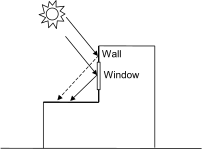
\includegraphics[width=0.9\textwidth, height=0.9\textheight, keepaspectratio=true]{media/image004.jpg}
\caption{Timestep Sequence with EMS Calling Points \protect \label{fig:timestep-sequence-with-ems-calling-points}}
\end{figure}

\begin{figure}[hbtp] % fig 3
\centering

\includegraphics[width=0.9\textwidth, height=0.9\textheight, keepaspectratio=true]{media/image005.jpg}
\caption{System Timestep Sequence with EMS Calling Points \protect \label{fig:system-timestep-sequence-with-ems-calling}}
\end{figure}

When EnergyPlus runs a model, it first does various sizing and setup activities and then models the environment periods you ask for; e.g., design days and run periods. The built-in variable called CurrentEnvironment indentifies which of these is being simulated and any given time. Figure~\ref{fig:overall-program-flow-and-ems-calling-points} diagrams the overall program flow starting at the top and listing certain key steps in outline form. EnergyPlus models contain a lot of input, and the internal processes to acquire and process that input take some time to complete. Before the model starts doing final calculations, it may have to do various sizing calculations and automatically design the size of components. It will also go through special setup periods that model a truncated set of timesteps for each environment period. In the diagram, this initial phase is not finished until just before the design periods begin. Two EMS calling points that occur only once in a given run, EndOfZoneSizing and EndOfSystemSizing, can be triggered during this initial setup phase. During the phase called ``Setup Simulation,'' the various timestep-based calling points diagrammed in Figure~\ref{fig:timestep-sequence-with-ems-calling-points} will also be called.

Another thing that happens during the setup phase described above is that individual HVAC component models access their input data and do various setup calculations in preparation for the rest of the simulation.~~ An EMS calling point (added for Version 7) called ``AfterComponentInputReadIn'' is available for selected HVAC components that allows triggering Erl programs at a point just after the component's input data have been read in but before the component's sizing routines have executed.~ This calling point is intended to be used with various actuators that are setup to override the autosize values that result from sizing.

To model environment periods, EnergyPlus runs through a serious of timesteps. Figure~\ref{fig:timestep-sequence-with-ems-calling-points} diagrams the program flow for a single timestep where the timestep for the system modeling is equal to that for the zone load modeling. The \emph{system} timestep can be shorter than the \emph{zone} timestep. The usual process of modeling a timestep is to first calculate the zone loads during the ``Predictor,'' then model the response of the HVAC systems, and then calculate the resulting zone conditions during the ``Corrector.''~ Within the HVAC system modeling, some system iterations are used to iteratively solve a system of systems. Figure~\ref{fig:system-timestep-sequence-with-ems-calling} is a slightly modified version Figure~\ref{fig:timestep-sequence-with-ems-calling-points} that diagrams the situation when the timestep of the system calculations has been reduced to half the length of the zone timestep.


\section{Begin New Environment}\label{begin-new-environment}

The calling point referred to with the keyword ``BeginNewEnvironment'' occurs once near the beginning of each environment period. Environment periods include sizing periods, design days, and run periods. This calling point will not be useful for control actions, but is useful for initializing variables and calculations that do not need to be repeated during each timestep. Once a value is set, Erl variables remember the value during the course of a simulation. Considerable repetition can be avoided by designing Erl programs to use this calling point for initializations and calculations that are needed only once. It is not called during individual timesteps.


\section{After New Environment Warmup Is Complete}\label{after-new-environment-warmup-is-complete}

The calling point referred to with the keyword ``AfterNewEnvironmentWarmUpIsComplete'' occurs once near at the beginning of each environment period but after any warmup days are complete. This is similar to the previous calling point. Warmup days are used to condition the transient aspects of the model before proceeding with the first day. This will not be useful for control actions, but would be useful for reinitializing Erl programs with fresh values after the warmup days have finished running and the model is about to start the final timestep calculations for a particular environment period.


\section{Begin Zone Timestep Before Init Heat Balance}\label{begin-timestep-before-predictor}

The calling point called ``BeginZoneTimestepBeforeInitHeatBalance'' occurs at the beginning of each timestep before ``InitHeatBalance'' executes but after the weather manager and exterior energy use manager. ``InitHeatBalance'' refers to the step in EnergyPlus modeling when the solar shading, daylighting, and surface heat balances are calculated. This calling point is useful for controlling components that affect the building envelope including surface constructions, window shades, and shading surfaces. Programs called from this point might actuate the building envelope or internal gains based on current weather or on the results from the previous timestep. Demand management routines might use this calling point to operate window shades, change active window constructions, activate exterior shades, etc.

\section{Begin Timestep Before Predictor}\label{begin-timestep-before-predictor}

The calling point called ``BeginTimestepBeforePredictor'' occurs near the beginning of each timestep but before the predictor executes. ``Predictor'' refers to the step in EnergyPlus modeling when the zone loads are calculated. This calling point is useful for controlling components that affect the thermal loads the HVAC systems will then attempt to meet. Programs called from this point might actuate internal gains based on current weather or on the results from the previous timestep. Demand management routines might use this calling point to reduce lighting or process loads, change thermostat settings, etc.


\section{After Predictor Before HVAC Managers}\label{after-predictor-before-hvac-managers}

The calling point called ``AfterPredictorBeforeHVACManagers'' occurs after predictor and before the traditional HVAC managers are called. It occurs at each timestep just after the predictor executes but before SetpointManager and AvailabilityManager models are called. It is useful for a variety of control actions. However, if there are conflicts, the EMS control actions could be overwritten by other SetpointManager or AvailabilityManager actions.


\section{After Predictor After HVAC Managers}\label{after-predictor-after-hvac-managers}

The calling point called ``AfterPredictorAfterHVACManagers'' occurs after the predictor and after the traditional HVAC managers have been called. It occurs at each timestep after the predictor executes and after the SetpointManager and AvailabilityManager models are called. It is useful for a variety of control actions. However, if there are conflicts, SetpointManager or AvailabilityManager actions may be overwritten by EMS control actions.


\section{Inside HVAC System Iteration Loop}\label{inside-hvac-system-iteration-loop}

The calling point called ``InsideHVACSystemIterationLoop'' occurs before HVAC systems are modeled. Within a timestep, EnergyPlus loops over the HVAC model to solve a system of systems. It recurs after each HVAC system iteration within each timestep and can be used for a variety of control actions that affect system operation. Being within the iteration loop can increase the accuracy of control modeling when the inputs to the controls are also changing interactively. The disadvantage is extra computational expense.


\section{End of Zone Timestep Before Reporting}\label{end-of-zone-timestep-before-reporting}

The calling point called ``EndOfZoneTimestepBeforeZoneReporting'' occurs near the end of a zone timestep but before output variable reporting is finalized. It is useful for custom output variables that use the ZoneTimestep reporting frequency.


\section{End of Zone Timestep After Reporting}\label{end-of-zone-timestep-after-reporting}

The calling point called ``EndOfZoneTimestepAfterZoneReporting'' occurs at the end of a zone timestep after output variable reporting is finalized. It is useful for preparing calculations that will go into effect the next timestep. Its capabilities are similar to BeginTimestepBeforePredictor, except that input data for current time, date, and weather data align with different timesteps.


\section{End of System Timestep Before HVAC Reporting}\label{end-of-system-timestep-before-hvac-reporting}

The calling point called ``EndOfSystemTimestepBeforeHVACReporting'' occurs near the end of a system timestep but before output variable reporting is finalized. It is useful for custom output variables that use the SystemTimestep reporting frequency.


\section{End of System Timestep After HVAC Reporting}\label{end-of-system-timestep-after-hvac-reporting}

The calling point called ``EndOfSystemTimestepAfterHVACReporting'' occurs at the end of a system timestep after output variable reporting is finalized.


\section{End of Zone Sizing}\label{end-of-zone-sizing}

The calling point called ``EndOfZoneSizing'' is used to alter the results of zone sizing calculations. It executes only once per simulation during the early stages and only if the model includes zone sizing calculations. It is not useful for control applications.


\section{End of System Sizing}\label{end-of-system-sizing}

The calling point called ``EndOfSystemSizing'' is used to alter the results of air system sizing calculations. It executes only once per simulation and is not useful for control applications.


\section{After Component Model Input has Been Read In}\label{after-component-model-input-has-been-read-in}

The calling point called ``AfterComponentInputReadIn'' is used to alter the results of individual autosize fields.~ It executes whenever one of the selected components has finished reading in its input data.~ Those, and only those, component models that have some type of actuator with an ``Autosized'' control type will also have this calling point.~ This same calling point identifier is used for different HVAC components so programs executed from this point will be repeated.~ Currently this calling point exists in three different places:~ (1) after DX coil input, (2) after fan input, and (3) after unitary system input.


\section{User Defined Component Model}\label{user-defined-component-model}

The calling point called ``UserDefinedComponentModel'' is used with Erl programs that are associated with user defined component models.~ This calling point is executed whenever a user-defined component model is called to simulate.~ The user defined component models track which program calling managers are associated with the specific component and only those calling managers are executed when this calling point is triggered. This calling point is only used with calling managers referenced by the following input objects: PlantComponent:UserDefined, Coil:UserDefined, ZoneHVAC:ForcedAir:UserDefined, or AirTerminal:SingleDuct:UserDefined.


\chapter{User-Defined Component Models}\label{user-defined-component-models}

This section provides an overview of how you can use EMS to create your own custom models for HVAC and plant equipment.~ EMS can be used not only for controls and overriding the behavior of existing models, but also to implement entirely new component models of your own formulation.~ Such user-defined component models are implemented by writing Erl programs, setting up internal variables, sensors, actuators and output variables that work in conjunction with a set of special input objects in the group called ``User Defined HVAC and Plant Component Models.''

This system provides a means of modeling new types of equipment that do not yet have models implemented in EnergyPlus.~ The capability to add new custom models should have a wide variety of creative applications such as evaluating the annual energy performance implications of new types of equipment and providing a mechanism for including ``exceptional calculation methods'' in your EnergyPlus models.

This section first introduces common characteristics of the user-defined component models and then goes into more detail on each of available component modeling shells that are used to connect user-defined models and algorithms to the rest of EnergyPlus' HVAC and plant simulations.


\section{Common Characteristics}\label{common-characteristics}

In general, each of the user-defined components will:

\begin{itemize}
\item
  Setup new EMS internal variables for the state conditions entering the component at each inlet node being used.~ Internal variables serve a similar role as Sensors in terms of obtaining input data.~ The difference is that they are updated just before the component model programs execute and therefore do not suffer the timestep lag issues that can be associated with sensors tied to output variables.~ Whereas most EMS internal variables are constants, those intended for use with user-defined components are filled each time the component is simulated and vary over time with the most current data available.
\item
  Setup new EMS actuators for the state conditions at each outlet node being used.~ These actuators are not optional and must be used.~ For each air or plant connection with an active outlet node, the associated actuators must be used and filled with valid values in order for the component model to be properly coupled to the rest of EnergyPlus.~ Some of the components will also set the results at their inlet node, for example to request a mass flow rate.
\item
  Trigger one or more specific program calling manager(s) to execute EMS programs that are called to initialize, register, and size the component model.
\item
  Trigger one or more specific program calling manager(s) to execute EMS programs that are called to actually model the component when it is called to be simulated.
\end{itemize}

The various user-defined components have some similar input fields.~ Once the user gains familiarity with one of the components, many of the concepts will carry over to the other user-defined components.~ The separate objects are primarily for the purpose of distinguishing how user-defined components need to vary in order to fit with the rest of EnergyPlus.


\section{Zone Forced Air Unit}\label{zone-forced-air-unit}

The input object called ZoneHVAC:ForcedAir:UserDefined provides a shell for creating custom models of a device that serves as a single-zone HVAC unit that operates by circulating air in and out of the zone.~ This device is analogous to those component models in the Group -- Zone Forced Air Units, such as ZoneHVAC:PackagedTerminalAirConditioner or ZoneHVAC:WaterToAirHeatPump.

In addition to the primary air connection that connects to the zone, there are options for additional connections to a second air stream (e.g.~for outdoor ventilation or heat source or sink), up to three separate plant loop connections (e.g.~hot water, chilled water, heat rejection), a water supply tank, a water collection tank, and a separate zone for skin losses.

The zone unit is associated with a thermal zone (by the ZoneHVAC:EquipmentConnections and ZoneHVAC:EquipmentList objects).~ In EnergyPlus, when there are controlled thermal zones with thermostat (and humidistat) controls, the central routines predict the loads that zone equipment need to meet in order to maintain control of the zone conditions.~ When there are multiple types of equipment serving a zone, they are sequenced to meet heating or cooling loads in a particular order.~ Rather than the total predicted load, the second or third devices need to know the load that remains after the earlier-sequenced devices have already operated on the zone.~ The following internal variables are useful inputs for controlling zone equipment in your models:

\begin{itemize}
\item
  An internal variable called ``Remaining Sensible Load to Heating Setpoint'' provides the current value for the sensible load, in {[}W{]}, that remains for this device that if delivered will allow the zone to reach the heating setpoint under current conditions.
\item
  An internal variable called ``Remaining Sensible Load to Cooling Setpoint'' provides the current value for the sensible load, in {[}W{]}, that remains for this device that if delivered will allow the zone to reach the cooling setpoint under current conditions.
\item
  An internal variable called ``Remaining Latent Load to Humidifying Setpoint'' provides the current value for the latent load, in {[}kg/s{]}, that remains for this device that if delivered will allow the zone to reach the humidification setpoint under current conditions.
\item
  An internal variable called ``Remaining Latent Load to Dehumidifying Setpoint'' provides the current value for the latent load, in {[}kg/s{]}, that remains for this device that if delivered will allow the zone to reach the dehumidification setpoint under current conditions.
\end{itemize}

\subsection{Primary Air Connection}\label{primary-air-connection-000}

The primary air connection includes both an inlet and an outlet that are required to be used when using this component.~ This is called the primary air connection because it is how the zone unit is connected to the zone.~ The inlet to the custom zone unit is a node that is also an exhaust outlet from the zone.~ The following EMS internal variables are made available for this inlet node and should be useful inputs to your own custom models:

\begin{itemize}
\item
  An internal variable called ``Inlet Temperature for Primary Air Connection,'' provides the current value for the drybulb air temperature at the component's inlet node, in {[}C{]}.
\item
  An internal variable called ``Inlet Humidity Ratio for Primary Air Connection,'' provides the current value for the moist air humidity ratio at the component's inlet node, in {[}kgWater/kgDryAir{]}
\item
  An internal variable called ``Inlet Density for Primary Air Connection,'' provides the current value for the density of moist air at the component's main inlet node, in {[}kg/m\(^{3}\){]}.
\item
  An internal variable called ``Inlet Specific Heat for Primary Air Connection,'' provides the current value for the specific heat of moist air at the component's main inlet node, in {[}J/kg-C{]}.
\end{itemize}

The inlet node also has an actuator associated with it so that the rate of air flow leaving the thermal zone and entering the unit can be passed to the rest of EnergyPlus.

\begin{itemize}
\tightlist
\item
  An actuator called ``Primary Air Connection,'' with the control type ``Inlet Mass Flow Rate,'' in {[}kg/s{]}, needs to be used.~ This will set the flow rate of air leaving the zone through the zone exhaust air node.
\end{itemize}

The primary outlet for the custom zone unit is a node that is also an inlet to the zone.~ The following EMS actuators are created for this outlet node and must be used to pass results from the custom model to the rest of EnergyPlus:

\begin{itemize}
\item
  An actuator called ``Primary Air Connection,'' with the control type ``Outlet Temperature,'' in {[}C{]}, needs to be used.~ This will set the drybulb temperature of the air leaving the zone unit and entering the zone through the zone air inlet node.
\item
  An actuator called ``Primary Air Connection,'' with the control type ``Outlet Humidity Ratio,'' in {[}kgWater/kgDryAir{]}, needs to be used.~ This will set the humidity ratio of the air leaving the zone unit and entering the zone through the zone air inlet node.
\item
  An actuator called ``Primary Air Connection,'' with the control type ``Outlet Mass Flow Rate,'' in {[}kg/s{]}, needs to be used.~ This will set the flow rate of air leaving the zone unit and entering the zone through the zone air inlet node.
\end{itemize}

It is not required that the primary air connections inlet and outlet mass flow rates be identical.~ However, if there is an imbalance, then the model should use the secondary air connection to balance air mass flows.

\subsection{Secondary Air Connection}\label{secondary-air-connection-000}

The secondary air connection provides options for an added inlet node, or outlet node, or both depending on the user's needs.~ This separate air stream can be used for outdoor air ventilation or as a source or sink for energy.~ The secondary air inlet node will often be defined to be an outdoor air node (ref. OutdoorAir:Node) but that is not required.~ The secondary air outlet node can be used as relief exhaust when the unit is providing outdoor air ventilation.~ If the secondary air outlet is not really connected to anything else and just releases air to the outdoors, then it isn't necessary that moist air properties be set using actuators because they will not impact anything else in the model.

If the secondary air connection inlet node is used, then the following internal variables and actuator are made available:

\begin{itemize}
\item
  An internal variable called ``Inlet Temperature for Secondary Air Connection,'' provides the current value for the drybulb air temperature at the secondary inlet node, in {[}C{]}.
\item
  An internal variable called ``Inlet Humidity Ratio for Secondary Air Connection,'' provides the current value for the moist air humidity ratio at the secondary inlet node, in {[}kgWater/kgDryAir{]}
\item
  An internal variable called ``Inlet Density for Secondary Air Connection,'' provides the current value for the density of moist air at the secondary inlet node, in {[}kg/m\(^{3}\){]}.
\item
  An internal variable called ``Inlet Specific Heat for Secondary Air Connection,'' provides the current value for the specific heat of moist air at the secondary inlet node, in {[}J/kg-C{]}.
\item
  An actuator called ``Secondary Air Connection,'' with the control type ``Inlet Mass Flow Rate,'' in {[}kg/s{]}, needs to be used.~ This will set the flow rate of air entering the zone unit through the secondary air connection inlet.
\end{itemize}

If the secondary air connection outlet node is used, then the following actuators are created:

\begin{itemize}
\item
  An actuator called ``Secondary Air Connection,'' with the control type ``Outlet Temperature,'' in {[}C{]}, needs to be used.~ This will set the drybulb temperature of the air leaving the zone unit through the secondary air outlet node.
\item
  An actuator called ``Secondary Air Connection,'' with the control type ``Outlet Humidity Ratio,'' in {[}kgWater/kgDryAir{]}, needs to be used.~ This will set the humidity ratio of the air leaving the zone unit through the secondary air outlet node.
\item
  An actuator called ``Secondary Air Connection,'' with the control type ``Outlet Mass Flow Rate,'' in {[}kg/s{]}, needs to be used.~ This will set the flow rate of air leaving the zone unit through the secondary air outlet node.
\end{itemize}

\subsection{Plant Connections}\label{plant-connections-002}

The user defined zone unit can also be connected to up to three different plants to provide hydronic-based cooling, heating, and/or heat source or rejection.

Although the zone unit actively conditions the zone, from the point of view of plant they are demand components.~ These plant connections are always ``demand'' in the sense that the zone unit will place loads onto the plant loops serving it and are not configured to be able to meet plant loads in the way that supply equipment could (loading mode is always DemandsLoad).~ These plant connections are always of the type that when flow is requested, the loop will be operated to try and meet the flow request and if not already running, these flow requests can turn on the loop (loop flow request mode is always NeedsFlowAndTurnsLoopOn).

For plant loops, both the inlet and outlet nodes need to be used for each loop connection.~ The ZoneHVAC:ForcedAir:UserDefined object appears directly on the Branch object used to describe the plant.~ The central plant routines require that each plant component be properly initialized and registered. Special actuators are provided for these initializations and they should be filled with values by the Erl programs that are called by the program calling manager assigned to the zone unit for model setup and sizing.~ The following three actuators are created for each of ``\emph{N}'' plant loops and must be used to properly register the plant connection:

\begin{itemize}
\item
  An actuator called ``Plant Connection \emph{N}'' with the control type ``Minimum Mass Flow Rate,'' in {[}kg/s{]}, should be used.~ This will set the so-called hardware limit for component's minimum mass flow rate when operating.~ (If not used, then the limit will be set to zero which may be okay for many if not most models.)
\item
  An actuator called ``Plant Connection \emph{N}'' with the control type ``Maximum Mass Flow Rate,'' in {[}kg/s{]}, needs to be used.~ This will set the so-called hardware limit for the component's maximum mass flow rate when operating.
\item
  An actuator called ``Plant Connection \emph{N}'' with the control type ``Design Volume Flow Rate,'' in {[}m\(^{3}\)/s{]}, needs to be used.~ This will register the size of the component for use in sizing the plant loop and supply equipment that will need to meet the loads.
\end{itemize}

For each plant loop connection that is used, the following internal variables are available for inputs to the custom component model:

\begin{itemize}
\item
  An internal variable called ``Inlet Temperature for Plant Connection \emph{N}'' provides the current value for the temperature of the fluid entering the component, in {[}C{]}.
\item
  An internal variable called ``Inlet Mass Flow Rate for Plant Connection \emph{N}'' provides the current value for the mass flow rate of the fluid entering the component, in {[}kg/s{]}.
\item
  An internal variable called ``Inlet Density for Plant Connection \emph{N}'' provides the current value for the density of the fluid entering the component, in {[}kg/m\(^{3}\){]}.~ This density is sensitive to the fluid type (e.g.~if using glycol in the plant loop) and fluid temperature at the inlet.
\item
  An internal variable called ``Inlet Specific Heat for Plant Connection \emph{N}'' provides the current value for the specific heat of the fluid entering the component, in {[}J/kg-C{]}. This specific heat is sensitive to the fluid type (e.g.~if using glycol in the plant loop) and fluid temperature at the inlet.
\end{itemize}

For each plant loop connection that is used, the following EMS actuators are created and must be used to pass results from the custom model to the rest of EnergyPlus:

\begin{itemize}
\item
  An actuator called ``Plant Connection \emph{N}'' with the control type ``Outlet Temperature,'' in {[}C{]}, needs to be used.~ This is the temperature of the fluid leaving the zone unit through that particular plant connection.
\item
  An actuator called ``Plant Connection N'' with the control type ``Mass Flow Rate,'' in kg/s, needs to be used. This actuator registers the component model's request for plant fluid flow.~ The actual mass flow rate through the component may be different than requested if the overall loop situation is such that not enough flow is available to meet all the various requests.~ In general, this actuator is used to lodge a request for flow, but the more accurate flow rate will be the internal variable called ``Inlet Mass Flow Rate for Plant Connection \emph{N.}''
\end{itemize}

\subsection{Water Use}\label{water-use-002}

The user defined zone unit can be connected to the water use models in EnergyPlus that allow modeling on-site storage.~ If a supply inlet water storage tank is used, then an actuator called ``Water System'' with the control type ``Supplied Volume Flow Rate,'' in m\(^{3}\)/s, needs to be used.~ This sets up the zone unit as a demand component for that storage tank.~ If a collection outlet water storage tank is used, then an actuator called ``Water System'' with the control type ``Collected Volume Flow Rate,'' in m\(^{3}\)/s, needs to be used.

\subsection{Ambient Zone}\label{ambient-zone-002}

The user defined zone unit can be connected to an ambient zone and provide internal gains to that zone.~ The zone can be different than the one that unit is connected to via the primary air connection if desired.~ This is for ``skin losses'' that the unit might have that result from inefficiencies and other non-ideal behavior.~ When an ambient zone is specified, the following actuators are created that can be used for different types of internal gains to the named zone:

\begin{itemize}
\item
  An actuator called ``Component Zone Internal Gain'' with the control type ``Sensible Heat Gain Rate,'' in {[}W{]}, is available.~ This can be used for purely convective sensible heat gains (or losses) to a zone.
\item
  An actuator called ``Component Zone Internal Gain'' with the control type ``Return Air Heat Gain Rate,'' in {[}W{]}, is available.~ This can be used for purely convective sensible heat gains (or losses) to the return air duct for a zone.
\item
  An actuator called ``Component Zone Internal Gain'' with the control type ``Thermal Radiation Heat Gain Rate,'' in {[}W{]}, is available.~ This can be used for thermal radiation gains (or losses) to a zone.
\item
  An actuator called ``Component Zone Internal Gain'' with the control type ``Latent Heat Gain Rate,' in {[}W{]}, is available.~ This can be used for latent moisture gains (or losses) to a zone.
\item
  An actuator called ``Component Zone Internal Gain'' with the control type ``Return Air Latent Heat Gain Rate,'' in {[}W{]}, is available.~ This can be used for latent moisture gains (or losses) to a the return air duct for a zone.
\item
  An actuator called ``Component Zone Internal Gain'' with the control type ``Carbon Dioxide Gain Rate,'' in {[}m\(^{3}\)/s{]}, is available.~ This can be used for carbon dioxide gains (or losses) to a zone.
\item
  An actuator called ``Component Zone Internal Gain'' with the control type ``Gaseous Contaminant Gain Rate,'' in {[}m\(^{3}\)/s{]}, is available.~ This can be used for generic gaseous air pollutant gains (or losses) to a zone.
\end{itemize}


\input{src/user-defined-component-models/air-terminal-unit}

\section{Air Coil}\label{air-coil}

The input object called Coil:UserDefined provides a shell for creating custom models for a coil that processes air as part of an air handler.~ This device is analogous to coils models such as Coil:Cooling:Water, Coil:Heating:Water, and Coil:Cooling:DX:SingleSpeed, but can also be used for heat-exchanger-like devices such as HeatExchanger:AirToAir:SensibleAndLatent or EvaporativeCooler:Indirect:WetCoil.

The user defined coil model can use one or two air connections, one optional plant connection, a water supply tank, a water collection tank, and a separate zone for skin losses.

\subsection{Air Connections}\label{air-connections}

Each of the two air connections that are available include both an inlet and an outlet node that are required for each air connection that is used.~ The Coil:UserDefined object appears directly on a Branch object used to define the supply side of an air handler, or in the AirLoopHVAC:OutdoorAirSystem:EquipmentList object used to define outdoor air systems.~ The following EMS internal variables are made available for each inlet node and should be useful inputs to your own custom models:

\begin{itemize}
\item
  An internal variable called ``Inlet Temperature for Air Connection \emph{N},'' provides the current value for the drybulb air temperature at the component's inlet node, in {[}C{]}.
\item
  An internal variable called ``Inlet Humidity Ratio for Air Connection \emph{N},'' provides the current value for the moist air humidity ratio at the component's inlet node, in {[}kgWater/kgDryAir{]}
\item
  An internal variable called ``Inlet Density for Air Connection \emph{N},'' provides the current value for the density of moist air at the component's main inlet node, in {[}kg/m\(^{3}\){]}.
\item
  An internal variable called ``Inlet Specific Heat for Air Connection \emph{N},'' provides the current value for the specific heat of moist air at the component's main inlet node, in {[}J/kg-C{]}.
\end{itemize}

The following EMS actuators are created for each outlet node and must be used to pass results from the custom model to the rest of EnergyPlus:

\begin{itemize}
\item
  An actuator called ``Air Connection \emph{N},'' with the control type ``Outlet Temperature,'' in {[}C{]}, needs to be used.~ This will set the drybulb temperature of the air leaving the coil.
\item
  An actuator called ``Air Connection \emph{N},'' with the control type ``Outlet Humidity Ratio,'' in {[}kgWater/kgDryAir{]}, needs to be used.~ This will set the humidity ratio of the air leaving the coil.
\item
  An actuator called ``Air Connection \emph{N},'' with the control type ``Mass Flow Rate,'' in {[}kg/s{]}, needs to be used.~ This will set the flow rate of air leaving the coil.
\end{itemize}

\subsection{Plant Connections}\label{plant-connections}

The user defined coil can also be connected to one plant loop to provide hydronic-based cooling, heating, or heat source or rejection.

Although the coil actively conditions the air stream passing through it, from the point of view of plant it is a demand component.~ This plant connection is always ``demand'' in the sense that the coil will place loads onto the plant loop serving it and is not configured to be able to meet plant loads in the way that supply equipment could (loading mode is always DemandsLoad).~ This plant connection is always of the type that when flow is requested, the loop will be operated to try and meet the flow request and if not already running, these flow requests can turn on the loop (loop flow request mode is always NeedsFlowAndTurnsLoopOn).

Both the inlet and outlet nodes need to be used is a loop is connected.~ The Coil:UserDefined object appears directly on the Branch object used to describe the plant.~ The central plant routines require that each plant component be properly initialized and registered. Special actuators are provided for these initializations and they should be filled with values by the Erl programs that are called by the program calling manager assigned to the coil for model setup and sizing.~ The following three actuators are created for the plant loop and must be used to properly register the plant connection:

\begin{itemize}
\item
  An actuator called ``Plant Connection'' with the control type ``Minimum Mass Flow Rate,'' in {[}kg/s{]}, should be used.~ This will set the so-called hardware limit for component's minimum mass flow rate when operating.~ (If not used, then the limit will be set to zero which may be okay for many if not most models.)
\item
  An actuator called ``Plant Connection'' with the control type ``Maximum Mass Flow Rate,'' in {[}kg/s{]}, needs to be used.~ This will set the so-called hardware limit for the component's maximum mass flow rate when operating.
\item
  An actuator called ``Plant Connection'' with the control type ``Design Volume Flow Rate,'' in {[}m\(^{3}\)/s{]}, needs to be used.~ This will register the size of the component for use in sizing the plant loop and supply equipment that will need to meet the loads.
\end{itemize}

When the plant loop connection is used, the following internal variables are available for inputs to the custom component model:

\begin{itemize}
\item
  An internal variable called ``Inlet Temperature for Plant Connection'' provides the current value for the temperature of the fluid entering the component, in {[}C{]}.
\item
  An internal variable called ``Inlet Mass Flow Rate for Plant Connection'' provides the current value for the mass flow rate of the fluid entering the component, in {[}kg/s{]}.
\item
  An internal variable called ``Inlet Density for Plant Connection'' provides the current value for the density of the fluid entering the component, in {[}kg/m\(^{3}\){]}.~ This density is sensitive to the fluid type (e.g.~if using glycol in the plant loop) and fluid temperature at the inlet.
\item
  An internal variable called ``Inlet Specific Heat for Plant Connection'' provides the current value for the specific heat of the fluid entering the component, in {[}J/kg-C{]}. This specific heat is sensitive to the fluid type (e.g.~if using glycol in the plant loop) and fluid temperature at the inlet.
\end{itemize}

When the plant loop connection is used, the following EMS actuators are created and must be used to pass results from the custom model to the rest of EnergyPlus:

\begin{itemize}
\item
  An actuator called ``Plant Connection'' with the control type ``Outlet Temperature,'' in {[}C{]}, needs to be used.~ This is the temperature of the fluid leaving the coil.
\item
  An actuator called ``Plant Connection'' with the control type ``Mass Flow Rate,'' in kg/s, needs to be used. This actuator registers the component model's request for plant fluid flow.~ The actual mass flow rate through the component may be different than requested if the overall loop situation is such that not enough flow is available to meet all the various requests.~ In general, this actuator is used to lodge a request for flow, but the more accurate flow rate will be the internal variable called ``Inlet Mass Flow Rate for Plant Connection\emph{.}''
\end{itemize}

\subsection{Water Use}\label{water-use}

The user defined coil can be connected to the water use models in EnergyPlus that allow modeling on-site storage.~ If a supply inlet water storage tank is used, then an actuator called ``Water System'' with the control type ``Supplied Volume Flow Rate,'' in m\(^{3}\)/s, needs to be used.~ This sets up the coil as a demand component for that storage tank.~ If a collection outlet water storage tank is used, then an actuator called ``Water System'' with the control type ``Collected Volume Flow Rate,'' in m\(^{3}\)/s, needs to be used.

\subsection{Ambient Zone}\label{ambient-zone}

The user defined coil can be connected to an ambient zone and provide internal gains to that zone.~ This is for ``skin losses'' that the coil might have that result from inefficiencies and other non-ideal behavior.~ When an ambient zone is specified, the following actuators are created that can be used for different types of internal gains to the named zone:

\begin{itemize}
\item
  An actuator called ``Component Zone Internal Gain'' with the control type ``Sensible Heat Gain Rate,'' in {[}W{]}, is available.~ This can be used for purely convective sensible heat gains (or losses) to a zone.
\item
  An actuator called ``Component Zone Internal Gain'' with the control type ``Return Air Heat Gain Rate,'' in {[}W{]}, is available.~ This can be used for purely convective sensible heat gains (or losses) to the return air duct for a zone.
\item
  An actuator called ``Component Zone Internal Gain'' with the control type ``Thermal Radiation Heat Gain Rate,'' in {[}W{]}, is available.~ This can be used for thermal radiation gains (or losses) to a zone.
\item
  An actuator called ``Component Zone Internal Gain'' with the control type ``Latent Heat Gain Rate,' in {[}W{]}, is available.~ This can be used for latent moisture gains (or losses) to a zone.
\item
  An actuator called ``Component Zone Internal Gain'' with the control type ``Return Air Latent Heat Gain Rate,'' in {[}W{]}, is available.~ This can be used for latent moisture gains (or losses) to a the return air duct for a zone.
\item
  An actuator called ``Component Zone Internal Gain'' with the control type ``Carbon Dioxide Gain Rate,'' in {[}m\(^{3}\)/s{]}, is available.~ This can be used for carbon dioxide gains (or losses) to a zone.
\item
  An actuator called ``Component Zone Internal Gain'' with the control type ``Gaseous Contaminant Gain Rate,'' in {[}m\(^{3}\)/s{]}, is available.~ This can be used for generic gaseous air pollutant gains (or losses) to a zone.
\end{itemize}


\section{Plant Component}\label{plant-component}

The input object called PlantComponent:UserDefined provides a shell for creating custom models of a device that is part of the plant models used for hydronic-type systems.~ This object can be used for primary heating or cooling devices, such as boilers or chillers.

Although the other user-defined component models can also connect to plant, they are always simple ``demand'' components (from the point of view of plant modeling) and their calls to simulate are led by the air side portions of the program's calling tree.~ The plant-centric component here however, is called to simulate along with other plant components (in flow order) by plant's central routines.

The user defined plant component can use up to four different plant loop connections, one optional air connection, a water supply tank, a water collection tank, and an ambient zone for skin losses.

\subsection{Plant Connections (User Defined)}\label{plant-connections-001}

The user defined plant component can be connected to up to four different plant loops.

For plant loops, both the inlet and outlet nodes need to be used for each loop connection.~ The PlantComponent:UserDefined object appears directly on the Branch object used to describe the plant.~ The central plant routines require that each plant component be properly initialized and registered. Special actuators are provided for these initializations and they should be filled with values by the Erl programs that are called by the program calling manager assigned to that particular loop connection for model setup and sizing.~ The following six actuators are created for each of ``\emph{N}'' plant loops and must be used to properly register the plant connection:

\begin{itemize}
\item
  An actuator called ``Plant Connection \emph{N}'' with the control type ``Minimum Mass Flow Rate,'' in {[}kg/s{]}, should be used.~ This will set the so-called hardware limit for component's minimum mass flow rate when operating.~ (If not used, then the limit will be set to zero which may be okay for many if not most models.)
\item
  An actuator called ``Plant Connection \emph{N}'' with the control type ``Maximum Mass Flow Rate,'' in {[}kg/s{]}, needs to be used.~ This will set the so-called hardware limit for the component's maximum mass flow rate when operating.
\item
  An actuator called ``Plant Connection \emph{N}'' with the control type ``Design Volume Flow Rate,'' in {[}m\(^{3}\)/s{]}, needs to be used.~ This will register the size of the component for use in sizing the plant loop and supply equipment that will need to meet the loads.
\item
  An actuator called ``Plant Connection \emph{N}'' with the control type ``Minimum Loading Capacity,'' in {[}W{]}, needs to be used if the device is to be used as a supply component with load-based operation schemes.
\item
  An actuator called ``Plant connection \emph{N}'' with the control type ``Maximum Loading Capacity,'' in {[}W{]}, needs to be used if the device is to be used as a supply component with load-based operation schemes.
\item
  An actuator called ``Plant Connection \emph{N}'' with the control type ``Optimal Loading Capacity,'' in {[}W{]}, needs to be used if the device is to be used as a supply component with load-based operation schemes.
\end{itemize}

For each plant loop connection that is used, the following internal variables are available for inputs to the custom component model:

\begin{itemize}
\item
  An internal variable called ``Inlet Temperature for Plant Connection \emph{N}'' provides the current value for the temperature of the fluid entering the component, in {[}C{]}.
\item
  An internal variable called ``Inlet Mass Flow Rate for Plant Connection \emph{N}'' provides the current value for the mass flow rate of the fluid entering the component, in {[}kg/s{]}.
\item
  An internal variable called ``Inlet Density for Plant Connection \emph{N}'' provides the current value for the density of the fluid entering the component, in {[}kg/m\(^{3}\){]}.~ This density is sensitive to the fluid type (e.g.~if using glycol in the plant loop) and fluid temperature at the inlet.
\item
  An internal variable called ``Inlet Specific Heat for Plant Connection \emph{N}'' provides the current value for the specific heat of the fluid entering the component, in {[}J/kg-C{]}. This specific heat is sensitive to the fluid type (e.g.~if using glycol in the plant loop) and fluid temperature at the inlet.
\item
  An internal variable called ``Load Request for Plant Connection N'' provides the current value for the desired operating capacity, in {[}W{]}.~ This is the input for how the model is being asked to meet the loads on the supply side.~ This is the result of the central routines for operation schemes and should be useful for controlling a plant model.~ (This internal variable is not made available when this plant connection's loading mode is set to DemandsLoad.)
\end{itemize}

For each plant loop connection that is used, the following EMS actuators are created and must be used to pass results from the custom model to the rest of EnergyPlus:

\begin{itemize}
\item
  An actuator called ``Plant Connection \emph{N}'' with the control type ``Outlet Temperature,'' in {[}C{]}, needs to be used.~ This is the temperature of the fluid leaving the air terminal unit through that particular plant connection.
\item
  An actuator called ``Plant Connection \emph{N}'' with the control type ``Mass Flow Rate,'' in kg/s, needs to be used. This actuator registers the component model's request for plant fluid flow.~ The actual mass flow rate through the component may be different than requested if the overall loop situation is such that not enough flow is available to meet all the various requests.~ In general, this actuator is used to lodge a request for flow, but the more accurate flow rate will be the internal variable called ``Inlet Mass Flow Rate for Plant Connection \emph{N.}''
\end{itemize}

For each plant loop connection that is used, there is input required to specify the nature of the connection with respect to loads.~ One of the following choices must be selected depending on the purpose of the component model.

\begin{itemize}
\item
  DemandsLoad. This type of loading is used for plant connections that place a load on the loop.~ Connections that use this loading scheme are not set up to meet loads and interact with the operation schemes.~ For example, this loading mode is appropriate for the condenser side of a chiller.
\item
  MeetsLoadWithPassiveCapacity.~ This type of loading is used for plant connections where the component has some capacity to meet loads but it is not really of the type that could be controlled.~ For example, a ground heat exchanger is passive because while it can provide some level of heat rejection or source, the amount will vary with current conditions and cannot usually be explicitly controlled.
\item
  MeetsLoadWithNominalCapacity.~ This type of loading is used for plant connections where the component has controllable capacity to meet loads and no outlet temperature restrictions.
\item
  MeetsLoadWithNominalCapacityLowOutLimit.~ This type of loading is used for plant connections where the component has controllable capacity to meet loads but with a lower limit on the fluid temperature at the outlet node.~ For example, this can be used for a chiller evaporator connection when the chiller is prevented from producing chilled water below a certain temperature limit.~ When this type of loading is selected, an actuator is created to allow setting the low temperature limit for use by the load dispatch routines.~ The actuator is called ``Plant Connection \emph{N}'' with the control type ``Low Outlet Temperature Limit,'' in {[}C{]}, and needs to be used.
\item
  MeetsLoadWithNominalCapacityHiOutLimit.~ This type of loading is used for plant connections where the component has controllable capacity to meet loads but with an upper limit on the fluid temperature at the outlet node.~ For example, this can be used for a boiler connection when the boiler is prevented from producing hot water above a certain temperature limit.~ When this type of loading is selected, an actuator is created to allow setting the high temperature limit for use by the load dispatch routines.~ The actuator is called ``Plant Connection \emph{N}'' with the control type ``High Outlet Temperature Limit,'' in {[}C{]}, and needs to be used.
\end{itemize}

For each plant loop connection, there is input required for the nature of the flow requests made by the component with respect to determining the overall flow for the loop.~ Mass flow request are also important for resolving the flow rates in parallel branches, but the mode here is related to the problem of determining the overall flow rate for the loop, not the flow down one particular branch.~ The overall loop flow rate is a function of all the flow requests made by the different devices on the loop and different types of devices have different implications for the overall loop rate.~ One of the following three choices must be made depending on the nature of the plant component.

\begin{itemize}
\item
  NeedsFlowIfLoopOn.~ Devices with this flow request mode will contribute to the overall loop flow rate but will not initiate flow themselves.~ Other devices on the plant loop (of type NeedsFlowAndTurnsLoopOn ) need to make flow requests to get the loop flowing at all, but once it is flowing, this device can affect the overall loop flow rate.~ For example, a chiller may have a lower limit on the allowable chilled water flow rate through its evaporator and if that lower limit is higher than the current request for chilled water by the cooling coils, then the overall loop flow will be that needed by the chiller rather than the coils.
\item
  NeedsFlowAndTurnsLoopOn.~ Devices with this flow request mode will contribute to the overall loop flow rate and initiate flow themselves.~ This mode is used for demand component such as coils.~ Devices with this mode will initiate loops to turn on and start moving fluid.
\item
  ReceivesWhateverFlowAvailable.~ Devices with this flow request mode will not contribute to the overall loop flow rate and do not initiate flow themselves.~ These are essentially passive devices that take whatever flow is sent to them, such as a ground heat exchanger.
\end{itemize}

Separate program calling managers are available for each plant loop connection.~ The user defined plant component is called to simulate by the central plant routines (whereas the other user defined components are called by the central HVAC routines).~ The calls to simulate are made for each connection and you may want or need to perform different model calculations depending on which plant loop connection is being simulated at the time.~ There is an Erl program calling manager for initialization, setup, and sizing that needs to be used \emph{for each plant connection} and is only called during the early plant loop initialization phase.~ There is also an Erl program calling manager for the model calculations to perform for each plant connection.

\subsection{Plant Component (Temperature Source)}\label{plant-component-temperature-source}

An actuator called ``PlantComponent:TemperatureSource'' with the control type ``Maximum Mass Flow Rate'' in {[}kg/s{]} is available for controlling the maximum flow rate from a temperature source plant component.

\subsection{Air Connection}\label{air-connection}

An air connection is available that includes both an inlet and an outlet node.~ This can be used for air source or heat rejections. The following EMS internal variables are made available for the inlet node, if it is used, and should be useful inputs to your own custom models:

\begin{itemize}
\item
  An internal variable called ``Inlet Temperature for Air Connection,'' provides the current value for the drybulb air temperature at the component's inlet node, in {[}C{]}.
\item
  An internal variable called ``Inlet Mass Flow Rate for Air Connection,'' provides the current value for the mass flow rate of air at the component's inlet node, in {[}kg/s{]}.
\item
  An internal variable called ``Inlet Humidity Ratio for Air Connection,'' provides the current value for the moist air humidity ratio at the component's inlet node, in {[}kgWater/kgDryAir{]}
\item
  An internal variable called ``Inlet Density for Air Connection,'' provides the current value for the density of moist air at the component's main inlet node, in {[}kg/m\(^{3}\){]}.
\item
  An internal variable called ``Inlet Specific Heat for Air Connection,'' provides the current value for the specific heat of moist air at the component's main inlet node, in {[}J/kg-C{]}.
\end{itemize}

The following EMS actuators are created for the outlet air node, if it is used, and must be used to pass results from the custom model to the rest of EnergyPlus:

\begin{itemize}
\item
  An actuator called ``Air Connection,'' with the control type ``Outlet Temperature,'' in {[}C{]}, needs to be used.~ This will set the drybulb temperature of the air leaving the component.
\item
  An actuator called ``Air Connection,'' with the control type ``Outlet Humidity Ratio,'' in {[}kgWater/kgDryAir{]}, needs to be used.~ This will set the humidity ratio of the air leaving the component.
\item
  An actuator called ``Air Connection,'' with the control type ``Outlet Mass Flow Rate,'' in {[}kg/s{]}, needs to be used.~ This will set the flow rate of air leaving the component.
\end{itemize}

\subsection{Water Use}\label{water-use-001}

The user defined plant component can be connected to the water use models in EnergyPlus that allow modeling on-site storage.~ If a supply inlet water storage tank is used, then an actuator called ``Water System'' with the control type ``Supplied Volume Flow Rate,'' in m\(^{3}\)/s, needs to be used.~ This sets up the plant component as a demand component for that storage tank.~ If a collection outlet water storage tank is used, then an actuator called ``Water System'' with the control type ``Collected Volume Flow Rate,'' in m\(^{3}\)/s, needs to be used.

\subsection{Ambient Zone}\label{ambient-zone-001}

The user defined plant component can be connected to an ambient zone and provide internal gains to that zone.~ This is for ``skin losses'' that the component might have that result from inefficiencies and other non-ideal behavior.~ When an ambient zone is specified, the following actuators are created that can be used for different types of internal gains to the named zone:

\begin{itemize}
\item
  An actuator called ``Component Zone Internal Gain'' with the control type ``Sensible Heat Gain Rate,'' in {[}W{]}, is available.~ This can be used for purely convective sensible heat gains (or losses) to a zone.
\item
  An actuator called ``Component Zone Internal Gain'' with the control type ``Return Air Heat Sensible Gain Rate,'' in {[}W{]}, is available.~ This can be used for purely convective sensible heat gains (or losses) to the return air duct for a zone.
\item
  An actuator called ``Component Zone Internal Gain'' with the control type ``Thermal Radiation Heat Gain Rate,'' in {[}W{]}, is available.~ This can be used for thermal radiation gains (or losses) to a zone.
\item
  An actuator called ``Component Zone Internal Gain'' with the control type ``Latent Heat Gain Rate,' in {[}W{]}, is available.~ This can be used for latent moisture gains (or losses) to a zone.
\item
  An actuator called ``Component Zone Internal Gain'' with the control type ``Return Air Latent Heat Gain Rate,'' in {[}W{]}, is available.~ This can be used for latent moisture gains (or losses) to a the return air duct for a zone.
\item
  An actuator called ``Component Zone Internal Gain'' with the control type ``Carbon Dioxide Gain Rate,'' in {[}m\(^{3}\)/s{]}, is available.~ This can be used for carbon dioxide gains (or losses) to a zone.
\item
  An actuator called ``Component Zone Internal Gain'' with the control type ``Gaseous Contaminant Gain Rate,'' in {[}m\(^{3}\)/s{]}, is available.~ This can be used for generic gaseous air pollutant gains (or losses) to a zone.
\end{itemize}


\chapter{EMS Examples}\label{ems-examples}

This section provides examples that demonstrate how to use the EMS. Each example provides a problem statement, discusses how to approach a solution using EMS, and provides example EMS input objects. For each example a complete input data file is provided with the EnergyPlus release (you can find this in the ExampleFiles\textbackslash{} directory).

A range of example applications is presented here. Each is presented in isolation for simplicity, but a much more comprehensive approach to EMS programs is also possible.


\section{Example 1. Whole-Building Average Zone Air Temperature}\label{example-1.-whole-building-average-zone-air-temperature}

\subsection{Problem Statement}\label{problem-statement}

Although EnergyPlus can report an enormous number of output variables, you may want a custom report variable such as one for the average temperature in the building. Only zone-by-zone indoor air temperatures are available. Because it is nearly always important to check that models are properly controlling zone air conditions, you may need to examine air temperature results from your models. Compared to scanning across the many zones in a large building, you could save time when checking a model if you have a single value for a whole-building average temperature. Of course, you could calculate such a value after a run by postprocessing, but redoing this for every run is cumbersome and time consuming. Therefore, it would be more convenient to automatically calculate such a value inside the program and output it in the usual manner. For example, if we take the Small Office Reference Building (RefBldgSmallOfficeNew2004\_Chicago.idf), is there a way to create a custom report variable that provides a weighted average for the indoor temperature of all the occupied zones in a model?

\subsection{EMS Design Discussion}\label{ems-design-discussion}

This is a fairly simple example in that the EMS controls nothing. There are no actuators.

The example file has six zones, but one is an attic that we do not care about. Therefore, the main inputs, or EMS sensors, will be the zone air temperatures for the five occupied zones. We will use EnergyManagementSystem:Sensor objects to obtain the values for the air temperatures by mapping to the output variable called ``Zone Mean Air Temperature.''

A model for average temperature can be constructed by using the zone air volumes as weights so larger zones have more influence than smaller zones on the resulting average. The model equation we will implement in EMS for our new report variable is

\begin{equation}
T_{average} = \frac{\sum\left(T_{zone}\text{Vol}_{zone}\right)}{\sum\left(\text{Vol}_{zone}\right)}
\end{equation}

The example file specifies the zone volume in its zone objects so we have the data needed for the weighting factors from elsewhere in the IDF. However, a study could vary the geometry such that the volumes differ from one simulation to another. Zone Air Volume is available as internal data, so we will use EnergyManagementSystem:InternalVariable input objects to assign these weighting factors into global Erl variables. If we did not know beforehand that Zone Air Volume was an available internal variable, we would have had to prerun the model with some EMS-related objects and the appropriate level of reporting selected in an Output:EnergyManagementSystem object, and then studied the EDD output file. Note that the EDD file is only produced if you have EMS/Erl programs in your input file.

The custom output variable will be defined by using an EnergyManagementSystem:OutputVariable input object. This requires the Erl variable to be global, so we need to declare a variable. Let's call it AverageBuildingTemp, to be global using an EnergyManagementSystem:GlobalVariable object so we have a way to connect the result calculated in the Erl program to the custom output.

There are two main considerations when selecting an EMS calling point:

\begin{itemize}
\item
  The call should be toward the end of the zone timestep so the zone air temperature calculations are finalized.
\item
  The call should be before reporting updates so our new value is available before the reporting is finalized.
\end{itemize}

We therefore choose the EMS calling point with the key of ``EndOfZoneTimestepBeforeReporting.''

\subsection{EMS Input Objects}\label{ems-input-objects}

A set of input objects to solve this problem appears below and is included in the example file called ``EMSCustomOutputVariable.idf.''

\begin{lstlisting}

EnergyManagementSystem:Sensor,
     T1, !Name
     Perimeter_ZN_1 ,! Output:Variable or Output:Meter Index Key Name
     Zone Mean Air Temperature ; ! Output:Variable or Output:Meter Name


   EnergyManagementSystem:Sensor,
     T2, !Name
     Perimeter_ZN_2 , ! Output:Variable or Output:Meter Index Key Name
     Zone Mean Air Temperature ; ! Output:Variable or Output:Meter Name


   EnergyManagementSystem:Sensor,
     T3, !Name
     Perimeter_ZN_3 , ! Output:Variable or Output:Meter Index Key Name
     Zone Mean Air Temperature ; ! Output:Variable or Output:Meter Name


   EnergyManagementSystem:Sensor,
     T4, !Name
     Perimeter_ZN_4, ! Output:Variable or Output:Meter Index Key Name
     Zone Mean Air Temperature ;! Output:Variable or Output:Meter Name


   EnergyManagementSystem:Sensor,
     T5, !Name
     Core_ZN , ! Output:Variable or Output:Meter Index Key Name
     Zone Mean Air Temperature ; ! Output:Variable or Output:Meter Name


   EnergyManagementSystem:ProgramCallingManager,
     Average Building Temperature , ! Name
     EndOfZoneTimestepBeforeZoneReporting , ! EnergyPlus Model Calling Point
     AverageZoneTemps ; ! Program Name 1


   EnergyManagementSystem:GlobalVariable,
     AverageBuildingTemp;


   EnergyManagementSystem:OutputVariable,
     Weighted Average Building Zone Air Temperature [C], ! Name
     AverageBuildingTemp, ! EMS Variable Name
     Averaged, ! Type of Data in Variable
     ZoneTimeStep ; ! Update Frequency


   EnergyManagementSystem:InternalVariable,
     Zn1vol,
     Perimeter_ZN_1,
     Zone Air Volume;


   EnergyManagementSystem:InternalVariable,
     Zn2vol,
     Perimeter_ZN_2,
     Zone Air Volume;


   EnergyManagementSystem:InternalVariable,
     Zn3vol,
     Perimeter_ZN_3,
     Zone Air Volume;


   EnergyManagementSystem:InternalVariable,
     Zn4vol,
     Perimeter_ZN_4,
     Zone Air Volume;


   EnergyManagementSystem:InternalVariable,
     Zn5vol,
     Core_ZN ,
     Zone Air Volume;


   EnergyManagementSystem:Program,
     AverageZoneTemps , ! Name
     SET SumNumerator = T1*Zn1vol + T2*Zn2vol + T3*Zn3vol + T4*Zn4vol + T5*Zn5vol,
     SET SumDenominator = Zn1vol + Zn2vol + Zn3vol + Zn4vol + Zn5vol,
     SET AverageBuildingTemp = SumNumerator / SumDenominator;


   Output:EnergyManagementSystem,
     Verbose,
     Verbose,
     Verbose;


   Output:Variable,
     *,                       !- Key Value
     Weighted Average Building Zone Air Temperature,  !- Variable Name
     timestep;                  !- Reporting Frequency
\end{lstlisting}


\section{Example 2. Traditional Setpoint and Availability Managers}\label{example-2.-traditional-setpoint-and-availability-managers}

\subsection{Problem Statement}\label{problem-statement-004}

The traditional way of modeling supervisory control of HVAC systems in EnergyPlus is to use SetpointManagers and AvailabilityManagers. To gain experience with EMS, we should ask, Is there a way to take a model such as the Large Office Reference Building (RefBldgLargeOfficeNew2004\_Chicago.idf) and replicate the traditional HVAC managers by using only the EMS?

\subsection{EMS Design Discussion}\label{ems-design-discussion-004}

A review of the example file shows that three types of traditional HVAC managers are being used:~ scheduled setpoints, mixed air setpoints, and night cycle availability. We will discuss these separately.

The input object SetpointManager:Scheduled functions by placing a setpoint value on a specified node based on the value in a schedule. Therefore, our EMS program will do the same. First we will need to access the schedule. In this example, a schedule called Seasonal-Reset-Supply-Air-Temp-Sch contains the temperature values desired for the air system's supply deck. We use an EnergyManagementSystem:Sensor object based on the output variable called ``Schedule Value'' to fill schedule values into an Erl variable called Seasonal\_Reset\_SAT\_Sched. Once we have the sensor and actuator setup, putting the setpoint on the node involves a single line of Erl code, ``SET VAV\_1\_SAT\_setpoint = Seasonal\_Reset\_SAT\_Sched.''

The input object SetpointManager:Mixed air functions by placing a setpoint value on a specified node based on the value of the setpoint at another node and the temperature rise across the fan. The temperature rise is found by taking the temperature at the fan outlet node and subtracting the temperature at the fan inlet node. The EMS needs two additional sensors to obtain these temperatures, which are set up by using a pair EnergyManagementSystem:Sensor objects. The example file has three mixed air setpoint managers that place setpoints on the outlet of the outdoor air mixer, the outlet of the cooling coil, and the outlet of the heating coil. Therefore, we need three actuators to place setpoints at these three nodes, which are set up using three EnergyManagementSystem:Actuator objects. Each mixed air setpoint calculation is a simple single-line of program code such as ``SET VAV\_1\_CoolC\_Setpoint = Seasonal\_Reset\_SAT\_Sched - (T\_VAV1FanOut - T\_VAV1FanIn).''

The input object AvailabilityManager:NightCycle functions by monitoring zone temperature and starting up the air system (if needed) to keep the building within the thermostat range. The sensors here are the zone air temperatures, which are set up by using EnergyManagementSystem:Sensor objects in the same way as for Example 1. We will need one zone temperature sensor for each zone that is served by the air system so we can emulate the ``CycleOnAny'' model being used. The other sensors we need are the desired zone temperatures used by the thermostat. We access these temperatures directly from the schedules (HTGSETP\_SCH and CLGSETP\_SCH in the example) by using EnergyManagementSystem:Sensor objects. To control the air system's operation status, we use an EnergyManagementSystem:Actuator object that is assigned to an ``AirLoopHVAC'' component type using the control variable called ``Availability Status.''~ EnergyPlus recognizes four availability states that control the behavior of the air system. Inside EnergyPlus these are integers, but EMS has only real-valued variables, so we will use the following whole numbers:

\begin{itemize}
\item
  NoAction = 0.0
\item
  ForceOff = 1.0
\item
  CycleOn = 2.0
\item
  CycleOnZoneFansOnly = 3.0.
\end{itemize}

The traditional AvailabilityManager:NightCycle object operates by turning on the system for a prescribed amount of time (1800 seconds in the example file), and then turning it off for the same amount of time. You should be able to model this starting and stopping in EMS by using Trend variables to record the history of the actions. However, this cycling is not necessarily how real buildings are operated, and for this example we do not try to precisely emulate the traditional EnergyPlus night cycle manager. Rather, we use a simpler temperature-based control to start and stop the air system for the night cycle. The algorithm first assumes an offset tolerance of 0.83°C and calculates limits for when heating should turn on and off and when cooling should turn on and off. It then finds the maximum and minimum zone temperatures for all the zones attached to the air system. These use the @Max and @Min built-in functions, which take on two operators at a time. Then a series of logic statements is used to compare temperatures and decide what the availability status of the air system should be.

\subsection{EMS Input Objects}\label{ems-input-objects-004}

EMS examples are provided for the three types of traditional HVAC managers. The full set to run with no traditional managers is provided in the example file ``EMSReplaceTraditionalManagers\_LargeOffice.idf.''

Example input objects that replicate a scheduled setpoint manager using EMS follow.

\begin{lstlisting}

EnergyManagementSystem:Sensor,
     Seasonal_Reset_SAT_Sched, !Name
     Seasonal-Reset-Supply-Air-Temp-Sch , ! Output:Variable Index Key Name
     Schedule Value;   ! Output:Variable or Output:Meter Name


  EnergyManagementSystem:Actuator,
     VAV_1_SAT_setpoint,                ! Name
     VAV_1 Supply Equipment Outlet Node,      ! Component Name
     System Node Setpoint,              ! Component Type
     Temperature Setpoint;              ! Control Variable


  EnergyManagementSystem:Program,
     VAV_1_SchedSetpoint , ! Name
     SET VAV_1_SAT_setpoint = Seasonal_Reset_SAT_Sched;


  Example input objects that replicate a mixed air setpoint manager using EMS follow.
  EnergyManagementSystem:Sensor,
     T_VAV1FanIn, !Name
     VAV_1_HeatC-VAV_1_FanNode , ! Output:Variable Key Name
     System Node Temperature; ! Output:Variable or Output:Meter Name


  EnergyManagementSystem:Sensor,
     T_VAV1FanOut, !Name
     VAV_1 Supply Equipment Outlet Node, ! Output:Variable Index Key Name
     System Node Temperature ; ! Output:Variable or Output:Meter Name


  EnergyManagementSystem:Actuator,
     VAV_1_CoolC_Setpoint,            ! Name
     VAV_1_CoolC-VAV_1_HeatCNode ,    ! Component Name
     System Node Setpoint,            ! Component Type
     Temperature Setpoint;            ! Control Variable


  EnergyManagementSystem:Actuator,
     VAV_1_HeatC_Setpoint,                            ! Name
     VAV_1_HeatC-VAV_1_FanNode ,                  ! Component Name
     System Node Setpoint,                          ! Component Type
     Temperature Setpoint;            ! Control Variable


  EnergyManagementSystem:Actuator,
     VAV_1_OA_Setpoint,                            ! Name
     VAV_1_OA-VAV_1_CoolCNode ,                  ! Component Name
     System Node Setpoint,                          ! Component Type
     Temperature Setpoint;            ! Control Variable




  EnergyManagementSystem:Program,
     VAV1MixedAirManagers , ! Name
     SET VAV_1_CoolC_Setpoint = Seasonal_Reset_SAT_Sched - ( T_VAV1FanOut - T_VAV1FanIn),
     SET VAV_1_HeatC_Setpoint = Seasonal_Reset_SAT_Sched - ( T_VAV1FanOut - T_VAV1FanIn),
     SET VAV_1_OA_Setpoint = Seasonal_Reset_SAT_Sched - ( T_VAV1FanOut - T_VAV1FanIn);


  Example input objects for a night cycle availability manager follow.
  EnergyManagementSystem:Actuator,
    VAV_1_NightCycleStatus,   ! Name
    VAV_1,                    ! Component Name
    AirLoopHVAC,              ! Component Type
    Availability Status;      ! Control Variable




  EnergyManagementSystem:Sensor,
    heating_setpoint,                  ! Name
    HTGSETP_SCH ,         ! Output:Variable or Output:Meter Index Key Name
    Schedule Value ; ! Output:Variable or Output:Meter Name


  EnergyManagementSystem:Sensor,
    cooling_setpoint,                  ! Name
    CLGSETP_SCH ,         ! Output:Variable or Output:Meter Index Key Name
    Schedule Value ; ! Output:Variable or Output:Meter Name


  EnergyManagementSystem:Sensor,
    TzoneVAV1_1,                  ! Name
    Core_bottom ,         ! Output:Variable or Output:Meter Index Key Name
    Zone Mean Air Temperature ; ! Output:Variable or Output:Meter Name


  EnergyManagementSystem:Sensor,
    TzoneVAV1_2,                  ! Name
    Perimeter_bot_ZN_3 ,         ! Output:Variable Key Name
    Zone Mean Air Temperature ; ! Output:Variable or Output:Meter Name


  EnergyManagementSystem:Sensor,
    TzoneVAV1_3,                  ! Name
    Perimeter_bot_ZN_2 ,         ! Output:Variable Key Name
    Zone Mean Air Temperature ; ! Output:Variable or Output:Meter Name


  EnergyManagementSystem:Sensor,
    TzoneVAV1_4,                  ! Name
    Perimeter_bot_ZN_1 ,         ! Output:Variable Key Name
    Zone Mean Air Temperature ; ! Output:Variable or Output:Meter Name


  EnergyManagementSystem:Sensor,
    TzoneVAV1_5,                  ! Name
    Perimeter_bot_ZN_4 ,         ! Output:Variable Key Name
    Zone Mean Air Temperature ; ! Output:Variable or Output:Meter Name


  EnergyManagementSystem:Program,
     VAV_1_NightCycleMGR , ! Name
     SET Toffset = 0.8333  ,  ! 1.5F
     SET NoAction = 0.0 ,
     SET ForceOff = 1.0 ,
     SET CycleOn = 2.0 ,
     SET CycleOnZoneFansOnly = 3.0 ,
     SET VAV1_heating_TurnOn  = heating_setpoint - Toffset ,
     SET VAV1_heating_TurnOff = heating_setpoint + Toffset ,
     SET VAV1_cooling_TurnOn  = cooling_setpoint + Toffset ,
     SET VAV1_cooling_TurnOff = cooling_setpoint - Toffset ,
     ! find max and min for "cycleOnAny" operation
     SET Tmin = @MIN TzoneVAV1_1 TzoneVAV1_2  ,
     SET Tmin = @MIN Tmin        TzoneVAV1_3  ,
     SET Tmin = @MIN Tmin        TzoneVAV1_4  ,
     SET Tmin = @MIN Tmin        TzoneVAV1_5  ,
     SET Tmax = @MAX TzoneVAV1_1 TzoneVAV1_2  ,
     SET Tmax = @MAX Tmax        TzoneVAV1_3  ,
     SET Tmax = @MAX Tmax        TzoneVAV1_4  ,
     SET Tmax = @MAX Tmax        TzoneVAV1_5  ,
     IF Tmin < VAV1_heating_TurnOn ,
       SET VAV_1_NightCycleStatus = CycleOn,
       RETURN,  ! need to exit early or cooling check could also trigger
     ELSEIF Tmin > VAV1_heating_TurnOff,
       SET VAV_1_NightCycleStatus = NoAction,
     ENDIF,
     IF Tmax > VAV1_cooling_TurnOn,
       SET VAV_1_NightCycleStatus = CycleOn,
     ELSEIF Tmax < VAV1_cooling_TurnOff,
       SET VAV_1_NightCycleStatus = NoAction   ,
     ENDIF;
\end{lstlisting}


\section{Example 3. Hygro-thermal Window Opening Control for Airflow Network}\label{example-3.-hygro-thermal-window-opening-control-for-airflow-network}

\subsection{Problem Statement}\label{problem-statement-005}

A user of EnergyPlus version 3.1 posted the following question on the Yahoo! list (circa spring 2009):

I am currently trying to model a simple ventilation system based on an

exhaust fan and outdoor air variable aperture paths that open according to

the indoor relative humidity.

As I didn't find any object to directly do this, I am trying to use an

AirflowNetwork: MultiZone: Component: DetailedOpening object and its

AirflowNetwork: multizone: Surface object to model the variable aperture. But

the Ventilation Control Mode of the surface object can only be done via

Temperature or Enthalpy controls (or other not interesting for my purpose),

and not via humidity.

So my questions are:

1- is it possible to make the surface object variable according to the

relative humidity? (maybe adapting the program?)

2- or is there an other way to make it?

Because the traditional EnergyPlus controls for window openings do not support humidity-based controls (or did not as of Version 3.1), the correct response to Question \#1 was ``No.''~ But with the EMS, we can now answer Question \#2 as ``Yes.''~ How can we take the example file called HybridVentilationControl.idf and implement humidity-based control for a detailed opening in the airflow network model?

\subsection{EMS Design Discussion}\label{ems-design-discussion-005}

The main EMS sensor will be the zone air humidity, so we use an EnergyManagementSystem:Sensor object that maps to the output variable called System Node Relative Humidity for the zone's air node. This zone has the detailed opening.

The EMS will actuate the opening in an airflow network that is defined by the input object AirflowNetwork:MultiZone:Component:DetailedOpening. The program will setup the actuator for this internally, but we need to use an EnergyManagementSystem:Actuator object to declare that we want to use the actuator and provide the variable name we want for the Erl programs.

Because we do not know the exactly what the user had in mind, for this example we assume that the desired behavior for the opening area is that the opening should vary linearly with room air relative humidity. When the humidity increases, we want the opening to be larger. When the humidity decreases, we want the opening to be smaller. For relative humidity below 25\% we close the opening. At 60\% or higher relative humidity, the opening should be completely open. We formulate a model equation for opening factor as

\begin{equation}
F_{open} = \begin{array}{ll}
    0.0 & RH < 25\% \\
    \frac{RH-25}{60-25} & 25\% \leq RH \leq 60\% \\
    1.0 & RH > 60\%  
  \end{array}
\end{equation}

\subsection{EMS Input Objects}\label{ems-input-objects-005}

EMS-related input objects to solve this problem are listed below and are included in the example file called ``EMSAirflowNetworkOpeningControlByHumidity.idf.''

\begin{lstlisting}

EnergyManagementSystem:Sensor,
    ZoneRH , ! Name
    Zone 1 Node, ! Output:Variable or Output:Meter Index Key Name
    System Node Relative Humidity; ! Output:Variable or Output:Meter Name


  EnergyManagementSystem:Actuator,
    MyOpenFactor,                            ! Name
    Zn001:Wall001:Win001,                  ! Component Name
    AirFlow Network Window/Door Opening, ! Component Type
    Venting Opening Factor;    ! Control Type


  EnergyManagementSystem:ProgramCallingManager,
    RH Controlled Open Factor ,    ! Name
    BeginTimestepBeforePredictor , ! EnergyPlus Model Calling Point
    RH_OpeningController ;         ! Program Name 1


  EnergyManagementSystem:Program,
    RH_OpeningController ,     ! Name
    IF ZoneRH < 25,
      SET MyOpenFactor = 0.0 ,
    ELSEIF ZoneRH > 60,
      SET MyOpenFactor = 1.0 ,
    ELSE,
      SET MyOpenFactor = (ZoneRH - 25) / (60 - 25),
    ENDIF;


  Output:EnergyManagementSystem,
    Verbose,
    Verbose,
    Verbose;
\end{lstlisting}


\section{Example 4. Halt Program Based on Constraint}\label{example-4.-halt-program-based-on-constraint}

\subsection{Problem Statement}\label{problem-statement-006}

Heavy users of EnergyPlus explore the enormous parameter space associated with building design options. Computational requirements often limit what can be accomplished in a given study. For optimizations and other parametric studies, there is usually a tension between having a very detailed model that is comfortably accurate, and a simpler model that executes faster.

For most studies many trial simulations are discarded because they violate some constraint. To save computation time, you might consider ``fatal--out'' simulations where early calculations show that some predetermined constraints will not be met in the final result. Many studies could save considerable computing resources by prematurely quitting models rather than always letting each simulation run to completion. All types of constraints such as poor comfort, excessive system iterations, and high energy costs could be used to kill a run. You should ask, Is there a way to use the EMS to expedite my optimal searches by stopping models prematurely if they fail some test?

\subsection{EMS Design Discussion}\label{ems-design-discussion-006}

As an example, let us assume that the criterion for early exit is that the model fails to be sufficiently comfortable. We will start with the Small Hotel Reference Building example file (RefBldgSmallHotelNew2004\_Chicago.idf). Short periods of discomfort are tolerated, but if the space is uncomfortable over time, we want to abandon the simulation and save computational expense. A simulation can be stopped from within an Erl program by calling the built-in function ``@FatalHaltEp.''~ The EMS system has only numeric data types, so we cannot generate text for the error message. Therefore, we choose a particular real-numbered value to use as an error code that provides some detail on which constraint caused early termination. In this example, we choose the value ``1002.50'' to indicate an average PMV exceeds 2.5 and the value ``9001.30'' indicates the average PMV less than 1.3. We will formulate the constraint by using the result of the Fanger comfort model for PMV for the building's core zone named ``Core\_ZN.''~ If the occupants will be too cold, we will call @FatalHaltEp with the error code 9001.30. If the occupants will be too warm during a summer design day, we will fatal out with the error code 1002.50. (These values were chosen arbitrarily to demonstrate EMS; PMV of 1.3 is not necessarily a problem.)

To monitor PMV, we will use a trend variable, which we create by using the EnergyManagementSystem:TrendVariable input object. A trend variable is a log of historical values for Erl variables. A trend log is an array that goes farther and farther back in time. For this example, we assume the constraint is to monitor the average PMV for the previous 2-hour period. The example file has 6 timesteps per hour, so each trend point is 10 minutes and a 2-hour average needs 12 timesteps. So the field Number of Timesteps to be Logged must be 12 or larger. To access the values stored in a trend variable, the built-in functions provided for accessing trends must be used. The @TrendAverage function called with an index of 12 will return the 2-hour running average. To monitor this result of running average PMV, we set up custom output variable using an EnergyManagementSystem:OutputVariable input object.

\subsection{EMS Input Objects}\label{ems-input-objects-006}

The EMS input objects for this example follow and are contained in the example file called ``EMSTestMAthAndKill.idf.''

\begin{lstlisting}

 EnergyManagementSystem:ProgramCallingManager,
     Average Building Temperature , ! Name
     EndOfZoneTimestepBeforeZoneReporting , ! EnergyPlus Model Calling Point
     updateMy_averagePMV; ! Program Name 1

   EnergyManagementSystem:Sensor,
     PMV5, !Name
     Core_ZN , ! Output:Variable or Output:Meter Index Key Name
     Zone Thermal Comfort Fanger Model PMV ; ! Output:Variable Name

   EnergyManagementSystem:TrendVariable,
     PMVtrendLog1,
     PMV5,
     300;

   EnergyManagementSystem:GlobalVariable,
     PMVrunningAvg;

   EnergyManagementSystem:OutputVariable,
     Running Two Hour Average PMV [PMVunits], ! Name
     PMVrunningAvg, ! EMS Variable Name
     Averaged, ! Type of Data in Variable
     ZoneTimeStep ; ! Update Frequency

   EnergyManagementSystem:Program,
     UpdateMy_averagePMV,
     Set PMVrunningAvg = @TrendAverage PMVtrendLog1 12, ! two hour running average.
     RUN Kill_Run_if_Uncomfortable;

   EnergyManagementSystem:Subroutine,
     Kill_Run_if_Uncomfortable,
     IF PMVrunningAvg > 2.5,
       SET tmpError = @FatalHaltEp 1002.50, ! error code "1002.50" for comfort avg over 2.5
     ENDIF,
     IF PMVrunningAvg < 0.0 - 1.3,
       SET tmpError = @FatalHaltEp 9001.30, ! error code "9001.30" for comfort avg under - 1.3
     ENDIF;
\end{lstlisting}


\section{Example 5. Computed Schedule}\label{example-5.-computed-schedule}

\subsection{Problem Statement}\label{problem-statement-007}

Many models have schedule inputs that could be used to control the object, but creating the schedules it is too cumbersome. We need to ask, Can we use the EMS to dynamically calculate a schedule?

\subsection{EMS Design Discussion}\label{ems-design-discussion-007}

As an example, we will take the model from example 1 and use the EMS to replicate the heating and cooling zone temperature setpoint schedules. The input object Schedule:Constant has been set up to be available as an actuator. We then add EnergyManagementSystem:Actuator objects that set these actuators up as Erl variables.

To devise an Erl program to compute the schedule, we need to use the built-in variables that describe time and day. The built-in variable Hour will provide information about the time of day; DayOfWeek will provide information about whether it is the weekend or a weekday.

\subsection{EMS Input Objects}\label{ems-input-objects-007}

Example EMS input for computing a schedule for heating and cooling setpoints follows and are contained in the example file called ``EMSCustomSchedule.idf.''

\begin{lstlisting}

Schedule:Constant,
      CLGSETP_SCH,
      Temperature,
      24.0;

    EnergyManagementSystem:Actuator,
      myCLGSETP_SCH_Override,
      CLGSETP_SCH,Schedule:Constant,Schedule Value;

    EnergyManagementSystem:ProgramCallingManager,
      My Setpoint Schedule Calculator Example,
      BeginTimestepBeforePredictor,
      MyComputedCoolingSetpointProg,
      MyComputedHeatingSetpointProg;

    EnergyManagementSystem:Program,
      MyComputedCoolingSetpointProg,
      IF (DayOfWeek = = 1),
        Set myCLGSETP_SCH_Override = 30.0  ,
      ELSEIF (Holiday = = 3.0) && (DayOfMonth = = 21) && (Month = = 1),  !winter design day
        Set myCLGSETP_SCH_Override = 30.0 ,
      ELSEIF HOUR < 6       ,
        Set myCLGSETP_SCH_Override = 30.0  ,
      ELSEIF (Hour > = 6) && (Hour < 22)  && (DayOfWeek > = 2) && (DayOfWeek < = 6) ,
        Set myCLGSETP_SCH_Override = 24.0  ,
      ELSEIF (Hour > = 6) && (hour < 18) && (DayOfWeek = = 7)
        Set myCLGSETP_SCH_Override = 24.0  ,
      ELSEIF (Hour > = 6) && (hour > = 18) && (DayOfWeek = = 7)
        Set myCLGSETP_SCH_Override = 30.0  ,
      ELSEIF (Hour > = 22)                   ,
        Set myCLGSETP_SCH_Override = 30.0  ,
      ENDIF;

    Schedule:Constant,
      HTGSETP_SCH,
      Temperature,
      21.0;

    EnergyManagementSystem:Actuator,
      myHTGSETP_SCH,
      HTGSETP_SCH,Schedule:Constant,Schedule Value;

    EnergyManagementSystem:Program,
     MyComputedHeatingSetpointProg,
     Set locHour = Hour, ! echo out for debug
     Set locDay = DayOfWeek, ! echo out for debug
     Set locHol = Holiday,  ! echo out for debug
     IF (DayOfWeek = = 1),
       Set myHTGSETP_SCH = 15.6  ,
     ELSEIF (Holiday = = 3.0) && (DayOfYear = = 21),  !winter design day
       Set myHTGSETP_SCH = 21.0 ,
     ELSEIF HOUR < 5       ,        
       Set myHTGSETP_SCH = 15.6  ,
     ELSEIF (Hour > = 5) && (Hour < 19)  && (DayOfWeek > = 2) && (DayOfWeek < = 6) ,
       Set myHTGSETP_SCH = 21.0  ,
     ELSEIF (Hour > = 6) && (hour < 17) && (DayOfWeek = = 7),
       Set myHTGSETP_SCH = 21.0  ,
     ELSEIF (Hour > = 6) && (hour < = 17) && (DayOfWeek = = 7) ,
       Set myHTGSETP_SCH = 15.6   ,
     ELSEIF (Hour > = 19)          ,
       Set myHTGSETP_SCH = 15.6   ,
     ENDIF;
\end{lstlisting}


\section{Example 6. Window Shade Control}\label{example-6.-window-shade-control}

\subsection{Problem Statement}\label{problem-statement-008}

EnergyPlus offers a wide range of control options in the WindowShadingControl object, but it is easy to imagine custom schemes for controlling shades or blinds that are not available. We need to ask, Can we use the EMS to override the shading controls?

\subsection{EMS Design Discussion}\label{ems-design-discussion-008}

We will take the example file PurchAirWindowBlind.idf and use EMS to add a new control scheme. This file has an interior blind that can be either ``on'' or ``off.''~ The control scheme has three parts:

\begin{itemize}
\item
  Deploy the blind whenever too much direct sun would enter the zone and cause discomfort for the occupants.
\item
  Deploy the blind whenever there is a significant cooling load.
\item
  Leave the blind open whenever the first two constraints have not triggered.
\end{itemize}

We assume that a model for the direct sun control is based on incidence angle, where the angle is defined as zero for normal incidence relative to the plane of the window. When the direct solar incidence angle is less than 45 degrees, we want to draw the blind. EnergyPlus has a report variable called ``Surface Ext Solar Beam Cosine Of Incidence Angle,'' for which we will use a sensor in our EnergyManagementSystem:Sensor input object. This sensor is a cosine value that we turn into an angle value with the built-in function @ArcCos. Then we will use the built-in function @RadToDeg to convert from radians to degrees. This new window/solar incidence angle in degree may be an interesting report variable, so we use an EnergyManagementSystem:OutputVariable input object to create custom output.

Because the transmitted solar is a problem only when there is a cooling load, we also trigger the blind based on the current data for cooling. The report variable called ``Zone/Sys Sensible Cooling Rate'' is used in an EMS sensor to obtain an Erl variable with the most recent data about zone cooling load required to meet setpoint. When this value is positive, we know the zone cannot make good use of passive solar heating, so we close the blind.

The EMS actuator will override the operation of a WindowShadingControl input object. Related to this, the EDD file shows

! \textless{}EnergyManagementSystem:Actuator Available\textgreater{}, Component Unique Name, Component Type,~ Control Type

EnergyManagementSystem:Actuator Available,ZN001:WALL001:WIN001,Window Shading Control,Control Status

Although the user-defined name for the WindowShadingControl is ``INCIDENT SOLAR ON BLIND,'' the component unique name of the actuator that is available is called ``ZN001:WALL001:WIN001.''~ There could be multiple windows, all with shades, and each is governed by a single WindowShadingControl input object. The EMS actuator could override each window separately. The Control Type is called ``Control Status,'' and requires you to set the status to one of a set of possible control flags. For this case, with only an interior shade, there are two states for the actuator to take. The first shows the shade is ``off,'' and corresponds to a value of 0.0. The second shows the interior shade is ``on,'' and corresponds to a value of 6.0.

\subsection{EMS Input Objects}\label{ems-input-objects-008}

The EMS input objects for this example follow and are contained in the example file called ``EMSWindowShadeControl.idf.''

\begin{lstlisting}

Output:EnergyManagementSystem,
     Verbose,
     Verbose,
     Verbose;


   EnergyManagementSystem:Sensor,
     Solar_Beam_Incident_Cos, !Name
     Zn001:Wall001:Win001,! Output:Variable or Output:Meter Index Key Name
     Surface Outside Face Beam Solar Incident Angle Cosine Value; ! Var Name


   Output:Variable, Zn001:Wall001:Win001,
      Surface Outside Face Beam Solar Incident Angle Cosine Value, Timestep;


   EnergyManagementSystem:Sensor,
     Zone_Sensible_Cool_Rate, !Name
     RESISTIVE ZONE,! Output:Variable or Output:Meter Index Key Name
     Zone Air System Sensible Cooling Rate; ! Var Name


   Output:Variable, RESISTIVE ZONE,
      Zone Air System Sensible Cooling Rate, Timestep;


  EnergyManagementSystem:ProgramCallingManager,
    Window Shading Device EMS Controller,    ! Name
    BeginTimestepBeforePredictor , ! EnergyPlus Model Calling Point
    Set_Shade_Control_State ;         ! Program Name 1


  EnergyManagementSystem:Actuator,
    Zn001_Wall001_Win001_Shading_Deploy_Status,   ! Name
    Zn001:Wall001:Win001,    ! Component Name  Surface name with shade controls
    Window Shading Control, ! Component Type
    Control Status;    ! Control Type




  EnergyManagementSystem:Program,
    Set_Shade_Control_State,     ! Name
    !
    Set IncidentAngleRad = @ArcCos Solar_Beam_Incident_Cos,
    Set IncidentAngle   = @RadToDeg IncidentAngleRad,
    !
    IF IncidentAngle < 45 , ! Block intense direct sun
     Set Zn001_Wall001_Win001_Shading_Deploy_Status = Shade_Status_Interior_Blind_On,
    ELSEIF Zone_Sensible_Cool_Rate > 20, ! block to reduce cooling loads
     Set Zn001_Wall001_Win001_Shading_Deploy_Status = Shade_Status_Interior_Blind_On,
    Else,
     Set Zn001_Wall001_Win001_Shading_Deploy_Status = Shade_Status_Off ,
    ENDIF ;




  EnergyManagementSystem:OutputVariable,
     Erl Shading Control Status, ! Name
     Zn001_Wall001_Win001_Shading_Deploy_Status, ! EMS Variable Name
     Averaged, ! Type of Data in Variable
     ZoneTimeStep ; ! Update Frequency


  EnergyManagementSystem:OutputVariable,
     Erl Zn001:Wall001:Win001 Incident Angle, ! Name
     IncidentAngle, ! EMS Variable Name
     Averaged, ! Type of Data in Variable
     ZoneTimeStep ; ! Update Frequency


   EnergyManagementSystem:GlobalVariable,  IncidentAngle;


  Output:Variable,
    *,
    Erl Shading Control Status,
    Timestep;


  Output:Variable,
    *,
    Erl Zn001:Wall001:Win001 Incident Angle,
    Timestep;






  EnergyManagementSystem:ProgramCallingManager,
    Init Window Shading Device Control Constants,    ! Name
    BeginNewEnvironment , ! EnergyPlus Model Calling Point
    InitializeShadeControlFlags ;         ! Program Name 1


   EnergyManagementSystem:GlobalVariable,    Shade_Status_None;
   EnergyManagementSystem:GlobalVariable,    Shade_Status_Off ;
   EnergyManagementSystem:GlobalVariable,    Shade_Status_Interior_Shade_On;
   EnergyManagementSystem:GlobalVariable,    Shade_Status_Switchable_Dark;
   EnergyManagementSystem:GlobalVariable,    Shade_Status_Exterior_Shade_On;
   EnergyManagementSystem:GlobalVariable,    Shade_Status_Interior_Blind_On;
   EnergyManagementSystem:GlobalVariable,    Shade_Status_Exterior_Blind_On;
   EnergyManagementSystem:GlobalVariable,    Shade_Status_Between_Glass_Shade_On;
   EnergyManagementSystem:GlobalVariable,    Shade_Status_Between_Glass_Blind_On;




   EnergyManagementSystem:Program,
      InitializeShadeControlFlags,
            ! these are control flag values used inside EnergyPlus for window shades
            ! EMS control of window shading devices involves setting the control values for shading control actuators with
            !  one of these values. The variable names can be used or replaced, it is the whole number values that trigger
            !  changes in the modeling.
            !  Shades and Blinds are either fully on or fully off, partial positions require multiple windows.
            ! the window shading control flag values follow
            !  -1: if window has no shading device
      Set Shade_Status_None = 0.0 - 1.0,  ! this is how to write a negative number Erl does not have unary "minus,"  only binary subtraction
            !   0: if shading device is off
      Set Shade_Status_Off = 0.0,
            !   1: if interior shade is on
      Set Shade_Status_Interior_Shade_On = 1.0,
            !   2: if glazing is switched to darker state
      Set Shade_Status_Switchable_Dark = 2.0,
            !   3: if exterior shade is on
      Set Shade_Status_Exterior_Shade_On = 3.0,
            !   6: if interior blind is on
      Set Shade_Status_Interior_Blind_On = 6.0,
            !   7: if exterior blind is on
      Set Shade_Status_Exterior_Blind_On = 6.0,
            !   8: if between-glass shade is on
      Set Shade_Status_Between_Glass_Shade_On = 8.0,
            !   9: if between-glass blind is on
      Set Shade_Status_Between_Glass_Blind_On = 9.0;
            !  10: window has interior shade that is off but may be triggered on later
            !       to control daylight glare
            !  20: window has switchable glazing that is unswitched but may be switched later
            !       to control daylight glare or daylight illuminance
            !  30: window has exterior shade that is off but may be triggered on later
            !       to control daylaight glare or daylight illuminance
            !  60: window has interior blind that is off but may be triggered on later
            !       to control daylaight glare or daylight illuminance
            !  70: window has exterior blind that is off but may be triggered on later
            !       to control daylaight glare or daylight illuminance
            !  80: window has between-glass shade that is off but may be triggered on later
            !       to control daylaight glare or daylight illuminance
            !  90: window has between-glass blind that is off but may be triggered on later
            !       to control daylaight glare or daylight illuminance
            ! A "shading device" may be an exterior, interior or between-glass shade or blind,
            ! or the lower-transmitting (dark) state of switchable glazing (e.g., electrochromic).
            ! In all cases, the unshaded condition is represented
            ! by the construction given by window's Surface()%Construction and
            ! the shaded condition is represented by the construction given by
            ! the window's Surface()%ShadedConstruction
\end{lstlisting}


\section{Example 7. Constant Volume Purchased Air System}\label{example-7.-constant-volume-purchased-air-system}

\subsection{Problem Statement}\label{problem-statement-009}

The simplest way to add HVAC control to an EnergyPlus thermal zone is to use the ZoneHVAC:IdealLoadsAirSystem. This was called \emph{purchased air} in older versions. The ideal loads air system is intended for load calculations. You provide input for the supply air conditions of drybulb and humidity ratio, but the flow rate cannot be controlled. The model operates by varying the flow rate to exactly meet the desired setpoints. However, you may want to experiment with various designs in a slightly different way in which, given a prescribed supply air situation, then adjust the design to maximize the thermal comfort. It would be interesting to use the simple-to-input purchased air model to examine how a zone responds to a system, rather than how the system responds to a zone. We should ask, Can we use the EMS to prescribe the supply air flow rates for a purchased air model?

\subsection{EMS Design Discussion}\label{ems-design-discussion-009}

For this example we begin with the input file from Example 6 (primarily because it already has purchased air). We examine the typical mass flow rates the air system provides to have some data to judge what an appropriate constant flow rate might be. A cursory review of the data indicates that cooling flow rates of 0.3 kg/s are chosen for two zones and 0.4 kg/s is chosen for the third. Heating flow rates of 0.1 and 0.15 kg/s are also chosen.

We want the model to respond differently for heating and cooling. We define two operating states and create global variables to hold that state for each zone. The first state is when the zone calls for heating; we will assign a value of 1.0. The second is when the zone calls for cooling; we assign 2.0.

To sense the state we will use EMS sensors associated with the output variable called ``Zone/Sys Sensible Load Predicted.''~ We will set up one of these for each zone and use it as input data. If this value is less than zero, the zone is in the cooling state. If it is greater than zero, the zone is in the heating state. This predicted load is calculated during the predictor part of the model, so we choose the EMS calling point called ``AfterPredictorAfterHVACManagers.''

An EMS actuator is available for the ideal loads air system that overrides the air mass flow rate (kg/s) delivered by the system when it is on. The override is not absolute in that the model will still apply the limits defined in the input object and overrides only if the system is ``on.''~ The internal logic will turn off the air system if the zone is in the thermostat dead band or scheduled ``off'' by availability managers. This ``off'' state is modeled inside the ideal loads air system so it does not need to be calculated in Erl. This control leads to a constant volume system that cycles in an attempt to control the zone conditions. In practice, it can achieve relatively good control when loads do not exceed the available capacity.

\subsection{EMS Input Objects}\label{ems-input-objects-009}

A set of EMS input objects for a constant volume purchased air system serving three zones follows are contained in the example file called ``EMSConstantVolumePurchAir.idf.''

\begin{lstlisting}

EnergyManagementSystem:ProgramCallingManager,
    Constant Volume Purchased Air Example,    ! Name
    AfterPredictorAfterHVACManagers , ! EnergyPlus Model Calling Point
    Determine_Purch_Air_State,         ! Program Name 1
    Set_Purch_Air;


  EnergyManagementSystem:Program,
    Determine_Purch_Air_State,     ! Name
    ! State representation:  1.0 is heating, 2.0 is cooling
    IF (Sensible_Load_Zone_1 < = 0.0) ,
      SET Zone_1_State = 2.0,
    ELSEIF (Sensible_Load_Zone_1 > 0.0) ,
      SET Zone_1_State = 1.0,
    ENDIF,
    IF (Sensible_Load_Zone_2 < = 0.0) ,
      SET Zone_2_State = 2.0,
    ELSEIF (Sensible_Load_Zone_2 > 0.0) ,
      SET Zone_2_State = 1.0,
    ENDIF,
    IF (Sensible_Load_Zone_3 < = 0.0) ,
      SET Zone_3_State = 2.0,
    ELSEIF (Sensible_Load_Zone_3 > 0.0) ,
      SET Zone_3_State = 1.0,
    ENDIF;




   EnergyManagementSystem:Program,
    Set_Purch_Air,
    IF (    Zone_1_State = = 2.0),
      SET ZONE_1_AIR_Mdot = 0.3,
    ELSEIF (Zone_1_State = = 1.0),
      SET ZONE_1_AIR_Mdot = 0.1,
    ENDIF,
    IF (    Zone_2_State = = 2.0),
      SET ZONE_2_AIR_Mdot = 0.3,
    ELSEIF (Zone_2_State = = 1.0),
      SET ZONE_2_AIR_Mdot = 0.1,
    ENDIF,
    IF (    Zone_3_State = = 2.0),
      SET ZONE_3_AIR_Mdot = 0.4,
    ELSEIF (Zone_3_State = = 1.0),
      SET ZONE_3_AIR_Mdot = 0.15,
    ENDIF;




   EnergyManagementSystem:GlobalVariable,  Zone_1_State;
   EnergyManagementSystem:GlobalVariable,  Zone_2_State;
   EnergyManagementSystem:GlobalVariable,  Zone_3_State;


   EnergyManagementSystem:Actuator,  ZONE_1_AIR_Mdot,
    ZONE1AIR,Ideal Loads Air System,Air Mass Flow Rate;
   EnergyManagementSystem:Actuator, ZONE_2_AIR_Mdot,
    ZONE2AIR,Ideal Loads Air System,Air Mass Flow Rate;
   EnergyManagementSystem:Actuator, ZONE_3_AIR_Mdot,
    ZONE3AIR,Ideal Loads Air System,Air Mass Flow Rate;


   EnergyManagementSystem:Sensor,
    Sensible_Load_Zone_1, !Name
    RESISTIVE ZONE,! Output:Variable or Output:Meter Index Key Name
    Zone Predicted Sensible Load to Setpoint Heat Transfer Rate; ! Var Name


   EnergyManagementSystem:Sensor,
    Sensible_Load_Zone_2, !Name
    EAST ZONE,! Output:Variable or Output:Meter Index Key Name
    Zone Predicted Sensible Load to Setpoint Heat Transfer Rate; ! Var Name


   EnergyManagementSystem:Sensor,
    Sensible_Load_Zone_3, !Name
    NORTH ZONE,! Output:Variable or Output:Meter Index Key Name
    Zone Predicted Sensible Load to Setpoint Heat Transfer Rate; ! Var Name
\end{lstlisting}


\section{Example 8. System Sizing with Discrete Package Sizes}\label{example-8.-system-sizing-with-discrete-package-sizes}

\subsection{Problem Statement}\label{problem-statement-010}

One tension often arises with modeling when options being evaluated have an indirect effect on air system size. In normal autosizing, the changes in sizes are continuous, but in real systems, equipment sizes tend to be discrete. If we start with the Strip Mall Reference Building model (RefBldgStripMallNew2004\_Chicago.idf), we should ask, Could we use the EMS custom calculations to intervene and make the final system sizing results follow the discrete sizes available for a particular product line of equipment?

\subsection{EMS Design Discussion}\label{ems-design-discussion-010}

Examining the vendor's literature for one line of commercial packaged single-zone HVAC air systems shows that the nominal product sizes include 1200 cfm, 1600 cfm, 2000 cfm, 2400 cfm, 3000 cfm, 3400, cfm, and 4000 cfm. The literature also classifies units by tonnage of cooling capacity; however, in EnergyPlus modeling it is simpler to classify by air flow rate rather than by cooling capacity (because the direct expansion models have a tight range for allowable cooling capacity per air flow rate and size themselves off the flow rate). We construct the following simple model to select the next higher air flow rate product that uses the volume flow determined during the usual autosizing calculations, \(\dot{V}_{size}\) , and threshold values taken from the nominal product sizes (in m\(^{3}\)/s):

\begin{longtable}[c]{p{4.03in}p{1.96in}}
\toprule 
Threshold & Selection \tabularnewline
\midrule
\endfirsthead

\toprule 
Threshold & Selection \tabularnewline
\midrule
\endhead

$0  <  \dot{V}_{size} \leq 0.566$ & $\dot{V} = 0.566$ \tabularnewline
$0.566  <  \dot{V}_{size} \leq 0.755$ & $\dot{V} = 0.755$ \tabularnewline
$0.755  <  \dot{V}_{size} \leq 0.944$ & $\dot{V} = 0.944$ \tabularnewline
$0.944  <  \dot{V}_{size} \leq 1.133$ & $\dot{V} = 1.133$ \tabularnewline
$1.133  <  \dot{V}_{size} \leq 1.416$ & $\dot{V} = 1.416$ \tabularnewline
$1.416  <  \dot{V}_{size} \leq 1.604$ & $\dot{V} = 1.604$ \tabularnewline
$1.604  <  \dot{V}_{size} \leq 1.888$ & $\dot{V} = 1.888$ \tabularnewline
\bottomrule
\end{longtable}

The system sizing calculations determine a value for the volume flow rate. To obtain this result for use in an Erl program, we use an EnergyManagementSystem:InternalVariable input object to set up a variable for the data called ``Intermediate Air System Main Supply Volume Flow Rate.''~ We can then use this value in our algorithm to find a discrete system size.

Once we have the new system size, we need to set up an actuator to apply the new size. For this we use an EnergyManagementSystem:Actuator input object to establish control over ``Sizing:System'' type of component using the ``Main Supply Volume Flow Rate'' control type.

The EMS calling point for controlling air system sizing is called ``EndOfSystemSizing.''~ So we enter this into the program calling manager.

For this example, we modify the example file called ``RefBldgStripMallNew2004\_Chicago.idf.''~ This file has 10 separate packaged units, so rather than repeat the algorithm several times, we use a subroutine so the same Erl code can be reused for each air system. The subroutine has two arguments that we will declare as global variables:~ the input for continuous size and the output for the discrete size.

\subsection{EMS Input Objects}\label{ems-input-objects-010}

A set of input objects for EMS control for discrete resizing of 10 air systems follows and is included in the example file called ``EMSDiscreteAirSystemSizes.idf.''

\begin{lstlisting}

Output:EnergyManagementSystem,
    Verbose,
    Verbose,
    Verbose;


  EnergyManagementSystem:ProgramCallingManager,
    Apply Discrete Package Sizes to Air System Sizing , ! Name
    EndOfSystemSizing ,    ! EnergyPlus Model Calling Point
    Resize_PSZ_To_Match_Product_Availability;         ! Program Name 1




  EnergyManagementSystem:Program,
    Resize_PSZ_To_Match_Product_Availability , ! Name
    SET argMainVdot = PSZ_1_CalcMainSupVdot,
    RUN Select_Discrete_Nominal_Air_Flow,
    SET PSZ_1_MainSupVdotSet = argDiscreteMainVdot,
    SET argMainVdot = PSZ_2_CalcMainSupVdot,
    RUN Select_Discrete_Nominal_Air_Flow,
    SET PSZ_2_MainSupVdotSet = argDiscreteMainVdot,
    SET argMainVdot = PSZ_3_CalcMainSupVdot,
    RUN Select_Discrete_Nominal_Air_Flow,
    SET PSZ_3_MainSupVdotSet = argDiscreteMainVdot,
    SET argMainVdot = PSZ_4_CalcMainSupVdot,
    RUN Select_Discrete_Nominal_Air_Flow,
    SET PSZ_4_MainSupVdotSet = argDiscreteMainVdot,
    SET argMainVdot = PSZ_5_CalcMainSupVdot,
    RUN Select_Discrete_Nominal_Air_Flow,
    SET PSZ_5_MainSupVdotSet = argDiscreteMainVdot,
    SET argMainVdot = PSZ_6_CalcMainSupVdot,
    RUN Select_Discrete_Nominal_Air_Flow,
    SET PSZ_6_MainSupVdotSet = argDiscreteMainVdot,
    SET argMainVdot = PSZ_7_CalcMainSupVdot,
    RUN Select_Discrete_Nominal_Air_Flow,
    SET PSZ_7_MainSupVdotSet = argDiscreteMainVdot,
    SET argMainVdot = PSZ_8_CalcMainSupVdot,
    RUN Select_Discrete_Nominal_Air_Flow,
    SET PSZ_8_MainSupVdotSet = argDiscreteMainVdot,
    SET argMainVdot = PSZ_9_CalcMainSupVdot,
    RUN Select_Discrete_Nominal_Air_Flow,
    SET PSZ_9_MainSupVdotSet = argDiscreteMainVdot,
    SET argMainVdot = PSZ_10_CalcMainSupVdot,
    RUN Select_Discrete_Nominal_Air_Flow,
    SET PSZ_10_MainSupVdotSet = argDiscreteMainVdot;


  EnergyManagementSystem:Subroutine,
    Select_Discrete_Nominal_Air_Flow,
    ! argMainVdot          Input
    ! argDiscreteMainVdot         Output
    IF (argMainVdot < = 0.56628) , ! 1200 cfm
      SET argDiscreteMainVdot = 0.56628 ,
    ELSEIF (argMainVdot > 0.56628) && (argMainVdot < = 0.75504) , ! 1600 CFM
      SET argDiscreteMainVdot = 0.75504 ,
    ELSEIF (argMainVdot > 0.75504) && (argMainVdot < = 0.9438 ) , ! 2000 CFM
      SET argDiscreteMainVdot = 0.9438 ,
    ELSEIF (argMainVdot > 0.9438) && (argMainVdot < = 1.13256 ) , ! 2400 CFM
      SET argDiscreteMainVdot = 1.13256 ,
    ELSEIF (argMainVdot > 1.13256) && (argMainVdot < = 1.4157 ) , ! 3000 CFM
      SET argDiscreteMainVdot = 1.4157 ,
    ELSEIF (argMainVdot > 1.4157) && (argMainVdot < = 1.60446 ) , ! 3400 CFM
      SET argDiscreteMainVdot = 1.60446 ,
    ELSEIF (argMainVdot > 1.60446) && (argMainVdot < = 1.8879 ) , ! 4000 CFM
      SET argDiscreteMainVdot = 1.8879 ,
    ELSEIF (argMainVdot > 1.8879), ! too high
      set dummy = @SevereWarnEP 666.0,
    ENDIF;


  EnergyManagementSystem:GlobalVariable, argDiscreteMainVdot;
  EnergyManagementSystem:GlobalVariable, argMainVdot;


  EnergyManagementSystem:InternalVariable,
     PSZ_1_CalcMainSupVdot,
     PSZ-AC_1:1 ,
     Intermediate Air System Main Supply Volume Flow Rate;


  EnergyManagementSystem:Actuator,
     PSZ_1_MainSupVdotSet,                            ! Name
     PSZ-AC_1:1  ,                  ! Component Name
     Sizing:System, ! Component Type
     Main Supply Volume Flow Rate;    ! Control Type




  EnergyManagementSystem:InternalVariable,
     PSZ_2_CalcMainSupVdot,
     PSZ-AC_2:2 ,
     Intermediate Air System Main Supply Volume Flow Rate;


  EnergyManagementSystem:Actuator,
     PSZ_2_MainSupVdotSet,                            ! Name
     PSZ-AC_2:2  ,                  ! Component Name
     Sizing:System, ! Component Type
     Main Supply Volume Flow Rate;    ! Control Type


  EnergyManagementSystem:InternalVariable,
     PSZ_3_CalcMainSupVdot,
     PSZ-AC_3:3 ,
     Intermediate Air System Main Supply Volume Flow Rate;


  EnergyManagementSystem:Actuator,
     PSZ_3_MainSupVdotSet,                            ! Name
     PSZ-AC_3:3  ,                  ! Component Name
     Sizing:System, ! Component Type
     Main Supply Volume Flow Rate;    ! Control Type


  EnergyManagementSystem:InternalVariable,
     PSZ_4_CalcMainSupVdot,
     PSZ-AC_4:4 ,
     Intermediate Air System Main Supply Volume Flow Rate;


  EnergyManagementSystem:Actuator,
     PSZ_4_MainSupVdotSet,                            ! Name
     PSZ-AC_4:4  ,                  ! Component Name
     Sizing:System, ! Component Type
     Main Supply Volume Flow Rate;    ! Control Type


  EnergyManagementSystem:InternalVariable,
     PSZ_5_CalcMainSupVdot,
     PSZ-AC_5:5 ,
     Intermediate Air System Main Supply Volume Flow Rate;


  EnergyManagementSystem:Actuator,
     PSZ_5_MainSupVdotSet,                            ! Name
     PSZ-AC_5:5  ,                  ! Component Name
     Sizing:System, ! Component Type
     Main Supply Volume Flow Rate;    ! Control Type


  EnergyManagementSystem:InternalVariable,
     PSZ_6_CalcMainSupVdot,
     PSZ-AC_6:6 ,
     Intermediate Air System Main Supply Volume Flow Rate;


  EnergyManagementSystem:Actuator,
     PSZ_6_MainSupVdotSet,                            ! Name
     PSZ-AC_6:6  ,                  ! Component Name
     Sizing:System, ! Component Type
     Main Supply Volume Flow Rate;    ! Control Type


  EnergyManagementSystem:InternalVariable,
     PSZ_7_CalcMainSupVdot,
     PSZ-AC_7:7 ,
     Intermediate Air System Main Supply Volume Flow Rate;


  EnergyManagementSystem:Actuator,
     PSZ_7_MainSupVdotSet,                            ! Name
     PSZ-AC_7:7  ,                  ! Component Name
     Sizing:System, ! Component Type
     Main Supply Volume Flow Rate;    ! Control Type


  EnergyManagementSystem:InternalVariable,
     PSZ_8_CalcMainSupVdot,
     PSZ-AC_8:8 ,
     Intermediate Air System Main Supply Volume Flow Rate;


  EnergyManagementSystem:Actuator,
     PSZ_8_MainSupVdotSet,                            ! Name
     PSZ-AC_8:8  ,                  ! Component Name
     Sizing:System, ! Component Type
     Main Supply Volume Flow Rate;    ! Control Type


  EnergyManagementSystem:InternalVariable,
     PSZ_9_CalcMainSupVdot,
     PSZ-AC_9:9 ,
     Intermediate Air System Main Supply Volume Flow Rate;


  EnergyManagementSystem:Actuator,
     PSZ_9_MainSupVdotSet,                            ! Name
     PSZ-AC_9:9  ,                  ! Component Name
     Sizing:System, ! Component Type
     Main Supply Volume Flow Rate;    ! Control Type


  EnergyManagementSystem:InternalVariable,
     PSZ_10_CalcMainSupVdot,
     PSZ-AC_10:10 ,
     Intermediate Air System Main Supply Volume Flow Rate;


  EnergyManagementSystem:Actuator,
     PSZ_10_MainSupVdotSet,                            ! Name
     PSZ-AC_10:10  ,                  ! Component Name
     Sizing:System, ! Component Type
     Main Supply Volume Flow Rate;    ! Control Type
\end{lstlisting}


\section{Example 9. Demand Management}\label{example-9.-demand-management}

\subsection{Problem Statement}\label{problem-statement-011}

Demand management refers to controlling a building to reduce the peak electrical power draws or otherwise improve the load profile from the perspective of the electric utility. Managing electricity demand is an important application for EMS. We should ask, Can we take the model from example 2 and use the EMS to add demand management?

\subsection{EMS Design Discussion}\label{ems-design-discussion-011}

Example 2 is a model of a large office building, but unfortunately the utility tariff is not a demand-based rate. Therefore, we change to a different set of utility rate input objects so the model has demand charges.

For this example, we assume that demand is managed by turning down the lights and increasing the cooling setpoint. The EMS calling point chosen is ``BeginTimestepBeforePredictor'' because it allows you to change the lighting power levels and temperature setpoints before you predict the zone loads.

To manage the demand, we first need to develop some targets based on some a priori idea of what level of demand should be considered ``high.''~ Therefore, we first run the model without demand management and note the simulation results for demand. There are many ways to obtain the demand results, but one method is to obtain them from the tabular report for Tariffs called ``Native Variables.''~ In that report, the row called PeakDemand is the demand used to calculate demand charges and is listed in kW. We will use these values to construct a target level of demand for each month by taking these results and multiplying by 0.85 in an effort to reduce demand by 15\%. For example, the demand for January was 1,154.01 kW, so we make our target level to be 0.85 * 1154.01 = 980.91 kW and the demand for August was 1,555.20 kW, so the target is 0.85 * 1555.20 = 1,321.92 kW.

To develop our Erl program, we separate the overall task into two parts:

1)~~~Determine the current state of demand management control.

2)~~~Set the controls based on that control state.

We then divide the Erl programs into two main programs and give them descriptive names:~ ``Determine\_Current\_Demand\_Manage\_State'';~ ``Dispatch\_Demand\_Changes\_By\_State.''

The Erl program to determine the control state determines the current status for the demand management controls. You can record and manage the control state by setting the value of a global variable called ``argDmndMngrState.''~ For this example, we develop four control states that represent four levels of demand management:

\begin{itemize}
\item
  Level 1 is assigned a value of 0.0 and represents no override to implement changes to demand-related controls.
\item
  Level 2 is assigned a value of 1.0 and represents moderately aggressive overrides for demand-related controls.
\item
  Level 3 is assigned a value of 2.0 and represents more aggressive override.
\item
  Level 4 is assigned a value of 3.0 and represents the most aggressive overrides.
\end{itemize}

We develop an algorithm for choosing the control state by assuming it should be a function of how close the current power level is to the target power level, the current direction for changes in power use, and the recent history of control state. The current demand is obtained by using a sensor that is based on the ``Total Electric Demand'' output variable. This current demand is compared to the target demand levels discussed as well as a ``level 1'' demand level that is set to be 90\% of the target. If the current demand is higher than the level 1 demand but lower than the target, the state will tend to be at level 1. If the current demand is higher than the target, the current state will be either level 2 or level 3 depending on the trend direction. However, we do not want the response to be too quick because it leads to too much bouncing between control states. Therefore, we also introduce some numerical damping with the behavior that once a control state is selected it should be selected for at least two timesteps before dropping down to a lower level. This damping is modeled with the help of a trend variable that records the control state over time so we can retrieve what the control state was during the past two timesteps.

Once the control state is determined, the Erl programs will use EMS actuators to override controls based on the state. The following table summarizes the control adjustments used in our example for each control state.

% table 9
\begin{longtable}[c]{p{1.5in}p{2.54in}p{1.94in}}
\caption{Example 9 Demand Management Adjustments by Control State \label{table:example-9-demand-management-adjustments-by}} \tabularnewline
\toprule 
Control State & Lighting Power Ahjustment Factor & Cooling Thermostat Offset \tabularnewline
\midrule
\endfirsthead

\caption[]{Example 9 Demand Management Adjustments by Control State} \tabularnewline
\toprule 
Control State & Lighting Power Ahjustment Factor & Cooling Thermostat Offset \tabularnewline
\midrule
\endhead

0 & None & none \tabularnewline
1 & 0.9 & -   0.8ºC \tabularnewline
2 & 0.8 & -   1.5ºC \tabularnewline
3 & 0.7 & -   2.0ºC \tabularnewline
\bottomrule
\end{longtable}

For control state level 0, the actuators are all set to Null so they stop overriding controls and return the model to normal operation.

To alter the lighting power density with EMS, you could use either a direct method that employs a Lights actuator or an indirect method that modifies the lighting schedule. For this example we use the direct method with EnergyManagementSystem:Actuator input objects that enable you to override the Electric Power Level for each zone's lights. We also set up internal variables to obtain the Lighting Power Design Level for each Lights object.~ Finally, we set up an EMS sensor to obtain the lighting schedule value to use in Erl programs. If the demand management control state is 1, 2, or 3, we use the following model to determine a new lighting power level:

Power = (Adjustment Factor) $\times$ (Lighting Power Design Level) $\times$ (Schedule Value)

There are also two ways to alter the cooling setpoint with EMS. To dynamically alter the cooling setpoints, we modify the schedule rather than directly actuating Zone Temperature Control actuators. Changing the schedule allows one actuator to override all the zones; the more direct approach would require actuators for each zone. (This can be used to advantage if different zones are to be managed differently.)~ The algorithm applies an offset depending on the control state. In the input file, the schedule for cooling setpoints is called CLGSETP\_SCH, so we set up an actuator for this Schedule Value. Because the algorithm is a simple offset from the original schedule, we need to keep track of the values in the original schedule. We cannot use the same schedule as an input to the algorithm because once an actuator overrides the schedule value it will corrupt the original schedule. This would be an example of a circular reference problem. Therefore, we make a copy of the cooling setpoint schedule, naming it CLGSETP\_SCH\_Copy, and use the copy in a EnergyManagementSystem:Sensor object to obtain the current scheduled value for the setpoint. When we override the CLGSETP\_SCH schedule, it will not corrupt the values from the CLGSTEP\_SCH\_Copy schedule used as input.

\subsection{EMS Input Objects}\label{ems-input-objects-011}

The main input objects that implement this example of demand management are listed below and are included in the example file called ``EMSDemandManager\_LargeOffice.idf.''~ The results indicate that demand management controls could reduce electricity costs by around \$40,000 or 10\%.

\begin{lstlisting}

EnergyManagementSystem:ProgramCallingManager,
    Demand Manager Demonstration,
    BeginTimestepBeforePredictor,
    Determine_Current_Demand_Manage_State,
    Dispatch_Demand_Controls_By_State;


  EnergyManagementSystem:Program,
    Determine_Current_Demand_Manage_State,
    Set localDemand = CurntFacilityElectDemand / 1000.0 ,
    Set CurrntTrend = @TrendDirection FacilityElectTrend 4,
    IF (Month = = 1) ,
      Set argTargetDemand = 0.85 * 1154.01,
      Set argCrntDmnd = localDemand,
      Set argTrendDirection = CurrntTrend,
    ELSEIF (Month = = 2),
      Set argTargetDemand = 0.85 * 1150.85 ,
      Set argCrntDmnd = localDemand,
      Set argTrendDirection = CurrntTrend,
    ELSEIF (Month = = 3),
      Set argTargetDemand = 0.85 * 1313.56 ,
      Set argCrntDmnd = localDemand,
      Set argTrendDirection = CurrntTrend,
    ELSEIF (Month = = 4),
      Set argTargetDemand = 0.85 * 1364.28,
      Set argCrntDmnd = localDemand,
      Set argTrendDirection = CurrntTrend,
    ELSEIF (Month = = 5),
      Set argTargetDemand = 0.85 * 1506.29  ,
      Set argCrntDmnd = localDemand,
      Set argTrendDirection = CurrntTrend,
    ELSEIF (Month = = 6),
      Set argTargetDemand = 0.85 * 1516.93  ,
      Set argCrntDmnd = localDemand,
      Set argTrendDirection = CurrntTrend,


    ELSEIF (Month = = 7),
      Set argTargetDemand = 0.85 * 1545.20  ,
      Set argCrntDmnd = localDemand,
      Set argTrendDirection = CurrntTrend,
    ELSEIF (Month = = 8),
      Set argTargetDemand = 0.85 * 1555.20  ,
      Set argCrntDmnd = localDemand,
      Set argTrendDirection = CurrntTrend,
    ELSEIF (Month = = 9),
      Set argTargetDemand = 0.85 * 1491.38  ,
      Set argCrntDmnd = localDemand,
      Set argTrendDirection = CurrntTrend,
    ELSEIF (Month = = 10),
      Set argTargetDemand = 0.85 * 1402.86  ,
      Set argCrntDmnd = localDemand,
      Set argTrendDirection = CurrntTrend,
    ELSEIF (Month = = 11),
      Set argTargetDemand = 0.85 * 1418.69  ,
      Set argCrntDmnd = localDemand,
      Set argTrendDirection = CurrntTrend,
    ELSEIF (Month = = 12),
      Set argTargetDemand = 0.85 * 1440.48  ,
      Set argCrntDmnd = localDemand,
      Set argTrendDirection = CurrntTrend,
    ENDIF,
    Run Find_Demand_State;




  EnergyManagementSystem:Subroutine,
    Find_Demand_State,
    !  argTargetDemand       Input kW level target
    !  argCrntDmnd           Input  kW level current
    !  argTrendDirection            Input   J/hour
    !  argDmndMngrState     Output  value code, 0.0 = no management,
    !                        1.0 = level 1 demand management
    !                     2.0 = level 2 demand management
    !                     3.0 = level 3 demand management
    Set DmndStateX1 = @TrendValue Demand_Mgr_State_Trend 1,
    Set DmndStateX2 = @TrendValue Demand_Mgr_State_Trend 2,
    Set Level1Demand = 0.9 * argTargetDemand,
    Set argCrntDmnd = argCrntDmnd,
    Set argTargetDemand = argTargetDemand,
    SET argDmndMngrState = DmndStateX1, ! initialize to last state then model changes
    IF (argCrntDmnd > Level1Demand) && (argCrntDmnd <argTargetDemand) && (argTrendDirection > 0.0),


      IF DmndStateX1 < = 1.0,
        SET argDmndMngrState = 1.0,
      ELSEIF (DmndStateX1 = = 2.0) && (DmndStateX2 < 2.0),
        SET argDmndMngrState = 2.0,  ! go at least two timesteps at 2.0
      ELSEIF (DmndStateX1 = = 3.0) && (DmndStateX2 = = 3.0),
        SET argDmndMngrState = 2.0,
      ELSEIF (DmndStateX1 = = 3.0) && (DmndStateX2 = = 2.0),
        SET argDmndMngrState = 3.0,  ! go at least two timesteps at 3.0
      ENDIF,


    ELSEIF (argCrntDmnd > argTargetDemand) && (argTrendDirection < 0.0),
      IF DmndStateX1 < = 2.0,
        SET argDmndMngrState = 2.0,
      ELSEIF (DmndStateX1 = = 3.0) && (DmndStateX2 = = 2.0) , ! go at least two timesteps at 3.0
        SET argDmndMngrState = 3.0,
      ELSEIF (DmndStateX1 = = 3.0) && (DmndStateX2 = = 3.0),
        SET argDmndMngrState = 2.0,
      ENDIF,


    ELSEIF (argCrntDmnd > argTargetDemand) && (argTrendDirection > = 0.0),
      Set argDmndMngrState = 3.0,
    ENDIF;




  EnergyManagementSystem:Program,
    Dispatch_Demand_Controls_By_State,
    IF     (argDmndMngrState = = 0.0),
      RUN Unset_Demand_Controls,
    ELSEIF (argDmndMngrState = = 1.0),
      RUN Set_Demand_Level1_Controls,
    ELSEIF (argDmndMngrState = = 2.0),
      Run Set_Demand_Level2_Controls,
    ELSEIF (argDmndMngrState = = 3.0),
      Run Set_Demand_Level3_Controls,
    ENDIF;




  EnergyManagementSystem:Subroutine,
    Unset_Demand_Controls,
    SET Set_Cooling_Setpoint_Sched    = Null,
    SET Set_Basement_Lights           = Null,
    SET Set_Core_bottom_Lights        = Null,
    SET Set_Core_mid_Lights           = Null,
    SET Set_Core_top_Lights           = Null,
    SET Set_Perimeter_bot_ZN_3_Lights = Null,
    SET Set_Perimeter_bot_ZN_2_Lights = Null,
    SET Set_Perimeter_bot_ZN_1_Lights = Null,
    SET Set_Perimeter_bot_ZN_4_Lights = Null,
    SET Set_Perimeter_mid_ZN_3_Lights = Null,
    SET Set_Perimeter_mid_ZN_2_Lights = Null,
    SET Set_Perimeter_mid_ZN_1_Lights = Null,
    SET Set_Perimeter_mid_ZN_4_Lights = Null,
    SET Set_Perimeter_top_ZN_3_Lights = Null,
    SET Set_Perimeter_top_ZN_2_Lights = Null,
    SET Set_Perimeter_top_ZN_1_Lights = Null,
    SET Set_Perimeter_top_ZN_4_Lights = Null;


  EnergyManagementSystem:Subroutine,
    Set_Demand_Level1_Controls,
    ! set lighting power to 90% of what it would otherwise be
    SET Set_Cooling_Setpoint_Sched    = Cooling_Setpoint_Sched + 0.8, ! add 0.8 deg C to cooling setpoint
    SET Set_Basement_Lights           = 0.90 * Basement_Lights * BLDG_LIGHT_SCH,
    SET Set_Core_bottom_Lights        = 0.90 * Core_bottom_Lights * BLDG_LIGHT_SCH,
    SET Set_Core_mid_Lights           = 0.90 * Core_mid_Lights * BLDG_LIGHT_SCH,
    SET Set_Core_top_Lights           = 0.90 * Core_top_Lights * BLDG_LIGHT_SCH,
    SET Set_Perimeter_bot_ZN_3_Lights = 0.90 * Perimeter_bot_ZN_3_Lights * BLDG_LIGHT_SCH,
    SET Set_Perimeter_bot_ZN_2_Lights = 0.90 * Perimeter_bot_ZN_2_Lights * BLDG_LIGHT_SCH,
    SET Set_Perimeter_bot_ZN_1_Lights = 0.90 * Perimeter_bot_ZN_1_Lights * BLDG_LIGHT_SCH,
    SET Set_Perimeter_bot_ZN_4_Lights = 0.90 * Perimeter_bot_ZN_4_Lights * BLDG_LIGHT_SCH,
    SET Set_Perimeter_mid_ZN_3_Lights = 0.90 * Perimeter_mid_ZN_3_Lights * BLDG_LIGHT_SCH,
    SET Set_Perimeter_mid_ZN_2_Lights = 0.90 * Perimeter_mid_ZN_2_Lights * BLDG_LIGHT_SCH,
    SET Set_Perimeter_mid_ZN_1_Lights = 0.90 * Perimeter_mid_ZN_1_Lights * BLDG_LIGHT_SCH,
    SET Set_Perimeter_mid_ZN_4_Lights = 0.90 * Perimeter_mid_ZN_4_Lights * BLDG_LIGHT_SCH,
    SET Set_Perimeter_top_ZN_3_Lights = 0.90 * Perimeter_top_ZN_3_Lights * BLDG_LIGHT_SCH,
    SET Set_Perimeter_top_ZN_2_Lights = 0.90 * Perimeter_top_ZN_2_Lights * BLDG_LIGHT_SCH,
    SET Set_Perimeter_top_ZN_1_Lights = 0.90 * Perimeter_top_ZN_1_Lights * BLDG_LIGHT_SCH,
    SET Set_Perimeter_top_ZN_4_Lights = 0.90 * Perimeter_top_ZN_4_Lights * BLDG_LIGHT_SCH;


  EnergyManagementSystem:Subroutine,
    Set_Demand_Level2_Controls,
    ! set lighting power to 80% of what it would otherwise be
    SET Set_Cooling_Setpoint_Sched    = Cooling_Setpoint_Sched + 1.5, ! add 1.5 deg C to cooling setpoint
    SET Set_Basement_Lights           = 0.80 * Basement_Lights * BLDG_LIGHT_SCH,
    SET Set_Core_bottom_Lights        = 0.80 * Core_bottom_Lights * BLDG_LIGHT_SCH,
    SET Set_Core_mid_Lights           = 0.80 * Core_mid_Lights * BLDG_LIGHT_SCH,
    SET Set_Core_top_Lights           = 0.80 * Core_top_Lights * BLDG_LIGHT_SCH,
    SET Set_Perimeter_bot_ZN_3_Lights = 0.80 * Perimeter_bot_ZN_3_Lights * BLDG_LIGHT_SCH,
    SET Set_Perimeter_bot_ZN_2_Lights = 0.80 * Perimeter_bot_ZN_2_Lights * BLDG_LIGHT_SCH,
    SET Set_Perimeter_bot_ZN_1_Lights = 0.80 * Perimeter_bot_ZN_1_Lights * BLDG_LIGHT_SCH,
    SET Set_Perimeter_bot_ZN_4_Lights = 0.80 * Perimeter_bot_ZN_4_Lights * BLDG_LIGHT_SCH,
    SET Set_Perimeter_mid_ZN_3_Lights = 0.80 * Perimeter_mid_ZN_3_Lights * BLDG_LIGHT_SCH,
    SET Set_Perimeter_mid_ZN_2_Lights = 0.80 * Perimeter_mid_ZN_2_Lights * BLDG_LIGHT_SCH,
    SET Set_Perimeter_mid_ZN_1_Lights = 0.80 * Perimeter_mid_ZN_1_Lights * BLDG_LIGHT_SCH,
    SET Set_Perimeter_mid_ZN_4_Lights = 0.80 * Perimeter_mid_ZN_4_Lights * BLDG_LIGHT_SCH,
    SET Set_Perimeter_top_ZN_3_Lights = 0.80 * Perimeter_top_ZN_3_Lights * BLDG_LIGHT_SCH,
    SET Set_Perimeter_top_ZN_2_Lights = 0.80 * Perimeter_top_ZN_2_Lights * BLDG_LIGHT_SCH,
    SET Set_Perimeter_top_ZN_1_Lights = 0.80 * Perimeter_top_ZN_1_Lights * BLDG_LIGHT_SCH,
    SET Set_Perimeter_top_ZN_4_Lights = 0.80 * Perimeter_top_ZN_4_Lights * BLDG_LIGHT_SCH;




  EnergyManagementSystem:Subroutine,
    Set_Demand_Level3_Controls,
    ! set lighting power to 70% of what it would otherwise be
    SET Set_Cooling_Setpoint_Sched    = Cooling_Setpoint_Sched + 2.0, ! add 2.0 deg C to cooling setpoint
    SET Set_Basement_Lights           = 0.70 * Basement_Lights * BLDG_LIGHT_SCH,
    SET Set_Core_bottom_Lights        = 0.70 * Core_bottom_Lights * BLDG_LIGHT_SCH,
    SET Set_Core_mid_Lights           = 0.70 * Core_mid_Lights * BLDG_LIGHT_SCH,
    SET Set_Core_top_Lights           = 0.70 * Core_top_Lights * BLDG_LIGHT_SCH,
    SET Set_Perimeter_bot_ZN_3_Lights = 0.70 * Perimeter_bot_ZN_3_Lights * BLDG_LIGHT_SCH,
    SET Set_Perimeter_bot_ZN_2_Lights = 0.70 * Perimeter_bot_ZN_2_Lights * BLDG_LIGHT_SCH,
    SET Set_Perimeter_bot_ZN_1_Lights = 0.70 * Perimeter_bot_ZN_1_Lights * BLDG_LIGHT_SCH,
    SET Set_Perimeter_bot_ZN_4_Lights = 0.70 * Perimeter_bot_ZN_4_Lights * BLDG_LIGHT_SCH,
    SET Set_Perimeter_mid_ZN_3_Lights = 0.70 * Perimeter_mid_ZN_3_Lights * BLDG_LIGHT_SCH,
    SET Set_Perimeter_mid_ZN_2_Lights = 0.70 * Perimeter_mid_ZN_2_Lights * BLDG_LIGHT_SCH,
    SET Set_Perimeter_mid_ZN_1_Lights = 0.70 * Perimeter_mid_ZN_1_Lights * BLDG_LIGHT_SCH,
    SET Set_Perimeter_mid_ZN_4_Lights = 0.70 * Perimeter_mid_ZN_4_Lights * BLDG_LIGHT_SCH,
    SET Set_Perimeter_top_ZN_3_Lights = 0.70 * Perimeter_top_ZN_3_Lights * BLDG_LIGHT_SCH,
    SET Set_Perimeter_top_ZN_2_Lights = 0.70 * Perimeter_top_ZN_2_Lights * BLDG_LIGHT_SCH,
    SET Set_Perimeter_top_ZN_1_Lights = 0.70 * Perimeter_top_ZN_1_Lights * BLDG_LIGHT_SCH,
    SET Set_Perimeter_top_ZN_4_Lights = 0.70 * Perimeter_top_ZN_4_Lights * BLDG_LIGHT_SCH;






  EnergyManagementSystem:GlobalVariable,argTargetDemand;
  EnergyManagementSystem:GlobalVariable,argCrntDmnd;
  EnergyManagementSystem:GlobalVariable,argTrendDirection;
  EnergyManagementSystem:GlobalVariable,argDmndMngrState;


  EnergyManagementSystem:Sensor,
    BLDG_LIGHT_SCH, !- Name
    BLDG_LIGHT_SCH, !- Output:Variable or Output:Meter Index Key Name
    Schedule Value; !- Output:Variable or Output:Meter Name




  EnergyManagementSystem:Sensor,
    CurntFacilityElectDemand,  !- Name
    Whole Building,        !- Output:Variable or Output:Meter Index Key Name
    Facility Total Electric Demand Power; !- Output:Variable Name




  EnergyManagementSystem:TrendVariable,
    Demand_Mgr_State_Trend , !- Name
    argDmndMngrState, !- EMS Variable Name
    48 ; !- Number of Timesteps to be Logged


  EnergyManagementSystem:TrendVariable,
    FacilityElectTrend , !- Name
    CurntFacilityElectDemand, !- EMS Variable Name
    144 ; !- Number of Timesteps to be Logged


  EnergyManagementSystem:Sensor,
    Cooling_Setpoint_Sched,  !- Name
    CLGSETP_SCH_Copy,        !- Output:Variable or Output:Meter Index Key Name
    Schedule Value; !- Output:Variable or Output:Meter Name


  EnergyManagementSystem:Actuator,
    Set_Cooling_Setpoint_Sched,  !- Name
    CLGSETP_SCH ,     !- Actuated Component Unique Name
    Schedule:Compact,   !- Actuated Component Type
    Schedule Value    ; !- Actuated Component Control Type


  EnergyManagementSystem:OutputVariable,
    Erl Cooling Setpoint [C],    !- Name
    Set_Cooling_Setpoint_Sched,  !- EMS Variable Name
    Averaged   ,                 !- Type of Data in Variable
    ZoneTimestep;                !- Update Frequency




  Output:Variable,
    *,
    Erl Cooling Setpoint,
    Timestep;


  EnergyManagementSystem:Actuator,
    Set_Basement_Lights,  !- Name
    Basement_Lights ,     !- Actuated Component Unique Name
    Lights,               !- Actuated Component Type
    Electric Power Level; !- Actuated Component Control Type


  EnergyManagementSystem:InternalVariable,
    Basement_Lights , !- Name
    Basement_Lights , !- Internal Data Index Key Name
    Lighting Power Design Level ; !- Internal Data Type


  EnergyManagementSystem:Actuator,
    Set_Core_bottom_Lights, !- Name
    Core_bottom_Lights ,  !- Actuated Component Unique Name
    Lights,               !- Actuated Component Type
    Electric Power Level; !- Actuated Component Control Type
  EnergyManagementSystem:InternalVariable,
    Core_bottom_Lights , !- Name
    Core_bottom_Lights , !- Internal Data Index Key Name
    Lighting Power Design Level ; !- Internal Data Type
  << Snipped remaining Lights Sensors and Actuators >>
\end{lstlisting}


\section{Example 10. Plant Loop Override Control}\label{example-10.-plant-loop-override-control}

\subsection{Problem Statement}\label{problem-statement-000}

A common occurrence in EnergyPlus central plant simulations is for a component to be designed well, but during the course of an annual simulation, it is operated outside of its allowable region.~ This is due to the governing control strategies (operating schemes).~ These operation schemes may not have the intelligence to say, turn off a cooling tower when the outdoor temperature is too low.

Within the EnergyPlus example files, the cooling tower offers warnings stating that the tower temperature is going below a low temperature limit.~ We should ask, can we use a simple EMS addition to an input file to override the loop and turn off the cooling tower to avoid these situations and therefore the warnings?

\subsection{EMS Design Discussion}\label{ems-design-discussion-000}

For this example, we will start with the example file that is packaged with EnergyPlus called EcoRoofOrlando.idf.~ This is one example of an input file where a cooling tower throws warnings due to operating at too low of a temperature.~ Although the input file has many aspects related to zone and HVAC, we will only be interested in the loop containing the tower, which is a \emph{CondenserLoop} named \emph{Chiller Plant Condenser Loop.} The loop has a minimum loop temperature of 5 degrees Celsius, as specified by the \emph{CondenserLoop} object.

In order to avoid these warnings and properly shut off the tower, EMS will be used to check the outdoor temperature and shut down the whole loop.~ Special care must be taken when manipulating plant and condenser loops with EMS.~ The most robust way found is to both disable the loop equipment and also override (turn off) the loop.~ Skipping either of these can cause mismatches where either components are still expecting flow but the pump is not running, or the pump is trying to force flow through components which are disabled.~ Either of these cases can cause unstable conditions and possibly fatal flow errors.

The outdoor air temperature must be checked in order to determine what the EMS needs to do at a particular point in the simulation.~ This is handled by use of an EMS sensor monitoring the Outdoor Dry Bulb standard E+ output variable.

To manage the loop and pump, actuators are employed on both.~ The pump actuator is a mass flow rate override.~ This can be used to set the flow to zero, effectively shutting off the pump.~ The loop actuator is an on/off supervisory control, which allows you to ``shut the entire loop down.''~ This actuator will not actually shut the loop down, it effectively empties the equipment availability list, so that there is no equipment available to reject/absorb load on the supply side.~ If you use this actuator alone to ``shut down the loop,'' you may find that the pump is still flowing fluid around the loop, but the equipment will not be running.

The EMS calling point chosen is ``\emph{InsideHVACSystemIterationLoop,}'' so that the operation will be updated every time the plant loops are simulated.

The Erl program is quite simple for this case.~ If the outdoor dry bulb temperature goes below a certain value, the loop and pump actuators are set to zero.~ If the outdoor temperature is equal to or above this value, the actuators are set to \emph{Null}, relinquishing control back to the regular operation schemes.~ In modifying this specific input file it was found that the outdoor dry bulb temperature which removed these warnings was six degrees Celsius.~ We also create a custom output variable called ``EMS Condenser Flow Override On'' to easily record when the overrides have occurred.

\subsection{EMS Input Objects}\label{ems-input-objects-000}

The main input objects that implement this example of plant loop control are listed below and are included in the example file called ``EMSPlantLoopOverrideControl.idf.''~ The addition of the EMS objects properly shuts down the loop as the outdoor temperature go below the transition value, and the simulation error file shows no warnings for the tower outlet temperature.

\begin{lstlisting}

  EnergyManagementSystem:Sensor,
      OutdoorTemp,         !- Name
      Environment,         !- Output:Variable Index Key Name
      Site Outdoor Air Drybulb Temperature;    !- Output:Variable Name


    EnergyManagementSystem:Actuator,
      Actuator_Loop,       !- Name
      Chiller Plant Condenser Loop, !- Actuated Component Unique Name
      Plant Loop Overall,  !- Actuated Component Type
      On/Off Supervisory;  !- Actuated Component Control Type


    EnergyManagementSystem:Actuator,
      PumpFlowOverride,    !- Name
      Chiller Plant Cnd Circ Pump,  !- Actuated Component Unique Name
      Pump,                !- Actuated Component Type
      Pump Mass Flow Rate; !- Actuated Component Control Type


    EnergyManagementSystem:GlobalVariable,
      PumpFlowOverrideReport;


    EnergyManagementSystem:OutputVariable,
      EMS Condenser Flow Override On [On/Off], !- Name
      PumpFlowOverrideReport,    !- EMS Variable Name
      Averaged,            !- Type of Data in Variable
      SystemTimeStep;      !- Update Frequency






    EnergyManagementSystem:ProgramCallingManager,
      Condenser OnOff Management,
      InsideHVACSystemIterationLoop,
      TowerControl;


    EnergyManagementSystem:Program,
      TowerControl,
      IF (OutdoorTemp < 6.0),
        SET Actuator_Loop = 0.0,
        SET PumpFlowOverride = 0.0,
        SET PumpFlowOverrideReport = 1.0,
      ELSE,
        SET Actuator_Loop = Null,
        SET PumpFlowOverride = Null,
        SET PumpFlowOverrideReport = 0.0,
      ENDIF;


    Output:Variable,
      *,
      EMS Condenser Flow Override On,
      Hourly;
\end{lstlisting}


\section{Example 11. Performance Curve Result Override}\label{example-11.-performance-curve-result-override}

\subsection{Problem Statement}\label{problem-statement-001}

The output of EnergyPlus performance curves (or tables) can be modified as necessary to simulate hardware or controls that cannot be accurately realized using a single performance curve. This example describes a method for modifying the capacity of a DX cooling coil via the DX coil objects Total Cooling Capacity Function of Temperature performance curve object.

A particular manufacturer controls the DX cooling coil such that the capacity of the coil changes at 31°C outdoor air dry-bulb temperature. The following EMS program logic will calculate alternate inputs for cooling coil capacity and over-write the existing performance curve results.

\subsection{EMS Design Discussion}\label{ems-design-discussion-001}

For this example, we will start with the equation for cooling capacity of the DX coil object (ref. Coil:Cooling:DX:SingleSpeed). From the engineering reference, the equation used to calculate the cooling capacity is:

\begin{equation}
\text{TotCapTempModFac} = a + b \left( T_{wb,i} \right) + c \left( T_{wb,i} \right) + d \left( T_{c,i} \right) + e \left( T_{c,i} \right) + f \left( T_{wb,i} \right)\left( T_{c,i} \right)
\end{equation}

The first term (Twb,i) refers to the cooling coil inlet air wet-bulb temperature and the second (Tc,i) refers to the outdoor condenser inlet air dry-bulb temperature. Using the EMS, a new total capacity as a function of temperature value will be calculated and used during the simulation. The Energyplus input objects for the cooling coil capacity curve, the associated outdoor air mixer object, and the original cooling capacity performance curve are shown here.

\begin{lstlisting}

  Coil:Cooling:DX:SingleSpeed,
      Zone1PTHPDXCoolCoil,     !- Name
      CoolingCoilAvailSched,   !- Availability Schedule Name
      8750.0,                  !- Rated Total Cooling Capacity {W}
      0.75,                    !- Rated Sensible Heat Ratio
      3.0,                     !- Rated COP
      0.5,                     !- Rated Air Flow Rate {m3/s}
      ,          !- Rated Evaporator Fan Power Per Volume Flow Rate {W/(m3/s)}
      Zone1PTHPFanOutletNode,  !- Air Inlet Node Name
      Zone1PTHPDXCoolCoilOutletNode,  !- Air Outlet Node Name
      HPACCoolCapFT,    !- Total Cooling Capacity f(Temperature) Curve Name
      HPACCoolCapFFF,   !- Total Cooling Capacity f(Flow Fraction) Curve Name
      HPACEIRFT,        !- Energy Input Ratio f(Temperature) Curve Name
      HPACEIRFFF,       !- Energy Input Ratio f(Flow Fraction) Curve Name
      HPACPLFFPLR;      !- Part Load Fraction Correlation Curve Name


    OutdoorAir:Mixer,
      Zone1PTHPOAMixer,        !- Name
      Zone1PTHPOAMixerOutletNode,  !- Mixed Air Node Name
      Zone1PTHPOAInNode,       !- Outdoor Air Stream Node Name
      Zone1PTHPExhNode,        !- Relief Air Stream Node Name
      Zone1PTHPAirInletNode;   !- Return Air Stream Node Name


    Curve:Biquadratic,
      HPACCoolCapFT,           !- Name
      0.942587793,             !- Coefficient1 Constant
      0.009543347,             !- Coefficient2 x
      0.000683770,             !- Coefficient3 x**2
      -0.011042676,            !- Coefficient4 y
      0.000005249,             !- Coefficient5 y**2
      -0.000009720,            !- Coefficient6 x*y
\end{lstlisting}

Note that the Total Cooling Capacity Function of Temperature Curve Name is HPACCoolCapFT and the inlet air node for this cooling coil is Zone1PTHPFanOutletNode. From the mixer object, the outdoor air node name is Zone1PTHPOAInNode. The existing cooling capacity performance curve name is HPACCoolCapFT. These node or object names will be used in the EMS program to point to the node or object as required.

\subsection{EMS Input Objects}\label{ems-input-objects-001}

The main input objects that implement this example for over-riding a performance curve result are listed below. Note that the node wet-bulb temperature at the inlet node of the cooling coil is calculated both using the node wet-bulb temperature and the psychrometric function to calculate a wet-bulb temperature from dry-bulb temperature and humidity ratio. The node wet-bulb temperature EMS sensor is left in this example for the sole purpose of showing how to access this node variable in a direct and indirect manner.

Referring to the cooling capacity equation above, a new equation must be developed to represent this same performance aspect of the cooling coil. Since, in this example, the cooling capacity changes at 31°C, one of the coefficients is modified and used in the IF block to modify the cooling capacity above and below this outdoor air temperature limit. Note also that the coefficients used in the EMS program are all positive values and the negative sign is accounted for the CurveInput equation. Also, the value of C2 was changed to a negative value to represent the change in performance at 31°C. To calculate the new performance curve results, EMS sensors are placed at the cooling coil air inlet node to capture air dry-bulb temperature and humidity ratio, and at the outdoor air mixer outdoor air node inlet to capture outdoor air dry-bulb temperature and pressure. The curve input equation is identical to the equation shown above except that 1) the equation coefficients are all positive and any negative coefficients are accounted for in the equation itself, and 2) alternate coefficients (actually only C2a in this example) are used for the second equation. The results of this example show a marked difference in the cooling capacity above 31°C.

\begin{lstlisting}

  EnergyManagementSystem:ProgramCallingManager,
      EMSBasedCurveManager,  !- Name
      AfterPredictorBeforeHVACManagers,  !- EnergyPlus Model Calling Point
      CurveOverwriteMGR;     !- Program Name 1


    EnergyManagementSystem:Program,
      CurveOverwriteMGR,
      SET TTmp = CoilInletDBT,
      SET WTmp = CoilInletW,
      SET PTmp = Pressure,
      SET MyWB = @TwbFnTdbWPb TTmp WTmp PTmp,
      SET IVOne = CoilInletWBT,
      SET IVOne = MyWB,
      SET IVTwo = OAT,
      SET IVThree = IVOne*IVTwo,
      SET C1 = 0.942567793,
      SET C2 = 0.009543347,
      SET C2a = 0.009543347, !-  -0.009543347
      SET C3 = 0.00068377,
      SET C4 = 0.011042676, !-  -0.011042676
      SET C5 = 0.000005249,
      SET C6 = 0.000009720, !-  -0.000009720
      IF OAT < 31.0,
        SET CurveInput = C1 + (C2*IVOne) + (C3*IVOne*IVone) - (C4*IVTwo) + (C5*IVTwo*IVTwo) - (C6*IVThree),
      ELSE,
        SET CurveInput = C1 - (C2a*IVOne) + (C3*IVOne*IVone) - (C4*IVTwo) + (C5*IVTwo*IVTwo) - (C6*IVThree),
      ENDIF,
      SET CurveOverwrite = CurveInput;




    EnergyManagementSystem:Actuator,
      CurveOverwrite,    !- Name
      HPACCOOLCAPFT,     !- Actuated Component Unique Name
      Curve,             !- Actuated Component Type
      Curve Result;      !- Actuated Component Control Type


    EnergyManagementSystem:Sensor,
      ActualCurve,           !- Name
      HPACCOOLCAPFT,     !- Output:Variable or Output:Meter Index Key Name
      Performance Curve Output Value;  !- Output:Variable or Output:Meter Name


    EnergyManagementSystem:Sensor,
      CoilInletWBT,          !- Name
      Zone1PTHPFanOutletNode, !- Output:Variable or Output:Meter Index Key Name
      System Node Wetbulb Temperature; !- Output:Variable or Output:Meter Name


    EnergyManagementSystem:Sensor,
      Pressure,          !- Name
      Zone1PTHPOAInNode,     !- Output:Variable or Output:Meter Index Key Name
      System Node Pressure ;  !- Output:Variable or Output:Meter Name


    EnergyManagementSystem:Sensor,
      CoilInletDBT,          !- Name
      Zone1PTHPFanOutletNode, !- Output:Variable or Output:Meter Index Key Name
      System Node Temperature;  !- Output:Variable or Output:Meter Name


    EnergyManagementSystem:Sensor,
      CoilInletW,          !- Name
      Zone1PTHPFanOutletNode, !- Output:Variable or Output:Meter Index Key Name
      System Node Humidity Ratio;  !- Output:Variable or Output:Meter Name


    EnergyManagementSystem:Sensor,
      OAT,          !- Name
      Zone1PTHPOAInNode,     !- Output:Variable or Output:Meter Index Key Name
      System Node Temperature;  !- Output:Variable or Output:Meter Name


    EnergyManagementSystem:OutputVariable,
      ERLCurveValue, ! Name
      ActualCurve,   ! EMS Variable Name
      Averaged,      ! Type of Data in Variable
      ZoneTimeStep ; ! Update Frequency


    EnergyManagementSystem:OutputVariable,
      NewCurveValue, ! Name
      CurveInput,    ! EMS Variable Name
      Averaged,      ! Type of Data in Variable
      ZoneTimeStep ; ! Update Frequency


    Output:EnergyManagementSystem,
      Verbose,       !- Actuator Availability Dictionary Reporting
      Verbose,       !- Internal Variable Availability Dictionary Reporting
      Verbose;       !- EMS Runtime Language Debug Output Level


    Output:Variable,
      *,
      ERLCurveValue,
      Hourly;


   Output:Variable, HPACCOOLCAPFT,
       Performance Curve Output Value,Hourly;
   Output:Variable, HPACCOOLCAPFT,
       Performance Curve Input Variable 1 Value,Hourly;
   Output:Variable, HPACCOOLCAPFT,
       Performance Curve Input Variable 2 Value,Hourly;
   Output:Variable, Zone1PTHPFanOutletNode,
       System Node Wetbulb Temperature, Hourly;
\end{lstlisting}

\begin{figure}[hbtp] % fig 4
\centering
\includegraphics[width=0.9\textwidth, height=0.9\textheight, keepaspectratio=true]{media/image011.jpg}
\caption{Results of Performance Curve Override \protect \label{fig:results-of-performance-curve-override}}
\end{figure}


\section{Example 12. Variable Refrigerant Flow System Override}\label{example-12.-variable-refrigerant-flow-system-override}

\subsection{Problem Statement}\label{problem-statement-002}

The variable refrigerant flow heat pump air conditioner has several available thermostat control options. These operation control schemes may not provide the type of control desired. How can we use a simple EMS addition to an input file that can override the specified thermostat control logic and set an alternate mode of operation?

\subsection{EMS Design Discussion}\label{ems-design-discussion-002}

Depending on the type of thermostat control logic, the EnergyPlus program will review the loads in each zone, the number of zones in cooling or heating, the deviation from set point temperature, etc. to determine the mode of operation for the heat pump condenser. Alternate control logic may be developed to more accurately reflect the operation of a specific manufacturers product, or investigate other control techniques. This control logic may be added to an input file and used as the operating control logic of the heat pump.

This simple example shows how to use EMS actuators to SET the operating mode and cause a specific terminal unit to operate at a specified part-load ratio (PLR). When setting the terminal unit PLR, the terminal unit will turn on only if the condenser is allowed to operate according to the minimum and maximum outdoor temperature limits.

\subsection{EMS Input Objects}\label{ems-input-objects-002}

The main input objects that implement this example are the variable refrigerant flow actuators that control the VRF system and specific terminal unit. Note that the terminal unit PLR can be controlled without controlling the mode of the VRF condenser, however, the specific terminal unit will operate in whatever mode the existing operation control scheme chooses. This example program simply ``sets'' the operating mode and PLR, other more complex control algorithms can be developed by the user as needed.

\begin{lstlisting}

  Output:EnergyManagementSystem,
      Verbose,                 !- Actuator Availability Dictionary Reporting
      Verbose,                 !- Internal Variable Availability Dictionary Reporting
      Verbose;                 !- EMS Runtime Language Debug Output Level


    EnergyManagementSystem:ProgramCallingManager,
      VRF OnOff Management,     !- Name
      InsideHVACSystemIterationLoop,  !- EnergyPlus Model Calling Point
      VRFControl;               !- Program Name 1


    EnergyManagementSystem:Program,
      VRFControl,               !- Name
      SET VRF_Actuator_OnOff = VRF_Status_Heating, !- Program Line 2
      SET VRF_TerminalUnit1_PLR = 0.5;


    EnergyManagementSystem:Actuator,
      VRF_Actuator_OnOff,       !- Name
      VRF Heat Pump,            !- Actuated Component Unique Name
      Variable Refrigerant Flow Heat Pump,      !- Actuated Component Type
      Operating Mode;           !- Actuated Component Control Type


    EnergyManagementSystem:Actuator,
      VRF_TerminalUnit1_PLR,    !- Name
      TU1,                      !- Actuated Component Unique Name
      Variable Refrigerant Flow Terminal Unit,  !- Actuated Component Type
      Part Load Ratio;          !- Actuated Component Control Type


    EnergyManagementSystem:OutputVariable,
      Erl VRF Control Status,   !- Name
      VRF_Actuator_OnOff,       !- EMS Variable Name
      Averaged,                 !- Type of Data in Variable
      SystemTimeStep;           !- Update Frequency


    Output:Variable,*,Erl VRF Control Status, detailed;
    Output:Variable,*,VRF Heat Pump Operating Mode, detailed;
    Output:Variable,*,Cooling Coil Runtime Fraction, detailed;
    Output:Variable,*,Heating Coil Runtime Fraction, detailed;


    EnergyManagementSystem:ProgramCallingManager,
      Init VRF Control Mode Constants,  !- Name
      BeginNewEnvironment,           !- EnergyPlus Model Calling Point
      InitializeVRFControlModes;     !- Program Name 1


    EnergyManagementSystem:Program,
      InitializeVRFControlModes,     !- Name
      Set VRF_Status_Off = 0.0,      !- Program Line 1
      Set VRF_Status_Cooling = 1.0,  !- Program Line 2
      Set VRF_Status_Heating = 2.0;  !- Program Line 3


    EnergyManagementSystem:GlobalVariable,
      VRF_Status_Off,                !- Erl Variable 1 Name
      VRF_Status_Cooling,            !- Erl Variable 2 Name
      VRF_Status_Heating;            !- Erl Variable 3 Name
\end{lstlisting}


\section{Example 13. Surface Construction Actuator for Thermochromic Window}\label{example-13.-surface-construction-actuator-for-thermochromic-window}

\subsection{Problem Statement}\label{problem-statement-003}

There are a variety of novel new technologies for dynamic thermal envelopes that are the subject of research and development. Can we use EMS to investigate dynamic envelope technologies?

\subsection{EMS Design Discussion}\label{ems-design-discussion-003}

As an example, we will show how to use the EMS to replicate a thermochromic window.~ EnergyPlus already has a dedicated model for thermochromic windows (see the input object WindowMaterial:GlazingGroup:Thermochromic) that is demonstrated in the example file called ThermochromicWindow.idf.~ For this EMS example we will start with that file, remove the WindowMaterial:GlazingGroup:Thermochromic and emulate the thermochromic window using the EMS actuator called ``Surface'' with the control type ``Construction State.''

The first step is to create the individual Construction objects that will represent the individual states.~ The original thermochromic example file already includes a series of WindowMaterial:Glazing input objects that correspond to the properties of the thermochromic glazing at different temperatures.~ These glazing layers are then used in a series of Construction objects that represent the entire glazing system description at each temperature ``state.''~ Separate EnergyManagementSystem:ConstructionIndexVariable objects are then added for each Construction to setup Erl variables that point to each construction.

The control algorithm is very simple.~ The temperature of the glazing is used in a long IF-ELSEIF-ELSE-ENDIF block to select the appropriate construction to assign the surface.~ In this case the native thermochromic model has an important advantage in that the dedicated model can access the temperature of the middle pane in a triple glazed window whereas the EMS model can only access the temperature of the outside pane or the inside pane.~ Here we use the temperature of the outside face of the surface because it is closer to the temperature of the middle pane (which can be much higher when in direct sun).

\subsection{EMS Input Objects}\label{ems-input-objects-003}

The main input objects that implement this example of EMS-based thermochromic glazing system are listed below.~ The surface called ``Perimeter\_ZN\_1\_wall\_south\_Window\_1'' is the one being actuated by EMS and we can observe the outcomes of the override by reporting the output variable called Surface Construction Index.~ See the example file called EMSThermochromicWindow.idf.

\begin{lstlisting}

  Construction,
      TCwindow_25,                !- Name
      Clear3PPG,               !- Outside Layer
      AIR 3MM,                 !- Layer 2
      WO18RT25,              !- Layer 3
      AIR 8MM,                 !- Layer 4
      SB60Clear3PPG;           !- Layer 5


    EnergyManagementSystem:ConstructionIndexVariable,
      TCwindow_25,
      TCwindow_25;


    Construction,
      TCwindow_27,                !- Name
      Clear3PPG,               !- Outside Layer
      AIR 3MM,                 !- Layer 2
      WO18RT27,              !- Layer 3
      AIR 8MM,                 !- Layer 4
      SB60Clear3PPG;           !- Layer 5


    EnergyManagementSystem:ConstructionIndexVariable,
      TCwindow_27,
      TCwindow_27;
  <<SNIPPED states between 27C and 80C>>


    Construction,
      TCwindow_80,                !- Name
      Clear3PPG,               !- Outside Layer
      AIR 3MM,                 !- Layer 2
      WO18RT80,              !- Layer 3
      AIR 8MM,                 !- Layer 4
      SB60Clear3PPG;           !- Layer 5


    EnergyManagementSystem:ConstructionIndexVariable,
      TCwindow_80,
      TCwindow_80;


    Construction,
      TCwindow_85,                !- Name
      Clear3PPG,               !- Outside Layer
      AIR 3MM,                 !- Layer 2
      WO18RT85,              !- Layer 3
      AIR 8MM,                 !- Layer 4
      SB60Clear3PPG;           !- Layer 5


    EnergyManagementSystem:ConstructionIndexVariable,
      TCwindow_85,
      TCwindow_85;


    EnergyManagementSystem:Sensor,
      Win1_Tout,
      Perimeter_ZN_1_wall_south_Window_1,
      Surface Outside Face Temperature;


    EnergyManagementSystem:Actuator,
      Win1_Construct,
      Perimeter_ZN_1_wall_south_Window_1,
      Surface,
      Construction State;


    EnergyManagementSystem:ProgramCallingManager,
      My thermochromic window emulator,
      BeginTimestepBeforePredictor,
      ZN_1_wall_south_Window_1_Control;


    EnergyManagementSystem:Program,
      ZN_1_wall_south_Window_1_Control,
      IF Win1_Tout < = 26.0 ,
        Set Win1_Construct = TCwindow_25,
      ELSEIF Win1_Tout < = 28.0 ,
        SEt Win1_Construct = TCwindow_27,
      ELSEIF Win1_Tout < = 30.0 ,
        SET Win1_Construct = TCwindow_29,
      ELSEIF Win1_Tout < = 32.0 ,
        SET Win1_Construct = TCwindow_31,
      ELSEIF Win1_Tout < = 34.0 ,
        SET Win1_Construct = TCwindow_33,
      ELSEIF Win1_Tout < = 36.0 ,
        SET Win1_Construct = TCwindow_35,
      ELSEIF Win1_Tout < = 38.0 ,
        SET Win1_Construct = TCwindow_37,
      ELSEIF Win1_Tout < = 40.0 ,
        SET Win1_Construct = TCwindow_39,
      ELSEIF Win1_Tout < = 42.0 ,
        SET Win1_Construct = TCwindow_41,
      ELSEIF Win1_Tout < = 44.0 ,
        SET Win1_Construct = TCwindow_43,
      ELSEIF Win1_Tout < = 47.5 ,
        SET Win1_Construct = TCwindow_45,
      ELSEIF Win1_Tout < = 52.5 ,
        SET Win1_Construct = TCwindow_50,
      ELSEIF Win1_Tout < = 57.5 ,
        SET Win1_Construct = TCwindow_55,
      ELSEIF Win1_Tout < = 62.5 ,
        SET Win1_Construct = TCwindow_60,
      ELSEIF Win1_Tout < = 67.5 ,
        SET Win1_Construct = TCwindow_65,
      ELSEIF Win1_Tout < = 72.5 ,
        SET Win1_Construct = TCwindow_70,
      ELSEIF Win1_Tout < = 77.5 ,
        SET Win1_Construct = TCwindow_75,
      ELSEIF Win1_Tout < = 82.5 ,
        SET Win1_Construct = TCwindow_80,
      ELSE ,
        SET Win1_Construct = TCwindow_85,
      ENDIF;


  Output:Variable, Perimeter_ZN_1_wall_south_Window_1, Surface Construction Index, timestep;
\end{lstlisting}


\chapter{Debugging EMS Programs}\label{debugging-ems-programs}

This section discusses approaches to debugging Erl programs. As you develop your own programs, you will need to identify and correct coding problems. The task of debugging an Erl program is challenging. Compared to most programming, with integrated development environments and sophisticated debugging interfaces, the Erl programmer has only rudimentary tools available for debugging. If you have some type of developer license and EnergyPlus source code, you could debug Erl programs inside a full-featured debugging environment (such as IVF integrated into VS9). But this is only for extremely advanced users and developers implementing EMS related code inside EnergyPlus. Most users' EMS should have little need to deal with compilers and development environments, because enough information is produced by EnergyPlus when it runs their Erl programs. This section examines output related to EMS in an effort to help you debug your Erl programs.


\section{ERR File}\label{err-file}

A key output file to review is the ERR file (eplusout.err), the one with the ``.err'' file extension. This is the common error file for all of EnergyPlus, and many EMS-related errors will appear there. The file might contain critical problems that arose while the Erl programs were being read in and processed. Although the EDD file will likely be the focus of most debugging, remember the ERR file. Also, sometimes no EDD file is produced from a run. This occurs when problems are captured early during input processing and the program fatals out before an Erl program is run. Depending on the run manager you use to execute EnergyPlus, the EDD file may be from a previous run, so check the file creation times for ERR and EDD.

An especially important error revealed in the ERR file is truncation from too long input. Each program line in Erl is limited to 100 characters. (It becomes useful to keep variable names shorter in Erl because the line length limit can be onerous.)~ If there are more than 100 characters, the program truncates the line to the first 100. This will often throw a severe error that halts because the truncated line is not a valid statement. But an unlucky truncation may form a viable line of code and the program will run. Truncation of any Erl program line is surely a bad thing, so it is important to check the ERR file.


\section{EDD File}\label{edd-file}

If the Erl programs are processed and start running, the EDD becomes a primary source of information for debugging. The EDD file is the output file associated only with the EMS. When a line of Erl code is executed, and full trace is selected, the program will output records that are useful for debugging.

It is very important to be careful with the EDD file. There are options to control how verbose the EDD file becomes with modes such as only the errors or a full trace. The full trace option should be used with care because a full line-by-line trace of EMS program execution for an annual run can easily create an enormous file that is too large for most computer systems.


\section{Line Trace}\label{line-trace}

You can use the EDD file to examine the execution of every line of code. If you request a verbose level of debugging output in the Output:EnergyManagementSystem input object, the EDD file will contain a series of text records that trace the execution of each line of Erl code. Traces contain the name of the program, the program line number, the text of the line, the result returned by executing the line (if any), and a timestamp that indicates when it was executed during the environment period. Note that the EDD file is only produced if you have EMS/Erl programs in your input file.

An example of a single trace follows. This is one record, or single line of text from one of the traces in an EDD file.

\begin{lstlisting}
VAV1MIXEDAIRMANAGERS,Line 1,SET VAV_1_COOLC_SETPOINT = SEASONAL_RESET_SAT_SCHED - ( T_VAV1FANOUT - T_VAV1FANIN),13.0000000000000, During Warmup, Occurrence info = CHICAGO IL USA TMY2-94846 WMO\# = 725300, 01/01 18:30 - 18:45
\end{lstlisting}

Each block of text is separated by comma, so the trace information could be read into a spreadsheet and formatted to columns using comma separation.

``VAV1MIXEDAIRMANAGERS'' is the name of a user-defined Erl Program.

``Line 1'' indicates that this trace is from the first line of the Erl program called VAV1MIXEDAIRMANAGERS.

The next block of text, ``SET VAV\_1\_COOLC\_SETPOINT = SEASONAL\_RESET\_SAT\_SCHED - ( T\_VAV1FANOUT - T\_VAV1FANIN)'' is the Erl program statement contained at Line 1 in the Erl program called VAV1MIXEDAIRMANAGERS.

The value ``13.0000000000000'' is the result of this particular SET statement. The value of 13.0 has been assigned to the variable called VAV\_1\_COOLC\_SETPOINT.

The next block of text ``During Warmup'' indicates that the line was executed while the simulation was in a warm up phase. (Warmup happens during the beginning of each environment period to precondition the model's transients with the conditions of the first day.)

The next block of text ``Occurrence info = CHICAGO IL USA TMY2-94846 WMO\# = 725300'' indicates the environment period being simulated. This is a weather-file-based RunPeriod for Chicago using TMY2 data source associated with weather station number 725300.

The last block of text ``01/01 18:30 - 18:45'' is the date and time of day for the simulation timestep when the Erl program line was executed.


\section{Debugging Strategies}\label{debugging-strategies}

This section attempts to provide some debugging tips.

There is no debugging environment, so the main way to obtain information is to use verbose mode and trace each line.

Say, for example, we are trying to debug the following line:

\begin{lstlisting}
 ELSEIF (Hour > = 5) && (Hour < 19)  && (DayOfWeek > = 2) && (DayOfWeek < = 6) ,
\end{lstlisting}

The line trace, shown next, shows only the result of the logical condition, i.e., 0.0 (highlighted) if overall it is false or 1.0 if overall it is true.

\begin{lstlisting}
MYCOMPUTEDHEATINGSETPOINTPROG,Line 10,ELSEIF (HOUR > = 5) && (HOUR < 19)  && (DAYOFWEEK > = 2) && (DAYOFWEEK < = 6),0.0, Occurrence info = CHICAGO IL USA TMY2-94846 WMO\# = 725300, 09/23 10:20 - 10:30
\end{lstlisting}

To debug what is going on with the individual terms in the logical expression, we can add some otherwise useless statements so line traces contain an echo of the current values of the HOUR and DAYOFWEEK built-in variables. So if we add the following lines before the start of the IF block,

\begin{lstlisting}
    Set locHour = Hour, ! echo out for debug
    Set locDay = DayOfWeek, ! echo out for debug
\end{lstlisting}

We will see the values that Hour and DayOfWeek contain in the debug output. The local variables Erl variables locHour and locDay do not need to be used for anything, but by adding these Erl statements we can glean debugging insights.

The line of Erl code is switched to all uppercase on input, so the line trace differs from the input file in that all characters are capitalized. If the input file was developed using a CamelCase convention, it may be much more difficult to read in the line trace output. Thus, the underscore character ``\_'' may be a more useful convention for inputting Erl code because it will be more readable in the debugging traces.


\end{document}
